\documentclass[12pt]{ucthesis}

% MATH PACKAGES
\usepackage{amsmath}
\usepackage{amssymb}
\usepackage{mathrsfs}

% CUSTOM THEOREM ENVIRONMENTS
\usepackage{amsthm}
\theoremstyle{definition}
\newtheorem{definition}{Definition}[section]
\newtheorem{theorem}{Theorem}

\theoremstyle{definition}
\newtheorem{principle}{Principle}[section]

% Pilfered from: http://tex.stackexchange.com/questions/108336/horizontal-spaces-to-the-left-and-right-of-theorems
\usepackage{etoolbox}
\usepackage{changepage}
\BeforeBeginEnvironment{principle}{\vspace{-4\parskip}\begin{adjustwidth}{\parindent}{\parindent}}
\AfterEndEnvironment{principle}{\end{adjustwidth}}


% FORMAT UTILITIES
\usepackage{indentfirst}
\usepackage[letterpaper]{geometry}
\usepackage[overload]{textcase}
\usepackage{etex}
\usepackage{enumerate}
\usepackage[hyphens]{url}
\usepackage{listings}
\usepackage[]{algorithm2e}
\usepackage{setspace}

% FLOAT UTILITIES
\usepackage{longtable}
\usepackage{tabularx}
\usepackage[morefloats=125]{morefloats}
\usepackage{morefloats}
\usepackage{float}
\usepackage[caption=false]{subfig}
%\usepackage{caption}
%\usepackage[caption=false]{subcaption}
\usepackage{wrapfig}
\usepackage{makecell}
\makeatletter
\let\@currsize\normalsize
\makeatother

% VISUAL UTILITIES
\usepackage{graphicx}
\usepackage{tikz}
\usetikzlibrary{decorations.pathreplacing}
\usepackage{pgfplots}
\pgfplotsset{compat=1.3}
\usepackage{color}
\usepackage{xcolor}
\definecolor{cpgreen}{HTML}{0A7951}
\definecolor{cpgold}{HTML}{FADA5E}

% DOCUMENT UTILITIES
\usepackage{appendix}
\usepackage{titlesec}
\usepackage{ifthen}

% INDEX & GLOSSARY UTILITIES
\usepackage[toc]{glossaries}
\usepackage{imakeidx}
\makeglossaries
\makeindex[intoc]
\usepackage[breaklinks=true,hidelinks,pdfusetitle,plainpages=false]{hyperref}
\def\sectionautorefname{Section}
\def\subsectionautorefname{Subsection}
\def\chapterautorefname{Chapter}


% MACROS
\usepackage{cplop}

% Shrink header size
\titleformat{\chapter}[display]
        {\normalfont\normalsize\centering}
        {\ifthenelse{\equal{\thechapter}{A}}{APPENDICES\\[4.3ex]}{}\chaptertitlename\ \thechapter}
        {0pt}{\normalsize\uppercase}
\titlespacing*{\chapter}{0pt}{-20pt}{4.3ex plus .2ex}

% Title Format
\titleformat*{\section}{\normalsize\bfseries}
\titleformat*{\subsection}{\small\bfseries}
\titleformat*{\subsubsection}{\small\bfseries}
\titleformat*{\paragraph}{\small\bfseries}
\titleformat*{\subparagraph}{\small\bfseries}

% Bibliography Style
\bibliographystyle{abbrv}


\setlength{\parindent}{0.25in} \setlength{\parskip}{6pt}
\geometry{verbose,nohead,tmargin=1in,bmargin=1in,lmargin=1.5in,rmargin=1in}
\setcounter{tocdepth}{2}

% Different font in captions (single-spaced, bold)
\newcommand{\captionfonts}{\small\bf\ssp}
\newcommand{\mycaption}[2]{\caption[#1 --- #2]{#1 --- #2}}

% ---------------------------------------
% Allow the use of @ in command names
\makeatletter
\long\def\@makecaption#1#2{%
  \vskip\abovecaptionskip
  \sbox\@tempboxa{{\captionfonts #1: #2}}%
  \ifdim \wd\@tempboxa >\hsize
    {\captionfonts #1: #2\par}
  \else
    \hbox to\hsize{\hfil\box\@tempboxa\hfil}%
  \fi
  \vskip\belowcaptionskip}
\makeatother   % Cancel the effect of \makeatletter
% ---------------------------------------

% STUPID SHIT THAT NEEDS TO BE LOADED LAST
\usepackage{cleveref}
% Define Appendix refs
\crefname{app}{appendix}{appendices}
\Crefname{app}{Appendix}{Appendices}
\newcommand{\subfigureautorefname}{\figureautorefname}
\renewcommand{\thesubfigure}{\alph{subfigure}}


%%%%%%%%%% BEGIN %%%%%%%%%%
\begin{document}

%%%%%%%%%% FRONTMATTER
% Declarations for Front Matter
\title{Investigating 
The 
\kraplong{}
and 
Clustering for Bacterial Strains}
\author{Jeffrey D. McGovern}
\degreemonth{March} 
\degreeyear{2016} 
\degree{Master of Science}
\defensemonth{March} \defenseyear{2016}
\numberofmembers{2}
   \chair{Alexander Dekhtyar, Ph.D. \linebreak Professor of Computer Science}
   \othermemberA{Chris Kitts, Ph.D. \linebreak Professor of Biological Sciences}
   \othermemberB{Foaad Khosmood, Ph.D. \linebreak Professor of Computer Science}
\field{Computer Science} \campus{San Luis Obispo}
\copyrightyears{seven}


%%%%%%%%%% TITLE
\maketitle

\begin{frontmatter}

%%%%%%%%%% COPYRIGHT
\copyrightpage

%%%%%%%%%% COMMITTEE
\committeemembershippage

%%%%%%%%%% ABSTRACT
\begin{abstract}
Your abstract goes in here

\end{abstract}

%%%%%%%%%% ACKNOWLEDGEMENTS
\begin{acknowledgements}
\noindent
Thanks to:
\begin{itemize}
    \item My parents, Bill and Katrina McGovern, and my sister Ashleigh for their love, patience, and support throughout my life.
    \item Chris and Kimberly Paterson Hunt, who have been my friends since the beginning of this academic journey.
    \item Cameron and Aline Christensen, for their friendship, beer knowledge, and memes.
    \item George and Carole Leone, for their unending support and guidance throughout my academic career.
    \item Andrew Guenther, for uploading this template.
    \item Roommates Kimberly Paterson Hunt, Eriq Augustine, Chris Hunt, Maria Pikusova, Nicole Martin, and Cody Hunt for the strength of our roommunity.
    \item Alex Dekhtyar for his insight and advisement in the fields of data science, Eurasian indie bands, and novel science fiction and fantasy used book stores.
    \item Chris Kitts, Michael Black, and Jennifer VanderKelen for editing my papers and teaching me everything I needed to know about poop to succeed.
    \item Ilene, Tom, and Brian Jones; Andrew Wang and Daniel Gerrity; and Andrew, Katia, and Finn Guenther for housing me while I presented parts of this thesis at bioinformatics conferences around the country.
    \item The Outrun, Retrowave, and Synthwave genres of music and artists Lazerhawk, FM-84, and Carpenter Brut, whose driving synths and 80's \mbox{\begin{CJK}{UTF8}{min}aesthetic\end{CJK}} impelled me to finish this thesis.
    \item And Paul Biggins, for his love and unwavering dedication. 
\end{itemize}

\end{acknowledgements}

%%%%%%%%%% TABLE OF CONTENTS
\tableofcontents

%%% TABLES
\listoftables

%%% FIGURES
\listoffigures

% Add CHAPTER into table of contents.
\addtocontents{toc}{%
   \noindent CHAPTER
}

\end{frontmatter}

%%%%%%%%%% CONTENT %%%%%%%%%%
\pagestyle{plain}

\renewcommand{\baselinestretch}{1.66}

%%%%%%%%%% CHAPTERS
\chapter{Introduction}\label{chap:introduction}
%%%% PROBLEM
Fecal contamination in public water sources is an issue that health officials and city and county governments must frequently combat.
%Severe health risks result from contact or ingestion of water that contains fecal matter due to pathogens present and the presence of fecal coliform bacteria can cause the 
Pathogens present in fecal matter pose severe health risks to humans and pets
and
the decomposition of fecal coliform bacteria can upset the balance of aquatic ecosystems by depleting dissolved oxygen to low enough levels that it may kill other species in the water.
Such severe threats to the health of humans, pets, and the local ecosystem motivates public health officials to take action in order to mitigate its consequences.
%Fecal matter entering public water supplies motivates public health officials to take action in order to mitigate its consequences.
%Mitigating the consequences of fecal contamination in public water supplies becomes an important task for public health officials.
%Often times, no one observes the cause of the fecal contamination and restricting access to the water supply is the only action that health officials can take.
Often times, no one observes the cause of the fecal contamination, but rising levels of fecal coliform bacteria indicate that fecal contamination has occurred.
In these situations, usually the only course of action that natural resource managers have is to simply restrict public access until contamination levels reach an acceptable level, which does nothing to prevent further contamination.
Identifying the source of fecal contamination in water supplies is an important initial step to prevent further contamination.
%It suits public health officials to identify the source of the contamination and take appropriate steps to prevent further contamination.

%%%% BACKGROUND: MST
\MSTlong{} (\mst{}) is the field of research that aims to discover the \spec{} that microbial lifeforms originate from
and
aids the process of sourcing fecal contamination. 
Microbes thrive inside the gut of animals, as well as in masses of plant matter, and routinely make their way into the environment via fecal matter deposition.
Biologists conjecture that strains of microbes or bacteria present in fecal matter, called \fiblong{} (\fib{}), remain relatively unique to the species of the host they originated from.
A strain of a species of microbe is a subtype of that species where the microbes in that strain are closely related in some meaningful way.
How researchers specifically define strains often differs, since each definition of a strain depends on the characterization of the microbe in question and the methods used to derive such characterizations.
Typically, the objective is to discover which microbes of a bacterial isolate came from the same parent microbe \cite{Li892}.
A strain, then, can be thought of as consisting of individuals descending from the same individual to generate a ``group'' or ``family.''
Researchers put significant effort into choosing the relevant microbes and appropriately characterizing them in order to discover which strains tend to belong to which species.

%%%% BACKGROUND: RELATED MST
A common method of \mst{} known as library-based \mst{} involves collecting fecal matter from a known \spec{}, culturing \isols{} of the relevant microbes in the fecal matter, and building a digital representation of the collected \isols{} for storage into a database and analysis.
Storing an appropriate digital representation allows researchers to perform rigorous analysis and comparison between \fib{} \isols{} collected from different \hosts{} and \spec{}, as well as \isols{} collected from the same \host{}, but at different times.
%The physical \isols{} collected are referred to as the library, while their digital representations are contained with a database.
The data inserted into such a database may range from collection metadata about the microbiome, to a specific microbe characterization, or to any other useful set of metrics that can appropriately profile an entry \cite{ritter2003assessment}.

In this way, researchers build a ``library'' of known-\spec{} \isols{}.
Using this library, researchers can take an environmental sample with \fib{} from an unknown source, process the microbial \isols{} using the same procedure and the known-\spec{} \isols{} in the library, and compare the strain representation of the environmental sample to those in the library to find any close matches.
Since the researchers know the \spec{} of the \isols{} in the library, they can make a reasonable determination of the source of the \isols{} in the environmental sample.
The methods used to compare \isols{} and make assertions depends entirely upon the \fib{}, their method of collection, and their digital representation.

Library-based \mst{} is usually only effective within the region in which the known-\spec{} \isols{} came from, making it difficult to build a ``one size fits all'' library.
Companies exist that can, for fees in the ballpark of \$100, attempt to determine the \spec{} of a provided sample
and while these companies exist nationwide, they are few in number and usually cannot build a representative sampling of every region for accurate \spec{} determination.
Additionally, when investigating an incident of fecal contamination, investigators want to send out multiple samples to build reliable evidence for a determination of the source.
As a result, the cost of outsourcing becomes too prohibitive and determinations too inaccurate for it to be an option.
Thus, there exists a need for a cost-effective and accurate method of \mst{} in order to properly tackle the problem of preventing fecal contamination in water supplies.

%%%% BACKGROUND: CPLOP
In 2009, the \cplong{} (\cp{}) Biology and Computer Science Departments built \cploplong{} (\cplop{}) \cite{soliman2013cplop}, a database of \ecolilong{} (\ecoli{}) \isol{} fingerprints, called \pyros{}.
Students collect fecal samples from a variety of \spec{} from the \slo{} area and build the \pyros{} using a low cost \dna{} sequencing method called pyrosequencing on two intergenic regions of an \ecoli{} \isol{}.
Building \pyros{} ends up costing roughly two orders of magnitude less than outsourcing samples, cutting the cost of building an effective \mst{} library by as much as 60\% \cite{Black2014121}.
It is through \cplop{} that \cp{} researchers hope to better understand bacterial strains, how to differentiate between them, and provide a cost-effective \mst{} methodology.

In order to be an effective \mst{} fingerprinting method, \pyro{}ing must contain information that allows for the accurate discrimination between closely related strains of \ecoli{} bacteria.
\ITSlongs{} (\itsshort{}) in bacteria are regions of \dna{} that do not contain instruction for building proteins and thus have high variability, since variability across generations of bacteria does not affect the survivability of the microbe.
Because of this high variability, researchers can use these regions to differentiate between strains of the same species of microbe.
\ecoli{} \isol{} \pyros{} stored in \cplop{} represent the \pcrlong{} (\pcr{})-amplified regions of \dna{} between the \Gsixt{} and \Gtwen{} genes and \Gtwen{} and \Gfive{} genes, referred to as \Ssixt{} and \Sfive{} respectively.
\Ssixt{} and \Sfive{}, along with the entire \ecoli{} genome, repeats seven times, giving us seven highly variable regions for each \itsshort{}.
Any offspring inherit mostly accurate copies\footnote{Some variation may occur, but it is assumed to be small for immediately related microbes and large for distantly related microbes.} of the \itsshort{} regions of the parent microbe, encoding the notion of a ``group'' or ``family'' and allowing researchers to use them to differentiate between strains \cite{SolimanDVMBNWKG12}.
By building \pyros{} out of these regions, \cplop{} researchers hope to gain a reproducible notion of an \ecoli{} strain that they can use for \mst{}.

A \pyro{} is a vector comprised of the peak heights of pyrosequences of multiple copies of a repeated region of \dna{}.
By dispensing a series of nucleotides at specific times and observing the resulting light emitted, \cplop{} researchers can build a fingerprint of that \dna{} sequence.
In traditional pyrosequencing, the \dna{} sequenced is an amplified version of a single sequence of \dna{}, allowing researchers to reconstruct the exact sequence of nucleotides that make up the \dna{}.
Since \cplop{} researchers \pyro{} segments of \dna{} that repeat but are highly variable, researchers cannot reconstruct the exact sequences of the \itsshort{} sequences.
Alternatively, \cplop{} contains a \pyro{} that represents the random variability in the entire genome of that particular \ecoli{} \isol{}.
Previous work in \cite{Shealy:SeniorProject} optimized the \pyro{}ing process, including the dispensation sequence and peak height determination, for each \itsshort{} to best delineate between different strains of \ecoli{} using the \pearson{} to compare \pyros{}.

The \pearson{} \pcfunclabel{} normalizes the covariance of two vectors by the standard deviation of each, providing a notion of relative co-variability between the vectors that remains invariant of noise and scaling --- a core reason why \cplop{} researchers use it to compare \pyros{}.
In order to compare two \ecoli{} \isols{} in \cplop{}, researchers must separately compare the \Ssixt{} \pyros{} to each other and the \Sfive{} \pyros{} to each other using \pearson{}.
%effectively giving us two comparison metrics between \isols{}: \pcsixt{} and \pcfive{}.
It is meaningless to compare different \itsshort{} to each other since they represent entirely different sections of \dna{} that have been obtained through a different sequence of dispensations.
This effectively gives us two comparison metrics between \isols{}: the \pearson{} between two \Ssixt{} and the \pearson{} \pyros{} between two \Sfive{} \pyros{} --- \pcsixt{} and \pcfive{}.
Using these values, \cplop{} researchers can rigorously define the notion of a strain.

%%%% BACKGROUND: RELATED CPLOP
\cplop{} supports numerous research projects, ranging from longitudinal studies of a \host{} to large studies of one or more \spec{}, in order to understand the evolution and transmission of \ecoli{} strains and verify that \pyro{}ing provides an accurate representation of \ecoli{} strains.
Previous work on \cplop{} include formation and validation of the \pyro{}ing process, exploration of the evolution and transference of \ecoli{} strains within and between \host{} and \spec{}, and new algorithms designed specifically for \cplop{} to better understand its data.

%%%% METHOD: CLUSTERING
Much of the work done so far using \cplop{} has been exploring the composition, evolution, and transference of strains among \hosts{} and \spec{}.
While part of this is to validate the \mst{} methodology that leverages \cplop{} data, researchers gain a large amount of insight into how \ecoli{} strains get into and evolve in fecal matter by using \pyros{} to rigorously study changes.
Clustering methods become very useful in this case, owing their effectiveness to the notion of a strain being similar to a ``group'' or ``family'' of a closely related subtype of a species of microbe.

Two pieces of previous work, \cite{montana2013algorithms, montana2013ontological} and \cite{johnson2015density}, worked toward building clustering algorithms that can provide meaningful insight into the \ecoli{} \isols{} in \cplop{}.
The former, \ohclust{}, is an agglomerative clustering algorithm where a biologist-provided metadata-ontology guides the agglomeration.
The latter, by Eric Johnson, is a density-based clustering algorithm --- \dbscan{} --- optimized by a fast range query for nearby \isols{}.

While \ohclust{} takes advantage of all of the information available in \cplop{}, \dbscan{} encodes our notion of a strain the closest and allows for strain discovery without needing to guess what ontology provides the best insight.
Moreover, the range query optimizations made in \cite{johnson2015density} allow for efficient, low-memory querying of \isols{} while still encoding the notion of \pearson{} between \isols{}, an improvement over \ohclust{}'s need to precompute and store distances in order to mitigate the consequences of agglomerative clustering's need for a high number of distance computations.
It may be that by preclustering \isols{}, we can speed up the computation of \krap{}.

In a nutshell, \dbscan{} uses a distance metric, a minimum neighbors value \minneigh{}, and an \eps{} range to categorize data points as one of three types: core point, border point, or noise.
A core point is a point that has at least \minneigh{} data points within \eps{} of it. 
A border point is a point that is within \eps{} of a core point, but that does not have \minneigh{} points within \eps{} of it. Every other point is noise. 
The algorithm then defines a cluster as a group of neighboring core points with their associated border points.
%According to this definition of a cluster, all clusters must have at least \minneigh{} points in them.

%%%% CONCLUSION: CLUSTERING
In \cite{DBLP:conf/bcb/McGovernJDBKV16}, we constructed the notion of a bacterial strain purely from the clusters produced by \dbscan{} --- i.e. we defined bacterial strains to be the clusters produced by \dbscan{}.
We studied the cluster purity --- the proportion of \isols{} in a cluster that are of the same species --- of the entire clustering at different \minneigh{} values.
In doing so, we observed the presence of so-called transient \ecoli{} strains --- strains of \ecoli{} that show up in many different \spec{} --- that tend to confound \mst{}.
More importantly, it showed that \cplop{} has relatively few of these transient strains and a large number of pure strains.

%%%% BACKGROUND: kNN CLASSIFICATION
While the original purpose of \cplop{} was to support \mst{} and some manual \mst{} studies have been conducted, little research has been done on building an automated \mst{} method.
Most studies performed with \cplop{} focused on validating and exploring the various biological features captured by the \pyro{}ing process and the comparison metric used to compare \pyros{}, the \pearson{}.
Building objective, repeatable classification metrics that use the data in \cplop{} to assist \mst{} can help biologists inform investigators of a possible source that caused, or is causing, fecal contamination.


As a first step towards building an effective classification technique, we chose to use the \kNNlong{} (\kNN) classification algorithm on \cplop{} to measure how accurately we can classify samples that we know the \spec{} of.
\kNN{} classifies an unknown-class datum by querying a library of known data --- each datum has a class, or classification --- for ``nearby'' data; sorts the list by nearness, limiting it to \k{} many ``neighbor'' data points; and classifies from this ``\knnlong{}'' list by picking the most plural classification present among the neighbors, breaking ties by average position.

A somewhat unique obstacle arises with the \ecoli{} \isols{} in \cplop{}: in order to compare \isols{}, we must use two different comparison metrics --- \pcsixt{} and \pcfive{}.
For \kNN{} on \cplop{} \ecoli{} \isols{}, this means that we produce two \knnlong{} lists that we must classify from.
Resolving multiple \kNN{} lists can be useful for any data that has multiple meaningful-yet-exclusive ways to compare one datum to another.
Biologists using \kNN{} will likely want to restrict the list further than \k{}, since their definition of a strain relies heavily on bounding the \pearson{} between two \isols{} for both \itsshort{} --- so we also add an \a{} threshold to further limit the involved \kNN{} lists.

%%%% METHOD: kNN RESOLUTION
The four resolution algorithms, called the \krapmed{} (\krap{}) and previously published in \cite{DBLP:conf/bibm/McGovernDKBVG15}, are termed: \rmean{}, \rwinner{}, \runion{}, and \rintersect{}.
\rmean{} takes the average of the comparison value to form a single \kNN{} list.
\rwinner{} finds the most plural classification in each \kNN{} list and picks the classification with the most instances of that class in its list.
\runion{} combines each \kNN{} list into a single set --- performing effectively a union on all of the \kNN{} lists --- and finds the most plural classification in the resulting set, breaking ties by average original position.
\rintersect{} forms a new set that is exactly the \isols{} that appear in every \kNN{} list --- effectively performing an intersection at the \isol{} level --- expanding both lists and adding to the set until the set itself is of size \k{} and choosing the most plural class of the new set.

%%%% CONCLUSION: kNN RESOLUTION
Investigating \krap{} in \cite{DBLP:conf/bibm/McGovernDKBVG15} showed us that classification accuracy for the entire database stayed well above 50\% with most of the resolution algorithms.
Precision and recall for well-represented \spec{} also stayed safely above 0.30, which is far better than random and notably better than our outsourced baseline.
Underrepresented species predictably performed poorly in classification.
Furthermore, \a{} thresholding noticeably improved performance on some resolution algorithms, causing one to perform better than the others with \a{}, but worse without.


%%%% SNEAK PEEK

In this thesis, we investigate further the work done in \cite{DBLP:conf/bibm/McGovernDKBVG15} and \cite{DBLP:conf/bcb/McGovernJDBKV16} in depth and consider whether combining the two is useful for performing \mst{}.
Namely, the contributions of this paper are the following:
\begin{itemize}
    \item \krapmed{}: Modifications to the \kNN{} classification algorithm that can resolve multiple comparison metrics
    \item A modification to \kNN{} that adds \a{} thresholding to further restrict the individual \kNN{} lists
    \item An empirical study measuring the accuracy of identifying the \spec{} for the \ecoli{} \isols{} stored in \cplop{}, investigating how values of \k{} and \a{} affect the accuracy with each resolution metric
    \item Revisions to work done in \cite{DBLP:conf/bibm/McGovernDKBVG15}
    \item An investigation of the efficient density-based clustering algorithm in \cite{johnson2015density} that is scalable and meaningfully encodes the comparison-metric used in \cplop{}
    \item A set of validation measures for clustering bacterial \isols{} into strains
    \item An evaluation of our strain discovery procedure based on the defined set of measures
\end{itemize}

The rest of this thesis is organized as follows:
\autoref{chap:related-work} provides an overview of relevant work in the field of \mst{} and an introduction to work done using \cplop{};
\autoref{chap:background} details \cplop{} and the background necessary to understand the algorithms presented;
\autoref{chap:methodology} describes \krap{} and the use of \dbscan{} as a clustering method for bacterial strains;
\autoref{chap:implementation} gives an overview of the structure of the code and how to use it;
\autoref{chap:evaluation} defines the evaluation criteria that the algorithms are judged by and motivation for their use;
\autoref{chap:results} discusses the results of the investigation;
and
\autoref{chap:conclusion} concludes, offering suggestions for future work.
\chapter{Background}\label{chap:background}

\section{Biological}
\subsection{Fecal Contamination}
\subsection{\MSTlong{}}
\subsection{\FIBlong{}}
\subsection{Bacterial Strains}
\section{\cploplong{}}
\subsection{\ecolilong{} \Isols{}}
\subsection{\Pyros{}}
\subsection{\Pearson{}}
\subsection{Database}

\section{Computational}
\subsection{\kNNlong{}}
\subsection{Density-Based Clustering of \Pyros{}}
\chapter{Related Work}\label{chap:related-work}

Existing \MSTlong{} (\mst{}) methodologies require a \fiblong{} (\fib{}) fingerprinting method that allows for strain discrimination and a method of classification.
Early work in \mst{} \cite{bitton2005microbial} worked by measuring the ratio of fecal coliform bacteria to streptococci ratios, which fell out of use due to the ``widely varying survival rates of the bacterial groups in the environment'' \cite{sargeant2011review}.
In order to effectively use \fib{} for \mst{}, researchers had to develop new methods to fingerprint and classify them with the appropriate \spec{} or find related strains.

Fingerprinting \fib{} usually falls into two categories: phenotyping and genotyping.
Phenotypic methods of fingerprinting usually involve ``morphology of colonies on various culture media, biochemical tests, serology, killer toxin susceptibility, pathogenicity, and antibiotic susceptibility,'' none of which allows researchers to reliably distinguish between closely related strains \cite{Li892}.
Genetic fingerprinting --- genotyping --- ``has become widely used \dots{} due to its high resolution'' \cite{Li892} and many methods exist that allow for effective discrimination \cite{scott2002microbial, sargeant2011review}.

Classification methods use a variety of statistical measures to make determinations to either related strains or \spec{}, but most fall into library-dependent and library-independent.
Library-independent \mst{} searches for the presence of certain microbes in fecal matter or contaminated water.
The presence of certain microbes can indicate what \spec{} may have deposited the fecal matter.
Unfortunately, this method relies on prior knowledge of the types of microbes that may occur in the types of potential \spec{}\footnote{Often times, these methods can only detect whether the fecal content came from a human and maybe some domestic animal species \cite{sargeant2011review}.}, limiting the effectiveness of \spec{} determination \cite{sargeant2011review}.

Library dependent techniques work by building a database of \fib{} fingerprints that come from known \spec{}.
These techniques usually differ in the fingerprinting process, which the classification technique is dependent upon.
Using these libraries, researchers can handle common \fib{} from a variety of \spec{}, making it incredibly agile.
Disadvantages of this technique come from: the need to build a large library size which can become cost-prohibitive; the transient nature of some \ecoli{} strains, assuming \ecoli{} is the \fib{} of choice; and the fact that the applicability of the database is limited to the region in which the database was built from \cite{sargeant2011review}.
\cplop{} is a library-based \mst{} technique \ecoli{} as \fib{} and \pyros{} as cost-effective fingerprints and researchers use it to understand \ecoli{} strains and determine the \spec{} of fecal matter.

% Pyroprints
\section{\Pyro{}ing}
A key component of strain-based \MSTlong{} is the representation of strains of \fiblong{} (\fib{}).
Numerous genotypic methods exist for differentiation between strains of \ecoli{}. 
One can find a detailed discussion of why \pyros{} perform better than these options in \cite{kent2014pyroprinting}.

\cp{} researchers introduce the concept and construction of \pyros{} in \cite{Black2014121, kent2014pyroprinting}, describing the process through which they construct \pyros{} from the multiple loci of isolated \ecoli{} \dna{}.
It discusses the work done in \cite{Shealy:SeniorProject}, which confirmed the reproducibility of \pyro{}ing and determined that a \pearson{} correlation above 0.99 ``could be a good threshold to minimize false separation of isolates from the same strain.''
These works explain in detail the advantages of using the \pyro{}ing methodology with respect to cost (``[p]yroprinting could reduce the cost of a library-based \mst{} investigation by up to 60\%'' \cite{Black2014121}), reproducibility (much of which can be found in \cite{Shealy:SeniorProject}), and discrimination between (known) strains of \ecoli{}, compared to existing state of the art methods.
It asserts that while \ecoli{} were used, the \pyro{}ing process applies to a broad range of bacteria whose genome contain multiple loci.

\Silico{} simulations done in \cite{DBLP:conf/bibm/BrandtMSBGK12} delved into the sensitivity of using the \pearson{} \pcfunclabel{} to compare constructed \pyros{} of known \ecoli{} alleles gathered from the \ncbilong{} database.
\cuda{} programming on a GPU sped up the \pcfunclabel{} computation considerably, allowing the researchers to understand, given all possible combinations of seven known alleles to form a simulated \isol{}, how many \isols{} are ``\textit{hard to differentiate},'' i.e. have a \pcsixt{} and \pcfive{} above 0.99 \cite{DBLP:conf/bibm/BrandtMSBGK12}.
The work in \cite{DBLP:conf/bibm/BrandtMSBGK12} supplements \vitro{} work performed in \cite{DBLP:conf/bibm/MontanaDNBK11}.

% CPLOP
Senior projects and master's theses \cite{ricketts2014cal}, \cite{soliman2013cplop}, and \cite{webb2011cplop} discuss the development of many of the tools in \cplop{}, from the backend database construction, to the frontend web view and usage for investigation.
\cp{} researchers have placed a large emphasis on validation of the methodologies included in building \pyros{} from \ecoli{} \isols{}.
Biology students investigated how \ecoli{} strains change in response to a variety of factors.
Computer science students at \cp{} have developed many tools to aid the biologists in both validating their methodologies and performing \ecoli{} strain research on various \hosts{} and \spec{}

% Real-Life Strain Research
\section{Empirical Strain Research}
\cplop{} has enabled numerous research projects in the field of biology.
The following is a list of empirical strain research performed using \cplop{}:
\begin{itemize}
    \item Using Hadoop to Identify False Positives in Bacterial Strain Typing from DNA Fingerprints \cite{adams2016using}
    \item Demographics and Transfer of \ecoli{} Within Bos taurus Populations \cite{dillard2015demographics}
    \item \ecoli{} Strain Demographics and Transmission in Cattle \cite{dillard2013coli}
    \item Application of Pyroprinting for Source Tracking of E. coli in Pennington Creek \cite{moritz2015application}
    \item Demographics of \ecoli{} Strains in the Human Gut Using Pyroprints:  A Novel MST Method \cite{neal2012demographics}
    \item \ecolilong{} Strain Diversity in Humans: Effects of Sampling Effort and Methodology \cite{neal2013escherichia}
    \item Investigating the Dominant \ecolilong{} Strain in Lambs and Ewes Using Pyroprinting:  A Novel Method for Strain Identification \cite{nguyeninvestigating}
    \item Source Tracking of Fecal Contamination Along San Luis Obispo (SLO) Creek \cite{shapiro2015source}
    \item Short Communication:  Typing and Tracking Bacillaceae in Raw Milk and Milk Powder Using Pyroprinting \cite{vanderkelen2016short}
\end{itemize}

These studies provide significant insight into the evolution and transmission of \ecoli{} strains and demonstrate the effectiveness of using \pyros{} and \cplop{} as a \mst{} method.
Many of the above studies provided a culminating experience for undergraduates and graduates in biology and computer science.
What we aim to provide with \krap{} is a set of tools that students and researchers have at their disposal to make it easier to make reproducible discoveries and assertions about strains in \cplop{}.

% Ontological Hierarchical Clustering
\section{Clustering}
Presented in \cite{DBLP:conf/bibm/MontanaDNBK11, montana2012investigating} are the comparison of two hierarchical clustering techniques. \primerfive{} \cite{clarke1993non} and a chronology-sensitive hierarchical clustering algorithm.
Using metadata about when researchers collected the samples used to build the \isols{}, the hierarchical clustering proceeds to first cluster \isols{} from samples collected on the same day and continues to cluster by increasing days away from the initial collection date.
They found that the clusters built by the chronology-sensitive hierarchical clustering algorithm resembled the \primerfive{} clusters, but were unsure of whether these clusters were appropriate.

The work in \cite{DBLP:conf/bibm/MontanaDNBK11, montana2012investigating} went on to become a part of \ohclust{} (\ohclustlong{}) \cite{SolimanDVMBNWKG12, montana2013ontological, montana2013algorithms}, a metadata-aware hierarchical clustering algorithm that allows \cplop{} researchers to provide a metadata ontology to guide the order of hierarchical clustering.
Hierarchical clustering in general is a very calculation-intensive process, making it a problematic tool for servers with limited computational power.
The computational crux comes with the number of comparisons needed between clusters --- clusters of \isols{} in \cplop{}'s case.

Most hierarchical clustering algorithms compute the distances between clusters and agglomerate by picking clusters to combine into a cluster (made of clusters) for the next hierarchy.
Cluster distances are merely the distance between some representative member --- possibly an average of the actual members --- of one cluster with a representative from the other cluster.
The representatives used to compute distance may be the members in each cluster that are, for example, closest to each other, farthest from each other, or the centroid of each cluster.

Computationally intense distance metrics make implementing a performant hierarchical clustering algorithm problematic for programmers.
The way \ohclust{} gets around this difficulty is by precomputing the distances --- \pearson{}s in \cplop{} --- beforehand and storing them in memory.
This greatly speeds up the clustering, but requires at least 4GB of memory for the distance lookup table alone.
Since the servers that host \cplop{} only have 4GB of RAM in total, \ohclust{} cannot be directly incorporated into \cplop{}.

% Density Based Clustering
In \cite{johnson2015density}, Eric Johnson presents a density-based clustering algorithm for \pyros{} in order to build an intuitive clustering method that uses density and nearness and an efficient range query algorithm to find nearby \isols{}.
\dbscan{} \cite{ester1996density}, short for \dbscanlong{}, can be efficient if the distance metric used satisfies the \trieq{}.
Unfortunately, \pearson{} does not satisfy the \trieq{}, but work in \cite{johnson2015density} adjusts the comparison metric to use the \euclid{} of \zscores{} and optimizes further by organizing the \pyros{} into a tree, making \dbscan{} a viable method of clustering for the servers that host \cplop{}.

An attempt to use \cite{johnson2015density} as a na{\"i}ve \mst{} method in \cite{DBLP:conf/bcb/McGovernJDBKV16} revealed that for the \isols{} that actually clustered (i.e. were not determined to be noise), the accuracy was fairly high.
Essentially, \cite{DBLP:conf/bcb/McGovernJDBKV16} clusters an unknown-\spec{} \isol{} along with the rest of the known-\spec{} \isols{} \cplop{} and classifies it as the most plural \spec{} in the resulting cluster.
However, \cite{johnson2015density} clustered only about half of the \isols{} in \cplop{}, while the rest remained unclustered and thus unclassified.
The investigation in \cite{DBLP:conf/bcb/McGovernJDBKV16} was useful to confirm suspicions of so-called ``transient'' strains of \ecoli{} bacteria.
\autoref{sec:dbscan} discusses the details of \cite{johnson2015density} relevant to this thesis, \autoref{sec:clusteringbs} describes a potential methodology to use it as a \mst{} method, and \autoref{sec:clusteringbsresults} expands upon the investigation in \cite{DBLP:conf/bcb/McGovernJDBKV16} and determines whether it can be useful to supplement a \mst{} method like \krap{}.

The clustering methods presented in \cite{DBLP:conf/bibm/MontanaDNBK11, montana2012investigating, SolimanDVMBNWKG12, montana2013ontological, montana2013algorithms} and \cite{johnson2015density} are examples of typical investigations into bacterial strain research.
On their own, they do not constitute an actual \mst{} methodology\footnote{The work in \cite{DBLP:conf/bcb/McGovernJDBKV16} attempts to use clustering as a \mst{} technique.}.
Ultimately, the goal of \cplop{} is to be able to objectively classify the \spec{} of an \ecoli{} \isol{}.
Thus, merely clustering \isols{} is insufficient for \mst{}.
This thesis presents \krap{}, an \mst{} technique that works with the \pyros{} of \isols{} in \cplop{} as a solution to \mst{}.

\section{\kNN{} Techniques}
A plethora of \kNNlong{} (\kNN{}) methods exist, but most are various attempts to optimize the search space --- either with efficient range queries or by leveraging information about the space to improve search speed --- or modifications to the neighbor list structure to improve classification.
Surveys on \kNN{} techniques \cite{DBLP:journals/corr/abs-1007-0085, DBLP:conf/fskd/JiangCWJ07} show that each variation builds data structures for efficient query, or abstracts the notion of the usually \euclid{} metric to build a more accurate classifier, while others may weight the neighbors or remove neighbors from consideration based off of some criteria
An exception to the typically euclidean distance metric comes in the way of recommender systems \cite{DBLP:reference/rsh/DesrosiersK11, DBLP:reference/sp/NingDK15}, which use a notion of similarity based off of scores.
While efficient range query interests us, we have a solution for it in \cite{johnson2015density}.

The method that most closely resembles what we are after comes from techniques that build multiple \kNN{} classifiers by generating feature subsets and polling the classifier to determine the class of the unknown datapoint \cite{DBLP:conf/icml/Bay98, DBLP:journals/ida/Bay99, DBLP:conf/icmlc/WangHWC05}.
Similar to bagging and bootstrapping techniques used train other classification algorithms, the feature-set of known datapoints is either reasonably partitioned into feature-subsets \cite{DBLP:conf/icml/Bay98, DBLP:journals/ida/Bay99}, or clustered into subsets \cite{DBLP:conf/icmlc/WangHWC05}.
Some even perturb the data and group features to create multiple \kNN{} classifiers \cite{DBLP:conf/icmlc/Juan10}.
The resulting classification from the \kNN{} subset is then aggregated and the final classification is determined by majority voting.
This approach will not apply to \cplop{}, since we do not merely have a single comparison metric that we want to partition into multiple to improve classification.
\Isols{} in \cplop{} always have two entirely separate metrics that we must make a reasonable decision from.

The primary goal of the \krapmed{} (\krap{}) is to resolve the two comparison metrics that \cplop{} has for comparing \isols{}.
That is, given an \isol{}, in order to find nearby \isols{}, one must separately compute the \pearson{} \pcfunclabel{} for each \itsshort{}, giving us two comparison metrics, \pcsixt{} and \pcfive{}.
Typically, the vectors in \kNN{} techniques represent the entire set of features for a particular datapoint.
Many \kNN{} algorithms assume that the distance metric used --- usually \euclid{} --- will encode a useful notion of distance.

\krap{} can apply to other datasets with separate comparison metrics, especially those that contain types of features that \euclid{} does not apply to.
For example, in a demographic study for, say, a political study, subjects may have a multitude of features with different metrics of comparison.
Location of residence may be one and favorite color another\footnote{Certainly, many other psychological metrics can exist, but for simplicity's sake, let us consider only these two.}, with a goal of classifying a subject's political party.
Euclidean distance may not be appropriate for the location metric, since great-circle distance on a globe may encode closeness more accurately.
For color, while it may be straightforward to represent red, green, and blue values as a vector, \euclid{} may not be the best choice to gauge similarity in color, certainly not in the same way as the great-circle distance, especially for the reasons put forth in \cite{mcleod2014proof}, which discusses the tremendous difficulties in building a uniform perceptive color space.
Simply combining these two features into a single vector and performing \euclid{} may not produce the most appropriate results.
Nevertheless, these metrics on their own are perfectly amenable to their own, accordant distance metric that cannot necessarily be used on other features, making it easy to create a \kNN{} for each feature separately.
As such, when using \kNN{} on datasets with a complex set of features there is a need for the ability to resolve separate \kNN{} lists in order to usefully classify datapoints.
\chapter{Methodology}\label{chap:methodology}
There are two main components we investigated for the purpose of \mst{}: 
clustering for \bslongs{}
and
the \kraplong{} (\krap{}).
The clustering method we use is based off of the density-based clustering algorithm \dbscan, as introduced in \autoref{sec:dbscan} and described in \cite{johnson2015density}.
The \krap{} derives its classification ability from \kNNlong{}, outlined in \autoref{sec:knn}, adding four methods to resolve the multiple \knnlong{} lists that are a product of multiple neighbor-\compfuncs{} and an \a{} threshold to filter the \knnlong{} lists.
This Chapter describes the use of these two methods as classification methodologies for \cplop{}.

\section{Clustering for Bacterial Strains}\label{sec:clusteringbs}
For the purposes of this work, we define an \ecoli{} strain as a \textit{group of \ecoli{} isolates that share exactly the same \Ssixt{} and \Sfive{} DNA sequences.}

From the computer science point of view, a bacterial strain is essentially a cluster of \ecoli{} \isol{} representations stored in \cplop{}.
Our \mst{} method, thus, works as follows:
\begin{enumerate}
    \item \textbf{Strain Identification.} Identify bacterial strains in \cplop{} by clustering
    all \cplop{} \isols{}.
    \item \textbf{MST.} Given an isolate of unknown origin, find the cluster it belongs to.
    Return the \spec{} of the plurality of isolates in the cluster.
\end{enumerate}

For our clustering algorithm, we use a density-based clustering algorithm
developed by Johnson \cite{johnson2015density}. This algorithm extends DBSCAN
for the case of two similarity metrics between data points (our isolates are compared
based on two ITS regions) and implements an efficient spatial data structure to manage
the storage and retrieval of the data points.

In this paper we look at the results of clustering \cplop{} data using this algorithm from the perspective of \textit{cluster purity}. We call a cluster (strain) \textit{100\% pure}
if all isolates that belong to it come from the same \spec{}. 

Of interest to us is the following information:
\begin{enumerate}
    \item The number of 100\% pure clusters and the percentage of bacterial isolates from \cplop{} clustered into pure clusters.
    \item The structure of impure clusters: specifically, whether a dominant \spec{} can
    be clearly identified in each cluster.
    \item Coverage: the total number of \cplop{} isolates found to belong to a strain.
    \item MST Accuracy: the percentage of isolates for which the strain-based MST procedure produces the correct response.
\end{enumerate}

In the next section we provide a brief discussion of the density-based clustering algorithm
of Johnson \cite{johnson2015density} and its use to build \cplop{} \isol{} clusters.


\section{\krap{}}\label{sec:krap}

In order to accommodate these separate similarity metrics, we need a resolution procedure.
Rather than creating a new similarity metric out of a pair of similarity scores, we choose to update the \kNN{} method with four different ways of selecting the resultant category label based on how the pyroprints compare to each other. 
These four methods are described below.

In what follows, we generalize our problem. Given \UNKNOWN{} and \KNOWN{}, two library objects (\isols{}), and a collection of \compfuncs{}, \COMP{}$=(\COMP{}_1,\ldots \COMP{}_m)$, with $m > 1$, comparing \UNKNOWN{} to \KNOWN{} gives us a collection of values:  
$\COMP{}(\UNKNOWN{},\KNOWN{}) = (\COMP{}_1(\UNKNOWN{},\KNOWN{}),\ldots,\COMP{}_m(\UNKNOWN{},\KNOWN{}))$.
All four resolution procedures described in this section work with such a generalized representation of \isols{} and \compfuncs{} between them.

Given an unknown \isol{} \UNKNOWN{}, a library of classified\footnote{A ``classified \isol{}'' is an \isol{} for which the \spec{} has been identified in the database.} \isols{} \LIB{}, and a set of \compfuncs{} \COMP{}, we compare \UNKNOWN{} to each object in \LIB{} using each \compfunc{} in \COMP{}. To resolve these \compfuncs{}, we propose four algorithms:

\subsection{Comparing \Isols{}}
Of primary interest to the biologists using \cplop{} is comparing \isols{} to each other. In \cplop{}, each \isol{} is represented by a pair of mutually incomparable \pyros{}: one for each of the two \itsshort{} regions.
As a result, given \isols{} $I_1, I_2$, we can represent each as a pair of pyroprint vectors 
\[I_1 = (\vec{q}_1, \vec{q}_2) \text{ and } I_2 = (\vec{r}_1, \vec{r}_2),
\]
where $\vec{q}_1 \text{ and } \vec{r}_1$ are respectively $I_1 \text{ and } I_2$'s \Ssixt{} \pyro{} and $\vec{q}_2 \text{ and } \vec{r}_2$ are respectively $I_1 \text{ and } I_2$'s \Sfive{} \pyro{} \cite{Black2014121}. Since \pyro{}s from different regions are incomparable, comparing \isol{}s must be done as follows:
\[
\COMP{}(I_1, I_2) = (\pcfunclabel(\vec{q}_1, \vec{r}_1), \pcfunclabel(\vec{q}_2, \vec{r}_2)),
\]
where $\pcfunclabel(\cdot,\cdot)$ is between \pyros{} of the same \itsshort{} region and is the \pearson{}. Thus, when comparing \isol{}s, we effectively have two different similarity metrics, one for each \itsshort{} region:
\[
\COMP{}(I_1, I_2) = (\COMPsixt{}(I_1, I_2), \COMPfive{}(I_1, I_2)).
\]

\input{algorithms/comparison}

\subsection{\a{} Filtering}
Our first modification to \kNN{} is an additional condition at step \ref{knn:filter}:
\begin{enumerate}
\setcounter{enumi}{3}
\item Consider only the top $k$ entries in $N$ above threshold $\alpha$
\end{enumerate}

The $\alpha$ threshold allows biologists to filter out neighbors that are among the $k$ closest, but too dissimilar to compare. 
When comparing multiple \pyro{}s of the same region of a single \isol{}, the Pearson Correlation between them is strictly above 0.99.
As a result, for many other studies --- not necessarily MST-focused --- a Pearson Correlation of 0.99 or above is used to define a strain of \ecoli{}. 
Filtering by some value near this may give more accurate results and provides an intuitive way to relate these lists to other studies.
\input{algorithms/filter}

\subsection{\rmean{}}
For $U$ and a $P\in\LIB{}$, we take the mean of the result of all of the \compfuncs{} and build a single \knnlong{} list from it.
The mean can be any metric mapping $\R^n\times\R^n\rightarrow\R$ and in the investigated implementation, we use the euclidean distance, also known as the $L^2$ norm.
A single \knnlong{} list results from this algorithm that we filter by $k$ and $\alpha$ and use to classify the unknown.
\autoref{alg:mean} describes this process in pseudocode.
\input{algorithms/mean}

\subsection{\rwinner{}}
For each \compfunc{}, we make a \knnlong{} list and filter by $k$ and $\alpha$ accordingly.
Once we finish building each \compfunc{}'s \knn{} list, we find the most plural classification from each list and track the number of times that classification shows up in that list.
Then, we classify $u$ based off the classification that has the highest number in its corresponding list.
\autoref{alg:winner} describes this process in pseudocode.
\input{algorithms/winner}

\subsection{\runion{}}
For each \compfunc{}, we make a \knnlong{} list and filter by $k$ and $\alpha$ accordingly.
After building each \knnlong{} list, we combine the lists into a set, keeping track of the original list position for tie-breaking.
From this set, which we dub the union, we count the classifications present in the union and classify $u$ as the most plural in the union of the lists, compared to the other lists.
\autoref{alg:union} describes this process in pseudocode.
\input{algorithms/union}

\subsection{\rintersect{}}
For each \compfunc{}, we make a \knnlong{} list and filter by $k$ and $\alpha$ accordingly, but ensure that we do not lose track of the entire sorted list of results.
After building each \knnlong{} list, we inspect each list for common \isol{}s.
We add \isol{}s that appear in every list into a set that we call the intersection.
If the size of the intersection is $k$, then we are done.
Otherwise, we increase the length of our individual lists by $\delta$ and search for common \isol{}.
This process repeats until the size of the intersection is $k$, or all of the \isol{}s in the individual lists are below threshold $\alpha$.
\autoref{alg:intersection} describes this process in pseudocode.
\input{algorithms/intersection}

\subsection{\cplop{} Makeup}
\autoref{fig:species} shows the distribution of \cplop{} \isols{} considered in this study among its 53 different \spec{}.
\begin{figure}[t]
    \centering
    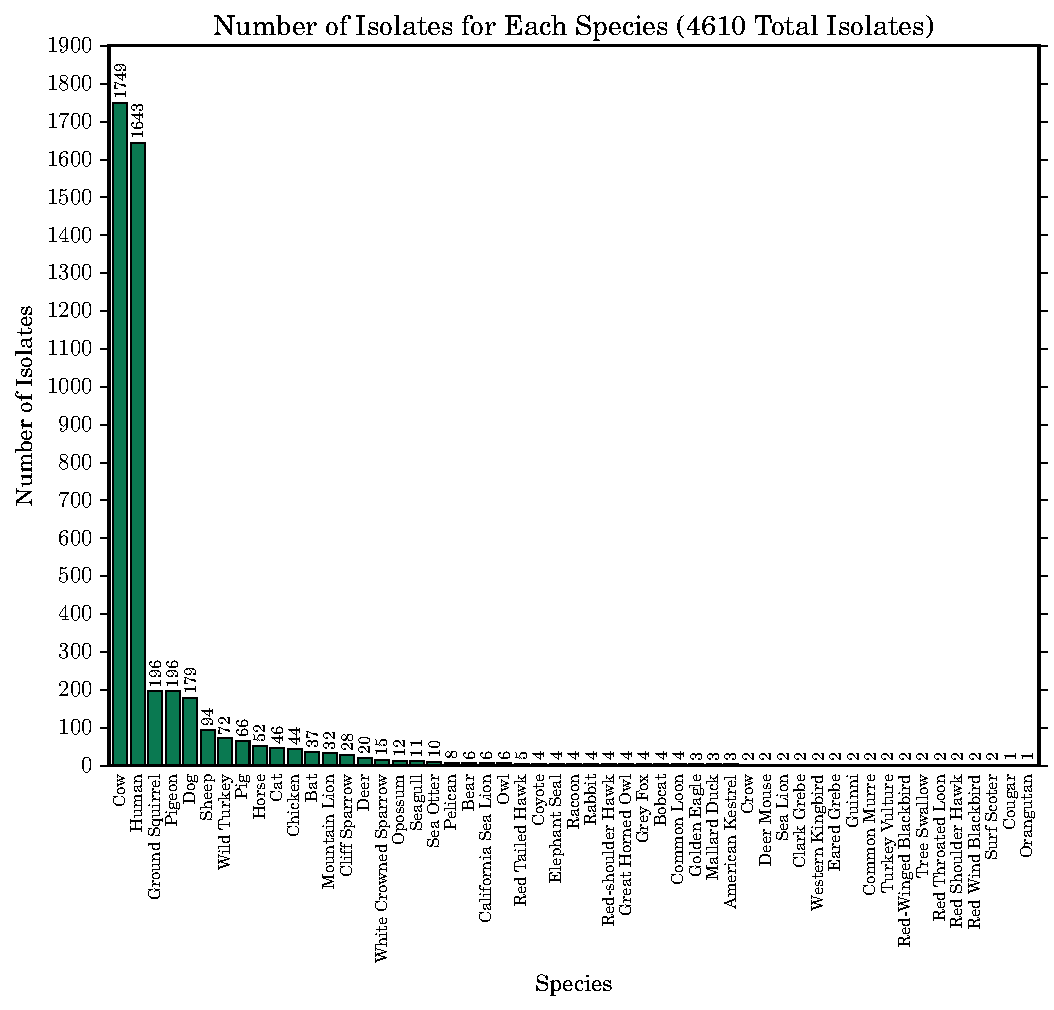
\includegraphics[width=\linewidth]{figures/bs/species_hist.pdf}
    \caption{
    A histogram of the number of \isols{} of each species in our study, taken from \cplop{}.
    There are 4,610 total \isols{} from 53 different \specs{}.}
    \label{fig:species}
\end{figure}

There are a total of 4,610 \isols{} in our dataset\footnote{A simplified version of \cplop{} containing \isol{} IDs, \spec{}, and \zscore{}s can be found at \texttt{https://github.com/jmcgover/cplop-acm-bcb-2016}.}. As seen from Figure \ref{fig:species},
the organic growth of \cplop{} yielded disproportionately many \ecoli{} isolates originating
from humans and cows (however, as shall be seen below, these isolates belong to a large number of strains). Each \isol{} is represented in \cplop{} with two \pyros{} ---  one each for \its{1} and \its{2} 
region.

%%%%% CLUSTERING FOR BS %%%%%
\chapter{Clustering for \BSlongs{}}

%%%%% METHODOLOGY %%%%%
\section{Methodology}\label{sec:methodology:clustering}

In order to understand the make up of \bslongs{} in \cplop{}, we chose to investigate how a density-based clustering algorithm might group the \isols{} we have collected so far and how that might affect a rudimentary \mst{} technique based off of clustering: cluster an unknown \isol{} along with the \isols{} in \cplop{} and classify it as the most plural species of the cluster.
Density-based clustering ties in well with our notion of closely-related strains of \ecoli{} (the relation being the separate \pearson{} comparison of each \itsshort{} region we use to compare \isols{}).
\index{\ecoli{} strain}
From the computer science point of view, a bacterial strain is essentially a cluster of \ecoli{} \isol{} representations stored in \cplop{}.
Our \mst{} method, thus, works as follows:
\begin{enumerate}
    \item \textbf{Strain Identification.} Identify bacterial strains in \cplop{} by clustering
    all \cplop{} \isols{}.
    \item \textbf{MST.} Given an isolate of unknown origin, find the cluster it belongs to.
    Return the \spec{} of the plurality of isolates in the cluster.
\end{enumerate}

Our clustering algorithm is the density-based clustering algorithm developed by Johnson \cite{johnson2015density}.
It extends \dbscan{} for the case of two \compfuncs{} between data points (our isolates are compared based on the two \itsshort{} regions) and implements an efficient spatial data structure to manage the retrieval of the data points.

\dbscan{} can easily use an efficient range query technique to find nearby points and speed up clustering time considerably by taking advantage of the \trieq{} that proper metric spaces have.
Unfortunately, \pearson{} does not encode a metric space, because it fails the \trieq{}\footnote{$d(x,z)\leq d(x,y) + d(y,z)$}. 
This complicates range queries, discussed in \autoref{sec:background:dbscan}, because spatial indexes tend to rely on the \trieq{}, usually with \euclid{}, to argue that certain points can be ignored during a spatial index tree traversal. 

To allow us the use of a spatial data structure with the \pearson{} to store data points during the clustering procedure we use instead the \clustplop{}, which we derive by recognizing in \autoref{eq:pearson} that \pearson{} is made up of \zscores{} of \pcveca{} and \pcvecb{}. 
The \zscore{} of \pcveca{} is:
\[
\zscoreeq{\pca}
\]
where \vecavg{\pca} and \vecstddev{\pca} are the mean and standard deviation of the values in a single pyroprint respectively. 
Thus, for clustering, we compare \pyros{} using the Euclidean distance \euczfunclabel{} of $z$-scores.
\begin{equation}\label{eq:euclidean_zscores}
\eucz{\pca}{\pcb}
\end{equation}
where \numdims{} is the number of dimensions.
This allows us to use spatial indexes and \bigo{\log{n}} lookup in \dbscan{}.

Each \isol{} is represented in \cplop{} by a pair of \pyros{}: one each from each \Ssixt{} and \Sfive{} region, complicating the use of \dbscan{} and the meaning of $\alpha$ threshold.
We handle this in \dbscan{} by performing two range queries, one each for \Ssixt{} and \Sfive{}, taking the intersection of the two results.
We must, however, pick a suitable \eps{} for each \itsshort{} region.

\cplop{} uses a threshold value of $\alpha = 0.995$  to compare two \pyros{}.
\Pyros{} with \pearson{} above $\alpha$ are considered to represent the same \dna{} material, while \pyros{} with a \pearson{} below $\alpha$ are considered to represent different \dna{} material \cite{Shealy:SeniorProject, soliman2013cplop, SolimanDVMBNWKG12}.

The number of dispensations \numdims{} used to build a \pyro{} differ for the \Ssixt{} and \Sfive{} regions.
Because  $\numdims{}_{\Ssixt{}} \neq \numdims{}_{\Sfive{}}$, the original $\alpha$ under the space defined by \eqref{eq:euclidean_zscores} no longer applies in the same way to both regions.
An alternative formulation of \eqref{eq:euclidean_zscores}, with respect to the \pearson{} \pcfunclabel{}, is:
\begin{equation}\label{eq:euclidean_zscores_alternate}
\euczalternate{\pca}{\pcb}
\end{equation}
where \numdims{} is the number of dimensions and $\numdims{}_{\pcveca{}} = \numdims{}_{\pcvecb{}} = \numdims{}$. 
Using \autoref{eq:euclidean_zscores_alternate}, we can convert $\alpha$ to the values in \autoref{tab:converted_thresholds}. 
We use these converted $\alpha$ values as the \eps{} for each \itsshort{} region's \codefn{RangeQuery}.
\begin{table}
\centering
\caption{Converted $\alpha$ threshold to fit the new metric space defined by \eqref{eq:euclidean_zscores}.}
\label{tab:converted_thresholds}
\begin{tabular}{|c|c|c|}
\hline
\textbf{\itsshort{} Region} & \Ssixt{}     & \Sfive{}     \\
                            & $\alpha$     & $\alpha$     \\ \hline
\pcfunc{\pca}{\pcb}         & 0.995        & 0.995        \\ \hline
\numdims{}                  & \Ssixtdims{} & \Sfivedims{} \\ \hline
\euczfunc{\pca{}}{\pcb{}}   & 0.9747       & 0.9644       \\ \hline
\end{tabular}
\end{table}

When clustering \cplop{} isolates using our density-based clustering algorithm, we need to set up the two parameters at our disposal: \minneigh{} and \eps{}.
For \eps{} we choose the two values shown in Table \ref{tab:converted_thresholds} converted from the 0.995 \pearson{} threshold of pyroprint similarity. 
Essentially, we only want to consider the \eps{}-neighborhood of a \pyro{} that contains the other \pyros{} that we consider to represent the same DNA material.

For the \minneigh{} parameter, we use \textit{grid search} running our clustering with \minneigh{} set to $1, 2, 3, 4, 5, 6$, and $7$.
The \minneigh{} value adjusts how strict our definition of a cluster is.
That is, the higher the value of \minneigh{}, the more neighbors a core point must have with \eps{} of it and its neighbors to become a cluster.
Balancing this value with the coverage of our algorithm is crucial to its success, because for too low of a value, we may not have a clear plurality in a cluster, while too high of a value may miss some smaller clusters that might classify our unknown \isol{} into something other than noise.


%%%%% EVALUATION %%%%%
\section{Evaluation}\label{sec:evaluation:clustering}
Clustering for \bslongs{} has two aspects that we must evaluate: how pure the \bslongs{} (clusters) are and how many of the \isols{} in \cplop{} end up in a cluster (as opposed to noise).
The former tests whether the \ecoli{} strains stay relatively unique to the \spec{} from which they come from, the core theory of library-based \mst{}.
The latter tells us how effective 
\autoref{sec:methodology:clustering} describes how we can use clustering as a \mst{} method --- cluster an unknown \isol{} along with the \isols{} in \cplop{} and classify it as the most plural species of the cluster.
Cluster purity can easily gauge how effective this technique is at \mst{}, since the concept readily summarizes to how pure, from a \spec{} perspective, a cluster is.
\Dbased{} clustering algorithms such as \dbscan{} may not cluster every datapoint, as mentioned in \autoref{sec:background:dbscan},  labeling some datapoints (\isols{}) as noise and thus leaving them unclustered.
%Thus, it is crucial that our \mst{} method has the ability to assert a classification on any \isol{} we provide it, driving us to use \kNN{} for classification.
%Nevertheless, by applying \dbscan{} to \cplop{} \isols{}, we gained insight into the nature of \ecoli{} strains that we discuss in \autoref{sec:results:clustering}.

\subsection{Cluster and Clustering Purity}
In this paper we look at the results of clustering \cplop{} data using this algorithm from the perspective of cluster purity. We call a cluster (\bslong{}) \textit{100\% pure}
if all isolates that belong to it come from the same \spec{}. 

Of interest to us is the following information:
\begin{enumerate}
    \item The number of 100\% pure clusters and the percentage of bacterial isolates from \cplop{} clustered into pure clusters.
    \item The structure of impure clusters: specifically, whether a dominant \spec{} can
    be clearly identified in each cluster.
    \item Coverage: the total number of \cplop{} isolates found to belong to a strain.
    \item MST Accuracy: the percentage of isolates for which the strain-based MST procedure produces the correct response.
\end{enumerate}
Thus, our core measure is \textit{cluster purity}, the proportion of a cluster that comes from the most plural \spec{} of that particular cluster.
\index{cluster purity}
A \textit{100\% pure cluster} is a cluster which only contains data points (\isols{}) with the same class label (same \spec{} of origin). 

Consider a cluster $C=\{c_1,\ldots, c_K\}$. Let $s(c)$ refer to the species of isolate $c$.
Let $m$ be the plurality species label for data points in $C$, and let the total number of points in
$C$ with $s(c) = m$ be $s_m$. Then the \textit{individual cluster purity} $\nu$ of cluster $C$ is:
\[
    \nu(C) = \frac{s_m}{K}
\]

In addition to computing the purity of individual clusters we want to have an understanding of the overall purity on the entire dataset.
Given a \textit{clustering} $\mathcal{C} = \{C_1,\dots,C_n\}$ on a dataset, we define the size $\mathcal{M}$ of the set of clusters: 
\index{clustering}
\begin{equation}\label{eq:num_isols}
\mathcal{M} = \sum_{i = 1}^{n} |C_i|
\end{equation}
The \textit{overall clustering purity} is:
\index{overall clustering purity}
\begin{equation}\label{eq:overall_clustering}
\sum_{i=1}^{n} \frac{|C_i|}{\mathcal{M}}\cdot\nu(C_i)
\end{equation}
One can think of \eqref{eq:overall_clustering} as a form of weighted arithmetic mean of the purities, where the size of the cluster adds more weight to the value.

\subsection{Clustering Coverage}

% COVERAGE --------------------
%\subsection{Clustering Coverage} 
\label{sec:validation:coverage}
Coverage of the dataset is important to an effective \mst{} method.
The density-based clustering method we use has one key disadvantage: a clustering run  with the parameter \minneigh{}, treats all points that do not fit into a cluster of size  of at least \minneigh{} as noise.
This means that as the value of \minneigh{} grows, so will the number of \isols{} that do not cluster into a strain.

Given the parameter \minneigh{} of the clustering algorithm, we collect the following four measures, that collectively represent the breakdown of all data points (\isols{}) in \cplop{}:
\begin{enumerate}
    \item \textit{Noise.} Number/percentage of \isols{} clustered as noise points.
    \item \textit{Misses.} Number/percentage of \isols{} from  minority species
    in impure clusters.
     \item \textit{Hits.} Number/percentage of \isols{} from plurality species in
     impure clusters.
     \item \textit{Pure points.} Number/percentage of \isols{} in 100\% pure clusters.
\end{enumerate}
\index{noise}
\index{misses}
\index{hits}
\index{pure points}


%%%%% RESULTS %%%%%
\section{Results}\label{sec:results:clustering}
In gauging how effective our clustering method is against \cplop{}, we looked at the distribution of cluster sizes, the number of \isols{} that fell into high purity clusters, the number of unique species in each cluster and how that affected the size and purity, and overall coverage and accuracy metrics.
From these data, we gained some insight into the clustering algorithm and were able to visualize some predictions we had about the biological aspects of strains.  

% SIZES --------------------
\subsection{Cluster Size Distribution}
\begin{sidewaysfigure}
    \centering
    \subfloat[
        Cluster Size Distribution for \minneigh{} of 3
        ]{
        \label{fig:clust_size_dist_3}
        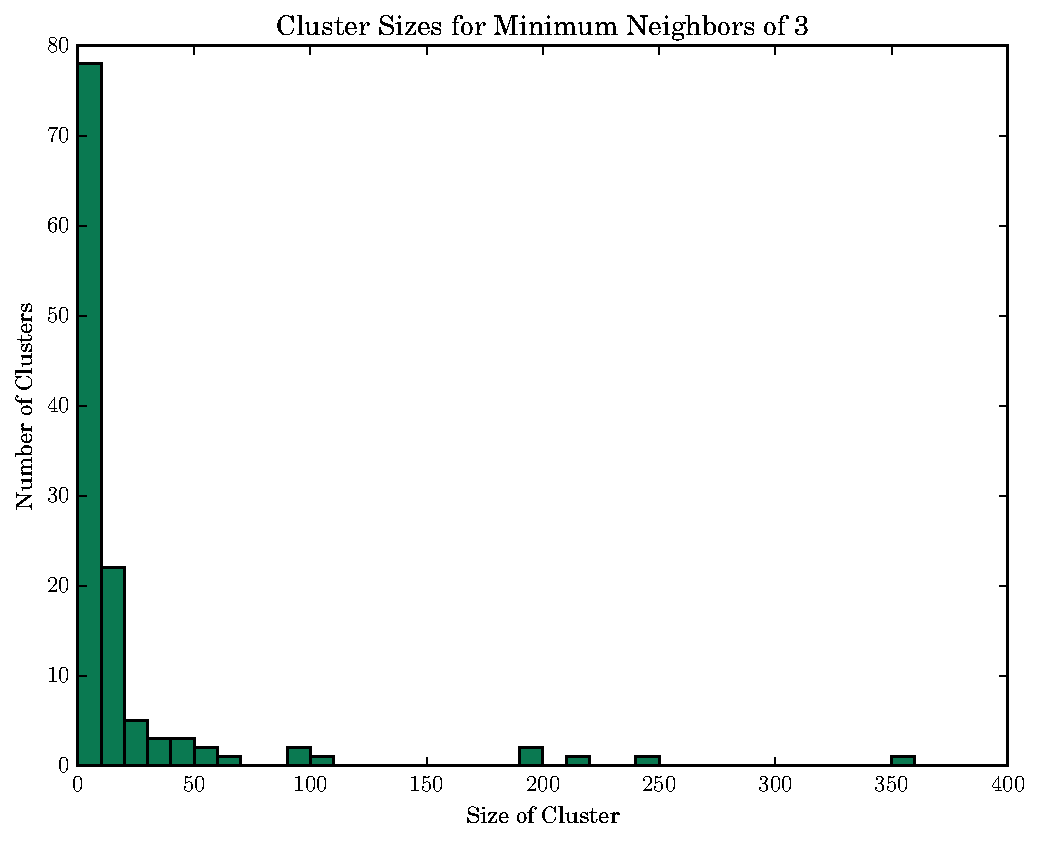
\includegraphics[width=0.30\linewidth]{figures/bs/neigh_size_3}
        }
    \hfill
    \subfloat[
        Cluster Size Distribution for \minneigh{} of 5
        ]{
        \label{fig:clust_size_dist_5}
        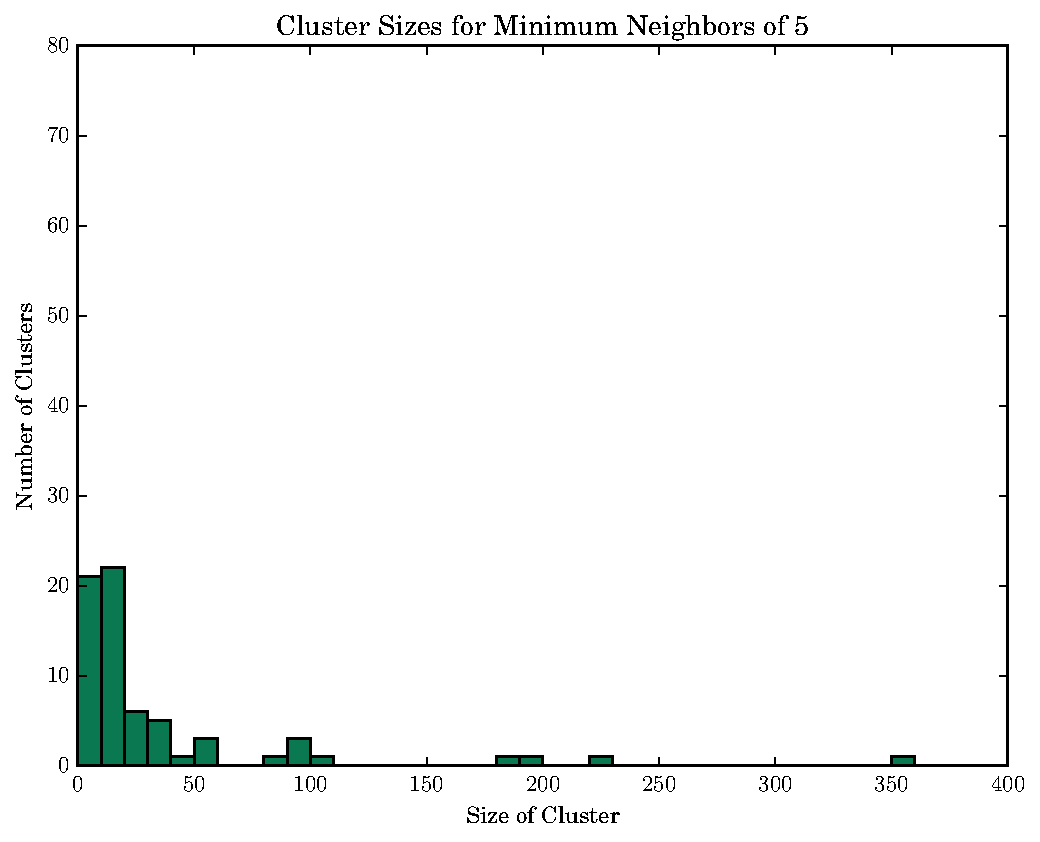
\includegraphics[width=0.30\linewidth]{figures/bs/neigh_size_5}
    }
    \hfill
    \subfloat[
        Cluster Size Distribution for \minneigh{} of 7
        ]{
        \label{fig:clust_size_dist_7}
        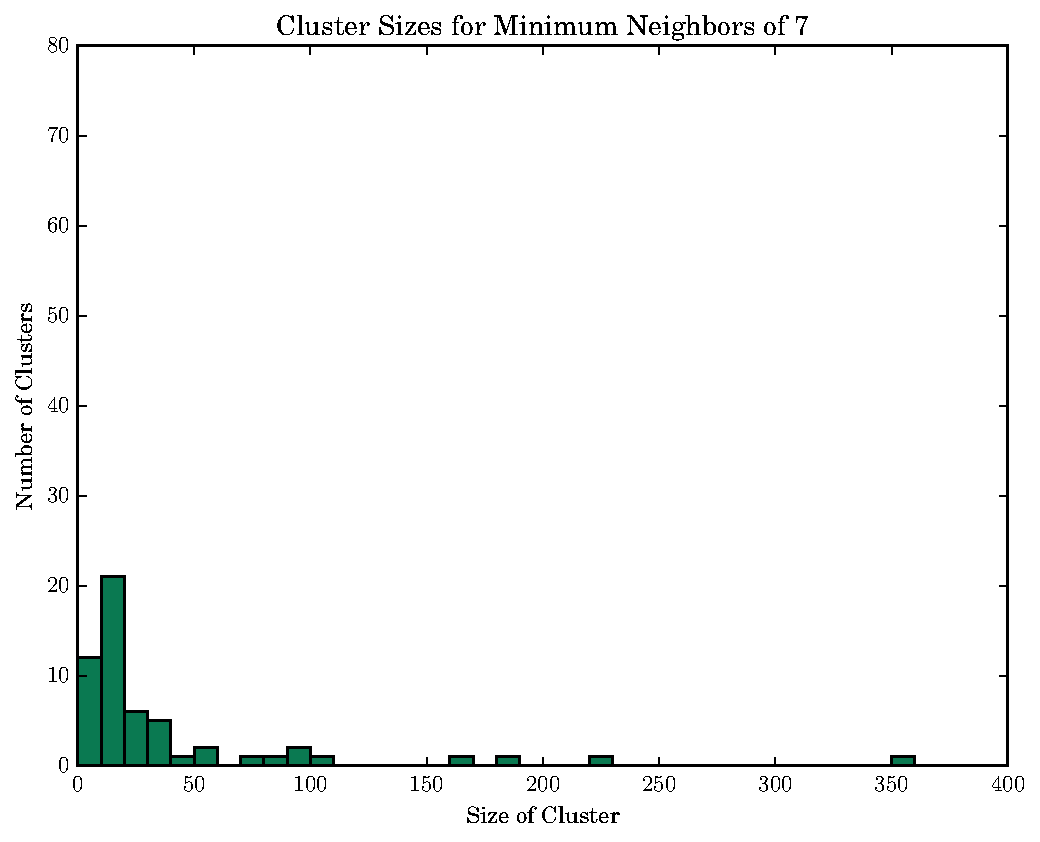
\includegraphics[width=0.30\linewidth]{figures/bs/neigh_size_7}
    }
    \caption{The size distribution of clusters skews heavily towards smaller clusters.}
    \label{fig:clust_size_dist}
\end{sidewaysfigure}

\autoref{fig:clust_size_dist} shows the distribution of cluster sizes as \minneigh{} increase from 3, to 5, to 7. 
We see that at all three \minneigh{} values, the number of small clusters (fewer than 10) dominates the overall makeup of clusters.
\autoref{fig:clust_size_dist} shows a propensity towards small clusters at low \minneigh{} values.
This creates a high number of 100\% or almost 100\% pure clusters.
Most clusters are tiny, with a few larger clusters for small \minneigh{} values.

As we approach higher \minneigh{} values, the smaller clusters disappear.
As \minneigh{} increases from 3 to 5, we lose over half of clusters of size smaller than 10; while as \minneigh{} increases to 7, we lose only a few more.
Furthermore, while the number of clusters with 10-20 \isols{} stays relatively stable across \minneigh{} values, the number of clusters with 50-100 \isols{} increase for \minneigh{} of 5 and 7.

% PURITIES --------------------
\subsection{Cluster Purity Distribution}
\begin{sidewaysfigure}
    \centering
    \subfloat[
        Cluster Purity Distribution for \minneigh{} of 3
        ]{
        \label{fig:clust_purity_dist_3}
        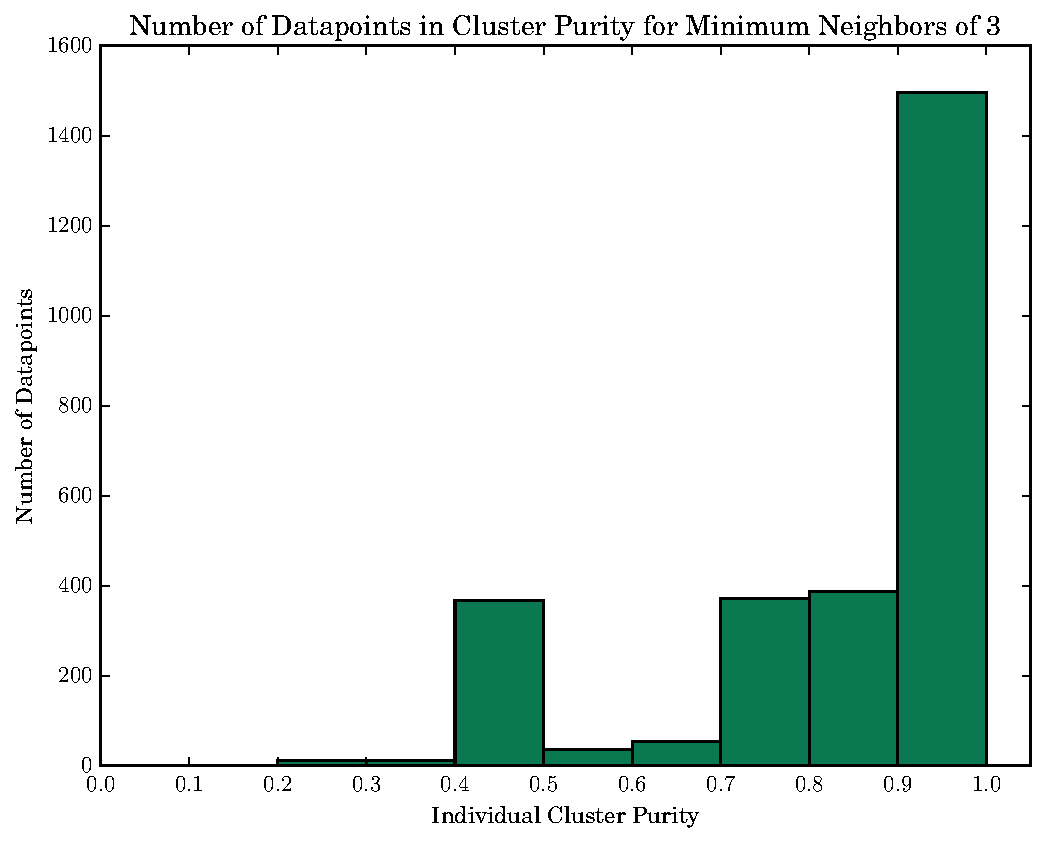
\includegraphics[width=0.30\linewidth]{figures/bs/neigh_dist_data_3}
    }
    \hfill
    \subfloat[
        Cluster Purity Distribution for \minneigh{} of 5
        ]{
        \label{fig:clust_purity_dist_5}
        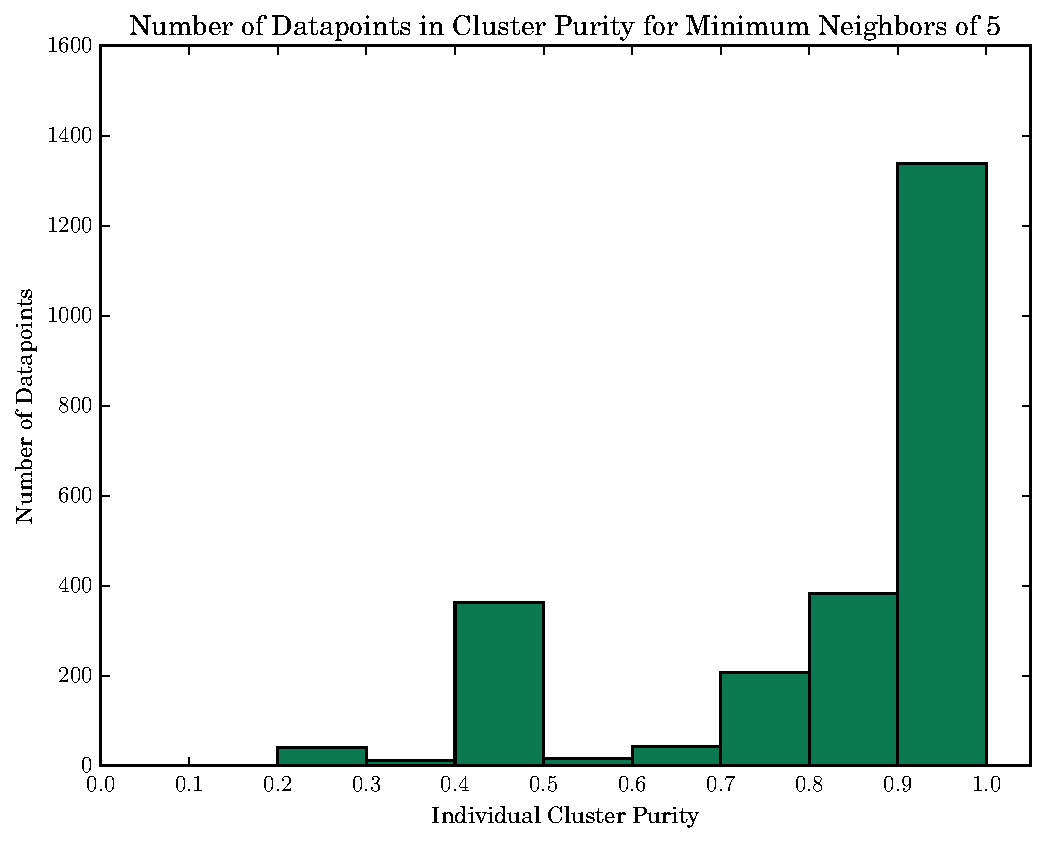
\includegraphics[width=0.30\linewidth]{figures/bs/neigh_dist_data_5}
    }
    \hfill
    \subfloat[
        Cluster Purity Distribution for \minneigh{} of 7
        ]{
        \label{fig:clust_purity_dist_7}
        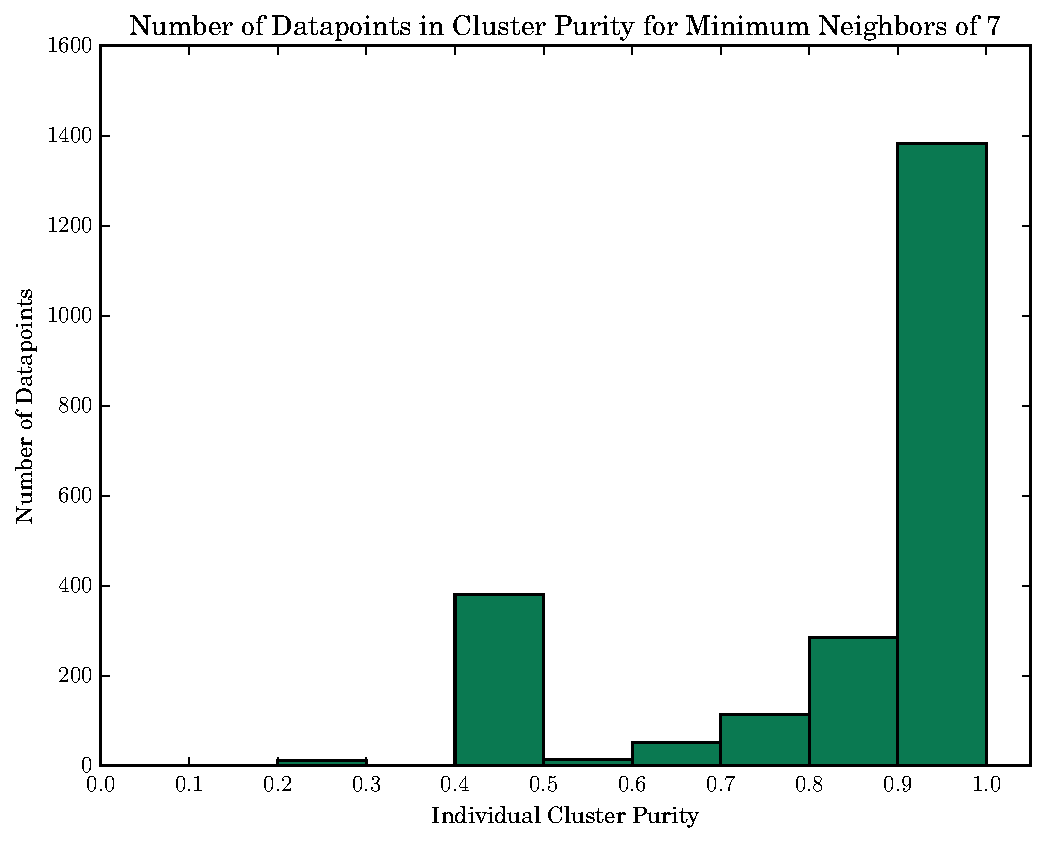
\includegraphics[width=0.30\linewidth]{figures/bs/neigh_dist_data_7}
    }
    
    \caption{The number of \isols{} that fall into a cluster of a given purity. We notice that that the number of \isols{} that fall into the 0.90 to 1.00 cluster purity range decreases as we increase \minneigh{} from 3 to 5, but increases from 5 to 7.}
    \label{fig:clust_purity_dist}
\end{sidewaysfigure}

Of interest to our investigation is the number of \isols{} that fall within clusters of a particular purity. 
\autoref{fig:clust_purity_dist} shows the number of \isols{} that fall within a cluster of a particular purity as a histogram.
We notice that as \minneigh{} increases, the purity skews towards purer clusters and that a portion of \isols{} remain in an impure cluster regardless of the \minneigh{} value.

From \minneigh{} of 3 all the way to 7, there are about 400 \isols{} that land in a cluster of purity between 0.4 and 0.5.  
This group of isolates remains largely unchanged as we restrict the \minneigh{} value.
We suspect (and discuss in \autoref{sec:discussion:clustering}) that certain \ecoli{} strains find themselves in many \spec{} fecal matter.

% UNIQUE --------------------
\subsection{Unique Species in Each Cluster}\label{sec:results:unique}

\begin{sidewaysfigure}
    \centering
    \subfloat[
        Cluster Purity for \minneigh{} of 3
        ]{
        \label{fig:clust_pure_3}
        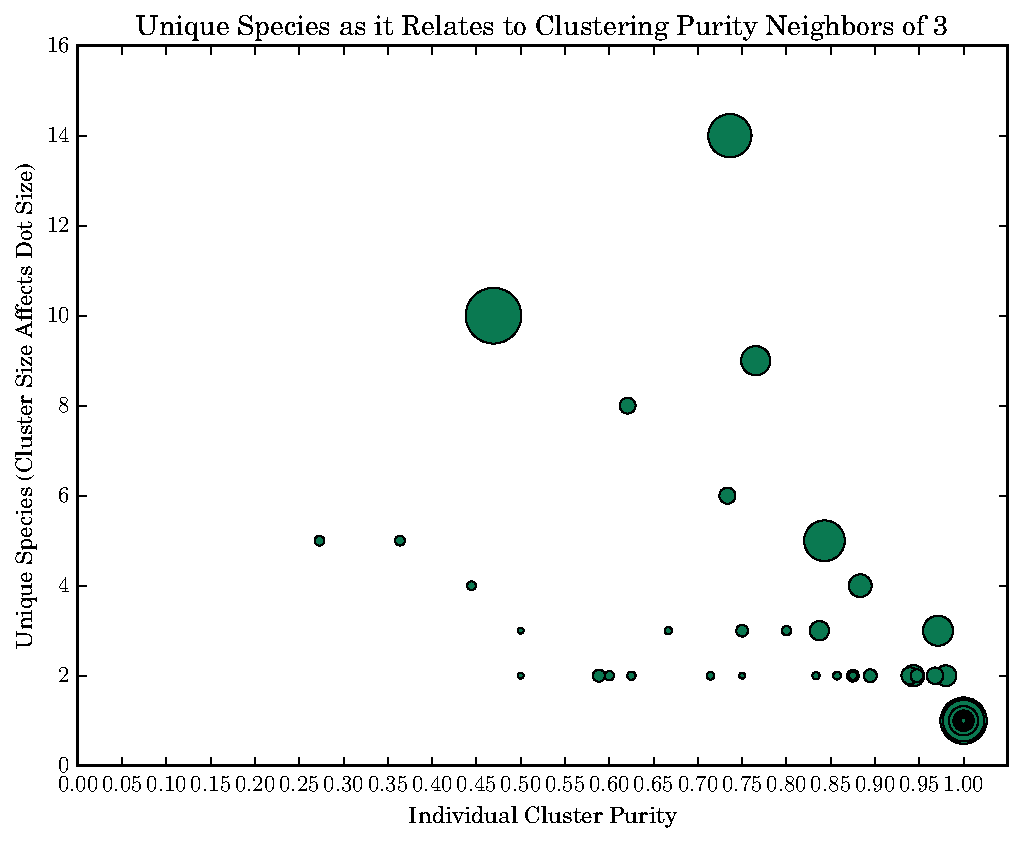
\includegraphics[width=0.30\linewidth]{figures/bs/neigh_purity_unique_3_size}
    }
    \hfill
    \subfloat[
        Cluster Purity for \minneigh{} of 5
        ]{
        \label{fig:clust_pure_5}
        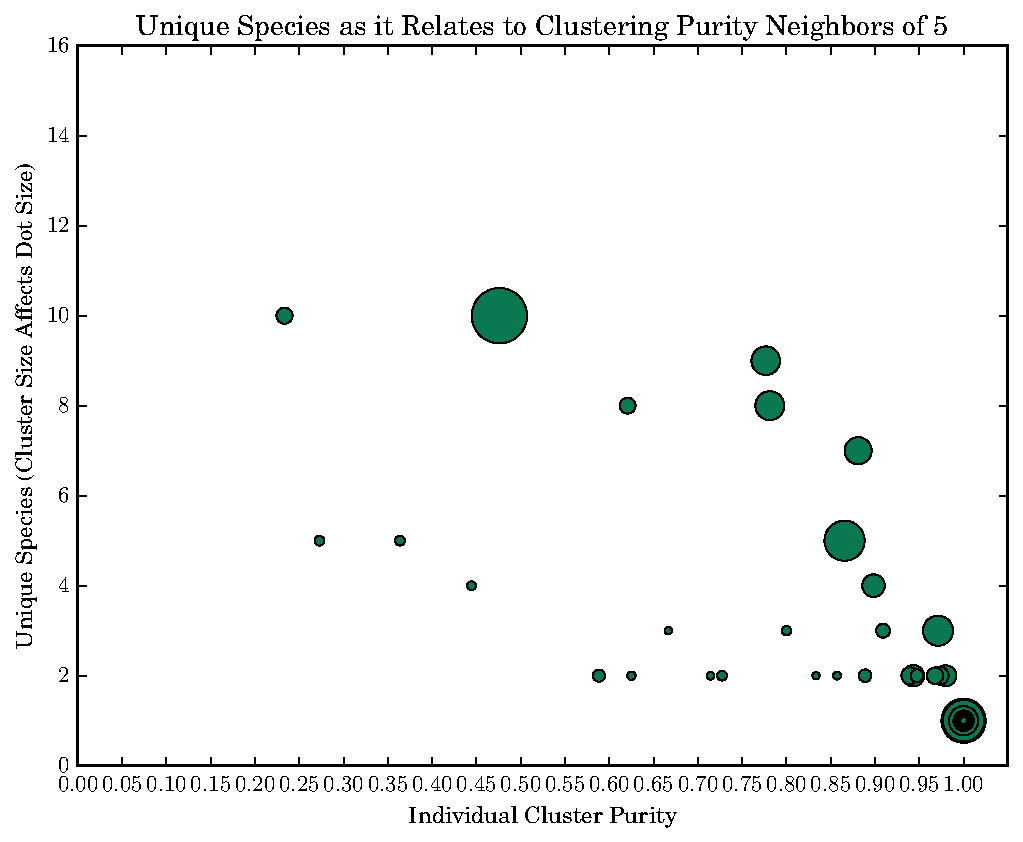
\includegraphics[width=0.30\linewidth]{figures/bs/neigh_purity_unique_5_size}
    }
    \hfill
    \subfloat[
        Cluster Purity for \minneigh{} of 7
        ]{
        \label{fig:clust_pure_7}
        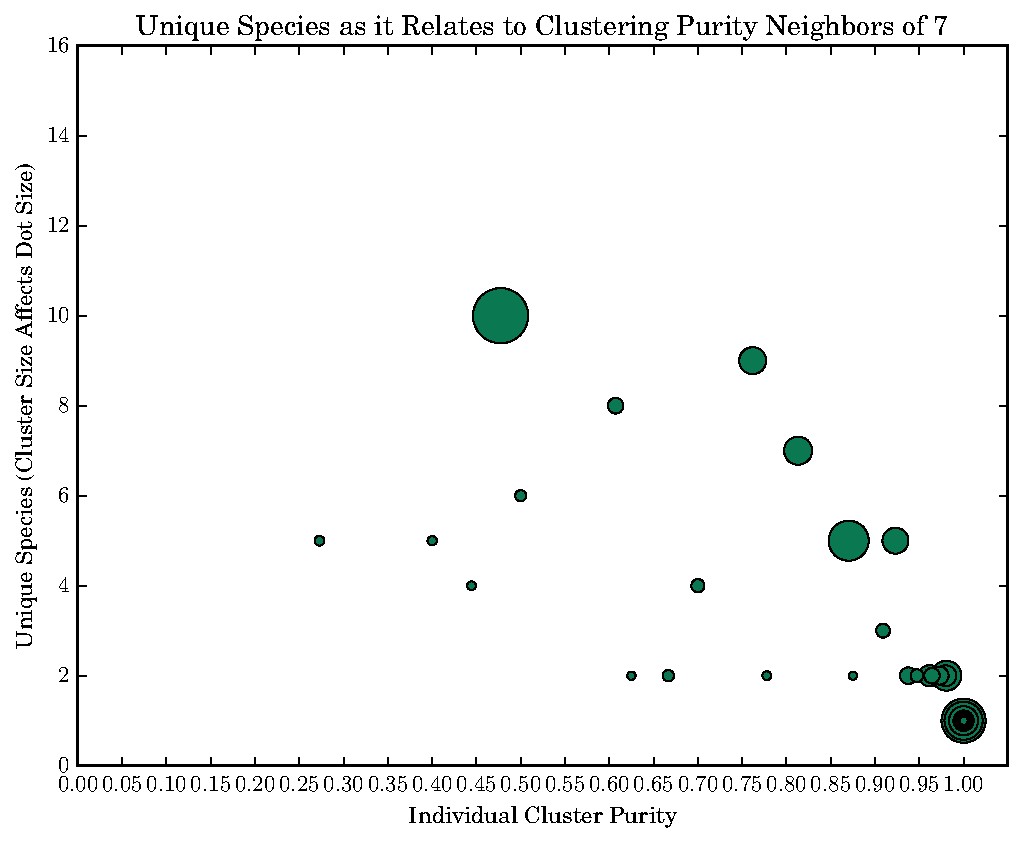
\includegraphics[width=0.30\linewidth]{figures/bs/neigh_purity_unique_7_size}
    }

    \caption{These three dimensional graphs show the individual cluster purity in the horizontal axis, the number of unique species in the vertical axis, and the relative size of the cluster in the diameter of the dots. Each individual dot is its own cluster. We find that as we restrict cluster to needing more neighbors (increasing the \minneigh{} value), we lose some clusters and gain more pure clusters.}
    \label{fig:clust_pure}
\end{sidewaysfigure}

Knowing the number of unique \spec{} in our clusters is key to understanding how our
strain-based \mst{} algorithm  performs.
\autoref{fig:clust_pure} plots the number of unique species in each cluster (vertical axis) against
individual cluster purity (horizontal axis) representing each cluster as a circle of diameter
proportional to cluster size\footnote{A linear scaling of the diameter with respect to \textit{the largest cluster amongst all the clusterings} defines the diameters of the dots.}.
The points at the lower right represent many clusters of various size of 100\% (or near so) purity and are stacked from largest behind cluster to smallest in front.

As \minneigh{} values increase  we see one cluster at the top right
(\minneigh{}=3) with 14 unique species disappear  as \minneigh{} becomes $5$.
One very low purity cluster at a \minneigh{} value of 5 disappears 
when we increase \minneigh{} to 7 in \autoref{fig:clust_pure_7}.

A particularly large cluster at around 0.45 purity with 11 unique \spec{}, remains relatively intact
(and is clearly recognizable)
as \minneigh{} changes from 3, to 5, to 7. 
This can account for the large amount of \isols{} clustered into impure clusters in \autoref{fig:clust_purity_dist}.

As we restrict the cluster size with \minneigh{}, we see that this appears to break up some clusters and cause others to become bigger.
It is difficult to track exactly how a cluster changes without making some simplifying assumptions or without tracking all 4,610 \isols{} as they move from cluster to cluster.

% COVERAGE --------------------
\subsection{Clustering Coverage}
\begin{figure}[ht!]
    \centering
    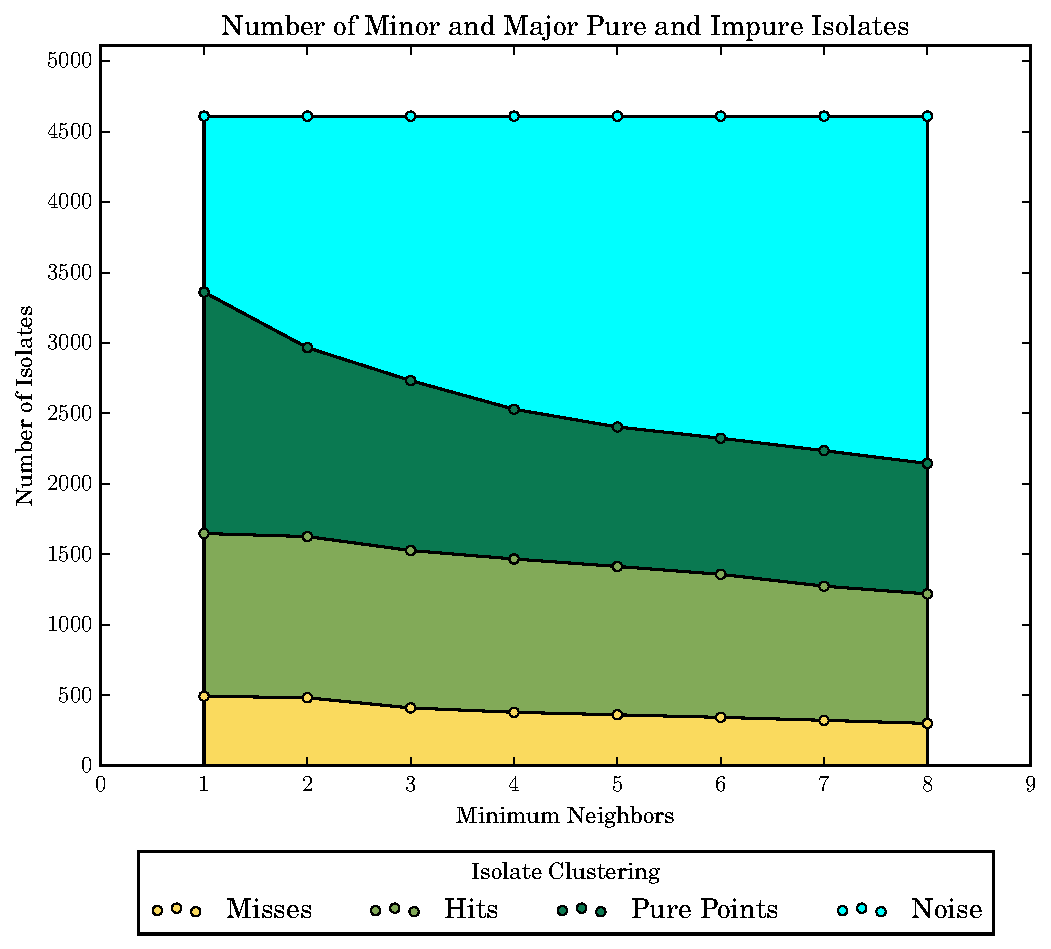
\includegraphics[width=\linewidth]{figures/bs/neigh_minor_major_impure_filled_stack}
    \caption{As \minneigh{} increases, we see that we cluster fewer \isols{}. throughout, the number of major pure \isols{} stays relatively equal to the number of major impure \isols{}.}
    \label{fig:clustered}
\end{figure}

Clustering coverage is important to consider, since we want our clustering algorithm to apply to as many \isols{} as possible.
Towards this end we investigated the four metrics introduced in \autoref{sec:validation:coverage} --- noise, misses, hits, and pure points --- for each \minneigh{} clustering investigated.
We hope to find the \minneigh{} value that gives us the most pure points, but will also settle for the fewest misses, shown in \autoref{fig:clustered}.

The cyan area is noise --- \isols{} that were not clustered. 
The dark green area is the proportion of pure points. 
Light green is the number of hits.
Gold is the number of misses.

\autoref{tab:coverage:values} displays the number of \isols{} that fall into the categories in \autoref{fig:clustered}.
\input{tables/coverage-values}
\autoref{tab:coverage:percent:total} shows the percentage of \textit{all} \isols{} that ended up in a cluster where their \spec{} was the minority, the most dominant, and that make up the entirety of the cluster and those categorized as noise.
\input{tables/coverage-percent-total}
\autoref{tab:coverage:percent:total} shows the percentage of \textit{clustered} \isols{} that ended up in a cluster where their \spec{} was the minority, the most dominant, and that make up the entirety of the cluster.
\input{tables/coverage-percent-clustered}
\autoref{tab:coverage:percent:clustered:noise} compares the percent of all \isols{} that \dbscan{} placed in a cluster and determined to be noise, while \autoref{tab:coverage:values:clustered:noise} shows the actual values.
\input{tables/coverage-percent-clustered-noise}
\input{tables/coverage-values-clustered-noise}

It is good to note that the number of misses are low and flatten out as we increase \minneigh{} from a value of 3, giving us good reason not to investigate clustering where \minneigh{} is greater than we have already investigated.
The number of pure points stays relatively equal to the number of hits.
Important in \autoref{fig:clustered} is the amount of \isols{} that the algorithm does cluster.
The combination of the gold and two green areas show the total number clustered, while the cyan shows the number of \isols{} that were \textit{not} clustered.
It is unfortunate that the number of noise \isols{} is high, but we plan to mitigate that in future work.

% OVERALL --------------------
\subsection{Overall Clustering Purity}
\begin{figure}[ht!]
    \centering
    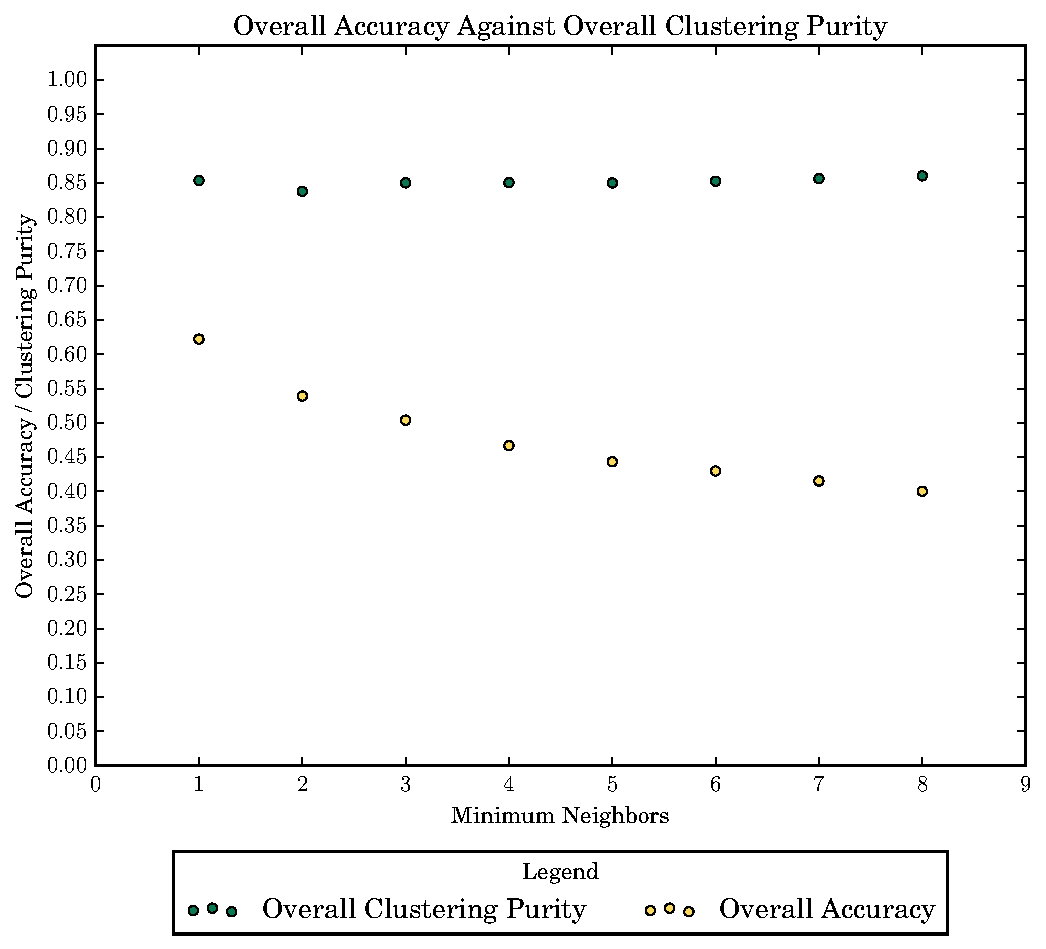
\includegraphics[width=\linewidth]{figures/bs/neigh_clust_accuracy.pdf}
    \caption{The overall accuracy decreases as we restrict  \minneigh{}. 
    The overall clustering purity stays relatively the same as we increase the value for \minneigh{}. 
    That is, for clustered \isols{}, the classification algorithm stays relatively the same relative to the number of isolates accurately clustered.}
    \label{fig:overall}
\end{figure}

Overall clustering purity, defined in \autoref{eq:overall_clustering}, is the number of \isols{} clustered that end up in a cluster where their \spec{} is the most plural \spec{}. 
The overall accuracy is the proportion of correctly classified \isols{} out of all the \isols{} under consideration.
We want to maximize both values, but would prefer the former over the latter.
Coverage is an issue we are concerned about, but we plan to mitigate this issue by leveraging  \cite{DBLP:conf/bibm/McGovernDKBVG15} against clusters of \isols{}.
%Using \cite{DBLP:conf/bibm/McGovernDKBVG15}, we can simplify the number of comparisons needed by comparing to clusters of \isols{} instead of \isols{} themselves.

\autoref{fig:overall} shows the overall accuracy compared to the overall clustering purity. 
A \minneigh{} value equal to 3 is the last \minneigh{} value where the overall accuracy stays above 0.50.
It is not for a lack of correctness, as \autoref{fig:clustered} shows, but more that \isols{} simply are not being clustered as we restrict the \minneigh{} value.
In fact, the overall clustering purity in \autoref{fig:overall} stays relatively constant.
This means that if an \isol{} is clustered by our algorithm, it will likely be clustered with other \isols{} of the same \spec{}.



%%%%% DISCUSSION %%%%%
% STRAINS --------------------
\section{Discussion}\label{sec:discussion:clustering}

In general, we observe two trends in our data. For the \isols{} that get clustered into strains,
our approach correctly identifies the \spec{} with over 80-85\% accuracy. This accuracy
is sufficient to conduct sophisticated \mst{} studies. Most of the strains discovered 
in the \cplop{} data show high degree of purity, and even considering the presence of 
a few large impure clusters, most of the clustered \isols{} fall into strains of high purity.


At the same time, the pure strain-based approach suffers from a drop in the coverage as the size of a cluster grows. 
This means that in general \cplop{} \isols{} tend to be very diverse
and come from strains for which not enough DNA material has been collected and pyrosequenced.
Identifying the \spec{} for \isols{} that do not fall into strains/clusters using the pure strain-based
method is impossible. In future work, our goal is to combine the \kNN{}-based \mst{} method
of \cite{DBLP:conf/bibm/McGovernDKBVG15} with the strain-based approach discussed in this paper
to increase coverage while preserving the high \mst{} accuracy.




%%%%%%%


%Considering how many \isols{} end up in clusters of high purity, as \autoref{fig:clust_purity_dist_3} shows, this occurrence appears to be infrequent.
%Nevertheless, viewing the progression of graphs in \autoref{fig:clust_pure} implies that the clusters morph and change into each other as we increase \minneigh{}.

One factor explaining the large impure clusters is the possibility that these
clusters represent what the  biologists call  ``transient'' strains, i.e., strains that 
persist in more than one \spec{}. 
%That is, certain strains might show up in many \spec{} and not just relegated to one \spec{}.
Such a characteristic can compound \mst{} by making certain strains of \ecoli{} less reliable as \fib{} for identifying \spec{}.
In \autoref{fig:clust_purity_dist}, we see evidence of that and it is revealed in \autoref{fig:clust_pure}.
One mitigation strategy may be to reduce the presence of these strains in library holding the \fib{}.
Another may be to fall back to an alternative \mst{} technique that works with \cplop{} when an unknown \isol{} falls into an impure cluster.  Finally, if a true transient strain is indeed
discovered, and an \isol{} is mapped to it, our \mst{} procedure can simply acknowledge the
that the query \isol{} belongs to a transient strain and provide information about the \spec{}
that show high frequency of \ecoli{} incidence from this strain.



%It also is possible that a more complicated or biologically-motivated strategy may work best.
%One avenue of validation we chose not to pursue was $k$-fold cross-validation.
%Previous work \cite{DBLP:conf/bibm/McGovernDKBVG15} has used it for validation.
%Future work may include it, but large $k$ values are likely to partition the dataset into groups different enough to create widely varying clusterings.
%%%%% KRRRAAAAAPPPPPP %%%%%
\chapter{The \kraplong{}}\label{chap:krap}

%%%%% METHODOLOGY %%%%%
\section{Methodology}\label{sec:methodology:krap}
Due to the two-\itsshort{}-region nature of \ecoli{} \isols{} in \cplop{}\footnote{see \autoref{sec:isolates}}, we effectively have two \compfuncs{} between datapoints (\isols{}), complicating our use of \kNN{}.
\kNN{} provides \cplop{} biologists a transparent and intuitive way of understanding the \spec{} classification it asserts, so we find that it will be a usefully insightful .
Applying \kNN{} to \cplop{} \isols{} gives us two lists, one for each \itsshort{} region, that we must make a classification from.
In order to accommodate multiple \compfuncs{}, we need a multiple-\knnlong{} list resolution strategy.
Rather than create a new similarity metric out of a pair of similarity scores, which may deviate from the inherent nature of the \compfunc{}, we choose to update the \kNN{} method with four different ways of selecting the resultant category label: the \kraplong{} (\krap{}).
%We propose the \krap{}, four strategies to resolve these multiple \knnlong{} lists that multiple \compfuncs{} result in.
%Furthermore, \kNN{} provides \cplop{} biologists a transparent and intuitive way of understanding the \spec{} classification it asserts.
These four methods are described below.

In what follows, we generalize our problem. Given \UNKNOWN{} and \KNOWN{}, two library objects (\isols{}), and a collection of \compfuncs{}, \COMP{}$=(\COMP{}_1,\ldots \COMP{}_m)$, with $m > 1$, comparing \UNKNOWN{} to \KNOWN{} gives us a collection of values:  
$\COMP{}(\UNKNOWN{},\KNOWN{}) = (\COMP{}_1(\UNKNOWN{},\KNOWN{}),\ldots,\COMP{}_m(\UNKNOWN{},\KNOWN{}))$.
All four resolution procedures described in this section work with such a generalized representation of \isols{} and \compfuncs{} between them.

Given an unknown \isol{} \UNKNOWN{}, a library of classified\footnote{A ``classified \isol{}'' is an \isol{} for which the \spec{} has been identified in the database.} \isols{} \LIB{}, and a set of \compfuncs{} \COMP{}, we compare \UNKNOWN{} to each object in \LIB{} using each \compfunc{} in \COMP{}. To resolve these \compfuncs{}, we propose four algorithms:

\subsection{Comparing \Isols{}}
Comparing \isols{} to each other is of primary interest to biologists using \cplop{}.
%Of primary interest to the biologists using \cplop{} is comparing \isols{} to each other.
\cplop{} represents each \isol{} by a pair of mutually incomparable \pyros{}: one for each of the two \itsshort{} regions.
As a result, given \isols{} $I_1, I_2$, we can represent each as a pair of pyroprint vectors 
\[I_1 = (\vec{q}_1, \vec{q}_2) \text{ and } I_2 = (\vec{r}_1, \vec{r}_2),
\]
where $\vec{q}_1 \text{ and } \vec{r}_1$ are respectively $I_1 \text{ and } I_2$'s \Ssixt{} \pyro{} and $\vec{q}_2 \text{ and } \vec{r}_2$ are respectively $I_1 \text{ and } I_2$'s \Sfive{} \pyro{} \cite{Black2014121}. Since \pyro{}s from different regions are incomparable, comparing \isol{}s must be done as follows:
\[
\COMP{}(I_1, I_2) = (\pcfunclabel(\vec{q}_1, \vec{r}_1), \pcfunclabel(\vec{q}_2, \vec{r}_2)),
\]
where $\pcfunclabel(\cdot,\cdot)$ is between \pyros{} of the same \itsshort{} region and is the \pearson{}. Thus, when comparing \isol{}s, we effectively have two different similarity metrics, one for each \itsshort{} region:
\[
\COMP{}(I_1, I_2) = (\COMPsixt{}(I_1, I_2), \COMPfive{}(I_1, I_2)).
\]

\input{algorithms/comparison}

\subsection{\a{} Filtering}
Our first modification to \kNN{} is an additional condition at step \ref{knn:filter}, after finding the \knnlong{}:
\begin{enumerate}
\setcounter{enumi}{3}
\item Consider only the top $k$ entries in $N$ above threshold $\alpha$
\end{enumerate}
The $\alpha$ threshold allows biologists to filter out neighbors that are among the $k$ closest, but too dissimilar to compare. 
When comparing multiple \pyro{}s of the same region of a single \isol{} for quality control, the \pearson{} between them is strictly above 0.995.
As a result, for many other studies --- not necessarily MST-focused --- \cplop{} researchers use a \pearson{} of 0.990 or above to define a strain of \ecoli{}.
Filtering by some value near this may give more accurate results and provides an intuitive way to relate these lists to other studies.
\input{algorithms/filter}

\subsection{\rmean{}}
For \UNKNOWN{} and a $\SOMEPYRO\in\LIB{}$, we take the mean of the result of all of the \compfuncs{} and build a single \knnlong{} list from it.
The mean can be any metric mapping $\R^n\times\R^n\rightarrow\R$ and in the investigated implementation, we use the euclidean distance, also known as the $L^2$ norm.
A single \knnlong{} list results from this algorithm that we filter by $k$ and $\alpha$ and use to classify the unknown.
\autoref{alg:mean} describes this process in pseudocode.
\input{algorithms/mean}

\subsection{\rwinner{}}
For each \compfunc{}, we make a \knnlong{} list and filter by $k$ and $\alpha$ accordingly.
Once we finish building each \compfunc{}'s \knnlong{} list, we find the most plural classification from each list and track the number of times that classification shows up in that list.
Then, we classify $u$ based off the classification that has the highest number in its corresponding list.
\autoref{alg:winner} describes this process in pseudocode.
\input{algorithms/winner}

\subsection{\runion{}}
For each \compfunc{}, we make a \knnlong{} list and filter by $k$ and $\alpha$ accordingly.
After building each \knnlong{} list, we combine the lists into a set, keeping track of the original list position for tie-breaking.
From this set, which we dub the union, we count the classifications present in the union and classify $u$ as the most plural in the union of the lists, compared to the other lists.
\autoref{alg:union} describes this process in pseudocode.
\input{algorithms/union}

\subsection{\rintersect{}}
For each \compfunc{}, we make a \knnlong{} list and filter by $k$ and $\alpha$ accordingly, but ensure that we do not lose track of the entire sorted list of results.
After building each \knnlong{} list, we inspect each list for common \isol{}s.
We add \isol{}s that appear in every list into a set that we call the intersection.
If the size of the intersection is $k$, then we are done.
Otherwise, we increase the length of our individual lists by $\delta$ and search for common \isol{}.
This process repeats until the size of the intersection is $k$, or all of the \isol{}s in the individual lists are below threshold $\alpha$.
\autoref{alg:intersection} describes this function in pseudocode.
\input{algorithms/intersection}


%%%%% EVALUATION %%%%%
\section{Evaluation}\label{sec:evaluation:krap}

Evaluating \krap{} requires an understanding of how well it classifies the \spec{} of an \isol{}.
There are a few areas of focus that we have when interpreting the results of \krap{}:
\begin{itemize}
\item What size $k$ achieves the best results?
\item What size $\alpha$ achieves the best results?
\item Which metric resolution algorithm achieves the best results?
\end{itemize}
Indeed we can define ``best'' in many ways, but we choose to look at two metrics, recall and precision, and a combination of the two, the $F$-measure. The metrics look at the accuracy of the classification on the object and the object on the classification respectively, while \fmeasure{} hopes to represent a balance between the two. 
We test \krap{} by performing cross validation with holdout.

\subsection{Cross Validation with Holdout}
\index{cross validation with holdout}
To gauge the effectiveness of \krap{} at classifying the \spec{} of an \isol{}, we cross-validated against the library by separately holding out each \isol{} in CPLOP from CPLOP, classifying it against CPLOP, and verifying whether it is correct. 
Since each \isol{} in CPLOP has the correct \spec{}, we know whether a classification is correct or not.

\subsection{Recall}
In our study, recall tracks how well we are able to discover all isolates from a given category, i.e. with a given host species.
Given a category (\spec{} name), the recall for that host species is the percentage of isolates taken from this host species that have been properly identified.
For example, if our database had 100 cat isolates, and 74 of them were classified by our method as having come from a cat, the recall would be 74\%.
In this study, we compute both overall recall (what percentage of \isols{} were classified as their proper \spec{} label) as well as \spec{}-level recall (what percentage of isolates that came from dogs/humans/sheep/etc. were classified
as their proper label).

\subsection{Precision}
Precision tracks how well our method avoids misclassification errors. 
Given a category and a list of isolates our method classified as belonging to it, the precision of the method on the
category is the percent of isolates from the list that has the correct label.
For example, if our method returned 100 isolates labelled ``Dog'' of which 77 isolates really did come from dogs, the precision of the method is 77\%. As with recall, we compute both overall precision, as well as the precision for each category/species label.

\subsection{\textit{F}-Measure}
The \fmeasure{}, $F_1$, is the \textit{harmonic mean} of the precision, $P$ and the recall, $R$:
\begin{equation*}
    F_1 
    =
    \frac{2}{\frac{1}{P}
    +
    \frac{1}{R}}
    = 2\cdot
    \frac{P\cdot R}
    {P + R}
\end{equation*}
While we prefer maximizing this value, a value near 0.5 means we are doing well.


%%%%% RESULTS %%%%%
\section{Results}\label{sec:results:krap}
Our results focused on adjusting three parameters: the number \k{} of nearest neighbors to consider, the \a{} threshold value, and the resolution algorithm.
\newcommand{\krapfigurewidth}{\linewidth}
\newcommand{\krapfigure}[1]{\includegraphics[height=0.50\textheight]{#1}}

\subsection{Adjusting \k{}}
Adjusting $k$ is an important first step. We investigate $k$ values ranging from 1 to 17, but focus primarily on $k \leq 12$. At this point, we do not filter the results in order to focus primarily on the affect of the size of the \knn{} list. Thus, $\alpha$ is 0, allowing for the full $k$ list to factor into classification.

\begin{figure}[t]
\centering
%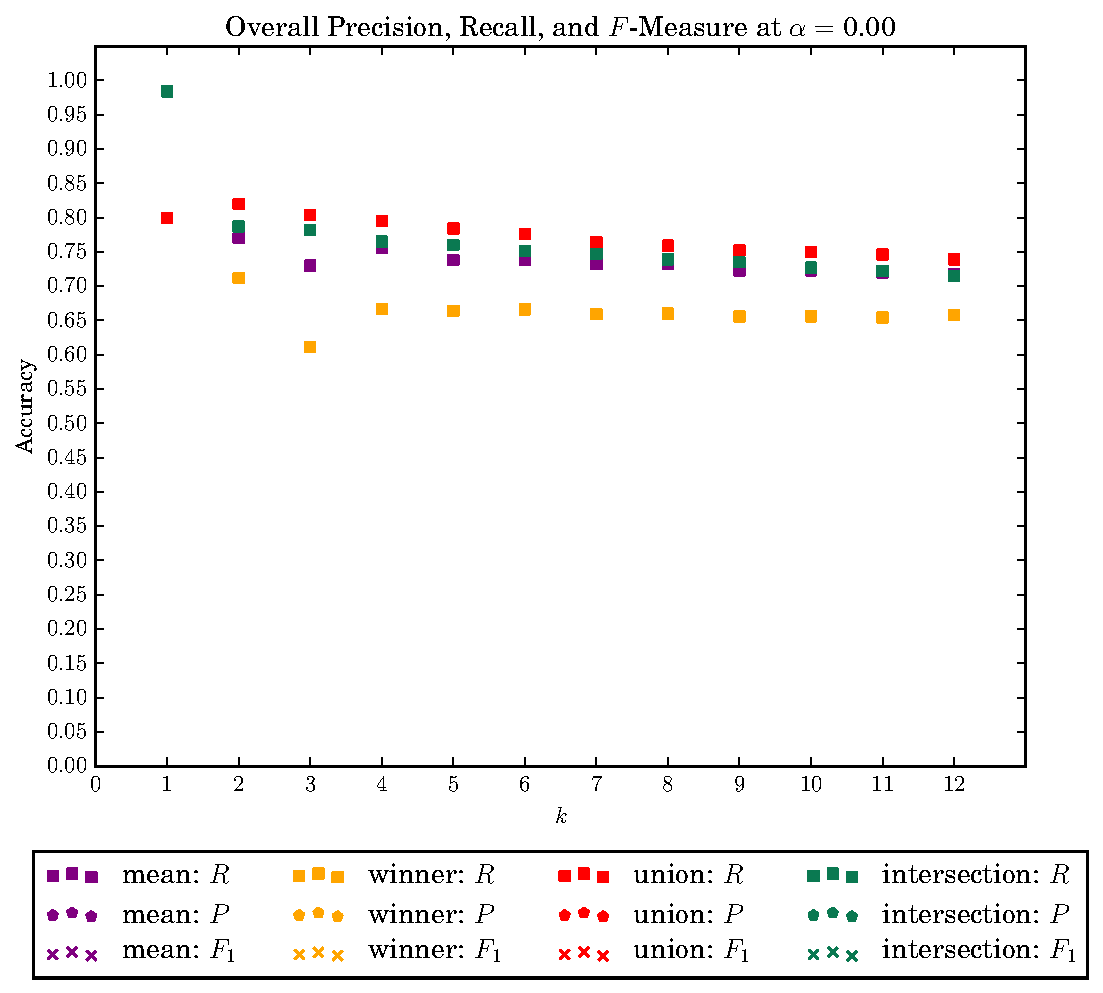
\includegraphics[width=3in]{figures/krap/Overall-ALL-metrics-12-0_000}
\krapfigure{figures/krap/Overall-ALL-metrics-12-0_000_new}
\caption{The accuracy  of all classifications performed with CPLOP across the four different algorithms with $\alpha=0.00$ shows little improvement for $k>5$. We look at only the percentage of correct classifications, since that value is equivalent to the precision and the recall.}
\label{fig:k_overall}
\end{figure}
Overall, for $k\geq5$, the accuracy does not improve, but instead levels off. Depending on the resolution algorithm, this value is between 65\% and 75\% accuracy, as shown in Figure \ref{fig:k_overall}. By ``overall,'' we mean that for every classification, we validated if it was correct and calculated what proportion to all classifications made that represents to determine accuracy. When looking at all classifications, precision and recall are identical values, as is $F$-measure.


\begin{figure}[t]
\centering
\krapfigure{figures/krap/Cow-ALL-metrics-12-0_000}
\caption{There are 1838 Cow \isol{}s in CPLOP. For most resolution algorithms, we observe little improvement when $k>5$.}
\label{fig:k_cow}
\end{figure}
One good example is the Cow. As Figure \ref{fig:k_cow} shows, Cow follows a trend similar to the overall accuracy, staying roughly between 70\% and 95\% accurate. Certain algorithms get worse for $k>5$, while other improve.

\begin{figure}[t]
\centering
\krapfigure{figures/krap/Cow-ALL-pvr-12-0_000}
\caption{There are 1838 Cow \isol{}s in CPLOP. Looking at the Recall as it compares to the Precision for $\alpha=0.99$ allows us to visualize the tradeoffs we make when picking a $k$ value. Labeled within each datapoint is the $k$ value at that point}
\label{fig:k_cow_pvr}
\end{figure}
Figure \ref{fig:k_cow_pvr} examines the relationship between $R$ and $P$. This can help us understand the trade offs of choosing one $k$ over another. We will later build a meaningful strategy for how confident we are at recalling a species versus our confidence in a classification of a species.


%ALPHA
\subsection{Adjusting \a{}}
By adding a threshold value, we investigated whether this further limitation improves the accuracy by restricting outliers from populating a \knn{} list. We investigate $\alpha = \{0.00,0.98,0.99\}$. Outside of this study, $\alpha = 0.99$ defines the boundary between strains. One reason we investigate 0.98 is to see whether loosening our definition of strain differentiation gives us a better accuracy.

\begin{figure}[t]
\centering
\krapfigure{figures/krap/Overall-ALL-metrics-12-[-0_----0_98--0_99]}
\caption{Shown is the accuracy of all classifications performed with CPLOP across the four different algorithms. We find that the accuracy of certain resolution algorithms perform better with higher $\alpha$ values.}
\label{fig:alpha_overall}
\end{figure}

Overall, we observe that the accuracy slightly improves as we increase the $\alpha$ threshold. Figure \ref{fig:alpha_overall} shows that overall, the accuracy increases as we increase $\alpha$. 

%\begin{figure}[t]
%\centering
%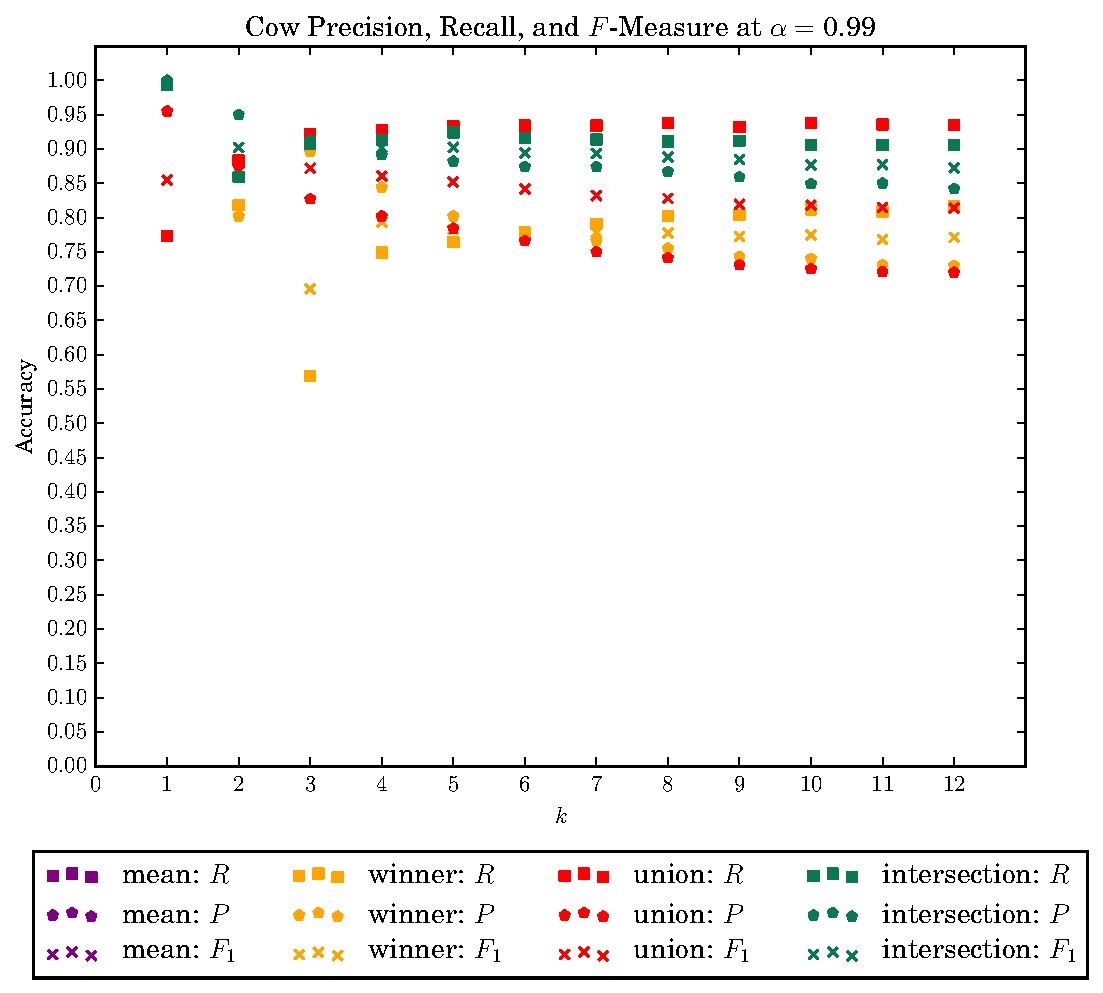
\includegraphics[width=3in]{figures/krap/Cow-ALL-metrics-12-0_990}
%\caption{There are 40 Chicken \isol{}s in CPLOP.}
%\label{fig:alpha_cow}
%\end{figure}

\begin{figure}[t]
\centering
\krapfigure{figures/krap/Cow-ALL-pvr-12-0_990}
\caption{There are 1838 Cow \isol{}s in CPLOP. Increasing the $\alpha$ for a species with this many \isol{}s made minimal improvements to the accuracy on all but the resolution by intersection algorithm, which, when compared to Figure \ref{fig:k_cow_pvr} noticeably improved.}
\label{fig:alpha_cow_pvr}
\end{figure}

Adding the $\alpha$ made minimal changes to the accuracy of Cow classifications, so only the recall versus precision is shown in Figure \ref{fig:alpha_cow_pvr}. More details into how $\alpha$ affect the classification accuracy can be seen in Tables \ref{tab:profile000}, \ref{tab:profile098}, and \ref{tab:profile099}.

%ALGORITHM
\subsection{Adjusting the Algorithm}
Choosing which algorithm to resolve the two different regions of each \isol{} is an important step. We investigate the differences between the aforementioned four algorithms as they relate to $k$ and $\alpha$ values and how each differ among species of different representation. With library-based-MST, it is important to realize the representation of a species in the library may heavily skew the accuracy of the library.

While interpreting the data, we state that there may be some ``\%'' increase or decrease which we intend to mean the increase in the raw value of the percentage.
Additionally, values in the tables represent the proportion of the three metrics, but are easily interpreted as percentages.
\autoref{sec:evaluation:krap} explains the meaning of each precision ($P$), recall ($R$), and $F$-measure ($F_1$).

\input{data/krap/tab_profile000}
Overall, with $\alpha=0.00$, Figure \ref{fig:k_overall} illustrates that the resolution by union algorithm consistently performs better. For $k=7$ and $\alpha = 0.00$, Table \ref{tab:profile000} shows that using the resolution by unions algorithm performs with 76.4\% accuracy with meanwise and resolution by winner and intersection respectively achieving 73.2\%, 65.9\%, and 74.7 accuracy\%.
Poorly represented species, like the Cat, Chicken, and Seagull did not benefit from the resolution by union algorithm, each achieving no classifications, correct or otherwise.

\input{data/krap/tab_profile098}
Once we restrict with a somewhat loose threshold of 0.98, overall we see that the intersection method provides the best accuracy, improving on non-thresholded values. For $k=7$ and $\alpha=0.98$, the intersection algorithm achieves 78.0\% accuracy, while resolution by winner and union respectively achieve 66.4\% and 76.7\% accuracy.

Table \ref{tab:profile098} shows that a handful of poorly represented species achieved slightly better results when $\alpha=0.98$. Notably, the intersection algorithm $F$-measure increased slightly for Wild Turkey, Cat, and Chicken on the order of 3\%.

Unfortunately, the meanwise algorithm fails to classify when we use a large enough $\alpha$ and thus we have ommited the results in Tables \ref{tab:profile098} and \ref{tab:profile099}. In certain cells of the tables, including Table \ref{tab:profile000}, empty values in either $P$ or $F_1$ mean no classifications were made of that species.



\input{data/krap/tab_profile099}
Restricting with $\alpha=0.99$, our definition of strain differentiation, overall accuracy improves more with resolution by intersection and less so with resolutions by winner and union, garnering 85.9\%, 68.0\%, and 76.6\% accuracy respectively. Again, meanwise resolution fails to produce any classifications.

For poorly represented species, we see some similar improvements for $P$, $R$, and $F_1$, but also some exceptions. Wild Turkey for example, improves by about 2\%-3\% for resolutions by winner and union and 11\% for resolution by intersection, while Cat decreases by 3\% for resolution by winner, but improves by 6\% and 47\% for resolution by union and intersection.

\subsection{Underrepresented Species}
\begin{figure}[t]
\centering
\krapfigure{figures/krap/Chicken-ALL-metrics-12-0_000}
\caption{There are 40 Chicken \isol{}s in CPLOP. Unfortunately, due to their low representation in CPLOP, classification accuracy is low.}
\label{fig:k_chicken}
\end{figure}
Some species had worse accuracy than the overall accuracy. In particular, species such as Chicken with only 40 \isol{}s representing it showed similar leveling of accuracy for $k>5$, but had far poorer accuracy, as shown in Figure \ref{fig:k_chicken}. For $k>5$, the accuracy of classifying chicken ranges from as low as 10\% to a peak of 26\%. The classification accuracy for many species in CPLOP heavily relies on its representation in CPLOP.

One notable exception is the Bat. In everyone application of our \kNN{} algorithms, Bat has above 95\% accuracy. It is possible that due to their small size and relative dietary segregation from the surrounding environment that the strains of \ecoli{} stay particularly unique. It may also be a quirk of the fact that each \isol{} comes from a single \host{}, making it difficult to draw conclusions from such results.


%%%%% DISCUSSION %%%%%
\section{Discussion}\label{sec:discussion:krap}
\chapter{Implementation}
\section{Resolution Algorithms}
\section{Graphing Results}
%\chapter{Evaluation}\label{chap:evaluation}
\section{Cluster Purity}
\section{Classification Metrics}
%\chapter{Results}\label{chap:results}
\section{Clustering}\label{sec:clusteringbsresults}
\section{Classifying}
\chapter{Conclusion}\label{chap:conclusion}

%%%%%%%%%% GLOSSARY
\printglossaries

%%%%%%%%%% INDEX
\clearpage
\phantomsection
%\addcontentsline{toc}{chapter}{Index}
\printindex

%%%%%%%%%% BIBLIOGRAPHY
\nocite{*}
\bibliography{bibliography}


%%%%%%%%%% APPENDICES
% Indents Appendix in Table of Contents
\makeatletter
\addtocontents{toc}{\let\protect\l@chapter\protect\l@section}
\makeatother

% Hack to make Appendices to appear in Table of Contents
\addtocontents{toc}{%
   \noindent APPENDICES
}
\begin{appendices}
\chapter{Cluster Counts}
Below are the \spec{} counts of each cluster for the clustering performed.

\let\svaddcontentsline\addcontentsline
\renewcommand\addcontentsline[3]{%
  \ifthenelse{\equal{#1}{lof}}{}%
  {\ifthenelse{\equal{#1}{lot}}{}{\svaddcontentsline{#1}{#2}{#3}}}}

\section{Cluster Counts for \minneigh{} = 1}
%%%%% CLUSTER 1 of 380 NEIGHBORS = 1 %%%%%
\begin{table}[ht!]
\centering
\begin{tabular}{|c|c|c|}
\hline
\bf \Spec{} &\bf Count &\bf Proportion\\ \hline \hline
Human & 168 & 0.468\\ \hline
Cow & 166 & 0.462\\ \hline
Pig & 7 & 0.019\\ \hline
Pigeon & 5 & 0.014\\ \hline
Sheep & 3 & 0.008\\ \hline
Ground Squirrel & 3 & 0.008\\ \hline
Chicken & 3 & 0.008\\ \hline
Dog & 2 & 0.006\\ \hline
Horse & 1 & 0.003\\ \hline
Coyote & 1 & 0.003\\ \hline
\hline
\bf Total & \bf 359 & \bf 1.000\\ \hline
\end{tabular}
\label{tab:cluster:1:1}
\caption{Cluster 1 of 380 for \minneigh{}=1}
\end{table}

%%%%% CLUSTER 2 of 380 NEIGHBORS = 1 %%%%%
\begin{table}[ht!]
\centering
\begin{tabular}{|c|c|c|}
\hline
\bf \Spec{} &\bf Count &\bf Proportion\\ \hline \hline
Human & 248 & 1.000\\ \hline
\hline
\bf Total & \bf 248 & \bf 1.000\\ \hline
\end{tabular}
\label{tab:cluster:2:1}
\caption{Cluster 2 of 380 for \minneigh{}=1}
\end{table}

%%%%% CLUSTER 3 of 380 NEIGHBORS = 1 %%%%%
\begin{table}[ht!]
\centering
\begin{tabular}{|c|c|c|}
\hline
\bf \Spec{} &\bf Count &\bf Proportion\\ \hline \hline
Cow & 163 & 0.734\\ \hline
Pigeon & 12 & 0.054\\ \hline
Dog & 10 & 0.045\\ \hline
Human & 8 & 0.036\\ \hline
Wild Turkey & 8 & 0.036\\ \hline
Ground Squirrel & 5 & 0.023\\ \hline
Cliff Sparrow & 4 & 0.018\\ \hline
Horse & 3 & 0.014\\ \hline
Chicken & 3 & 0.014\\ \hline
Sheep & 2 & 0.009\\ \hline
Turkey Vulture & 1 & 0.005\\ \hline
Pelican & 1 & 0.005\\ \hline
Deer Mouse & 1 & 0.005\\ \hline
Pig & 1 & 0.005\\ \hline
\hline
\bf Total & \bf 222 & \bf 1.000\\ \hline
\end{tabular}
\label{tab:cluster:3:1}
\caption{Cluster 3 of 380 for \minneigh{}=1}
\end{table}

%%%%% CLUSTER 4 of 380 NEIGHBORS = 1 %%%%%
\begin{table}[ht!]
\centering
\begin{tabular}{|c|c|c|}
\hline
\bf \Spec{} &\bf Count &\bf Proportion\\ \hline \hline
Human & 199 & 1.000\\ \hline
\hline
\bf Total & \bf 199 & \bf 1.000\\ \hline
\end{tabular}
\label{tab:cluster:4:1}
\caption{Cluster 4 of 380 for \minneigh{}=1}
\end{table}

%%%%% CLUSTER 5 of 380 NEIGHBORS = 1 %%%%%
\begin{table}[ht!]
\centering
\begin{tabular}{|c|c|c|}
\hline
\bf \Spec{} &\bf Count &\bf Proportion\\ \hline \hline
Human & 161 & 0.843\\ \hline
Cow & 15 & 0.079\\ \hline
Mountain Lion & 8 & 0.042\\ \hline
Deer & 6 & 0.031\\ \hline
Horse & 1 & 0.005\\ \hline
\hline
\bf Total & \bf 191 & \bf 1.000\\ \hline
\end{tabular}
\label{tab:cluster:5:1}
\caption{Cluster 5 of 380 for \minneigh{}=1}
\end{table}

%%%%% CLUSTER 6 of 380 NEIGHBORS = 1 %%%%%
\begin{table}[ht!]
\centering
\begin{tabular}{|c|c|c|}
\hline
\bf \Spec{} &\bf Count &\bf Proportion\\ \hline \hline
Human & 101 & 0.962\\ \hline
Coyote & 2 & 0.019\\ \hline
Mountain Lion & 2 & 0.019\\ \hline
\hline
\bf Total & \bf 105 & \bf 1.000\\ \hline
\end{tabular}
\label{tab:cluster:6:1}
\caption{Cluster 6 of 380 for \minneigh{}=1}
\end{table}

%%%%% CLUSTER 7 of 380 NEIGHBORS = 1 %%%%%
\begin{table}[ht!]
\centering
\begin{tabular}{|c|c|c|}
\hline
\bf \Spec{} &\bf Count &\bf Proportion\\ \hline \hline
Human & 76 & 0.760\\ \hline
Dog & 8 & 0.080\\ \hline
Ground Squirrel & 5 & 0.050\\ \hline
Grey Fox & 4 & 0.040\\ \hline
Mountain Lion & 2 & 0.020\\ \hline
Pigeon & 2 & 0.020\\ \hline
Cat & 1 & 0.010\\ \hline
Coyote & 1 & 0.010\\ \hline
Orangutan & 1 & 0.010\\ \hline
\hline
\bf Total & \bf 100 & \bf 1.000\\ \hline
\end{tabular}
\label{tab:cluster:7:1}
\caption{Cluster 7 of 380 for \minneigh{}=1}
\end{table}

%%%%% CLUSTER 8 of 380 NEIGHBORS = 1 %%%%%
\begin{table}[ht!]
\centering
\begin{tabular}{|c|c|c|}
\hline
\bf \Spec{} &\bf Count &\bf Proportion\\ \hline \hline
Human & 99 & 1.000\\ \hline
\hline
\bf Total & \bf 99 & \bf 1.000\\ \hline
\end{tabular}
\label{tab:cluster:8:1}
\caption{Cluster 8 of 380 for \minneigh{}=1}
\end{table}

%%%%% CLUSTER 9 of 380 NEIGHBORS = 1 %%%%%
\begin{table}[ht!]
\centering
\begin{tabular}{|c|c|c|}
\hline
\bf \Spec{} &\bf Count &\bf Proportion\\ \hline \hline
Human & 50 & 0.526\\ \hline
Cow & 41 & 0.432\\ \hline
Cliff Sparrow & 3 & 0.032\\ \hline
Pigeon & 1 & 0.011\\ \hline
\hline
\bf Total & \bf 95 & \bf 1.000\\ \hline
\end{tabular}
\label{tab:cluster:9:1}
\caption{Cluster 9 of 380 for \minneigh{}=1}
\end{table}

\clearpage
%%%%% CLUSTER 10 of 380 NEIGHBORS = 1 %%%%%
\begin{table}[ht!]
\centering
\begin{tabular}{|c|c|c|}
\hline
\bf \Spec{} &\bf Count &\bf Proportion\\ \hline \hline
Cow & 53 & 0.883\\ \hline
Sheep & 3 & 0.050\\ \hline
Cliff Sparrow & 2 & 0.033\\ \hline
Cat & 2 & 0.033\\ \hline
\hline
\bf Total & \bf 60 & \bf 1.000\\ \hline
\end{tabular}
\label{tab:cluster:10:1}
\caption{Cluster 10 of 380 for \minneigh{}=1}
\end{table}

%%%%% CLUSTER 11 of 380 NEIGHBORS = 1 %%%%%
\begin{table}[ht!]
\centering
\begin{tabular}{|c|c|c|}
\hline
\bf \Spec{} &\bf Count &\bf Proportion\\ \hline \hline
Human & 49 & 0.980\\ \hline
Cow & 1 & 0.020\\ \hline
\hline
\bf Total & \bf 50 & \bf 1.000\\ \hline
\end{tabular}
\label{tab:cluster:11:1}
\caption{Cluster 11 of 380 for \minneigh{}=1}
\end{table}

%%%%% CLUSTER 12 of 380 NEIGHBORS = 1 %%%%%
\begin{table}[ht!]
\centering
\begin{tabular}{|c|c|c|}
\hline
\bf \Spec{} &\bf Count &\bf Proportion\\ \hline \hline
Dog & 48 & 1.000\\ \hline
\hline
\bf Total & \bf 48 & \bf 1.000\\ \hline
\end{tabular}
\label{tab:cluster:12:1}
\caption{Cluster 12 of 380 for \minneigh{}=1}
\end{table}

%%%%% CLUSTER 13 of 380 NEIGHBORS = 1 %%%%%
\begin{table}[ht!]
\centering
\begin{tabular}{|c|c|c|}
\hline
\bf \Spec{} &\bf Count &\bf Proportion\\ \hline \hline
Bat & 36 & 0.837\\ \hline
Cow & 6 & 0.140\\ \hline
Human & 1 & 0.023\\ \hline
\hline
\bf Total & \bf 43 & \bf 1.000\\ \hline
\end{tabular}
\label{tab:cluster:13:1}
\caption{Cluster 13 of 380 for \minneigh{}=1}
\end{table}

%%%%% CLUSTER 14 of 380 NEIGHBORS = 1 %%%%%
\begin{table}[ht!]
\centering
\begin{tabular}{|c|c|c|}
\hline
\bf \Spec{} &\bf Count &\bf Proportion\\ \hline \hline
Cow & 41 & 1.000\\ \hline
\hline
\bf Total & \bf 41 & \bf 1.000\\ \hline
\end{tabular}
\label{tab:cluster:14:1}
\caption{Cluster 14 of 380 for \minneigh{}=1}
\end{table}

%%%%% CLUSTER 15 of 380 NEIGHBORS = 1 %%%%%
\begin{table}[ht!]
\centering
\begin{tabular}{|c|c|c|}
\hline
\bf \Spec{} &\bf Count &\bf Proportion\\ \hline \hline
Cow & 23 & 0.575\\ \hline
Sheep & 11 & 0.275\\ \hline
Pig & 3 & 0.075\\ \hline
Seagull & 1 & 0.025\\ \hline
Mallard Duck & 1 & 0.025\\ \hline
Western Kingbird & 1 & 0.025\\ \hline
\hline
\bf Total & \bf 40 & \bf 1.000\\ \hline
\end{tabular}
\label{tab:cluster:15:1}
\caption{Cluster 15 of 380 for \minneigh{}=1}
\end{table}

%%%%% CLUSTER 16 of 380 NEIGHBORS = 1 %%%%%
\begin{table}[ht!]
\centering
\begin{tabular}{|c|c|c|}
\hline
\bf \Spec{} &\bf Count &\bf Proportion\\ \hline \hline
Dog & 31 & 0.939\\ \hline
Wild Turkey & 2 & 0.061\\ \hline
\hline
\bf Total & \bf 33 & \bf 1.000\\ \hline
\end{tabular}
\label{tab:cluster:16:1}
\caption{Cluster 16 of 380 for \minneigh{}=1}
\end{table}

%%%%% CLUSTER 17 of 380 NEIGHBORS = 1 %%%%%
\begin{table}[ht!]
\centering
\begin{tabular}{|c|c|c|}
\hline
\bf \Spec{} &\bf Count &\bf Proportion\\ \hline \hline
Cow & 31 & 0.969\\ \hline
Wild Turkey & 1 & 0.031\\ \hline
\hline
\bf Total & \bf 32 & \bf 1.000\\ \hline
\end{tabular}
\label{tab:cluster:17:1}
\caption{Cluster 17 of 380 for \minneigh{}=1}
\end{table}

%%%%% CLUSTER 18 of 380 NEIGHBORS = 1 %%%%%
\begin{table}[ht!]
\centering
\begin{tabular}{|c|c|c|}
\hline
\bf \Spec{} &\bf Count &\bf Proportion\\ \hline \hline
Ground Squirrel & 18 & 0.621\\ \hline
Human & 2 & 0.069\\ \hline
Red-shoulder Hawk & 2 & 0.069\\ \hline
Great Horned Owl & 2 & 0.069\\ \hline
Horse & 2 & 0.069\\ \hline
Cow & 1 & 0.034\\ \hline
Red Shoulder Hawk & 1 & 0.034\\ \hline
Cat & 1 & 0.034\\ \hline
\hline
\bf Total & \bf 29 & \bf 1.000\\ \hline
\end{tabular}
\label{tab:cluster:18:1}
\caption{Cluster 18 of 380 for \minneigh{}=1}
\end{table}

%%%%% CLUSTER 19 of 380 NEIGHBORS = 1 %%%%%
\begin{table}[ht!]
\centering
\begin{tabular}{|c|c|c|}
\hline
\bf \Spec{} &\bf Count &\bf Proportion\\ \hline \hline
Sheep & 21 & 1.000\\ \hline
\hline
\bf Total & \bf 21 & \bf 1.000\\ \hline
\end{tabular}
\label{tab:cluster:19:1}
\caption{Cluster 19 of 380 for \minneigh{}=1}
\end{table}

\clearpage
%%%%% CLUSTER 20 of 380 NEIGHBORS = 1 %%%%%
\begin{table}[ht!]
\centering
\begin{tabular}{|c|c|c|}
\hline
\bf \Spec{} &\bf Count &\bf Proportion\\ \hline \hline
Human & 21 & 1.000\\ \hline
\hline
\bf Total & \bf 21 & \bf 1.000\\ \hline
\end{tabular}
\label{tab:cluster:20:1}
\caption{Cluster 20 of 380 for \minneigh{}=1}
\end{table}

%%%%% CLUSTER 21 of 380 NEIGHBORS = 1 %%%%%
\begin{table}[ht!]
\centering
\begin{tabular}{|c|c|c|}
\hline
\bf \Spec{} &\bf Count &\bf Proportion\\ \hline \hline
Human & 21 & 1.000\\ \hline
\hline
\bf Total & \bf 21 & \bf 1.000\\ \hline
\end{tabular}
\label{tab:cluster:21:1}
\caption{Cluster 21 of 380 for \minneigh{}=1}
\end{table}

%%%%% CLUSTER 22 of 380 NEIGHBORS = 1 %%%%%
\begin{table}[ht!]
\centering
\begin{tabular}{|c|c|c|}
\hline
\bf \Spec{} &\bf Count &\bf Proportion\\ \hline \hline
Human & 19 & 1.000\\ \hline
\hline
\bf Total & \bf 19 & \bf 1.000\\ \hline
\end{tabular}
\label{tab:cluster:22:1}
\caption{Cluster 22 of 380 for \minneigh{}=1}
\end{table}

%%%%% CLUSTER 23 of 380 NEIGHBORS = 1 %%%%%
\begin{table}[ht!]
\centering
\begin{tabular}{|c|c|c|}
\hline
\bf \Spec{} &\bf Count &\bf Proportion\\ \hline \hline
Cow & 18 & 0.947\\ \hline
Pigeon & 1 & 0.053\\ \hline
\hline
\bf Total & \bf 19 & \bf 1.000\\ \hline
\end{tabular}
\label{tab:cluster:23:1}
\caption{Cluster 23 of 380 for \minneigh{}=1}
\end{table}

%%%%% CLUSTER 24 of 380 NEIGHBORS = 1 %%%%%
\begin{table}[ht!]
\centering
\begin{tabular}{|c|c|c|}
\hline
\bf \Spec{} &\bf Count &\bf Proportion\\ \hline \hline
Sheep & 17 & 0.895\\ \hline
Chicken & 2 & 0.105\\ \hline
\hline
\bf Total & \bf 19 & \bf 1.000\\ \hline
\end{tabular}
\label{tab:cluster:24:1}
\caption{Cluster 24 of 380 for \minneigh{}=1}
\end{table}

%%%%% CLUSTER 25 of 380 NEIGHBORS = 1 %%%%%
\begin{table}[ht!]
\centering
\begin{tabular}{|c|c|c|}
\hline
\bf \Spec{} &\bf Count &\bf Proportion\\ \hline \hline
Cow & 18 & 1.000\\ \hline
\hline
\bf Total & \bf 18 & \bf 1.000\\ \hline
\end{tabular}
\label{tab:cluster:25:1}
\caption{Cluster 25 of 380 for \minneigh{}=1}
\end{table}

%%%%% CLUSTER 26 of 380 NEIGHBORS = 1 %%%%%
\begin{table}[ht!]
\centering
\begin{tabular}{|c|c|c|}
\hline
\bf \Spec{} &\bf Count &\bf Proportion\\ \hline \hline
Cow & 10 & 0.588\\ \hline
Ground Squirrel & 7 & 0.412\\ \hline
\hline
\bf Total & \bf 17 & \bf 1.000\\ \hline
\end{tabular}
\label{tab:cluster:26:1}
\caption{Cluster 26 of 380 for \minneigh{}=1}
\end{table}

%%%%% CLUSTER 27 of 380 NEIGHBORS = 1 %%%%%
\begin{table}[ht!]
\centering
\begin{tabular}{|c|c|c|}
\hline
\bf \Spec{} &\bf Count &\bf Proportion\\ \hline \hline
Cow & 16 & 1.000\\ \hline
\hline
\bf Total & \bf 16 & \bf 1.000\\ \hline
\end{tabular}
\label{tab:cluster:27:1}
\caption{Cluster 27 of 380 for \minneigh{}=1}
\end{table}

%%%%% CLUSTER 28 of 380 NEIGHBORS = 1 %%%%%
\begin{table}[ht!]
\centering
\begin{tabular}{|c|c|c|}
\hline
\bf \Spec{} &\bf Count &\bf Proportion\\ \hline \hline
Cow & 14 & 0.875\\ \hline
Ground Squirrel & 2 & 0.125\\ \hline
\hline
\bf Total & \bf 16 & \bf 1.000\\ \hline
\end{tabular}
\label{tab:cluster:28:1}
\caption{Cluster 28 of 380 for \minneigh{}=1}
\end{table}

%%%%% CLUSTER 29 of 380 NEIGHBORS = 1 %%%%%
\begin{table}[ht!]
\centering
\begin{tabular}{|c|c|c|}
\hline
\bf \Spec{} &\bf Count &\bf Proportion\\ \hline \hline
Human & 15 & 1.000\\ \hline
\hline
\bf Total & \bf 15 & \bf 1.000\\ \hline
\end{tabular}
\label{tab:cluster:29:1}
\caption{Cluster 29 of 380 for \minneigh{}=1}
\end{table}

\clearpage
%%%%% CLUSTER 30 of 380 NEIGHBORS = 1 %%%%%
\begin{table}[ht!]
\centering
\begin{tabular}{|c|c|c|}
\hline
\bf \Spec{} &\bf Count &\bf Proportion\\ \hline \hline
Human & 15 & 1.000\\ \hline
\hline
\bf Total & \bf 15 & \bf 1.000\\ \hline
\end{tabular}
\label{tab:cluster:30:1}
\caption{Cluster 30 of 380 for \minneigh{}=1}
\end{table}

%%%%% CLUSTER 31 of 380 NEIGHBORS = 1 %%%%%
\begin{table}[ht!]
\centering
\begin{tabular}{|c|c|c|}
\hline
\bf \Spec{} &\bf Count &\bf Proportion\\ \hline \hline
Cow & 14 & 1.000\\ \hline
\hline
\bf Total & \bf 14 & \bf 1.000\\ \hline
\end{tabular}
\label{tab:cluster:31:1}
\caption{Cluster 31 of 380 for \minneigh{}=1}
\end{table}

%%%%% CLUSTER 32 of 380 NEIGHBORS = 1 %%%%%
\begin{table}[ht!]
\centering
\begin{tabular}{|c|c|c|}
\hline
\bf \Spec{} &\bf Count &\bf Proportion\\ \hline \hline
Cow & 8 & 0.571\\ \hline
Wild Turkey & 6 & 0.429\\ \hline
\hline
\bf Total & \bf 14 & \bf 1.000\\ \hline
\end{tabular}
\label{tab:cluster:32:1}
\caption{Cluster 32 of 380 for \minneigh{}=1}
\end{table}

%%%%% CLUSTER 33 of 380 NEIGHBORS = 1 %%%%%
\begin{table}[ht!]
\centering
\begin{tabular}{|c|c|c|}
\hline
\bf \Spec{} &\bf Count &\bf Proportion\\ \hline \hline
Cow & 13 & 1.000\\ \hline
\hline
\bf Total & \bf 13 & \bf 1.000\\ \hline
\end{tabular}
\label{tab:cluster:33:1}
\caption{Cluster 33 of 380 for \minneigh{}=1}
\end{table}

%%%%% CLUSTER 34 of 380 NEIGHBORS = 1 %%%%%
\begin{table}[ht!]
\centering
\begin{tabular}{|c|c|c|}
\hline
\bf \Spec{} &\bf Count &\bf Proportion\\ \hline \hline
Cow & 12 & 1.000\\ \hline
\hline
\bf Total & \bf 12 & \bf 1.000\\ \hline
\end{tabular}
\label{tab:cluster:34:1}
\caption{Cluster 34 of 380 for \minneigh{}=1}
\end{table}

%%%%% CLUSTER 35 of 380 NEIGHBORS = 1 %%%%%
\begin{table}[ht!]
\centering
\begin{tabular}{|c|c|c|}
\hline
\bf \Spec{} &\bf Count &\bf Proportion\\ \hline \hline
Cow & 12 & 1.000\\ \hline
\hline
\bf Total & \bf 12 & \bf 1.000\\ \hline
\end{tabular}
\label{tab:cluster:35:1}
\caption{Cluster 35 of 380 for \minneigh{}=1}
\end{table}

%%%%% CLUSTER 36 of 380 NEIGHBORS = 1 %%%%%
\begin{table}[ht!]
\centering
\begin{tabular}{|c|c|c|}
\hline
\bf \Spec{} &\bf Count &\bf Proportion\\ \hline \hline
Cow & 12 & 1.000\\ \hline
\hline
\bf Total & \bf 12 & \bf 1.000\\ \hline
\end{tabular}
\label{tab:cluster:36:1}
\caption{Cluster 36 of 380 for \minneigh{}=1}
\end{table}

%%%%% CLUSTER 37 of 380 NEIGHBORS = 1 %%%%%
\begin{table}[ht!]
\centering
\begin{tabular}{|c|c|c|}
\hline
\bf \Spec{} &\bf Count &\bf Proportion\\ \hline \hline
Ground Squirrel & 12 & 1.000\\ \hline
\hline
\bf Total & \bf 12 & \bf 1.000\\ \hline
\end{tabular}
\label{tab:cluster:37:1}
\caption{Cluster 37 of 380 for \minneigh{}=1}
\end{table}

%%%%% CLUSTER 38 of 380 NEIGHBORS = 1 %%%%%
\begin{table}[ht!]
\centering
\begin{tabular}{|c|c|c|}
\hline
\bf \Spec{} &\bf Count &\bf Proportion\\ \hline \hline
Cow & 10 & 0.909\\ \hline
Ground Squirrel & 1 & 0.091\\ \hline
\hline
\bf Total & \bf 11 & \bf 1.000\\ \hline
\end{tabular}
\label{tab:cluster:38:1}
\caption{Cluster 38 of 380 for \minneigh{}=1}
\end{table}

%%%%% CLUSTER 39 of 380 NEIGHBORS = 1 %%%%%
\begin{table}[ht!]
\centering
\begin{tabular}{|c|c|c|}
\hline
\bf \Spec{} &\bf Count &\bf Proportion\\ \hline \hline
Cow & 4 & 0.364\\ \hline
Wild Turkey & 3 & 0.273\\ \hline
Red-Winged Blackbird & 2 & 0.182\\ \hline
Pigeon & 1 & 0.091\\ \hline
Pig & 1 & 0.091\\ \hline
\hline
\bf Total & \bf 11 & \bf 1.000\\ \hline
\end{tabular}
\label{tab:cluster:39:1}
\caption{Cluster 39 of 380 for \minneigh{}=1}
\end{table}

\clearpage
%%%%% CLUSTER 40 of 380 NEIGHBORS = 1 %%%%%
\begin{table}[ht!]
\centering
\begin{tabular}{|c|c|c|}
\hline
\bf \Spec{} &\bf Count &\bf Proportion\\ \hline \hline
Human & 3 & 0.273\\ \hline
Wild Turkey & 2 & 0.182\\ \hline
Elephant Seal & 2 & 0.182\\ \hline
California Sea Lion & 2 & 0.182\\ \hline
Sea Lion & 2 & 0.182\\ \hline
\hline
\bf Total & \bf 11 & \bf 1.000\\ \hline
\end{tabular}
\label{tab:cluster:40:1}
\caption{Cluster 40 of 380 for \minneigh{}=1}
\end{table}

%%%%% CLUSTER 41 of 380 NEIGHBORS = 1 %%%%%
\begin{table}[ht!]
\centering
\begin{tabular}{|c|c|c|}
\hline
\bf \Spec{} &\bf Count &\bf Proportion\\ \hline \hline
Human & 11 & 1.000\\ \hline
\hline
\bf Total & \bf 11 & \bf 1.000\\ \hline
\end{tabular}
\label{tab:cluster:41:1}
\caption{Cluster 41 of 380 for \minneigh{}=1}
\end{table}

%%%%% CLUSTER 42 of 380 NEIGHBORS = 1 %%%%%
\begin{table}[ht!]
\centering
\begin{tabular}{|c|c|c|}
\hline
\bf \Spec{} &\bf Count &\bf Proportion\\ \hline \hline
Deer & 10 & 1.000\\ \hline
\hline
\bf Total & \bf 10 & \bf 1.000\\ \hline
\end{tabular}
\label{tab:cluster:42:1}
\caption{Cluster 42 of 380 for \minneigh{}=1}
\end{table}

%%%%% CLUSTER 43 of 380 NEIGHBORS = 1 %%%%%
\begin{table}[ht!]
\centering
\begin{tabular}{|c|c|c|}
\hline
\bf \Spec{} &\bf Count &\bf Proportion\\ \hline \hline
Cow & 9 & 1.000\\ \hline
\hline
\bf Total & \bf 9 & \bf 1.000\\ \hline
\end{tabular}
\label{tab:cluster:43:1}
\caption{Cluster 43 of 380 for \minneigh{}=1}
\end{table}

%%%%% CLUSTER 44 of 380 NEIGHBORS = 1 %%%%%
\begin{table}[ht!]
\centering
\begin{tabular}{|c|c|c|}
\hline
\bf \Spec{} &\bf Count &\bf Proportion\\ \hline \hline
Pelican & 4 & 0.444\\ \hline
Red Throated Loon & 2 & 0.222\\ \hline
Common Loon & 2 & 0.222\\ \hline
Common Murre & 1 & 0.111\\ \hline
\hline
\bf Total & \bf 9 & \bf 1.000\\ \hline
\end{tabular}
\label{tab:cluster:44:1}
\caption{Cluster 44 of 380 for \minneigh{}=1}
\end{table}

%%%%% CLUSTER 45 of 380 NEIGHBORS = 1 %%%%%
\begin{table}[ht!]
\centering
\begin{tabular}{|c|c|c|}
\hline
\bf \Spec{} &\bf Count &\bf Proportion\\ \hline \hline
Cow & 9 & 1.000\\ \hline
\hline
\bf Total & \bf 9 & \bf 1.000\\ \hline
\end{tabular}
\label{tab:cluster:45:1}
\caption{Cluster 45 of 380 for \minneigh{}=1}
\end{table}

%%%%% CLUSTER 46 of 380 NEIGHBORS = 1 %%%%%
\begin{table}[ht!]
\centering
\begin{tabular}{|c|c|c|}
\hline
\bf \Spec{} &\bf Count &\bf Proportion\\ \hline \hline
Ground Squirrel & 9 & 1.000\\ \hline
\hline
\bf Total & \bf 9 & \bf 1.000\\ \hline
\end{tabular}
\label{tab:cluster:46:1}
\caption{Cluster 46 of 380 for \minneigh{}=1}
\end{table}

%%%%% CLUSTER 47 of 380 NEIGHBORS = 1 %%%%%
\begin{table}[ht!]
\centering
\begin{tabular}{|c|c|c|}
\hline
\bf \Spec{} &\bf Count &\bf Proportion\\ \hline \hline
Pigeon & 5 & 0.625\\ \hline
Cliff Sparrow & 3 & 0.375\\ \hline
\hline
\bf Total & \bf 8 & \bf 1.000\\ \hline
\end{tabular}
\label{tab:cluster:47:1}
\caption{Cluster 47 of 380 for \minneigh{}=1}
\end{table}

%%%%% CLUSTER 48 of 380 NEIGHBORS = 1 %%%%%
\begin{table}[ht!]
\centering
\begin{tabular}{|c|c|c|}
\hline
\bf \Spec{} &\bf Count &\bf Proportion\\ \hline \hline
Cat & 8 & 1.000\\ \hline
\hline
\bf Total & \bf 8 & \bf 1.000\\ \hline
\end{tabular}
\label{tab:cluster:48:1}
\caption{Cluster 48 of 380 for \minneigh{}=1}
\end{table}

%%%%% CLUSTER 49 of 380 NEIGHBORS = 1 %%%%%
\begin{table}[ht!]
\centering
\begin{tabular}{|c|c|c|}
\hline
\bf \Spec{} &\bf Count &\bf Proportion\\ \hline \hline
Sea Otter & 8 & 1.000\\ \hline
\hline
\bf Total & \bf 8 & \bf 1.000\\ \hline
\end{tabular}
\label{tab:cluster:49:1}
\caption{Cluster 49 of 380 for \minneigh{}=1}
\end{table}

\clearpage
%%%%% CLUSTER 50 of 380 NEIGHBORS = 1 %%%%%
\begin{table}[ht!]
\centering
\begin{tabular}{|c|c|c|}
\hline
\bf \Spec{} &\bf Count &\bf Proportion\\ \hline \hline
Human & 7 & 0.875\\ \hline
Cow & 1 & 0.125\\ \hline
\hline
\bf Total & \bf 8 & \bf 1.000\\ \hline
\end{tabular}
\label{tab:cluster:50:1}
\caption{Cluster 50 of 380 for \minneigh{}=1}
\end{table}

%%%%% CLUSTER 51 of 380 NEIGHBORS = 1 %%%%%
\begin{table}[ht!]
\centering
\begin{tabular}{|c|c|c|}
\hline
\bf \Spec{} &\bf Count &\bf Proportion\\ \hline \hline
Cow & 8 & 1.000\\ \hline
\hline
\bf Total & \bf 8 & \bf 1.000\\ \hline
\end{tabular}
\label{tab:cluster:51:1}
\caption{Cluster 51 of 380 for \minneigh{}=1}
\end{table}

%%%%% CLUSTER 52 of 380 NEIGHBORS = 1 %%%%%
\begin{table}[ht!]
\centering
\begin{tabular}{|c|c|c|}
\hline
\bf \Spec{} &\bf Count &\bf Proportion\\ \hline \hline
Cow & 7 & 1.000\\ \hline
\hline
\bf Total & \bf 7 & \bf 1.000\\ \hline
\end{tabular}
\label{tab:cluster:52:1}
\caption{Cluster 52 of 380 for \minneigh{}=1}
\end{table}

%%%%% CLUSTER 53 of 380 NEIGHBORS = 1 %%%%%
\begin{table}[ht!]
\centering
\begin{tabular}{|c|c|c|}
\hline
\bf \Spec{} &\bf Count &\bf Proportion\\ \hline \hline
Ground Squirrel & 7 & 1.000\\ \hline
\hline
\bf Total & \bf 7 & \bf 1.000\\ \hline
\end{tabular}
\label{tab:cluster:53:1}
\caption{Cluster 53 of 380 for \minneigh{}=1}
\end{table}

%%%%% CLUSTER 54 of 380 NEIGHBORS = 1 %%%%%
\begin{table}[ht!]
\centering
\begin{tabular}{|c|c|c|}
\hline
\bf \Spec{} &\bf Count &\bf Proportion\\ \hline \hline
Cow & 7 & 1.000\\ \hline
\hline
\bf Total & \bf 7 & \bf 1.000\\ \hline
\end{tabular}
\label{tab:cluster:54:1}
\caption{Cluster 54 of 380 for \minneigh{}=1}
\end{table}

%%%%% CLUSTER 55 of 380 NEIGHBORS = 1 %%%%%
\begin{table}[ht!]
\centering
\begin{tabular}{|c|c|c|}
\hline
\bf \Spec{} &\bf Count &\bf Proportion\\ \hline \hline
Pigeon & 5 & 0.714\\ \hline
Pig & 2 & 0.286\\ \hline
\hline
\bf Total & \bf 7 & \bf 1.000\\ \hline
\end{tabular}
\label{tab:cluster:55:1}
\caption{Cluster 55 of 380 for \minneigh{}=1}
\end{table}

%%%%% CLUSTER 56 of 380 NEIGHBORS = 1 %%%%%
\begin{table}[ht!]
\centering
\begin{tabular}{|c|c|c|}
\hline
\bf \Spec{} &\bf Count &\bf Proportion\\ \hline \hline
Cow & 6 & 0.857\\ \hline
Wild Turkey & 1 & 0.143\\ \hline
\hline
\bf Total & \bf 7 & \bf 1.000\\ \hline
\end{tabular}
\label{tab:cluster:56:1}
\caption{Cluster 56 of 380 for \minneigh{}=1}
\end{table}

%%%%% CLUSTER 57 of 380 NEIGHBORS = 1 %%%%%
\begin{table}[ht!]
\centering
\begin{tabular}{|c|c|c|}
\hline
\bf \Spec{} &\bf Count &\bf Proportion\\ \hline \hline
Cow & 6 & 0.857\\ \hline
Chicken & 1 & 0.143\\ \hline
\hline
\bf Total & \bf 7 & \bf 1.000\\ \hline
\end{tabular}
\label{tab:cluster:57:1}
\caption{Cluster 57 of 380 for \minneigh{}=1}
\end{table}

%%%%% CLUSTER 58 of 380 NEIGHBORS = 1 %%%%%
\begin{table}[ht!]
\centering
\begin{tabular}{|c|c|c|}
\hline
\bf \Spec{} &\bf Count &\bf Proportion\\ \hline \hline
Human & 5 & 0.714\\ \hline
Ground Squirrel & 1 & 0.143\\ \hline
Pelican & 1 & 0.143\\ \hline
\hline
\bf Total & \bf 7 & \bf 1.000\\ \hline
\end{tabular}
\label{tab:cluster:58:1}
\caption{Cluster 58 of 380 for \minneigh{}=1}
\end{table}

%%%%% CLUSTER 59 of 380 NEIGHBORS = 1 %%%%%
\begin{table}[ht!]
\centering
\begin{tabular}{|c|c|c|}
\hline
\bf \Spec{} &\bf Count &\bf Proportion\\ \hline \hline
Ground Squirrel & 7 & 1.000\\ \hline
\hline
\bf Total & \bf 7 & \bf 1.000\\ \hline
\end{tabular}
\label{tab:cluster:59:1}
\caption{Cluster 59 of 380 for \minneigh{}=1}
\end{table}

\clearpage
%%%%% CLUSTER 60 of 380 NEIGHBORS = 1 %%%%%
\begin{table}[ht!]
\centering
\begin{tabular}{|c|c|c|}
\hline
\bf \Spec{} &\bf Count &\bf Proportion\\ \hline \hline
Cow & 7 & 1.000\\ \hline
\hline
\bf Total & \bf 7 & \bf 1.000\\ \hline
\end{tabular}
\label{tab:cluster:60:1}
\caption{Cluster 60 of 380 for \minneigh{}=1}
\end{table}

%%%%% CLUSTER 61 of 380 NEIGHBORS = 1 %%%%%
\begin{table}[ht!]
\centering
\begin{tabular}{|c|c|c|}
\hline
\bf \Spec{} &\bf Count &\bf Proportion\\ \hline \hline
Human & 5 & 0.833\\ \hline
Chicken & 1 & 0.167\\ \hline
\hline
\bf Total & \bf 6 & \bf 1.000\\ \hline
\end{tabular}
\label{tab:cluster:61:1}
\caption{Cluster 61 of 380 for \minneigh{}=1}
\end{table}

%%%%% CLUSTER 62 of 380 NEIGHBORS = 1 %%%%%
\begin{table}[ht!]
\centering
\begin{tabular}{|c|c|c|}
\hline
\bf \Spec{} &\bf Count &\bf Proportion\\ \hline \hline
Cow & 6 & 1.000\\ \hline
\hline
\bf Total & \bf 6 & \bf 1.000\\ \hline
\end{tabular}
\label{tab:cluster:62:1}
\caption{Cluster 62 of 380 for \minneigh{}=1}
\end{table}

%%%%% CLUSTER 63 of 380 NEIGHBORS = 1 %%%%%
\begin{table}[ht!]
\centering
\begin{tabular}{|c|c|c|}
\hline
\bf \Spec{} &\bf Count &\bf Proportion\\ \hline \hline
Bear & 5 & 0.833\\ \hline
Ground Squirrel & 1 & 0.167\\ \hline
\hline
\bf Total & \bf 6 & \bf 1.000\\ \hline
\end{tabular}
\label{tab:cluster:63:1}
\caption{Cluster 63 of 380 for \minneigh{}=1}
\end{table}

%%%%% CLUSTER 64 of 380 NEIGHBORS = 1 %%%%%
\begin{table}[ht!]
\centering
\begin{tabular}{|c|c|c|}
\hline
\bf \Spec{} &\bf Count &\bf Proportion\\ \hline \hline
Cow & 5 & 0.833\\ \hline
Wild Turkey & 1 & 0.167\\ \hline
\hline
\bf Total & \bf 6 & \bf 1.000\\ \hline
\end{tabular}
\label{tab:cluster:64:1}
\caption{Cluster 64 of 380 for \minneigh{}=1}
\end{table}

%%%%% CLUSTER 65 of 380 NEIGHBORS = 1 %%%%%
\begin{table}[ht!]
\centering
\begin{tabular}{|c|c|c|}
\hline
\bf \Spec{} &\bf Count &\bf Proportion\\ \hline \hline
Cow & 6 & 1.000\\ \hline
\hline
\bf Total & \bf 6 & \bf 1.000\\ \hline
\end{tabular}
\label{tab:cluster:65:1}
\caption{Cluster 65 of 380 for \minneigh{}=1}
\end{table}

%%%%% CLUSTER 66 of 380 NEIGHBORS = 1 %%%%%
\begin{table}[ht!]
\centering
\begin{tabular}{|c|c|c|}
\hline
\bf \Spec{} &\bf Count &\bf Proportion\\ \hline \hline
Ground Squirrel & 6 & 1.000\\ \hline
\hline
\bf Total & \bf 6 & \bf 1.000\\ \hline
\end{tabular}
\label{tab:cluster:66:1}
\caption{Cluster 66 of 380 for \minneigh{}=1}
\end{table}

%%%%% CLUSTER 67 of 380 NEIGHBORS = 1 %%%%%
\begin{table}[ht!]
\centering
\begin{tabular}{|c|c|c|}
\hline
\bf \Spec{} &\bf Count &\bf Proportion\\ \hline \hline
Pigeon & 6 & 1.000\\ \hline
\hline
\bf Total & \bf 6 & \bf 1.000\\ \hline
\end{tabular}
\label{tab:cluster:67:1}
\caption{Cluster 67 of 380 for \minneigh{}=1}
\end{table}

%%%%% CLUSTER 68 of 380 NEIGHBORS = 1 %%%%%
\begin{table}[ht!]
\centering
\begin{tabular}{|c|c|c|}
\hline
\bf \Spec{} &\bf Count &\bf Proportion\\ \hline \hline
Cow & 6 & 1.000\\ \hline
\hline
\bf Total & \bf 6 & \bf 1.000\\ \hline
\end{tabular}
\label{tab:cluster:68:1}
\caption{Cluster 68 of 380 for \minneigh{}=1}
\end{table}

%%%%% CLUSTER 69 of 380 NEIGHBORS = 1 %%%%%
\begin{table}[ht!]
\centering
\begin{tabular}{|c|c|c|}
\hline
\bf \Spec{} &\bf Count &\bf Proportion\\ \hline \hline
Human & 6 & 1.000\\ \hline
\hline
\bf Total & \bf 6 & \bf 1.000\\ \hline
\end{tabular}
\label{tab:cluster:69:1}
\caption{Cluster 69 of 380 for \minneigh{}=1}
\end{table}

\clearpage
%%%%% CLUSTER 70 of 380 NEIGHBORS = 1 %%%%%
\begin{table}[ht!]
\centering
\begin{tabular}{|c|c|c|}
\hline
\bf \Spec{} &\bf Count &\bf Proportion\\ \hline \hline
Mountain Lion & 6 & 1.000\\ \hline
\hline
\bf Total & \bf 6 & \bf 1.000\\ \hline
\end{tabular}
\label{tab:cluster:70:1}
\caption{Cluster 70 of 380 for \minneigh{}=1}
\end{table}

%%%%% CLUSTER 71 of 380 NEIGHBORS = 1 %%%%%
\begin{table}[ht!]
\centering
\begin{tabular}{|c|c|c|}
\hline
\bf \Spec{} &\bf Count &\bf Proportion\\ \hline \hline
Cow & 5 & 1.000\\ \hline
\hline
\bf Total & \bf 5 & \bf 1.000\\ \hline
\end{tabular}
\label{tab:cluster:71:1}
\caption{Cluster 71 of 380 for \minneigh{}=1}
\end{table}

%%%%% CLUSTER 72 of 380 NEIGHBORS = 1 %%%%%
\begin{table}[ht!]
\centering
\begin{tabular}{|c|c|c|}
\hline
\bf \Spec{} &\bf Count &\bf Proportion\\ \hline \hline
Cow & 5 & 1.000\\ \hline
\hline
\bf Total & \bf 5 & \bf 1.000\\ \hline
\end{tabular}
\label{tab:cluster:72:1}
\caption{Cluster 72 of 380 for \minneigh{}=1}
\end{table}

%%%%% CLUSTER 73 of 380 NEIGHBORS = 1 %%%%%
\begin{table}[ht!]
\centering
\begin{tabular}{|c|c|c|}
\hline
\bf \Spec{} &\bf Count &\bf Proportion\\ \hline \hline
Cow & 5 & 1.000\\ \hline
\hline
\bf Total & \bf 5 & \bf 1.000\\ \hline
\end{tabular}
\label{tab:cluster:73:1}
\caption{Cluster 73 of 380 for \minneigh{}=1}
\end{table}

%%%%% CLUSTER 74 of 380 NEIGHBORS = 1 %%%%%
\begin{table}[ht!]
\centering
\begin{tabular}{|c|c|c|}
\hline
\bf \Spec{} &\bf Count &\bf Proportion\\ \hline \hline
Cow & 5 & 1.000\\ \hline
\hline
\bf Total & \bf 5 & \bf 1.000\\ \hline
\end{tabular}
\label{tab:cluster:74:1}
\caption{Cluster 74 of 380 for \minneigh{}=1}
\end{table}

%%%%% CLUSTER 75 of 380 NEIGHBORS = 1 %%%%%
\begin{table}[ht!]
\centering
\begin{tabular}{|c|c|c|}
\hline
\bf \Spec{} &\bf Count &\bf Proportion\\ \hline \hline
Cow & 5 & 1.000\\ \hline
\hline
\bf Total & \bf 5 & \bf 1.000\\ \hline
\end{tabular}
\label{tab:cluster:75:1}
\caption{Cluster 75 of 380 for \minneigh{}=1}
\end{table}

%%%%% CLUSTER 76 of 380 NEIGHBORS = 1 %%%%%
\begin{table}[ht!]
\centering
\begin{tabular}{|c|c|c|}
\hline
\bf \Spec{} &\bf Count &\bf Proportion\\ \hline \hline
Pig & 2 & 0.400\\ \hline
Mountain Lion & 2 & 0.400\\ \hline
Human & 1 & 0.200\\ \hline
\hline
\bf Total & \bf 5 & \bf 1.000\\ \hline
\end{tabular}
\label{tab:cluster:76:1}
\caption{Cluster 76 of 380 for \minneigh{}=1}
\end{table}

%%%%% CLUSTER 77 of 380 NEIGHBORS = 1 %%%%%
\begin{table}[ht!]
\centering
\begin{tabular}{|c|c|c|}
\hline
\bf \Spec{} &\bf Count &\bf Proportion\\ \hline \hline
Pigeon & 5 & 1.000\\ \hline
\hline
\bf Total & \bf 5 & \bf 1.000\\ \hline
\end{tabular}
\label{tab:cluster:77:1}
\caption{Cluster 77 of 380 for \minneigh{}=1}
\end{table}

%%%%% CLUSTER 78 of 380 NEIGHBORS = 1 %%%%%
\begin{table}[ht!]
\centering
\begin{tabular}{|c|c|c|}
\hline
\bf \Spec{} &\bf Count &\bf Proportion\\ \hline \hline
Cow & 5 & 1.000\\ \hline
\hline
\bf Total & \bf 5 & \bf 1.000\\ \hline
\end{tabular}
\label{tab:cluster:78:1}
\caption{Cluster 78 of 380 for \minneigh{}=1}
\end{table}

%%%%% CLUSTER 79 of 380 NEIGHBORS = 1 %%%%%
\begin{table}[ht!]
\centering
\begin{tabular}{|c|c|c|}
\hline
\bf \Spec{} &\bf Count &\bf Proportion\\ \hline \hline
Cow & 5 & 1.000\\ \hline
\hline
\bf Total & \bf 5 & \bf 1.000\\ \hline
\end{tabular}
\label{tab:cluster:79:1}
\caption{Cluster 79 of 380 for \minneigh{}=1}
\end{table}

\clearpage
%%%%% CLUSTER 80 of 380 NEIGHBORS = 1 %%%%%
\begin{table}[ht!]
\centering
\begin{tabular}{|c|c|c|}
\hline
\bf \Spec{} &\bf Count &\bf Proportion\\ \hline \hline
Pigeon & 5 & 1.000\\ \hline
\hline
\bf Total & \bf 5 & \bf 1.000\\ \hline
\end{tabular}
\label{tab:cluster:80:1}
\caption{Cluster 80 of 380 for \minneigh{}=1}
\end{table}

%%%%% CLUSTER 81 of 380 NEIGHBORS = 1 %%%%%
\begin{table}[ht!]
\centering
\begin{tabular}{|c|c|c|}
\hline
\bf \Spec{} &\bf Count &\bf Proportion\\ \hline \hline
Cow & 5 & 1.000\\ \hline
\hline
\bf Total & \bf 5 & \bf 1.000\\ \hline
\end{tabular}
\label{tab:cluster:81:1}
\caption{Cluster 81 of 380 for \minneigh{}=1}
\end{table}

%%%%% CLUSTER 82 of 380 NEIGHBORS = 1 %%%%%
\begin{table}[ht!]
\centering
\begin{tabular}{|c|c|c|}
\hline
\bf \Spec{} &\bf Count &\bf Proportion\\ \hline \hline
Pig & 5 & 1.000\\ \hline
\hline
\bf Total & \bf 5 & \bf 1.000\\ \hline
\end{tabular}
\label{tab:cluster:82:1}
\caption{Cluster 82 of 380 for \minneigh{}=1}
\end{table}

%%%%% CLUSTER 83 of 380 NEIGHBORS = 1 %%%%%
\begin{table}[ht!]
\centering
\begin{tabular}{|c|c|c|}
\hline
\bf \Spec{} &\bf Count &\bf Proportion\\ \hline \hline
Cow & 5 & 1.000\\ \hline
\hline
\bf Total & \bf 5 & \bf 1.000\\ \hline
\end{tabular}
\label{tab:cluster:83:1}
\caption{Cluster 83 of 380 for \minneigh{}=1}
\end{table}

%%%%% CLUSTER 84 of 380 NEIGHBORS = 1 %%%%%
\begin{table}[ht!]
\centering
\begin{tabular}{|c|c|c|}
\hline
\bf \Spec{} &\bf Count &\bf Proportion\\ \hline \hline
Cow & 5 & 1.000\\ \hline
\hline
\bf Total & \bf 5 & \bf 1.000\\ \hline
\end{tabular}
\label{tab:cluster:84:1}
\caption{Cluster 84 of 380 for \minneigh{}=1}
\end{table}

%%%%% CLUSTER 85 of 380 NEIGHBORS = 1 %%%%%
\begin{table}[ht!]
\centering
\begin{tabular}{|c|c|c|}
\hline
\bf \Spec{} &\bf Count &\bf Proportion\\ \hline \hline
Cow & 5 & 1.000\\ \hline
\hline
\bf Total & \bf 5 & \bf 1.000\\ \hline
\end{tabular}
\label{tab:cluster:85:1}
\caption{Cluster 85 of 380 for \minneigh{}=1}
\end{table}

%%%%% CLUSTER 86 of 380 NEIGHBORS = 1 %%%%%
\begin{table}[ht!]
\centering
\begin{tabular}{|c|c|c|}
\hline
\bf \Spec{} &\bf Count &\bf Proportion\\ \hline \hline
Human & 5 & 1.000\\ \hline
\hline
\bf Total & \bf 5 & \bf 1.000\\ \hline
\end{tabular}
\label{tab:cluster:86:1}
\caption{Cluster 86 of 380 for \minneigh{}=1}
\end{table}

%%%%% CLUSTER 87 of 380 NEIGHBORS = 1 %%%%%
\begin{table}[ht!]
\centering
\begin{tabular}{|c|c|c|}
\hline
\bf \Spec{} &\bf Count &\bf Proportion\\ \hline \hline
Cow & 5 & 1.000\\ \hline
\hline
\bf Total & \bf 5 & \bf 1.000\\ \hline
\end{tabular}
\label{tab:cluster:87:1}
\caption{Cluster 87 of 380 for \minneigh{}=1}
\end{table}

%%%%% CLUSTER 88 of 380 NEIGHBORS = 1 %%%%%
\begin{table}[ht!]
\centering
\begin{tabular}{|c|c|c|}
\hline
\bf \Spec{} &\bf Count &\bf Proportion\\ \hline \hline
Cow & 4 & 1.000\\ \hline
\hline
\bf Total & \bf 4 & \bf 1.000\\ \hline
\end{tabular}
\label{tab:cluster:88:1}
\caption{Cluster 88 of 380 for \minneigh{}=1}
\end{table}

%%%%% CLUSTER 89 of 380 NEIGHBORS = 1 %%%%%
\begin{table}[ht!]
\centering
\begin{tabular}{|c|c|c|}
\hline
\bf \Spec{} &\bf Count &\bf Proportion\\ \hline \hline
Cow & 4 & 1.000\\ \hline
\hline
\bf Total & \bf 4 & \bf 1.000\\ \hline
\end{tabular}
\label{tab:cluster:89:1}
\caption{Cluster 89 of 380 for \minneigh{}=1}
\end{table}

\clearpage
%%%%% CLUSTER 90 of 380 NEIGHBORS = 1 %%%%%
\begin{table}[ht!]
\centering
\begin{tabular}{|c|c|c|}
\hline
\bf \Spec{} &\bf Count &\bf Proportion\\ \hline \hline
Opossum & 4 & 1.000\\ \hline
\hline
\bf Total & \bf 4 & \bf 1.000\\ \hline
\end{tabular}
\label{tab:cluster:90:1}
\caption{Cluster 90 of 380 for \minneigh{}=1}
\end{table}

%%%%% CLUSTER 91 of 380 NEIGHBORS = 1 %%%%%
\begin{table}[ht!]
\centering
\begin{tabular}{|c|c|c|}
\hline
\bf \Spec{} &\bf Count &\bf Proportion\\ \hline \hline
Cow & 4 & 1.000\\ \hline
\hline
\bf Total & \bf 4 & \bf 1.000\\ \hline
\end{tabular}
\label{tab:cluster:91:1}
\caption{Cluster 91 of 380 for \minneigh{}=1}
\end{table}

%%%%% CLUSTER 92 of 380 NEIGHBORS = 1 %%%%%
\begin{table}[ht!]
\centering
\begin{tabular}{|c|c|c|}
\hline
\bf \Spec{} &\bf Count &\bf Proportion\\ \hline \hline
Pigeon & 2 & 0.500\\ \hline
Tree Swallow & 2 & 0.500\\ \hline
\hline
\bf Total & \bf 4 & \bf 1.000\\ \hline
\end{tabular}
\label{tab:cluster:92:1}
\caption{Cluster 92 of 380 for \minneigh{}=1}
\end{table}

%%%%% CLUSTER 93 of 380 NEIGHBORS = 1 %%%%%
\begin{table}[ht!]
\centering
\begin{tabular}{|c|c|c|}
\hline
\bf \Spec{} &\bf Count &\bf Proportion\\ \hline \hline
Cow & 4 & 1.000\\ \hline
\hline
\bf Total & \bf 4 & \bf 1.000\\ \hline
\end{tabular}
\label{tab:cluster:93:1}
\caption{Cluster 93 of 380 for \minneigh{}=1}
\end{table}

%%%%% CLUSTER 94 of 380 NEIGHBORS = 1 %%%%%
\begin{table}[ht!]
\centering
\begin{tabular}{|c|c|c|}
\hline
\bf \Spec{} &\bf Count &\bf Proportion\\ \hline \hline
Cow & 4 & 1.000\\ \hline
\hline
\bf Total & \bf 4 & \bf 1.000\\ \hline
\end{tabular}
\label{tab:cluster:94:1}
\caption{Cluster 94 of 380 for \minneigh{}=1}
\end{table}

%%%%% CLUSTER 95 of 380 NEIGHBORS = 1 %%%%%
\begin{table}[ht!]
\centering
\begin{tabular}{|c|c|c|}
\hline
\bf \Spec{} &\bf Count &\bf Proportion\\ \hline \hline
Cow & 4 & 1.000\\ \hline
\hline
\bf Total & \bf 4 & \bf 1.000\\ \hline
\end{tabular}
\label{tab:cluster:95:1}
\caption{Cluster 95 of 380 for \minneigh{}=1}
\end{table}

%%%%% CLUSTER 96 of 380 NEIGHBORS = 1 %%%%%
\begin{table}[ht!]
\centering
\begin{tabular}{|c|c|c|}
\hline
\bf \Spec{} &\bf Count &\bf Proportion\\ \hline \hline
Cow & 4 & 1.000\\ \hline
\hline
\bf Total & \bf 4 & \bf 1.000\\ \hline
\end{tabular}
\label{tab:cluster:96:1}
\caption{Cluster 96 of 380 for \minneigh{}=1}
\end{table}

%%%%% CLUSTER 97 of 380 NEIGHBORS = 1 %%%%%
\begin{table}[ht!]
\centering
\begin{tabular}{|c|c|c|}
\hline
\bf \Spec{} &\bf Count &\bf Proportion\\ \hline \hline
Mountain Lion & 4 & 1.000\\ \hline
\hline
\bf Total & \bf 4 & \bf 1.000\\ \hline
\end{tabular}
\label{tab:cluster:97:1}
\caption{Cluster 97 of 380 for \minneigh{}=1}
\end{table}

%%%%% CLUSTER 98 of 380 NEIGHBORS = 1 %%%%%
\begin{table}[ht!]
\centering
\begin{tabular}{|c|c|c|}
\hline
\bf \Spec{} &\bf Count &\bf Proportion\\ \hline \hline
Rabbit & 4 & 1.000\\ \hline
\hline
\bf Total & \bf 4 & \bf 1.000\\ \hline
\end{tabular}
\label{tab:cluster:98:1}
\caption{Cluster 98 of 380 for \minneigh{}=1}
\end{table}

%%%%% CLUSTER 99 of 380 NEIGHBORS = 1 %%%%%
\begin{table}[ht!]
\centering
\begin{tabular}{|c|c|c|}
\hline
\bf \Spec{} &\bf Count &\bf Proportion\\ \hline \hline
Cow & 4 & 1.000\\ \hline
\hline
\bf Total & \bf 4 & \bf 1.000\\ \hline
\end{tabular}
\label{tab:cluster:99:1}
\caption{Cluster 99 of 380 for \minneigh{}=1}
\end{table}

\clearpage
%%%%% CLUSTER 100 of 380 NEIGHBORS = 1 %%%%%
\begin{table}[ht!]
\centering
\begin{tabular}{|c|c|c|}
\hline
\bf \Spec{} &\bf Count &\bf Proportion\\ \hline \hline
Cow & 4 & 1.000\\ \hline
\hline
\bf Total & \bf 4 & \bf 1.000\\ \hline
\end{tabular}
\label{tab:cluster:100:1}
\caption{Cluster 100 of 380 for \minneigh{}=1}
\end{table}

%%%%% CLUSTER 101 of 380 NEIGHBORS = 1 %%%%%
\begin{table}[ht!]
\centering
\begin{tabular}{|c|c|c|}
\hline
\bf \Spec{} &\bf Count &\bf Proportion\\ \hline \hline
Human & 3 & 0.750\\ \hline
Dog & 1 & 0.250\\ \hline
\hline
\bf Total & \bf 4 & \bf 1.000\\ \hline
\end{tabular}
\label{tab:cluster:101:1}
\caption{Cluster 101 of 380 for \minneigh{}=1}
\end{table}

%%%%% CLUSTER 102 of 380 NEIGHBORS = 1 %%%%%
\begin{table}[ht!]
\centering
\begin{tabular}{|c|c|c|}
\hline
\bf \Spec{} &\bf Count &\bf Proportion\\ \hline \hline
Human & 4 & 1.000\\ \hline
\hline
\bf Total & \bf 4 & \bf 1.000\\ \hline
\end{tabular}
\label{tab:cluster:102:1}
\caption{Cluster 102 of 380 for \minneigh{}=1}
\end{table}

%%%%% CLUSTER 103 of 380 NEIGHBORS = 1 %%%%%
\begin{table}[ht!]
\centering
\begin{tabular}{|c|c|c|}
\hline
\bf \Spec{} &\bf Count &\bf Proportion\\ \hline \hline
Cow & 3 & 0.750\\ \hline
Cliff Sparrow & 1 & 0.250\\ \hline
\hline
\bf Total & \bf 4 & \bf 1.000\\ \hline
\end{tabular}
\label{tab:cluster:103:1}
\caption{Cluster 103 of 380 for \minneigh{}=1}
\end{table}

%%%%% CLUSTER 104 of 380 NEIGHBORS = 1 %%%%%
\begin{table}[ht!]
\centering
\begin{tabular}{|c|c|c|}
\hline
\bf \Spec{} &\bf Count &\bf Proportion\\ \hline \hline
Pigeon & 2 & 0.500\\ \hline
Chicken & 1 & 0.250\\ \hline
Cow & 1 & 0.250\\ \hline
\hline
\bf Total & \bf 4 & \bf 1.000\\ \hline
\end{tabular}
\label{tab:cluster:104:1}
\caption{Cluster 104 of 380 for \minneigh{}=1}
\end{table}

%%%%% CLUSTER 105 of 380 NEIGHBORS = 1 %%%%%
\begin{table}[ht!]
\centering
\begin{tabular}{|c|c|c|}
\hline
\bf \Spec{} &\bf Count &\bf Proportion\\ \hline \hline
Cow & 4 & 1.000\\ \hline
\hline
\bf Total & \bf 4 & \bf 1.000\\ \hline
\end{tabular}
\label{tab:cluster:105:1}
\caption{Cluster 105 of 380 for \minneigh{}=1}
\end{table}

%%%%% CLUSTER 106 of 380 NEIGHBORS = 1 %%%%%
\begin{table}[ht!]
\centering
\begin{tabular}{|c|c|c|}
\hline
\bf \Spec{} &\bf Count &\bf Proportion\\ \hline \hline
Human & 4 & 1.000\\ \hline
\hline
\bf Total & \bf 4 & \bf 1.000\\ \hline
\end{tabular}
\label{tab:cluster:106:1}
\caption{Cluster 106 of 380 for \minneigh{}=1}
\end{table}

%%%%% CLUSTER 107 of 380 NEIGHBORS = 1 %%%%%
\begin{table}[ht!]
\centering
\begin{tabular}{|c|c|c|}
\hline
\bf \Spec{} &\bf Count &\bf Proportion\\ \hline \hline
Eared Grebe & 2 & 0.500\\ \hline
Red Tailed Hawk & 1 & 0.250\\ \hline
Mallard Duck & 1 & 0.250\\ \hline
\hline
\bf Total & \bf 4 & \bf 1.000\\ \hline
\end{tabular}
\label{tab:cluster:107:1}
\caption{Cluster 107 of 380 for \minneigh{}=1}
\end{table}

%%%%% CLUSTER 108 of 380 NEIGHBORS = 1 %%%%%
\begin{table}[ht!]
\centering
\begin{tabular}{|c|c|c|}
\hline
\bf \Spec{} &\bf Count &\bf Proportion\\ \hline \hline
Cliff Sparrow & 2 & 0.500\\ \hline
Cow & 2 & 0.500\\ \hline
\hline
\bf Total & \bf 4 & \bf 1.000\\ \hline
\end{tabular}
\label{tab:cluster:108:1}
\caption{Cluster 108 of 380 for \minneigh{}=1}
\end{table}

%%%%% CLUSTER 109 of 380 NEIGHBORS = 1 %%%%%
\begin{table}[ht!]
\centering
\begin{tabular}{|c|c|c|}
\hline
\bf \Spec{} &\bf Count &\bf Proportion\\ \hline \hline
Cow & 4 & 1.000\\ \hline
\hline
\bf Total & \bf 4 & \bf 1.000\\ \hline
\end{tabular}
\label{tab:cluster:109:1}
\caption{Cluster 109 of 380 for \minneigh{}=1}
\end{table}

\clearpage
%%%%% CLUSTER 110 of 380 NEIGHBORS = 1 %%%%%
\begin{table}[ht!]
\centering
\begin{tabular}{|c|c|c|}
\hline
\bf \Spec{} &\bf Count &\bf Proportion\\ \hline \hline
Cow & 4 & 1.000\\ \hline
\hline
\bf Total & \bf 4 & \bf 1.000\\ \hline
\end{tabular}
\label{tab:cluster:110:1}
\caption{Cluster 110 of 380 for \minneigh{}=1}
\end{table}

%%%%% CLUSTER 111 of 380 NEIGHBORS = 1 %%%%%
\begin{table}[ht!]
\centering
\begin{tabular}{|c|c|c|}
\hline
\bf \Spec{} &\bf Count &\bf Proportion\\ \hline \hline
Human & 4 & 1.000\\ \hline
\hline
\bf Total & \bf 4 & \bf 1.000\\ \hline
\end{tabular}
\label{tab:cluster:111:1}
\caption{Cluster 111 of 380 for \minneigh{}=1}
\end{table}

%%%%% CLUSTER 112 of 380 NEIGHBORS = 1 %%%%%
\begin{table}[ht!]
\centering
\begin{tabular}{|c|c|c|}
\hline
\bf \Spec{} &\bf Count &\bf Proportion\\ \hline \hline
Pigeon & 4 & 1.000\\ \hline
\hline
\bf Total & \bf 4 & \bf 1.000\\ \hline
\end{tabular}
\label{tab:cluster:112:1}
\caption{Cluster 112 of 380 for \minneigh{}=1}
\end{table}

%%%%% CLUSTER 113 of 380 NEIGHBORS = 1 %%%%%
\begin{table}[ht!]
\centering
\begin{tabular}{|c|c|c|}
\hline
\bf \Spec{} &\bf Count &\bf Proportion\\ \hline \hline
Cow & 3 & 0.750\\ \hline
Ground Squirrel & 1 & 0.250\\ \hline
\hline
\bf Total & \bf 4 & \bf 1.000\\ \hline
\end{tabular}
\label{tab:cluster:113:1}
\caption{Cluster 113 of 380 for \minneigh{}=1}
\end{table}

%%%%% CLUSTER 114 of 380 NEIGHBORS = 1 %%%%%
\begin{table}[ht!]
\centering
\begin{tabular}{|c|c|c|}
\hline
\bf \Spec{} &\bf Count &\bf Proportion\\ \hline \hline
Seagull & 2 & 0.500\\ \hline
California Sea Lion & 2 & 0.500\\ \hline
\hline
\bf Total & \bf 4 & \bf 1.000\\ \hline
\end{tabular}
\label{tab:cluster:114:1}
\caption{Cluster 114 of 380 for \minneigh{}=1}
\end{table}

%%%%% CLUSTER 115 of 380 NEIGHBORS = 1 %%%%%
\begin{table}[ht!]
\centering
\begin{tabular}{|c|c|c|}
\hline
\bf \Spec{} &\bf Count &\bf Proportion\\ \hline \hline
Horse & 2 & 0.500\\ \hline
Pigeon & 1 & 0.250\\ \hline
Cow & 1 & 0.250\\ \hline
\hline
\bf Total & \bf 4 & \bf 1.000\\ \hline
\end{tabular}
\label{tab:cluster:115:1}
\caption{Cluster 115 of 380 for \minneigh{}=1}
\end{table}

%%%%% CLUSTER 116 of 380 NEIGHBORS = 1 %%%%%
\begin{table}[ht!]
\centering
\begin{tabular}{|c|c|c|}
\hline
\bf \Spec{} &\bf Count &\bf Proportion\\ \hline \hline
Cow & 4 & 1.000\\ \hline
\hline
\bf Total & \bf 4 & \bf 1.000\\ \hline
\end{tabular}
\label{tab:cluster:116:1}
\caption{Cluster 116 of 380 for \minneigh{}=1}
\end{table}

%%%%% CLUSTER 117 of 380 NEIGHBORS = 1 %%%%%
\begin{table}[ht!]
\centering
\begin{tabular}{|c|c|c|}
\hline
\bf \Spec{} &\bf Count &\bf Proportion\\ \hline \hline
Pigeon & 4 & 1.000\\ \hline
\hline
\bf Total & \bf 4 & \bf 1.000\\ \hline
\end{tabular}
\label{tab:cluster:117:1}
\caption{Cluster 117 of 380 for \minneigh{}=1}
\end{table}

%%%%% CLUSTER 118 of 380 NEIGHBORS = 1 %%%%%
\begin{table}[ht!]
\centering
\begin{tabular}{|c|c|c|}
\hline
\bf \Spec{} &\bf Count &\bf Proportion\\ \hline \hline
Cow & 4 & 1.000\\ \hline
\hline
\bf Total & \bf 4 & \bf 1.000\\ \hline
\end{tabular}
\label{tab:cluster:118:1}
\caption{Cluster 118 of 380 for \minneigh{}=1}
\end{table}

%%%%% CLUSTER 119 of 380 NEIGHBORS = 1 %%%%%
\begin{table}[ht!]
\centering
\begin{tabular}{|c|c|c|}
\hline
\bf \Spec{} &\bf Count &\bf Proportion\\ \hline \hline
Pig & 4 & 1.000\\ \hline
\hline
\bf Total & \bf 4 & \bf 1.000\\ \hline
\end{tabular}
\label{tab:cluster:119:1}
\caption{Cluster 119 of 380 for \minneigh{}=1}
\end{table}

\clearpage
%%%%% CLUSTER 120 of 380 NEIGHBORS = 1 %%%%%
\begin{table}[ht!]
\centering
\begin{tabular}{|c|c|c|}
\hline
\bf \Spec{} &\bf Count &\bf Proportion\\ \hline \hline
Cow & 4 & 1.000\\ \hline
\hline
\bf Total & \bf 4 & \bf 1.000\\ \hline
\end{tabular}
\label{tab:cluster:120:1}
\caption{Cluster 120 of 380 for \minneigh{}=1}
\end{table}

%%%%% CLUSTER 121 of 380 NEIGHBORS = 1 %%%%%
\begin{table}[ht!]
\centering
\begin{tabular}{|c|c|c|}
\hline
\bf \Spec{} &\bf Count &\bf Proportion\\ \hline \hline
Wild Turkey & 4 & 1.000\\ \hline
\hline
\bf Total & \bf 4 & \bf 1.000\\ \hline
\end{tabular}
\label{tab:cluster:121:1}
\caption{Cluster 121 of 380 for \minneigh{}=1}
\end{table}

%%%%% CLUSTER 122 of 380 NEIGHBORS = 1 %%%%%
\begin{table}[ht!]
\centering
\begin{tabular}{|c|c|c|}
\hline
\bf \Spec{} &\bf Count &\bf Proportion\\ \hline \hline
Pig & 4 & 1.000\\ \hline
\hline
\bf Total & \bf 4 & \bf 1.000\\ \hline
\end{tabular}
\label{tab:cluster:122:1}
\caption{Cluster 122 of 380 for \minneigh{}=1}
\end{table}

%%%%% CLUSTER 123 of 380 NEIGHBORS = 1 %%%%%
\begin{table}[ht!]
\centering
\begin{tabular}{|c|c|c|}
\hline
\bf \Spec{} &\bf Count &\bf Proportion\\ \hline \hline
White Crowned Sparrow & 4 & 1.000\\ \hline
\hline
\bf Total & \bf 4 & \bf 1.000\\ \hline
\end{tabular}
\label{tab:cluster:123:1}
\caption{Cluster 123 of 380 for \minneigh{}=1}
\end{table}

%%%%% CLUSTER 124 of 380 NEIGHBORS = 1 %%%%%
\begin{table}[ht!]
\centering
\begin{tabular}{|c|c|c|}
\hline
\bf \Spec{} &\bf Count &\bf Proportion\\ \hline \hline
Pigeon & 4 & 1.000\\ \hline
\hline
\bf Total & \bf 4 & \bf 1.000\\ \hline
\end{tabular}
\label{tab:cluster:124:1}
\caption{Cluster 124 of 380 for \minneigh{}=1}
\end{table}

%%%%% CLUSTER 125 of 380 NEIGHBORS = 1 %%%%%
\begin{table}[ht!]
\centering
\begin{tabular}{|c|c|c|}
\hline
\bf \Spec{} &\bf Count &\bf Proportion\\ \hline \hline
Cow & 4 & 1.000\\ \hline
\hline
\bf Total & \bf 4 & \bf 1.000\\ \hline
\end{tabular}
\label{tab:cluster:125:1}
\caption{Cluster 125 of 380 for \minneigh{}=1}
\end{table}

%%%%% CLUSTER 126 of 380 NEIGHBORS = 1 %%%%%
\begin{table}[ht!]
\centering
\begin{tabular}{|c|c|c|}
\hline
\bf \Spec{} &\bf Count &\bf Proportion\\ \hline \hline
Cow & 4 & 1.000\\ \hline
\hline
\bf Total & \bf 4 & \bf 1.000\\ \hline
\end{tabular}
\label{tab:cluster:126:1}
\caption{Cluster 126 of 380 for \minneigh{}=1}
\end{table}

%%%%% CLUSTER 127 of 380 NEIGHBORS = 1 %%%%%
\begin{table}[ht!]
\centering
\begin{tabular}{|c|c|c|}
\hline
\bf \Spec{} &\bf Count &\bf Proportion\\ \hline \hline
Pigeon & 2 & 0.500\\ \hline
Human & 1 & 0.250\\ \hline
Cow & 1 & 0.250\\ \hline
\hline
\bf Total & \bf 4 & \bf 1.000\\ \hline
\end{tabular}
\label{tab:cluster:127:1}
\caption{Cluster 127 of 380 for \minneigh{}=1}
\end{table}

%%%%% CLUSTER 128 of 380 NEIGHBORS = 1 %%%%%
\begin{table}[ht!]
\centering
\begin{tabular}{|c|c|c|}
\hline
\bf \Spec{} &\bf Count &\bf Proportion\\ \hline \hline
Pigeon & 4 & 1.000\\ \hline
\hline
\bf Total & \bf 4 & \bf 1.000\\ \hline
\end{tabular}
\label{tab:cluster:128:1}
\caption{Cluster 128 of 380 for \minneigh{}=1}
\end{table}

%%%%% CLUSTER 129 of 380 NEIGHBORS = 1 %%%%%
\begin{table}[ht!]
\centering
\begin{tabular}{|c|c|c|}
\hline
\bf \Spec{} &\bf Count &\bf Proportion\\ \hline \hline
Cat & 3 & 1.000\\ \hline
\hline
\bf Total & \bf 3 & \bf 1.000\\ \hline
\end{tabular}
\label{tab:cluster:129:1}
\caption{Cluster 129 of 380 for \minneigh{}=1}
\end{table}

\clearpage
%%%%% CLUSTER 130 of 380 NEIGHBORS = 1 %%%%%
\begin{table}[ht!]
\centering
\begin{tabular}{|c|c|c|}
\hline
\bf \Spec{} &\bf Count &\bf Proportion\\ \hline \hline
Chicken & 3 & 1.000\\ \hline
\hline
\bf Total & \bf 3 & \bf 1.000\\ \hline
\end{tabular}
\label{tab:cluster:130:1}
\caption{Cluster 130 of 380 for \minneigh{}=1}
\end{table}

%%%%% CLUSTER 131 of 380 NEIGHBORS = 1 %%%%%
\begin{table}[ht!]
\centering
\begin{tabular}{|c|c|c|}
\hline
\bf \Spec{} &\bf Count &\bf Proportion\\ \hline \hline
Sheep & 3 & 1.000\\ \hline
\hline
\bf Total & \bf 3 & \bf 1.000\\ \hline
\end{tabular}
\label{tab:cluster:131:1}
\caption{Cluster 131 of 380 for \minneigh{}=1}
\end{table}

%%%%% CLUSTER 132 of 380 NEIGHBORS = 1 %%%%%
\begin{table}[ht!]
\centering
\begin{tabular}{|c|c|c|}
\hline
\bf \Spec{} &\bf Count &\bf Proportion\\ \hline \hline
Cow & 3 & 1.000\\ \hline
\hline
\bf Total & \bf 3 & \bf 1.000\\ \hline
\end{tabular}
\label{tab:cluster:132:1}
\caption{Cluster 132 of 380 for \minneigh{}=1}
\end{table}

%%%%% CLUSTER 133 of 380 NEIGHBORS = 1 %%%%%
\begin{table}[ht!]
\centering
\begin{tabular}{|c|c|c|}
\hline
\bf \Spec{} &\bf Count &\bf Proportion\\ \hline \hline
Dog & 3 & 1.000\\ \hline
\hline
\bf Total & \bf 3 & \bf 1.000\\ \hline
\end{tabular}
\label{tab:cluster:133:1}
\caption{Cluster 133 of 380 for \minneigh{}=1}
\end{table}

%%%%% CLUSTER 134 of 380 NEIGHBORS = 1 %%%%%
\begin{table}[ht!]
\centering
\begin{tabular}{|c|c|c|}
\hline
\bf \Spec{} &\bf Count &\bf Proportion\\ \hline \hline
Sea Otter & 2 & 0.667\\ \hline
Pigeon & 1 & 0.333\\ \hline
\hline
\bf Total & \bf 3 & \bf 1.000\\ \hline
\end{tabular}
\label{tab:cluster:134:1}
\caption{Cluster 134 of 380 for \minneigh{}=1}
\end{table}

%%%%% CLUSTER 135 of 380 NEIGHBORS = 1 %%%%%
\begin{table}[ht!]
\centering
\begin{tabular}{|c|c|c|}
\hline
\bf \Spec{} &\bf Count &\bf Proportion\\ \hline \hline
Cliff Sparrow & 2 & 0.667\\ \hline
Pigeon & 1 & 0.333\\ \hline
\hline
\bf Total & \bf 3 & \bf 1.000\\ \hline
\end{tabular}
\label{tab:cluster:135:1}
\caption{Cluster 135 of 380 for \minneigh{}=1}
\end{table}

%%%%% CLUSTER 136 of 380 NEIGHBORS = 1 %%%%%
\begin{table}[ht!]
\centering
\begin{tabular}{|c|c|c|}
\hline
\bf \Spec{} &\bf Count &\bf Proportion\\ \hline \hline
Cow & 3 & 1.000\\ \hline
\hline
\bf Total & \bf 3 & \bf 1.000\\ \hline
\end{tabular}
\label{tab:cluster:136:1}
\caption{Cluster 136 of 380 for \minneigh{}=1}
\end{table}

%%%%% CLUSTER 137 of 380 NEIGHBORS = 1 %%%%%
\begin{table}[ht!]
\centering
\begin{tabular}{|c|c|c|}
\hline
\bf \Spec{} &\bf Count &\bf Proportion\\ \hline \hline
Cow & 3 & 1.000\\ \hline
\hline
\bf Total & \bf 3 & \bf 1.000\\ \hline
\end{tabular}
\label{tab:cluster:137:1}
\caption{Cluster 137 of 380 for \minneigh{}=1}
\end{table}

%%%%% CLUSTER 138 of 380 NEIGHBORS = 1 %%%%%
\begin{table}[ht!]
\centering
\begin{tabular}{|c|c|c|}
\hline
\bf \Spec{} &\bf Count &\bf Proportion\\ \hline \hline
Cow & 3 & 1.000\\ \hline
\hline
\bf Total & \bf 3 & \bf 1.000\\ \hline
\end{tabular}
\label{tab:cluster:138:1}
\caption{Cluster 138 of 380 for \minneigh{}=1}
\end{table}

%%%%% CLUSTER 139 of 380 NEIGHBORS = 1 %%%%%
\begin{table}[ht!]
\centering
\begin{tabular}{|c|c|c|}
\hline
\bf \Spec{} &\bf Count &\bf Proportion\\ \hline \hline
Human & 3 & 1.000\\ \hline
\hline
\bf Total & \bf 3 & \bf 1.000\\ \hline
\end{tabular}
\label{tab:cluster:139:1}
\caption{Cluster 139 of 380 for \minneigh{}=1}
\end{table}

\clearpage
%%%%% CLUSTER 140 of 380 NEIGHBORS = 1 %%%%%
\begin{table}[ht!]
\centering
\begin{tabular}{|c|c|c|}
\hline
\bf \Spec{} &\bf Count &\bf Proportion\\ \hline \hline
Cow & 3 & 1.000\\ \hline
\hline
\bf Total & \bf 3 & \bf 1.000\\ \hline
\end{tabular}
\label{tab:cluster:140:1}
\caption{Cluster 140 of 380 for \minneigh{}=1}
\end{table}

%%%%% CLUSTER 141 of 380 NEIGHBORS = 1 %%%%%
\begin{table}[ht!]
\centering
\begin{tabular}{|c|c|c|}
\hline
\bf \Spec{} &\bf Count &\bf Proportion\\ \hline \hline
Cow & 2 & 0.667\\ \hline
Sheep & 1 & 0.333\\ \hline
\hline
\bf Total & \bf 3 & \bf 1.000\\ \hline
\end{tabular}
\label{tab:cluster:141:1}
\caption{Cluster 141 of 380 for \minneigh{}=1}
\end{table}

%%%%% CLUSTER 142 of 380 NEIGHBORS = 1 %%%%%
\begin{table}[ht!]
\centering
\begin{tabular}{|c|c|c|}
\hline
\bf \Spec{} &\bf Count &\bf Proportion\\ \hline \hline
Common Loon & 2 & 0.667\\ \hline
Red Tailed Hawk & 1 & 0.333\\ \hline
\hline
\bf Total & \bf 3 & \bf 1.000\\ \hline
\end{tabular}
\label{tab:cluster:142:1}
\caption{Cluster 142 of 380 for \minneigh{}=1}
\end{table}

%%%%% CLUSTER 143 of 380 NEIGHBORS = 1 %%%%%
\begin{table}[ht!]
\centering
\begin{tabular}{|c|c|c|}
\hline
\bf \Spec{} &\bf Count &\bf Proportion\\ \hline \hline
Pig & 2 & 0.667\\ \hline
Cow & 1 & 0.333\\ \hline
\hline
\bf Total & \bf 3 & \bf 1.000\\ \hline
\end{tabular}
\label{tab:cluster:143:1}
\caption{Cluster 143 of 380 for \minneigh{}=1}
\end{table}

%%%%% CLUSTER 144 of 380 NEIGHBORS = 1 %%%%%
\begin{table}[ht!]
\centering
\begin{tabular}{|c|c|c|}
\hline
\bf \Spec{} &\bf Count &\bf Proportion\\ \hline \hline
Wild Turkey & 3 & 1.000\\ \hline
\hline
\bf Total & \bf 3 & \bf 1.000\\ \hline
\end{tabular}
\label{tab:cluster:144:1}
\caption{Cluster 144 of 380 for \minneigh{}=1}
\end{table}

%%%%% CLUSTER 145 of 380 NEIGHBORS = 1 %%%%%
\begin{table}[ht!]
\centering
\begin{tabular}{|c|c|c|}
\hline
\bf \Spec{} &\bf Count &\bf Proportion\\ \hline \hline
Human & 3 & 1.000\\ \hline
\hline
\bf Total & \bf 3 & \bf 1.000\\ \hline
\end{tabular}
\label{tab:cluster:145:1}
\caption{Cluster 145 of 380 for \minneigh{}=1}
\end{table}

%%%%% CLUSTER 146 of 380 NEIGHBORS = 1 %%%%%
\begin{table}[ht!]
\centering
\begin{tabular}{|c|c|c|}
\hline
\bf \Spec{} &\bf Count &\bf Proportion\\ \hline \hline
Cow & 3 & 1.000\\ \hline
\hline
\bf Total & \bf 3 & \bf 1.000\\ \hline
\end{tabular}
\label{tab:cluster:146:1}
\caption{Cluster 146 of 380 for \minneigh{}=1}
\end{table}

%%%%% CLUSTER 147 of 380 NEIGHBORS = 1 %%%%%
\begin{table}[ht!]
\centering
\begin{tabular}{|c|c|c|}
\hline
\bf \Spec{} &\bf Count &\bf Proportion\\ \hline \hline
Seagull & 3 & 1.000\\ \hline
\hline
\bf Total & \bf 3 & \bf 1.000\\ \hline
\end{tabular}
\label{tab:cluster:147:1}
\caption{Cluster 147 of 380 for \minneigh{}=1}
\end{table}

%%%%% CLUSTER 148 of 380 NEIGHBORS = 1 %%%%%
\begin{table}[ht!]
\centering
\begin{tabular}{|c|c|c|}
\hline
\bf \Spec{} &\bf Count &\bf Proportion\\ \hline \hline
American Kestrel & 2 & 0.667\\ \hline
Red Tailed Hawk & 1 & 0.333\\ \hline
\hline
\bf Total & \bf 3 & \bf 1.000\\ \hline
\end{tabular}
\label{tab:cluster:148:1}
\caption{Cluster 148 of 380 for \minneigh{}=1}
\end{table}

%%%%% CLUSTER 149 of 380 NEIGHBORS = 1 %%%%%
\begin{table}[ht!]
\centering
\begin{tabular}{|c|c|c|}
\hline
\bf \Spec{} &\bf Count &\bf Proportion\\ \hline \hline
Human & 2 & 0.667\\ \hline
Red-shoulder Hawk & 1 & 0.333\\ \hline
\hline
\bf Total & \bf 3 & \bf 1.000\\ \hline
\end{tabular}
\label{tab:cluster:149:1}
\caption{Cluster 149 of 380 for \minneigh{}=1}
\end{table}

\clearpage
%%%%% CLUSTER 150 of 380 NEIGHBORS = 1 %%%%%
\begin{table}[ht!]
\centering
\begin{tabular}{|c|c|c|}
\hline
\bf \Spec{} &\bf Count &\bf Proportion\\ \hline \hline
Cow & 3 & 1.000\\ \hline
\hline
\bf Total & \bf 3 & \bf 1.000\\ \hline
\end{tabular}
\label{tab:cluster:150:1}
\caption{Cluster 150 of 380 for \minneigh{}=1}
\end{table}

%%%%% CLUSTER 151 of 380 NEIGHBORS = 1 %%%%%
\begin{table}[ht!]
\centering
\begin{tabular}{|c|c|c|}
\hline
\bf \Spec{} &\bf Count &\bf Proportion\\ \hline \hline
Human & 3 & 1.000\\ \hline
\hline
\bf Total & \bf 3 & \bf 1.000\\ \hline
\end{tabular}
\label{tab:cluster:151:1}
\caption{Cluster 151 of 380 for \minneigh{}=1}
\end{table}

%%%%% CLUSTER 152 of 380 NEIGHBORS = 1 %%%%%
\begin{table}[ht!]
\centering
\begin{tabular}{|c|c|c|}
\hline
\bf \Spec{} &\bf Count &\bf Proportion\\ \hline \hline
Cow & 3 & 1.000\\ \hline
\hline
\bf Total & \bf 3 & \bf 1.000\\ \hline
\end{tabular}
\label{tab:cluster:152:1}
\caption{Cluster 152 of 380 for \minneigh{}=1}
\end{table}

%%%%% CLUSTER 153 of 380 NEIGHBORS = 1 %%%%%
\begin{table}[ht!]
\centering
\begin{tabular}{|c|c|c|}
\hline
\bf \Spec{} &\bf Count &\bf Proportion\\ \hline \hline
Cow & 3 & 1.000\\ \hline
\hline
\bf Total & \bf 3 & \bf 1.000\\ \hline
\end{tabular}
\label{tab:cluster:153:1}
\caption{Cluster 153 of 380 for \minneigh{}=1}
\end{table}

%%%%% CLUSTER 154 of 380 NEIGHBORS = 1 %%%%%
\begin{table}[ht!]
\centering
\begin{tabular}{|c|c|c|}
\hline
\bf \Spec{} &\bf Count &\bf Proportion\\ \hline \hline
Human & 3 & 1.000\\ \hline
\hline
\bf Total & \bf 3 & \bf 1.000\\ \hline
\end{tabular}
\label{tab:cluster:154:1}
\caption{Cluster 154 of 380 for \minneigh{}=1}
\end{table}

%%%%% CLUSTER 155 of 380 NEIGHBORS = 1 %%%%%
\begin{table}[ht!]
\centering
\begin{tabular}{|c|c|c|}
\hline
\bf \Spec{} &\bf Count &\bf Proportion\\ \hline \hline
Cow & 3 & 1.000\\ \hline
\hline
\bf Total & \bf 3 & \bf 1.000\\ \hline
\end{tabular}
\label{tab:cluster:155:1}
\caption{Cluster 155 of 380 for \minneigh{}=1}
\end{table}

%%%%% CLUSTER 156 of 380 NEIGHBORS = 1 %%%%%
\begin{table}[ht!]
\centering
\begin{tabular}{|c|c|c|}
\hline
\bf \Spec{} &\bf Count &\bf Proportion\\ \hline \hline
Cow & 3 & 1.000\\ \hline
\hline
\bf Total & \bf 3 & \bf 1.000\\ \hline
\end{tabular}
\label{tab:cluster:156:1}
\caption{Cluster 156 of 380 for \minneigh{}=1}
\end{table}

%%%%% CLUSTER 157 of 380 NEIGHBORS = 1 %%%%%
\begin{table}[ht!]
\centering
\begin{tabular}{|c|c|c|}
\hline
\bf \Spec{} &\bf Count &\bf Proportion\\ \hline \hline
Cow & 2 & 0.667\\ \hline
Human & 1 & 0.333\\ \hline
\hline
\bf Total & \bf 3 & \bf 1.000\\ \hline
\end{tabular}
\label{tab:cluster:157:1}
\caption{Cluster 157 of 380 for \minneigh{}=1}
\end{table}

%%%%% CLUSTER 158 of 380 NEIGHBORS = 1 %%%%%
\begin{table}[ht!]
\centering
\begin{tabular}{|c|c|c|}
\hline
\bf \Spec{} &\bf Count &\bf Proportion\\ \hline \hline
Cow & 3 & 1.000\\ \hline
\hline
\bf Total & \bf 3 & \bf 1.000\\ \hline
\end{tabular}
\label{tab:cluster:158:1}
\caption{Cluster 158 of 380 for \minneigh{}=1}
\end{table}

%%%%% CLUSTER 159 of 380 NEIGHBORS = 1 %%%%%
\begin{table}[ht!]
\centering
\begin{tabular}{|c|c|c|}
\hline
\bf \Spec{} &\bf Count &\bf Proportion\\ \hline \hline
Cow & 3 & 1.000\\ \hline
\hline
\bf Total & \bf 3 & \bf 1.000\\ \hline
\end{tabular}
\label{tab:cluster:159:1}
\caption{Cluster 159 of 380 for \minneigh{}=1}
\end{table}

\clearpage
%%%%% CLUSTER 160 of 380 NEIGHBORS = 1 %%%%%
\begin{table}[ht!]
\centering
\begin{tabular}{|c|c|c|}
\hline
\bf \Spec{} &\bf Count &\bf Proportion\\ \hline \hline
Cow & 3 & 1.000\\ \hline
\hline
\bf Total & \bf 3 & \bf 1.000\\ \hline
\end{tabular}
\label{tab:cluster:160:1}
\caption{Cluster 160 of 380 for \minneigh{}=1}
\end{table}

%%%%% CLUSTER 161 of 380 NEIGHBORS = 1 %%%%%
\begin{table}[ht!]
\centering
\begin{tabular}{|c|c|c|}
\hline
\bf \Spec{} &\bf Count &\bf Proportion\\ \hline \hline
Human & 3 & 1.000\\ \hline
\hline
\bf Total & \bf 3 & \bf 1.000\\ \hline
\end{tabular}
\label{tab:cluster:161:1}
\caption{Cluster 161 of 380 for \minneigh{}=1}
\end{table}

%%%%% CLUSTER 162 of 380 NEIGHBORS = 1 %%%%%
\begin{table}[ht!]
\centering
\begin{tabular}{|c|c|c|}
\hline
\bf \Spec{} &\bf Count &\bf Proportion\\ \hline \hline
Cow & 3 & 1.000\\ \hline
\hline
\bf Total & \bf 3 & \bf 1.000\\ \hline
\end{tabular}
\label{tab:cluster:162:1}
\caption{Cluster 162 of 380 for \minneigh{}=1}
\end{table}

%%%%% CLUSTER 163 of 380 NEIGHBORS = 1 %%%%%
\begin{table}[ht!]
\centering
\begin{tabular}{|c|c|c|}
\hline
\bf \Spec{} &\bf Count &\bf Proportion\\ \hline \hline
Horse & 3 & 1.000\\ \hline
\hline
\bf Total & \bf 3 & \bf 1.000\\ \hline
\end{tabular}
\label{tab:cluster:163:1}
\caption{Cluster 163 of 380 for \minneigh{}=1}
\end{table}

%%%%% CLUSTER 164 of 380 NEIGHBORS = 1 %%%%%
\begin{table}[ht!]
\centering
\begin{tabular}{|c|c|c|}
\hline
\bf \Spec{} &\bf Count &\bf Proportion\\ \hline \hline
Cow & 3 & 1.000\\ \hline
\hline
\bf Total & \bf 3 & \bf 1.000\\ \hline
\end{tabular}
\label{tab:cluster:164:1}
\caption{Cluster 164 of 380 for \minneigh{}=1}
\end{table}

%%%%% CLUSTER 165 of 380 NEIGHBORS = 1 %%%%%
\begin{table}[ht!]
\centering
\begin{tabular}{|c|c|c|}
\hline
\bf \Spec{} &\bf Count &\bf Proportion\\ \hline \hline
Cow & 3 & 1.000\\ \hline
\hline
\bf Total & \bf 3 & \bf 1.000\\ \hline
\end{tabular}
\label{tab:cluster:165:1}
\caption{Cluster 165 of 380 for \minneigh{}=1}
\end{table}

%%%%% CLUSTER 166 of 380 NEIGHBORS = 1 %%%%%
\begin{table}[ht!]
\centering
\begin{tabular}{|c|c|c|}
\hline
\bf \Spec{} &\bf Count &\bf Proportion\\ \hline \hline
Cow & 3 & 1.000\\ \hline
\hline
\bf Total & \bf 3 & \bf 1.000\\ \hline
\end{tabular}
\label{tab:cluster:166:1}
\caption{Cluster 166 of 380 for \minneigh{}=1}
\end{table}

%%%%% CLUSTER 167 of 380 NEIGHBORS = 1 %%%%%
\begin{table}[ht!]
\centering
\begin{tabular}{|c|c|c|}
\hline
\bf \Spec{} &\bf Count &\bf Proportion\\ \hline \hline
Cat & 3 & 1.000\\ \hline
\hline
\bf Total & \bf 3 & \bf 1.000\\ \hline
\end{tabular}
\label{tab:cluster:167:1}
\caption{Cluster 167 of 380 for \minneigh{}=1}
\end{table}

%%%%% CLUSTER 168 of 380 NEIGHBORS = 1 %%%%%
\begin{table}[ht!]
\centering
\begin{tabular}{|c|c|c|}
\hline
\bf \Spec{} &\bf Count &\bf Proportion\\ \hline \hline
Pig & 2 & 0.667\\ \hline
Cow & 1 & 0.333\\ \hline
\hline
\bf Total & \bf 3 & \bf 1.000\\ \hline
\end{tabular}
\label{tab:cluster:168:1}
\caption{Cluster 168 of 380 for \minneigh{}=1}
\end{table}

%%%%% CLUSTER 169 of 380 NEIGHBORS = 1 %%%%%
\begin{table}[ht!]
\centering
\begin{tabular}{|c|c|c|}
\hline
\bf \Spec{} &\bf Count &\bf Proportion\\ \hline \hline
Cow & 3 & 1.000\\ \hline
\hline
\bf Total & \bf 3 & \bf 1.000\\ \hline
\end{tabular}
\label{tab:cluster:169:1}
\caption{Cluster 169 of 380 for \minneigh{}=1}
\end{table}

\clearpage
%%%%% CLUSTER 170 of 380 NEIGHBORS = 1 %%%%%
\begin{table}[ht!]
\centering
\begin{tabular}{|c|c|c|}
\hline
\bf \Spec{} &\bf Count &\bf Proportion\\ \hline \hline
Cow & 3 & 1.000\\ \hline
\hline
\bf Total & \bf 3 & \bf 1.000\\ \hline
\end{tabular}
\label{tab:cluster:170:1}
\caption{Cluster 170 of 380 for \minneigh{}=1}
\end{table}

%%%%% CLUSTER 171 of 380 NEIGHBORS = 1 %%%%%
\begin{table}[ht!]
\centering
\begin{tabular}{|c|c|c|}
\hline
\bf \Spec{} &\bf Count &\bf Proportion\\ \hline \hline
Cow & 3 & 1.000\\ \hline
\hline
\bf Total & \bf 3 & \bf 1.000\\ \hline
\end{tabular}
\label{tab:cluster:171:1}
\caption{Cluster 171 of 380 for \minneigh{}=1}
\end{table}

%%%%% CLUSTER 172 of 380 NEIGHBORS = 1 %%%%%
\begin{table}[ht!]
\centering
\begin{tabular}{|c|c|c|}
\hline
\bf \Spec{} &\bf Count &\bf Proportion\\ \hline \hline
Cow & 3 & 1.000\\ \hline
\hline
\bf Total & \bf 3 & \bf 1.000\\ \hline
\end{tabular}
\label{tab:cluster:172:1}
\caption{Cluster 172 of 380 for \minneigh{}=1}
\end{table}

%%%%% CLUSTER 173 of 380 NEIGHBORS = 1 %%%%%
\begin{table}[ht!]
\centering
\begin{tabular}{|c|c|c|}
\hline
\bf \Spec{} &\bf Count &\bf Proportion\\ \hline \hline
Wild Turkey & 3 & 1.000\\ \hline
\hline
\bf Total & \bf 3 & \bf 1.000\\ \hline
\end{tabular}
\label{tab:cluster:173:1}
\caption{Cluster 173 of 380 for \minneigh{}=1}
\end{table}

%%%%% CLUSTER 174 of 380 NEIGHBORS = 1 %%%%%
\begin{table}[ht!]
\centering
\begin{tabular}{|c|c|c|}
\hline
\bf \Spec{} &\bf Count &\bf Proportion\\ \hline \hline
Dog & 3 & 1.000\\ \hline
\hline
\bf Total & \bf 3 & \bf 1.000\\ \hline
\end{tabular}
\label{tab:cluster:174:1}
\caption{Cluster 174 of 380 for \minneigh{}=1}
\end{table}

%%%%% CLUSTER 175 of 380 NEIGHBORS = 1 %%%%%
\begin{table}[ht!]
\centering
\begin{tabular}{|c|c|c|}
\hline
\bf \Spec{} &\bf Count &\bf Proportion\\ \hline \hline
Human & 3 & 1.000\\ \hline
\hline
\bf Total & \bf 3 & \bf 1.000\\ \hline
\end{tabular}
\label{tab:cluster:175:1}
\caption{Cluster 175 of 380 for \minneigh{}=1}
\end{table}

%%%%% CLUSTER 176 of 380 NEIGHBORS = 1 %%%%%
\begin{table}[ht!]
\centering
\begin{tabular}{|c|c|c|}
\hline
\bf \Spec{} &\bf Count &\bf Proportion\\ \hline \hline
Human & 3 & 1.000\\ \hline
\hline
\bf Total & \bf 3 & \bf 1.000\\ \hline
\end{tabular}
\label{tab:cluster:176:1}
\caption{Cluster 176 of 380 for \minneigh{}=1}
\end{table}

%%%%% CLUSTER 177 of 380 NEIGHBORS = 1 %%%%%
\begin{table}[ht!]
\centering
\begin{tabular}{|c|c|c|}
\hline
\bf \Spec{} &\bf Count &\bf Proportion\\ \hline \hline
Wild Turkey & 3 & 1.000\\ \hline
\hline
\bf Total & \bf 3 & \bf 1.000\\ \hline
\end{tabular}
\label{tab:cluster:177:1}
\caption{Cluster 177 of 380 for \minneigh{}=1}
\end{table}

%%%%% CLUSTER 178 of 380 NEIGHBORS = 1 %%%%%
\begin{table}[ht!]
\centering
\begin{tabular}{|c|c|c|}
\hline
\bf \Spec{} &\bf Count &\bf Proportion\\ \hline \hline
Dog & 2 & 0.667\\ \hline
Cat & 1 & 0.333\\ \hline
\hline
\bf Total & \bf 3 & \bf 1.000\\ \hline
\end{tabular}
\label{tab:cluster:178:1}
\caption{Cluster 178 of 380 for \minneigh{}=1}
\end{table}

%%%%% CLUSTER 179 of 380 NEIGHBORS = 1 %%%%%
\begin{table}[ht!]
\centering
\begin{tabular}{|c|c|c|}
\hline
\bf \Spec{} &\bf Count &\bf Proportion\\ \hline \hline
Horse & 2 & 0.667\\ \hline
Cow & 1 & 0.333\\ \hline
\hline
\bf Total & \bf 3 & \bf 1.000\\ \hline
\end{tabular}
\label{tab:cluster:179:1}
\caption{Cluster 179 of 380 for \minneigh{}=1}
\end{table}

\clearpage
%%%%% CLUSTER 180 of 380 NEIGHBORS = 1 %%%%%
\begin{table}[ht!]
\centering
\begin{tabular}{|c|c|c|}
\hline
\bf \Spec{} &\bf Count &\bf Proportion\\ \hline \hline
Pig & 3 & 1.000\\ \hline
\hline
\bf Total & \bf 3 & \bf 1.000\\ \hline
\end{tabular}
\label{tab:cluster:180:1}
\caption{Cluster 180 of 380 for \minneigh{}=1}
\end{table}

%%%%% CLUSTER 181 of 380 NEIGHBORS = 1 %%%%%
\begin{table}[ht!]
\centering
\begin{tabular}{|c|c|c|}
\hline
\bf \Spec{} &\bf Count &\bf Proportion\\ \hline \hline
Ground Squirrel & 3 & 1.000\\ \hline
\hline
\bf Total & \bf 3 & \bf 1.000\\ \hline
\end{tabular}
\label{tab:cluster:181:1}
\caption{Cluster 181 of 380 for \minneigh{}=1}
\end{table}

%%%%% CLUSTER 182 of 380 NEIGHBORS = 1 %%%%%
\begin{table}[ht!]
\centering
\begin{tabular}{|c|c|c|}
\hline
\bf \Spec{} &\bf Count &\bf Proportion\\ \hline \hline
Sheep & 3 & 1.000\\ \hline
\hline
\bf Total & \bf 3 & \bf 1.000\\ \hline
\end{tabular}
\label{tab:cluster:182:1}
\caption{Cluster 182 of 380 for \minneigh{}=1}
\end{table}

%%%%% CLUSTER 183 of 380 NEIGHBORS = 1 %%%%%
\begin{table}[ht!]
\centering
\begin{tabular}{|c|c|c|}
\hline
\bf \Spec{} &\bf Count &\bf Proportion\\ \hline \hline
Dog & 3 & 1.000\\ \hline
\hline
\bf Total & \bf 3 & \bf 1.000\\ \hline
\end{tabular}
\label{tab:cluster:183:1}
\caption{Cluster 183 of 380 for \minneigh{}=1}
\end{table}

%%%%% CLUSTER 184 of 380 NEIGHBORS = 1 %%%%%
\begin{table}[ht!]
\centering
\begin{tabular}{|c|c|c|}
\hline
\bf \Spec{} &\bf Count &\bf Proportion\\ \hline \hline
Ground Squirrel & 2 & 1.000\\ \hline
\hline
\bf Total & \bf 2 & \bf 1.000\\ \hline
\end{tabular}
\label{tab:cluster:184:1}
\caption{Cluster 184 of 380 for \minneigh{}=1}
\end{table}

%%%%% CLUSTER 185 of 380 NEIGHBORS = 1 %%%%%
\begin{table}[ht!]
\centering
\begin{tabular}{|c|c|c|}
\hline
\bf \Spec{} &\bf Count &\bf Proportion\\ \hline \hline
Cow & 2 & 1.000\\ \hline
\hline
\bf Total & \bf 2 & \bf 1.000\\ \hline
\end{tabular}
\label{tab:cluster:185:1}
\caption{Cluster 185 of 380 for \minneigh{}=1}
\end{table}

%%%%% CLUSTER 186 of 380 NEIGHBORS = 1 %%%%%
\begin{table}[ht!]
\centering
\begin{tabular}{|c|c|c|}
\hline
\bf \Spec{} &\bf Count &\bf Proportion\\ \hline \hline
Cliff Sparrow & 2 & 1.000\\ \hline
\hline
\bf Total & \bf 2 & \bf 1.000\\ \hline
\end{tabular}
\label{tab:cluster:186:1}
\caption{Cluster 186 of 380 for \minneigh{}=1}
\end{table}

%%%%% CLUSTER 187 of 380 NEIGHBORS = 1 %%%%%
\begin{table}[ht!]
\centering
\begin{tabular}{|c|c|c|}
\hline
\bf \Spec{} &\bf Count &\bf Proportion\\ \hline \hline
Cat & 2 & 1.000\\ \hline
\hline
\bf Total & \bf 2 & \bf 1.000\\ \hline
\end{tabular}
\label{tab:cluster:187:1}
\caption{Cluster 187 of 380 for \minneigh{}=1}
\end{table}

%%%%% CLUSTER 188 of 380 NEIGHBORS = 1 %%%%%
\begin{table}[ht!]
\centering
\begin{tabular}{|c|c|c|}
\hline
\bf \Spec{} &\bf Count &\bf Proportion\\ \hline \hline
Cow & 1 & 0.500\\ \hline
Pigeon & 1 & 0.500\\ \hline
\hline
\bf Total & \bf 2 & \bf 1.000\\ \hline
\end{tabular}
\label{tab:cluster:188:1}
\caption{Cluster 188 of 380 for \minneigh{}=1}
\end{table}

%%%%% CLUSTER 189 of 380 NEIGHBORS = 1 %%%%%
\begin{table}[ht!]
\centering
\begin{tabular}{|c|c|c|}
\hline
\bf \Spec{} &\bf Count &\bf Proportion\\ \hline \hline
Human & 2 & 1.000\\ \hline
\hline
\bf Total & \bf 2 & \bf 1.000\\ \hline
\end{tabular}
\label{tab:cluster:189:1}
\caption{Cluster 189 of 380 for \minneigh{}=1}
\end{table}

\clearpage
%%%%% CLUSTER 190 of 380 NEIGHBORS = 1 %%%%%
\begin{table}[ht!]
\centering
\begin{tabular}{|c|c|c|}
\hline
\bf \Spec{} &\bf Count &\bf Proportion\\ \hline \hline
Sheep & 2 & 1.000\\ \hline
\hline
\bf Total & \bf 2 & \bf 1.000\\ \hline
\end{tabular}
\label{tab:cluster:190:1}
\caption{Cluster 190 of 380 for \minneigh{}=1}
\end{table}

%%%%% CLUSTER 191 of 380 NEIGHBORS = 1 %%%%%
\begin{table}[ht!]
\centering
\begin{tabular}{|c|c|c|}
\hline
\bf \Spec{} &\bf Count &\bf Proportion\\ \hline \hline
Cow & 2 & 1.000\\ \hline
\hline
\bf Total & \bf 2 & \bf 1.000\\ \hline
\end{tabular}
\label{tab:cluster:191:1}
\caption{Cluster 191 of 380 for \minneigh{}=1}
\end{table}

%%%%% CLUSTER 192 of 380 NEIGHBORS = 1 %%%%%
\begin{table}[ht!]
\centering
\begin{tabular}{|c|c|c|}
\hline
\bf \Spec{} &\bf Count &\bf Proportion\\ \hline \hline
Human & 2 & 1.000\\ \hline
\hline
\bf Total & \bf 2 & \bf 1.000\\ \hline
\end{tabular}
\label{tab:cluster:192:1}
\caption{Cluster 192 of 380 for \minneigh{}=1}
\end{table}

%%%%% CLUSTER 193 of 380 NEIGHBORS = 1 %%%%%
\begin{table}[ht!]
\centering
\begin{tabular}{|c|c|c|}
\hline
\bf \Spec{} &\bf Count &\bf Proportion\\ \hline \hline
Human & 2 & 1.000\\ \hline
\hline
\bf Total & \bf 2 & \bf 1.000\\ \hline
\end{tabular}
\label{tab:cluster:193:1}
\caption{Cluster 193 of 380 for \minneigh{}=1}
\end{table}

%%%%% CLUSTER 194 of 380 NEIGHBORS = 1 %%%%%
\begin{table}[ht!]
\centering
\begin{tabular}{|c|c|c|}
\hline
\bf \Spec{} &\bf Count &\bf Proportion\\ \hline \hline
Cow & 2 & 1.000\\ \hline
\hline
\bf Total & \bf 2 & \bf 1.000\\ \hline
\end{tabular}
\label{tab:cluster:194:1}
\caption{Cluster 194 of 380 for \minneigh{}=1}
\end{table}

%%%%% CLUSTER 195 of 380 NEIGHBORS = 1 %%%%%
\begin{table}[ht!]
\centering
\begin{tabular}{|c|c|c|}
\hline
\bf \Spec{} &\bf Count &\bf Proportion\\ \hline \hline
Cow & 2 & 1.000\\ \hline
\hline
\bf Total & \bf 2 & \bf 1.000\\ \hline
\end{tabular}
\label{tab:cluster:195:1}
\caption{Cluster 195 of 380 for \minneigh{}=1}
\end{table}

%%%%% CLUSTER 196 of 380 NEIGHBORS = 1 %%%%%
\begin{table}[ht!]
\centering
\begin{tabular}{|c|c|c|}
\hline
\bf \Spec{} &\bf Count &\bf Proportion\\ \hline \hline
Cow & 2 & 1.000\\ \hline
\hline
\bf Total & \bf 2 & \bf 1.000\\ \hline
\end{tabular}
\label{tab:cluster:196:1}
\caption{Cluster 196 of 380 for \minneigh{}=1}
\end{table}

%%%%% CLUSTER 197 of 380 NEIGHBORS = 1 %%%%%
\begin{table}[ht!]
\centering
\begin{tabular}{|c|c|c|}
\hline
\bf \Spec{} &\bf Count &\bf Proportion\\ \hline \hline
Cow & 2 & 1.000\\ \hline
\hline
\bf Total & \bf 2 & \bf 1.000\\ \hline
\end{tabular}
\label{tab:cluster:197:1}
\caption{Cluster 197 of 380 for \minneigh{}=1}
\end{table}

%%%%% CLUSTER 198 of 380 NEIGHBORS = 1 %%%%%
\begin{table}[ht!]
\centering
\begin{tabular}{|c|c|c|}
\hline
\bf \Spec{} &\bf Count &\bf Proportion\\ \hline \hline
Cow & 2 & 1.000\\ \hline
\hline
\bf Total & \bf 2 & \bf 1.000\\ \hline
\end{tabular}
\label{tab:cluster:198:1}
\caption{Cluster 198 of 380 for \minneigh{}=1}
\end{table}

%%%%% CLUSTER 199 of 380 NEIGHBORS = 1 %%%%%
\begin{table}[ht!]
\centering
\begin{tabular}{|c|c|c|}
\hline
\bf \Spec{} &\bf Count &\bf Proportion\\ \hline \hline
Human & 2 & 1.000\\ \hline
\hline
\bf Total & \bf 2 & \bf 1.000\\ \hline
\end{tabular}
\label{tab:cluster:199:1}
\caption{Cluster 199 of 380 for \minneigh{}=1}
\end{table}

\clearpage
%%%%% CLUSTER 200 of 380 NEIGHBORS = 1 %%%%%
\begin{table}[ht!]
\centering
\begin{tabular}{|c|c|c|}
\hline
\bf \Spec{} &\bf Count &\bf Proportion\\ \hline \hline
Human & 2 & 1.000\\ \hline
\hline
\bf Total & \bf 2 & \bf 1.000\\ \hline
\end{tabular}
\label{tab:cluster:200:1}
\caption{Cluster 200 of 380 for \minneigh{}=1}
\end{table}

%%%%% CLUSTER 201 of 380 NEIGHBORS = 1 %%%%%
\begin{table}[ht!]
\centering
\begin{tabular}{|c|c|c|}
\hline
\bf \Spec{} &\bf Count &\bf Proportion\\ \hline \hline
Golden Eagle & 2 & 1.000\\ \hline
\hline
\bf Total & \bf 2 & \bf 1.000\\ \hline
\end{tabular}
\label{tab:cluster:201:1}
\caption{Cluster 201 of 380 for \minneigh{}=1}
\end{table}

%%%%% CLUSTER 202 of 380 NEIGHBORS = 1 %%%%%
\begin{table}[ht!]
\centering
\begin{tabular}{|c|c|c|}
\hline
\bf \Spec{} &\bf Count &\bf Proportion\\ \hline \hline
Wild Turkey & 2 & 1.000\\ \hline
\hline
\bf Total & \bf 2 & \bf 1.000\\ \hline
\end{tabular}
\label{tab:cluster:202:1}
\caption{Cluster 202 of 380 for \minneigh{}=1}
\end{table}

%%%%% CLUSTER 203 of 380 NEIGHBORS = 1 %%%%%
\begin{table}[ht!]
\centering
\begin{tabular}{|c|c|c|}
\hline
\bf \Spec{} &\bf Count &\bf Proportion\\ \hline \hline
Human & 2 & 1.000\\ \hline
\hline
\bf Total & \bf 2 & \bf 1.000\\ \hline
\end{tabular}
\label{tab:cluster:203:1}
\caption{Cluster 203 of 380 for \minneigh{}=1}
\end{table}

%%%%% CLUSTER 204 of 380 NEIGHBORS = 1 %%%%%
\begin{table}[ht!]
\centering
\begin{tabular}{|c|c|c|}
\hline
\bf \Spec{} &\bf Count &\bf Proportion\\ \hline \hline
Cow & 2 & 1.000\\ \hline
\hline
\bf Total & \bf 2 & \bf 1.000\\ \hline
\end{tabular}
\label{tab:cluster:204:1}
\caption{Cluster 204 of 380 for \minneigh{}=1}
\end{table}

%%%%% CLUSTER 205 of 380 NEIGHBORS = 1 %%%%%
\begin{table}[ht!]
\centering
\begin{tabular}{|c|c|c|}
\hline
\bf \Spec{} &\bf Count &\bf Proportion\\ \hline \hline
Cliff Sparrow & 2 & 1.000\\ \hline
\hline
\bf Total & \bf 2 & \bf 1.000\\ \hline
\end{tabular}
\label{tab:cluster:205:1}
\caption{Cluster 205 of 380 for \minneigh{}=1}
\end{table}

%%%%% CLUSTER 206 of 380 NEIGHBORS = 1 %%%%%
\begin{table}[ht!]
\centering
\begin{tabular}{|c|c|c|}
\hline
\bf \Spec{} &\bf Count &\bf Proportion\\ \hline \hline
Cow & 2 & 1.000\\ \hline
\hline
\bf Total & \bf 2 & \bf 1.000\\ \hline
\end{tabular}
\label{tab:cluster:206:1}
\caption{Cluster 206 of 380 for \minneigh{}=1}
\end{table}

%%%%% CLUSTER 207 of 380 NEIGHBORS = 1 %%%%%
\begin{table}[ht!]
\centering
\begin{tabular}{|c|c|c|}
\hline
\bf \Spec{} &\bf Count &\bf Proportion\\ \hline \hline
Dog & 2 & 1.000\\ \hline
\hline
\bf Total & \bf 2 & \bf 1.000\\ \hline
\end{tabular}
\label{tab:cluster:207:1}
\caption{Cluster 207 of 380 for \minneigh{}=1}
\end{table}

%%%%% CLUSTER 208 of 380 NEIGHBORS = 1 %%%%%
\begin{table}[ht!]
\centering
\begin{tabular}{|c|c|c|}
\hline
\bf \Spec{} &\bf Count &\bf Proportion\\ \hline \hline
Human & 2 & 1.000\\ \hline
\hline
\bf Total & \bf 2 & \bf 1.000\\ \hline
\end{tabular}
\label{tab:cluster:208:1}
\caption{Cluster 208 of 380 for \minneigh{}=1}
\end{table}

%%%%% CLUSTER 209 of 380 NEIGHBORS = 1 %%%%%
\begin{table}[ht!]
\centering
\begin{tabular}{|c|c|c|}
\hline
\bf \Spec{} &\bf Count &\bf Proportion\\ \hline \hline
Cow & 2 & 1.000\\ \hline
\hline
\bf Total & \bf 2 & \bf 1.000\\ \hline
\end{tabular}
\label{tab:cluster:209:1}
\caption{Cluster 209 of 380 for \minneigh{}=1}
\end{table}

\clearpage
%%%%% CLUSTER 210 of 380 NEIGHBORS = 1 %%%%%
\begin{table}[ht!]
\centering
\begin{tabular}{|c|c|c|}
\hline
\bf \Spec{} &\bf Count &\bf Proportion\\ \hline \hline
Cow & 2 & 1.000\\ \hline
\hline
\bf Total & \bf 2 & \bf 1.000\\ \hline
\end{tabular}
\label{tab:cluster:210:1}
\caption{Cluster 210 of 380 for \minneigh{}=1}
\end{table}

%%%%% CLUSTER 211 of 380 NEIGHBORS = 1 %%%%%
\begin{table}[ht!]
\centering
\begin{tabular}{|c|c|c|}
\hline
\bf \Spec{} &\bf Count &\bf Proportion\\ \hline \hline
Sheep & 2 & 1.000\\ \hline
\hline
\bf Total & \bf 2 & \bf 1.000\\ \hline
\end{tabular}
\label{tab:cluster:211:1}
\caption{Cluster 211 of 380 for \minneigh{}=1}
\end{table}

%%%%% CLUSTER 212 of 380 NEIGHBORS = 1 %%%%%
\begin{table}[ht!]
\centering
\begin{tabular}{|c|c|c|}
\hline
\bf \Spec{} &\bf Count &\bf Proportion\\ \hline \hline
Cow & 2 & 1.000\\ \hline
\hline
\bf Total & \bf 2 & \bf 1.000\\ \hline
\end{tabular}
\label{tab:cluster:212:1}
\caption{Cluster 212 of 380 for \minneigh{}=1}
\end{table}

%%%%% CLUSTER 213 of 380 NEIGHBORS = 1 %%%%%
\begin{table}[ht!]
\centering
\begin{tabular}{|c|c|c|}
\hline
\bf \Spec{} &\bf Count &\bf Proportion\\ \hline \hline
Cow & 2 & 1.000\\ \hline
\hline
\bf Total & \bf 2 & \bf 1.000\\ \hline
\end{tabular}
\label{tab:cluster:213:1}
\caption{Cluster 213 of 380 for \minneigh{}=1}
\end{table}

%%%%% CLUSTER 214 of 380 NEIGHBORS = 1 %%%%%
\begin{table}[ht!]
\centering
\begin{tabular}{|c|c|c|}
\hline
\bf \Spec{} &\bf Count &\bf Proportion\\ \hline \hline
Cat & 2 & 1.000\\ \hline
\hline
\bf Total & \bf 2 & \bf 1.000\\ \hline
\end{tabular}
\label{tab:cluster:214:1}
\caption{Cluster 214 of 380 for \minneigh{}=1}
\end{table}

%%%%% CLUSTER 215 of 380 NEIGHBORS = 1 %%%%%
\begin{table}[ht!]
\centering
\begin{tabular}{|c|c|c|}
\hline
\bf \Spec{} &\bf Count &\bf Proportion\\ \hline \hline
Dog & 2 & 1.000\\ \hline
\hline
\bf Total & \bf 2 & \bf 1.000\\ \hline
\end{tabular}
\label{tab:cluster:215:1}
\caption{Cluster 215 of 380 for \minneigh{}=1}
\end{table}

%%%%% CLUSTER 216 of 380 NEIGHBORS = 1 %%%%%
\begin{table}[ht!]
\centering
\begin{tabular}{|c|c|c|}
\hline
\bf \Spec{} &\bf Count &\bf Proportion\\ \hline \hline
White Crowned Sparrow & 2 & 1.000\\ \hline
\hline
\bf Total & \bf 2 & \bf 1.000\\ \hline
\end{tabular}
\label{tab:cluster:216:1}
\caption{Cluster 216 of 380 for \minneigh{}=1}
\end{table}

%%%%% CLUSTER 217 of 380 NEIGHBORS = 1 %%%%%
\begin{table}[ht!]
\centering
\begin{tabular}{|c|c|c|}
\hline
\bf \Spec{} &\bf Count &\bf Proportion\\ \hline \hline
Human & 2 & 1.000\\ \hline
\hline
\bf Total & \bf 2 & \bf 1.000\\ \hline
\end{tabular}
\label{tab:cluster:217:1}
\caption{Cluster 217 of 380 for \minneigh{}=1}
\end{table}

%%%%% CLUSTER 218 of 380 NEIGHBORS = 1 %%%%%
\begin{table}[ht!]
\centering
\begin{tabular}{|c|c|c|}
\hline
\bf \Spec{} &\bf Count &\bf Proportion\\ \hline \hline
Cow & 2 & 1.000\\ \hline
\hline
\bf Total & \bf 2 & \bf 1.000\\ \hline
\end{tabular}
\label{tab:cluster:218:1}
\caption{Cluster 218 of 380 for \minneigh{}=1}
\end{table}

%%%%% CLUSTER 219 of 380 NEIGHBORS = 1 %%%%%
\begin{table}[ht!]
\centering
\begin{tabular}{|c|c|c|}
\hline
\bf \Spec{} &\bf Count &\bf Proportion\\ \hline \hline
Cow & 2 & 1.000\\ \hline
\hline
\bf Total & \bf 2 & \bf 1.000\\ \hline
\end{tabular}
\label{tab:cluster:219:1}
\caption{Cluster 219 of 380 for \minneigh{}=1}
\end{table}

\clearpage
%%%%% CLUSTER 220 of 380 NEIGHBORS = 1 %%%%%
\begin{table}[ht!]
\centering
\begin{tabular}{|c|c|c|}
\hline
\bf \Spec{} &\bf Count &\bf Proportion\\ \hline \hline
Human & 2 & 1.000\\ \hline
\hline
\bf Total & \bf 2 & \bf 1.000\\ \hline
\end{tabular}
\label{tab:cluster:220:1}
\caption{Cluster 220 of 380 for \minneigh{}=1}
\end{table}

%%%%% CLUSTER 221 of 380 NEIGHBORS = 1 %%%%%
\begin{table}[ht!]
\centering
\begin{tabular}{|c|c|c|}
\hline
\bf \Spec{} &\bf Count &\bf Proportion\\ \hline \hline
Cow & 2 & 1.000\\ \hline
\hline
\bf Total & \bf 2 & \bf 1.000\\ \hline
\end{tabular}
\label{tab:cluster:221:1}
\caption{Cluster 221 of 380 for \minneigh{}=1}
\end{table}

%%%%% CLUSTER 222 of 380 NEIGHBORS = 1 %%%%%
\begin{table}[ht!]
\centering
\begin{tabular}{|c|c|c|}
\hline
\bf \Spec{} &\bf Count &\bf Proportion\\ \hline \hline
Cow & 2 & 1.000\\ \hline
\hline
\bf Total & \bf 2 & \bf 1.000\\ \hline
\end{tabular}
\label{tab:cluster:222:1}
\caption{Cluster 222 of 380 for \minneigh{}=1}
\end{table}

%%%%% CLUSTER 223 of 380 NEIGHBORS = 1 %%%%%
\begin{table}[ht!]
\centering
\begin{tabular}{|c|c|c|}
\hline
\bf \Spec{} &\bf Count &\bf Proportion\\ \hline \hline
Dog & 2 & 1.000\\ \hline
\hline
\bf Total & \bf 2 & \bf 1.000\\ \hline
\end{tabular}
\label{tab:cluster:223:1}
\caption{Cluster 223 of 380 for \minneigh{}=1}
\end{table}

%%%%% CLUSTER 224 of 380 NEIGHBORS = 1 %%%%%
\begin{table}[ht!]
\centering
\begin{tabular}{|c|c|c|}
\hline
\bf \Spec{} &\bf Count &\bf Proportion\\ \hline \hline
Human & 2 & 1.000\\ \hline
\hline
\bf Total & \bf 2 & \bf 1.000\\ \hline
\end{tabular}
\label{tab:cluster:224:1}
\caption{Cluster 224 of 380 for \minneigh{}=1}
\end{table}

%%%%% CLUSTER 225 of 380 NEIGHBORS = 1 %%%%%
\begin{table}[ht!]
\centering
\begin{tabular}{|c|c|c|}
\hline
\bf \Spec{} &\bf Count &\bf Proportion\\ \hline \hline
Cat & 2 & 1.000\\ \hline
\hline
\bf Total & \bf 2 & \bf 1.000\\ \hline
\end{tabular}
\label{tab:cluster:225:1}
\caption{Cluster 225 of 380 for \minneigh{}=1}
\end{table}

%%%%% CLUSTER 226 of 380 NEIGHBORS = 1 %%%%%
\begin{table}[ht!]
\centering
\begin{tabular}{|c|c|c|}
\hline
\bf \Spec{} &\bf Count &\bf Proportion\\ \hline \hline
Cow & 2 & 1.000\\ \hline
\hline
\bf Total & \bf 2 & \bf 1.000\\ \hline
\end{tabular}
\label{tab:cluster:226:1}
\caption{Cluster 226 of 380 for \minneigh{}=1}
\end{table}

%%%%% CLUSTER 227 of 380 NEIGHBORS = 1 %%%%%
\begin{table}[ht!]
\centering
\begin{tabular}{|c|c|c|}
\hline
\bf \Spec{} &\bf Count &\bf Proportion\\ \hline \hline
Human & 2 & 1.000\\ \hline
\hline
\bf Total & \bf 2 & \bf 1.000\\ \hline
\end{tabular}
\label{tab:cluster:227:1}
\caption{Cluster 227 of 380 for \minneigh{}=1}
\end{table}

%%%%% CLUSTER 228 of 380 NEIGHBORS = 1 %%%%%
\begin{table}[ht!]
\centering
\begin{tabular}{|c|c|c|}
\hline
\bf \Spec{} &\bf Count &\bf Proportion\\ \hline \hline
Human & 2 & 1.000\\ \hline
\hline
\bf Total & \bf 2 & \bf 1.000\\ \hline
\end{tabular}
\label{tab:cluster:228:1}
\caption{Cluster 228 of 380 for \minneigh{}=1}
\end{table}

%%%%% CLUSTER 229 of 380 NEIGHBORS = 1 %%%%%
\begin{table}[ht!]
\centering
\begin{tabular}{|c|c|c|}
\hline
\bf \Spec{} &\bf Count &\bf Proportion\\ \hline \hline
Cow & 1 & 0.500\\ \hline
Wild Turkey & 1 & 0.500\\ \hline
\hline
\bf Total & \bf 2 & \bf 1.000\\ \hline
\end{tabular}
\label{tab:cluster:229:1}
\caption{Cluster 229 of 380 for \minneigh{}=1}
\end{table}

\clearpage
%%%%% CLUSTER 230 of 380 NEIGHBORS = 1 %%%%%
\begin{table}[ht!]
\centering
\begin{tabular}{|c|c|c|}
\hline
\bf \Spec{} &\bf Count &\bf Proportion\\ \hline \hline
Human & 2 & 1.000\\ \hline
\hline
\bf Total & \bf 2 & \bf 1.000\\ \hline
\end{tabular}
\label{tab:cluster:230:1}
\caption{Cluster 230 of 380 for \minneigh{}=1}
\end{table}

%%%%% CLUSTER 231 of 380 NEIGHBORS = 1 %%%%%
\begin{table}[ht!]
\centering
\begin{tabular}{|c|c|c|}
\hline
\bf \Spec{} &\bf Count &\bf Proportion\\ \hline \hline
Cow & 2 & 1.000\\ \hline
\hline
\bf Total & \bf 2 & \bf 1.000\\ \hline
\end{tabular}
\label{tab:cluster:231:1}
\caption{Cluster 231 of 380 for \minneigh{}=1}
\end{table}

%%%%% CLUSTER 232 of 380 NEIGHBORS = 1 %%%%%
\begin{table}[ht!]
\centering
\begin{tabular}{|c|c|c|}
\hline
\bf \Spec{} &\bf Count &\bf Proportion\\ \hline \hline
Pigeon & 2 & 1.000\\ \hline
\hline
\bf Total & \bf 2 & \bf 1.000\\ \hline
\end{tabular}
\label{tab:cluster:232:1}
\caption{Cluster 232 of 380 for \minneigh{}=1}
\end{table}

%%%%% CLUSTER 233 of 380 NEIGHBORS = 1 %%%%%
\begin{table}[ht!]
\centering
\begin{tabular}{|c|c|c|}
\hline
\bf \Spec{} &\bf Count &\bf Proportion\\ \hline \hline
Dog & 2 & 1.000\\ \hline
\hline
\bf Total & \bf 2 & \bf 1.000\\ \hline
\end{tabular}
\label{tab:cluster:233:1}
\caption{Cluster 233 of 380 for \minneigh{}=1}
\end{table}

%%%%% CLUSTER 234 of 380 NEIGHBORS = 1 %%%%%
\begin{table}[ht!]
\centering
\begin{tabular}{|c|c|c|}
\hline
\bf \Spec{} &\bf Count &\bf Proportion\\ \hline \hline
Human & 2 & 1.000\\ \hline
\hline
\bf Total & \bf 2 & \bf 1.000\\ \hline
\end{tabular}
\label{tab:cluster:234:1}
\caption{Cluster 234 of 380 for \minneigh{}=1}
\end{table}

%%%%% CLUSTER 235 of 380 NEIGHBORS = 1 %%%%%
\begin{table}[ht!]
\centering
\begin{tabular}{|c|c|c|}
\hline
\bf \Spec{} &\bf Count &\bf Proportion\\ \hline \hline
Cow & 2 & 1.000\\ \hline
\hline
\bf Total & \bf 2 & \bf 1.000\\ \hline
\end{tabular}
\label{tab:cluster:235:1}
\caption{Cluster 235 of 380 for \minneigh{}=1}
\end{table}

%%%%% CLUSTER 236 of 380 NEIGHBORS = 1 %%%%%
\begin{table}[ht!]
\centering
\begin{tabular}{|c|c|c|}
\hline
\bf \Spec{} &\bf Count &\bf Proportion\\ \hline \hline
Human & 2 & 1.000\\ \hline
\hline
\bf Total & \bf 2 & \bf 1.000\\ \hline
\end{tabular}
\label{tab:cluster:236:1}
\caption{Cluster 236 of 380 for \minneigh{}=1}
\end{table}

%%%%% CLUSTER 237 of 380 NEIGHBORS = 1 %%%%%
\begin{table}[ht!]
\centering
\begin{tabular}{|c|c|c|}
\hline
\bf \Spec{} &\bf Count &\bf Proportion\\ \hline \hline
Cow & 2 & 1.000\\ \hline
\hline
\bf Total & \bf 2 & \bf 1.000\\ \hline
\end{tabular}
\label{tab:cluster:237:1}
\caption{Cluster 237 of 380 for \minneigh{}=1}
\end{table}

%%%%% CLUSTER 238 of 380 NEIGHBORS = 1 %%%%%
\begin{table}[ht!]
\centering
\begin{tabular}{|c|c|c|}
\hline
\bf \Spec{} &\bf Count &\bf Proportion\\ \hline \hline
Cat & 2 & 1.000\\ \hline
\hline
\bf Total & \bf 2 & \bf 1.000\\ \hline
\end{tabular}
\label{tab:cluster:238:1}
\caption{Cluster 238 of 380 for \minneigh{}=1}
\end{table}

%%%%% CLUSTER 239 of 380 NEIGHBORS = 1 %%%%%
\begin{table}[ht!]
\centering
\begin{tabular}{|c|c|c|}
\hline
\bf \Spec{} &\bf Count &\bf Proportion\\ \hline \hline
Cat & 2 & 1.000\\ \hline
\hline
\bf Total & \bf 2 & \bf 1.000\\ \hline
\end{tabular}
\label{tab:cluster:239:1}
\caption{Cluster 239 of 380 for \minneigh{}=1}
\end{table}

\clearpage
%%%%% CLUSTER 240 of 380 NEIGHBORS = 1 %%%%%
\begin{table}[ht!]
\centering
\begin{tabular}{|c|c|c|}
\hline
\bf \Spec{} &\bf Count &\bf Proportion\\ \hline \hline
Cow & 2 & 1.000\\ \hline
\hline
\bf Total & \bf 2 & \bf 1.000\\ \hline
\end{tabular}
\label{tab:cluster:240:1}
\caption{Cluster 240 of 380 for \minneigh{}=1}
\end{table}

%%%%% CLUSTER 241 of 380 NEIGHBORS = 1 %%%%%
\begin{table}[ht!]
\centering
\begin{tabular}{|c|c|c|}
\hline
\bf \Spec{} &\bf Count &\bf Proportion\\ \hline \hline
Cow & 2 & 1.000\\ \hline
\hline
\bf Total & \bf 2 & \bf 1.000\\ \hline
\end{tabular}
\label{tab:cluster:241:1}
\caption{Cluster 241 of 380 for \minneigh{}=1}
\end{table}

%%%%% CLUSTER 242 of 380 NEIGHBORS = 1 %%%%%
\begin{table}[ht!]
\centering
\begin{tabular}{|c|c|c|}
\hline
\bf \Spec{} &\bf Count &\bf Proportion\\ \hline \hline
Chicken & 2 & 1.000\\ \hline
\hline
\bf Total & \bf 2 & \bf 1.000\\ \hline
\end{tabular}
\label{tab:cluster:242:1}
\caption{Cluster 242 of 380 for \minneigh{}=1}
\end{table}

%%%%% CLUSTER 243 of 380 NEIGHBORS = 1 %%%%%
\begin{table}[ht!]
\centering
\begin{tabular}{|c|c|c|}
\hline
\bf \Spec{} &\bf Count &\bf Proportion\\ \hline \hline
Opossum & 2 & 1.000\\ \hline
\hline
\bf Total & \bf 2 & \bf 1.000\\ \hline
\end{tabular}
\label{tab:cluster:243:1}
\caption{Cluster 243 of 380 for \minneigh{}=1}
\end{table}

%%%%% CLUSTER 244 of 380 NEIGHBORS = 1 %%%%%
\begin{table}[ht!]
\centering
\begin{tabular}{|c|c|c|}
\hline
\bf \Spec{} &\bf Count &\bf Proportion\\ \hline \hline
Ground Squirrel & 2 & 1.000\\ \hline
\hline
\bf Total & \bf 2 & \bf 1.000\\ \hline
\end{tabular}
\label{tab:cluster:244:1}
\caption{Cluster 244 of 380 for \minneigh{}=1}
\end{table}

%%%%% CLUSTER 245 of 380 NEIGHBORS = 1 %%%%%
\begin{table}[ht!]
\centering
\begin{tabular}{|c|c|c|}
\hline
\bf \Spec{} &\bf Count &\bf Proportion\\ \hline \hline
Human & 2 & 1.000\\ \hline
\hline
\bf Total & \bf 2 & \bf 1.000\\ \hline
\end{tabular}
\label{tab:cluster:245:1}
\caption{Cluster 245 of 380 for \minneigh{}=1}
\end{table}

%%%%% CLUSTER 246 of 380 NEIGHBORS = 1 %%%%%
\begin{table}[ht!]
\centering
\begin{tabular}{|c|c|c|}
\hline
\bf \Spec{} &\bf Count &\bf Proportion\\ \hline \hline
Ground Squirrel & 2 & 1.000\\ \hline
\hline
\bf Total & \bf 2 & \bf 1.000\\ \hline
\end{tabular}
\label{tab:cluster:246:1}
\caption{Cluster 246 of 380 for \minneigh{}=1}
\end{table}

%%%%% CLUSTER 247 of 380 NEIGHBORS = 1 %%%%%
\begin{table}[ht!]
\centering
\begin{tabular}{|c|c|c|}
\hline
\bf \Spec{} &\bf Count &\bf Proportion\\ \hline \hline
Human & 2 & 1.000\\ \hline
\hline
\bf Total & \bf 2 & \bf 1.000\\ \hline
\end{tabular}
\label{tab:cluster:247:1}
\caption{Cluster 247 of 380 for \minneigh{}=1}
\end{table}

%%%%% CLUSTER 248 of 380 NEIGHBORS = 1 %%%%%
\begin{table}[ht!]
\centering
\begin{tabular}{|c|c|c|}
\hline
\bf \Spec{} &\bf Count &\bf Proportion\\ \hline \hline
Human & 2 & 1.000\\ \hline
\hline
\bf Total & \bf 2 & \bf 1.000\\ \hline
\end{tabular}
\label{tab:cluster:248:1}
\caption{Cluster 248 of 380 for \minneigh{}=1}
\end{table}

%%%%% CLUSTER 249 of 380 NEIGHBORS = 1 %%%%%
\begin{table}[ht!]
\centering
\begin{tabular}{|c|c|c|}
\hline
\bf \Spec{} &\bf Count &\bf Proportion\\ \hline \hline
White Crowned Sparrow & 2 & 1.000\\ \hline
\hline
\bf Total & \bf 2 & \bf 1.000\\ \hline
\end{tabular}
\label{tab:cluster:249:1}
\caption{Cluster 249 of 380 for \minneigh{}=1}
\end{table}

\clearpage
%%%%% CLUSTER 250 of 380 NEIGHBORS = 1 %%%%%
\begin{table}[ht!]
\centering
\begin{tabular}{|c|c|c|}
\hline
\bf \Spec{} &\bf Count &\bf Proportion\\ \hline \hline
Cow & 2 & 1.000\\ \hline
\hline
\bf Total & \bf 2 & \bf 1.000\\ \hline
\end{tabular}
\label{tab:cluster:250:1}
\caption{Cluster 250 of 380 for \minneigh{}=1}
\end{table}

%%%%% CLUSTER 251 of 380 NEIGHBORS = 1 %%%%%
\begin{table}[ht!]
\centering
\begin{tabular}{|c|c|c|}
\hline
\bf \Spec{} &\bf Count &\bf Proportion\\ \hline \hline
Cow & 2 & 1.000\\ \hline
\hline
\bf Total & \bf 2 & \bf 1.000\\ \hline
\end{tabular}
\label{tab:cluster:251:1}
\caption{Cluster 251 of 380 for \minneigh{}=1}
\end{table}

%%%%% CLUSTER 252 of 380 NEIGHBORS = 1 %%%%%
\begin{table}[ht!]
\centering
\begin{tabular}{|c|c|c|}
\hline
\bf \Spec{} &\bf Count &\bf Proportion\\ \hline \hline
Horse & 2 & 1.000\\ \hline
\hline
\bf Total & \bf 2 & \bf 1.000\\ \hline
\end{tabular}
\label{tab:cluster:252:1}
\caption{Cluster 252 of 380 for \minneigh{}=1}
\end{table}

%%%%% CLUSTER 253 of 380 NEIGHBORS = 1 %%%%%
\begin{table}[ht!]
\centering
\begin{tabular}{|c|c|c|}
\hline
\bf \Spec{} &\bf Count &\bf Proportion\\ \hline \hline
Cow & 2 & 1.000\\ \hline
\hline
\bf Total & \bf 2 & \bf 1.000\\ \hline
\end{tabular}
\label{tab:cluster:253:1}
\caption{Cluster 253 of 380 for \minneigh{}=1}
\end{table}

%%%%% CLUSTER 254 of 380 NEIGHBORS = 1 %%%%%
\begin{table}[ht!]
\centering
\begin{tabular}{|c|c|c|}
\hline
\bf \Spec{} &\bf Count &\bf Proportion\\ \hline \hline
Cow & 2 & 1.000\\ \hline
\hline
\bf Total & \bf 2 & \bf 1.000\\ \hline
\end{tabular}
\label{tab:cluster:254:1}
\caption{Cluster 254 of 380 for \minneigh{}=1}
\end{table}

%%%%% CLUSTER 255 of 380 NEIGHBORS = 1 %%%%%
\begin{table}[ht!]
\centering
\begin{tabular}{|c|c|c|}
\hline
\bf \Spec{} &\bf Count &\bf Proportion\\ \hline \hline
Pigeon & 2 & 1.000\\ \hline
\hline
\bf Total & \bf 2 & \bf 1.000\\ \hline
\end{tabular}
\label{tab:cluster:255:1}
\caption{Cluster 255 of 380 for \minneigh{}=1}
\end{table}

%%%%% CLUSTER 256 of 380 NEIGHBORS = 1 %%%%%
\begin{table}[ht!]
\centering
\begin{tabular}{|c|c|c|}
\hline
\bf \Spec{} &\bf Count &\bf Proportion\\ \hline \hline
Ground Squirrel & 2 & 1.000\\ \hline
\hline
\bf Total & \bf 2 & \bf 1.000\\ \hline
\end{tabular}
\label{tab:cluster:256:1}
\caption{Cluster 256 of 380 for \minneigh{}=1}
\end{table}

%%%%% CLUSTER 257 of 380 NEIGHBORS = 1 %%%%%
\begin{table}[ht!]
\centering
\begin{tabular}{|c|c|c|}
\hline
\bf \Spec{} &\bf Count &\bf Proportion\\ \hline \hline
Cow & 2 & 1.000\\ \hline
\hline
\bf Total & \bf 2 & \bf 1.000\\ \hline
\end{tabular}
\label{tab:cluster:257:1}
\caption{Cluster 257 of 380 for \minneigh{}=1}
\end{table}

%%%%% CLUSTER 258 of 380 NEIGHBORS = 1 %%%%%
\begin{table}[ht!]
\centering
\begin{tabular}{|c|c|c|}
\hline
\bf \Spec{} &\bf Count &\bf Proportion\\ \hline \hline
Pigeon & 2 & 1.000\\ \hline
\hline
\bf Total & \bf 2 & \bf 1.000\\ \hline
\end{tabular}
\label{tab:cluster:258:1}
\caption{Cluster 258 of 380 for \minneigh{}=1}
\end{table}

%%%%% CLUSTER 259 of 380 NEIGHBORS = 1 %%%%%
\begin{table}[ht!]
\centering
\begin{tabular}{|c|c|c|}
\hline
\bf \Spec{} &\bf Count &\bf Proportion\\ \hline \hline
Dog & 2 & 1.000\\ \hline
\hline
\bf Total & \bf 2 & \bf 1.000\\ \hline
\end{tabular}
\label{tab:cluster:259:1}
\caption{Cluster 259 of 380 for \minneigh{}=1}
\end{table}

\clearpage
%%%%% CLUSTER 260 of 380 NEIGHBORS = 1 %%%%%
\begin{table}[ht!]
\centering
\begin{tabular}{|c|c|c|}
\hline
\bf \Spec{} &\bf Count &\bf Proportion\\ \hline \hline
Mountain Lion & 2 & 1.000\\ \hline
\hline
\bf Total & \bf 2 & \bf 1.000\\ \hline
\end{tabular}
\label{tab:cluster:260:1}
\caption{Cluster 260 of 380 for \minneigh{}=1}
\end{table}

%%%%% CLUSTER 261 of 380 NEIGHBORS = 1 %%%%%
\begin{table}[ht!]
\centering
\begin{tabular}{|c|c|c|}
\hline
\bf \Spec{} &\bf Count &\bf Proportion\\ \hline \hline
Cow & 2 & 1.000\\ \hline
\hline
\bf Total & \bf 2 & \bf 1.000\\ \hline
\end{tabular}
\label{tab:cluster:261:1}
\caption{Cluster 261 of 380 for \minneigh{}=1}
\end{table}

%%%%% CLUSTER 262 of 380 NEIGHBORS = 1 %%%%%
\begin{table}[ht!]
\centering
\begin{tabular}{|c|c|c|}
\hline
\bf \Spec{} &\bf Count &\bf Proportion\\ \hline \hline
Cow & 2 & 1.000\\ \hline
\hline
\bf Total & \bf 2 & \bf 1.000\\ \hline
\end{tabular}
\label{tab:cluster:262:1}
\caption{Cluster 262 of 380 for \minneigh{}=1}
\end{table}

%%%%% CLUSTER 263 of 380 NEIGHBORS = 1 %%%%%
\begin{table}[ht!]
\centering
\begin{tabular}{|c|c|c|}
\hline
\bf \Spec{} &\bf Count &\bf Proportion\\ \hline \hline
Elephant Seal & 2 & 1.000\\ \hline
\hline
\bf Total & \bf 2 & \bf 1.000\\ \hline
\end{tabular}
\label{tab:cluster:263:1}
\caption{Cluster 263 of 380 for \minneigh{}=1}
\end{table}

%%%%% CLUSTER 264 of 380 NEIGHBORS = 1 %%%%%
\begin{table}[ht!]
\centering
\begin{tabular}{|c|c|c|}
\hline
\bf \Spec{} &\bf Count &\bf Proportion\\ \hline \hline
Clark Grebe & 2 & 1.000\\ \hline
\hline
\bf Total & \bf 2 & \bf 1.000\\ \hline
\end{tabular}
\label{tab:cluster:264:1}
\caption{Cluster 264 of 380 for \minneigh{}=1}
\end{table}

%%%%% CLUSTER 265 of 380 NEIGHBORS = 1 %%%%%
\begin{table}[ht!]
\centering
\begin{tabular}{|c|c|c|}
\hline
\bf \Spec{} &\bf Count &\bf Proportion\\ \hline \hline
Dog & 2 & 1.000\\ \hline
\hline
\bf Total & \bf 2 & \bf 1.000\\ \hline
\end{tabular}
\label{tab:cluster:265:1}
\caption{Cluster 265 of 380 for \minneigh{}=1}
\end{table}

%%%%% CLUSTER 266 of 380 NEIGHBORS = 1 %%%%%
\begin{table}[ht!]
\centering
\begin{tabular}{|c|c|c|}
\hline
\bf \Spec{} &\bf Count &\bf Proportion\\ \hline \hline
Pigeon & 2 & 1.000\\ \hline
\hline
\bf Total & \bf 2 & \bf 1.000\\ \hline
\end{tabular}
\label{tab:cluster:266:1}
\caption{Cluster 266 of 380 for \minneigh{}=1}
\end{table}

%%%%% CLUSTER 267 of 380 NEIGHBORS = 1 %%%%%
\begin{table}[ht!]
\centering
\begin{tabular}{|c|c|c|}
\hline
\bf \Spec{} &\bf Count &\bf Proportion\\ \hline \hline
Cow & 2 & 1.000\\ \hline
\hline
\bf Total & \bf 2 & \bf 1.000\\ \hline
\end{tabular}
\label{tab:cluster:267:1}
\caption{Cluster 267 of 380 for \minneigh{}=1}
\end{table}

%%%%% CLUSTER 268 of 380 NEIGHBORS = 1 %%%%%
\begin{table}[ht!]
\centering
\begin{tabular}{|c|c|c|}
\hline
\bf \Spec{} &\bf Count &\bf Proportion\\ \hline \hline
Human & 2 & 1.000\\ \hline
\hline
\bf Total & \bf 2 & \bf 1.000\\ \hline
\end{tabular}
\label{tab:cluster:268:1}
\caption{Cluster 268 of 380 for \minneigh{}=1}
\end{table}

%%%%% CLUSTER 269 of 380 NEIGHBORS = 1 %%%%%
\begin{table}[ht!]
\centering
\begin{tabular}{|c|c|c|}
\hline
\bf \Spec{} &\bf Count &\bf Proportion\\ \hline \hline
Cat & 2 & 1.000\\ \hline
\hline
\bf Total & \bf 2 & \bf 1.000\\ \hline
\end{tabular}
\label{tab:cluster:269:1}
\caption{Cluster 269 of 380 for \minneigh{}=1}
\end{table}

\clearpage
%%%%% CLUSTER 270 of 380 NEIGHBORS = 1 %%%%%
\begin{table}[ht!]
\centering
\begin{tabular}{|c|c|c|}
\hline
\bf \Spec{} &\bf Count &\bf Proportion\\ \hline \hline
Cow & 2 & 1.000\\ \hline
\hline
\bf Total & \bf 2 & \bf 1.000\\ \hline
\end{tabular}
\label{tab:cluster:270:1}
\caption{Cluster 270 of 380 for \minneigh{}=1}
\end{table}

%%%%% CLUSTER 271 of 380 NEIGHBORS = 1 %%%%%
\begin{table}[ht!]
\centering
\begin{tabular}{|c|c|c|}
\hline
\bf \Spec{} &\bf Count &\bf Proportion\\ \hline \hline
Wild Turkey & 2 & 1.000\\ \hline
\hline
\bf Total & \bf 2 & \bf 1.000\\ \hline
\end{tabular}
\label{tab:cluster:271:1}
\caption{Cluster 271 of 380 for \minneigh{}=1}
\end{table}

%%%%% CLUSTER 272 of 380 NEIGHBORS = 1 %%%%%
\begin{table}[ht!]
\centering
\begin{tabular}{|c|c|c|}
\hline
\bf \Spec{} &\bf Count &\bf Proportion\\ \hline \hline
Human & 2 & 1.000\\ \hline
\hline
\bf Total & \bf 2 & \bf 1.000\\ \hline
\end{tabular}
\label{tab:cluster:272:1}
\caption{Cluster 272 of 380 for \minneigh{}=1}
\end{table}

%%%%% CLUSTER 273 of 380 NEIGHBORS = 1 %%%%%
\begin{table}[ht!]
\centering
\begin{tabular}{|c|c|c|}
\hline
\bf \Spec{} &\bf Count &\bf Proportion\\ \hline \hline
Human & 2 & 1.000\\ \hline
\hline
\bf Total & \bf 2 & \bf 1.000\\ \hline
\end{tabular}
\label{tab:cluster:273:1}
\caption{Cluster 273 of 380 for \minneigh{}=1}
\end{table}

%%%%% CLUSTER 274 of 380 NEIGHBORS = 1 %%%%%
\begin{table}[ht!]
\centering
\begin{tabular}{|c|c|c|}
\hline
\bf \Spec{} &\bf Count &\bf Proportion\\ \hline \hline
Dog & 2 & 1.000\\ \hline
\hline
\bf Total & \bf 2 & \bf 1.000\\ \hline
\end{tabular}
\label{tab:cluster:274:1}
\caption{Cluster 274 of 380 for \minneigh{}=1}
\end{table}

%%%%% CLUSTER 275 of 380 NEIGHBORS = 1 %%%%%
\begin{table}[ht!]
\centering
\begin{tabular}{|c|c|c|}
\hline
\bf \Spec{} &\bf Count &\bf Proportion\\ \hline \hline
Cow & 2 & 1.000\\ \hline
\hline
\bf Total & \bf 2 & \bf 1.000\\ \hline
\end{tabular}
\label{tab:cluster:275:1}
\caption{Cluster 275 of 380 for \minneigh{}=1}
\end{table}

%%%%% CLUSTER 276 of 380 NEIGHBORS = 1 %%%%%
\begin{table}[ht!]
\centering
\begin{tabular}{|c|c|c|}
\hline
\bf \Spec{} &\bf Count &\bf Proportion\\ \hline \hline
Human & 2 & 1.000\\ \hline
\hline
\bf Total & \bf 2 & \bf 1.000\\ \hline
\end{tabular}
\label{tab:cluster:276:1}
\caption{Cluster 276 of 380 for \minneigh{}=1}
\end{table}

%%%%% CLUSTER 277 of 380 NEIGHBORS = 1 %%%%%
\begin{table}[ht!]
\centering
\begin{tabular}{|c|c|c|}
\hline
\bf \Spec{} &\bf Count &\bf Proportion\\ \hline \hline
Bobcat & 2 & 1.000\\ \hline
\hline
\bf Total & \bf 2 & \bf 1.000\\ \hline
\end{tabular}
\label{tab:cluster:277:1}
\caption{Cluster 277 of 380 for \minneigh{}=1}
\end{table}

%%%%% CLUSTER 278 of 380 NEIGHBORS = 1 %%%%%
\begin{table}[ht!]
\centering
\begin{tabular}{|c|c|c|}
\hline
\bf \Spec{} &\bf Count &\bf Proportion\\ \hline \hline
Cow & 2 & 1.000\\ \hline
\hline
\bf Total & \bf 2 & \bf 1.000\\ \hline
\end{tabular}
\label{tab:cluster:278:1}
\caption{Cluster 278 of 380 for \minneigh{}=1}
\end{table}

%%%%% CLUSTER 279 of 380 NEIGHBORS = 1 %%%%%
\begin{table}[ht!]
\centering
\begin{tabular}{|c|c|c|}
\hline
\bf \Spec{} &\bf Count &\bf Proportion\\ \hline \hline
Cow & 2 & 1.000\\ \hline
\hline
\bf Total & \bf 2 & \bf 1.000\\ \hline
\end{tabular}
\label{tab:cluster:279:1}
\caption{Cluster 279 of 380 for \minneigh{}=1}
\end{table}

\clearpage
%%%%% CLUSTER 280 of 380 NEIGHBORS = 1 %%%%%
\begin{table}[ht!]
\centering
\begin{tabular}{|c|c|c|}
\hline
\bf \Spec{} &\bf Count &\bf Proportion\\ \hline \hline
Cow & 2 & 1.000\\ \hline
\hline
\bf Total & \bf 2 & \bf 1.000\\ \hline
\end{tabular}
\label{tab:cluster:280:1}
\caption{Cluster 280 of 380 for \minneigh{}=1}
\end{table}

%%%%% CLUSTER 281 of 380 NEIGHBORS = 1 %%%%%
\begin{table}[ht!]
\centering
\begin{tabular}{|c|c|c|}
\hline
\bf \Spec{} &\bf Count &\bf Proportion\\ \hline \hline
Cow & 2 & 1.000\\ \hline
\hline
\bf Total & \bf 2 & \bf 1.000\\ \hline
\end{tabular}
\label{tab:cluster:281:1}
\caption{Cluster 281 of 380 for \minneigh{}=1}
\end{table}

%%%%% CLUSTER 282 of 380 NEIGHBORS = 1 %%%%%
\begin{table}[ht!]
\centering
\begin{tabular}{|c|c|c|}
\hline
\bf \Spec{} &\bf Count &\bf Proportion\\ \hline \hline
Chicken & 2 & 1.000\\ \hline
\hline
\bf Total & \bf 2 & \bf 1.000\\ \hline
\end{tabular}
\label{tab:cluster:282:1}
\caption{Cluster 282 of 380 for \minneigh{}=1}
\end{table}

%%%%% CLUSTER 283 of 380 NEIGHBORS = 1 %%%%%
\begin{table}[ht!]
\centering
\begin{tabular}{|c|c|c|}
\hline
\bf \Spec{} &\bf Count &\bf Proportion\\ \hline \hline
Pigeon & 1 & 0.500\\ \hline
Cow & 1 & 0.500\\ \hline
\hline
\bf Total & \bf 2 & \bf 1.000\\ \hline
\end{tabular}
\label{tab:cluster:283:1}
\caption{Cluster 283 of 380 for \minneigh{}=1}
\end{table}

%%%%% CLUSTER 284 of 380 NEIGHBORS = 1 %%%%%
\begin{table}[ht!]
\centering
\begin{tabular}{|c|c|c|}
\hline
\bf \Spec{} &\bf Count &\bf Proportion\\ \hline \hline
Human & 2 & 1.000\\ \hline
\hline
\bf Total & \bf 2 & \bf 1.000\\ \hline
\end{tabular}
\label{tab:cluster:284:1}
\caption{Cluster 284 of 380 for \minneigh{}=1}
\end{table}

%%%%% CLUSTER 285 of 380 NEIGHBORS = 1 %%%%%
\begin{table}[ht!]
\centering
\begin{tabular}{|c|c|c|}
\hline
\bf \Spec{} &\bf Count &\bf Proportion\\ \hline \hline
Cow & 2 & 1.000\\ \hline
\hline
\bf Total & \bf 2 & \bf 1.000\\ \hline
\end{tabular}
\label{tab:cluster:285:1}
\caption{Cluster 285 of 380 for \minneigh{}=1}
\end{table}

%%%%% CLUSTER 286 of 380 NEIGHBORS = 1 %%%%%
\begin{table}[ht!]
\centering
\begin{tabular}{|c|c|c|}
\hline
\bf \Spec{} &\bf Count &\bf Proportion\\ \hline \hline
Pigeon & 2 & 1.000\\ \hline
\hline
\bf Total & \bf 2 & \bf 1.000\\ \hline
\end{tabular}
\label{tab:cluster:286:1}
\caption{Cluster 286 of 380 for \minneigh{}=1}
\end{table}

%%%%% CLUSTER 287 of 380 NEIGHBORS = 1 %%%%%
\begin{table}[ht!]
\centering
\begin{tabular}{|c|c|c|}
\hline
\bf \Spec{} &\bf Count &\bf Proportion\\ \hline \hline
Cow & 2 & 1.000\\ \hline
\hline
\bf Total & \bf 2 & \bf 1.000\\ \hline
\end{tabular}
\label{tab:cluster:287:1}
\caption{Cluster 287 of 380 for \minneigh{}=1}
\end{table}

%%%%% CLUSTER 288 of 380 NEIGHBORS = 1 %%%%%
\begin{table}[ht!]
\centering
\begin{tabular}{|c|c|c|}
\hline
\bf \Spec{} &\bf Count &\bf Proportion\\ \hline \hline
Chicken & 2 & 1.000\\ \hline
\hline
\bf Total & \bf 2 & \bf 1.000\\ \hline
\end{tabular}
\label{tab:cluster:288:1}
\caption{Cluster 288 of 380 for \minneigh{}=1}
\end{table}

%%%%% CLUSTER 289 of 380 NEIGHBORS = 1 %%%%%
\begin{table}[ht!]
\centering
\begin{tabular}{|c|c|c|}
\hline
\bf \Spec{} &\bf Count &\bf Proportion\\ \hline \hline
Cow & 2 & 1.000\\ \hline
\hline
\bf Total & \bf 2 & \bf 1.000\\ \hline
\end{tabular}
\label{tab:cluster:289:1}
\caption{Cluster 289 of 380 for \minneigh{}=1}
\end{table}

\clearpage
%%%%% CLUSTER 290 of 380 NEIGHBORS = 1 %%%%%
\begin{table}[ht!]
\centering
\begin{tabular}{|c|c|c|}
\hline
\bf \Spec{} &\bf Count &\bf Proportion\\ \hline \hline
Cow & 2 & 1.000\\ \hline
\hline
\bf Total & \bf 2 & \bf 1.000\\ \hline
\end{tabular}
\label{tab:cluster:290:1}
\caption{Cluster 290 of 380 for \minneigh{}=1}
\end{table}

%%%%% CLUSTER 291 of 380 NEIGHBORS = 1 %%%%%
\begin{table}[ht!]
\centering
\begin{tabular}{|c|c|c|}
\hline
\bf \Spec{} &\bf Count &\bf Proportion\\ \hline \hline
Opossum & 2 & 1.000\\ \hline
\hline
\bf Total & \bf 2 & \bf 1.000\\ \hline
\end{tabular}
\label{tab:cluster:291:1}
\caption{Cluster 291 of 380 for \minneigh{}=1}
\end{table}

%%%%% CLUSTER 292 of 380 NEIGHBORS = 1 %%%%%
\begin{table}[ht!]
\centering
\begin{tabular}{|c|c|c|}
\hline
\bf \Spec{} &\bf Count &\bf Proportion\\ \hline \hline
Cow & 2 & 1.000\\ \hline
\hline
\bf Total & \bf 2 & \bf 1.000\\ \hline
\end{tabular}
\label{tab:cluster:292:1}
\caption{Cluster 292 of 380 for \minneigh{}=1}
\end{table}

%%%%% CLUSTER 293 of 380 NEIGHBORS = 1 %%%%%
\begin{table}[ht!]
\centering
\begin{tabular}{|c|c|c|}
\hline
\bf \Spec{} &\bf Count &\bf Proportion\\ \hline \hline
Human & 2 & 1.000\\ \hline
\hline
\bf Total & \bf 2 & \bf 1.000\\ \hline
\end{tabular}
\label{tab:cluster:293:1}
\caption{Cluster 293 of 380 for \minneigh{}=1}
\end{table}

%%%%% CLUSTER 294 of 380 NEIGHBORS = 1 %%%%%
\begin{table}[ht!]
\centering
\begin{tabular}{|c|c|c|}
\hline
\bf \Spec{} &\bf Count &\bf Proportion\\ \hline \hline
Cow & 2 & 1.000\\ \hline
\hline
\bf Total & \bf 2 & \bf 1.000\\ \hline
\end{tabular}
\label{tab:cluster:294:1}
\caption{Cluster 294 of 380 for \minneigh{}=1}
\end{table}

%%%%% CLUSTER 295 of 380 NEIGHBORS = 1 %%%%%
\begin{table}[ht!]
\centering
\begin{tabular}{|c|c|c|}
\hline
\bf \Spec{} &\bf Count &\bf Proportion\\ \hline \hline
Cow & 1 & 0.500\\ \hline
Wild Turkey & 1 & 0.500\\ \hline
\hline
\bf Total & \bf 2 & \bf 1.000\\ \hline
\end{tabular}
\label{tab:cluster:295:1}
\caption{Cluster 295 of 380 for \minneigh{}=1}
\end{table}

%%%%% CLUSTER 296 of 380 NEIGHBORS = 1 %%%%%
\begin{table}[ht!]
\centering
\begin{tabular}{|c|c|c|}
\hline
\bf \Spec{} &\bf Count &\bf Proportion\\ \hline \hline
Wild Turkey & 2 & 1.000\\ \hline
\hline
\bf Total & \bf 2 & \bf 1.000\\ \hline
\end{tabular}
\label{tab:cluster:296:1}
\caption{Cluster 296 of 380 for \minneigh{}=1}
\end{table}

%%%%% CLUSTER 297 of 380 NEIGHBORS = 1 %%%%%
\begin{table}[ht!]
\centering
\begin{tabular}{|c|c|c|}
\hline
\bf \Spec{} &\bf Count &\bf Proportion\\ \hline \hline
Human & 2 & 1.000\\ \hline
\hline
\bf Total & \bf 2 & \bf 1.000\\ \hline
\end{tabular}
\label{tab:cluster:297:1}
\caption{Cluster 297 of 380 for \minneigh{}=1}
\end{table}

%%%%% CLUSTER 298 of 380 NEIGHBORS = 1 %%%%%
\begin{table}[ht!]
\centering
\begin{tabular}{|c|c|c|}
\hline
\bf \Spec{} &\bf Count &\bf Proportion\\ \hline \hline
Cat & 2 & 1.000\\ \hline
\hline
\bf Total & \bf 2 & \bf 1.000\\ \hline
\end{tabular}
\label{tab:cluster:298:1}
\caption{Cluster 298 of 380 for \minneigh{}=1}
\end{table}

%%%%% CLUSTER 299 of 380 NEIGHBORS = 1 %%%%%
\begin{table}[ht!]
\centering
\begin{tabular}{|c|c|c|}
\hline
\bf \Spec{} &\bf Count &\bf Proportion\\ \hline \hline
Chicken & 2 & 1.000\\ \hline
\hline
\bf Total & \bf 2 & \bf 1.000\\ \hline
\end{tabular}
\label{tab:cluster:299:1}
\caption{Cluster 299 of 380 for \minneigh{}=1}
\end{table}

\clearpage
%%%%% CLUSTER 300 of 380 NEIGHBORS = 1 %%%%%
\begin{table}[ht!]
\centering
\begin{tabular}{|c|c|c|}
\hline
\bf \Spec{} &\bf Count &\bf Proportion\\ \hline \hline
Human & 2 & 1.000\\ \hline
\hline
\bf Total & \bf 2 & \bf 1.000\\ \hline
\end{tabular}
\label{tab:cluster:300:1}
\caption{Cluster 300 of 380 for \minneigh{}=1}
\end{table}

%%%%% CLUSTER 301 of 380 NEIGHBORS = 1 %%%%%
\begin{table}[ht!]
\centering
\begin{tabular}{|c|c|c|}
\hline
\bf \Spec{} &\bf Count &\bf Proportion\\ \hline \hline
Human & 2 & 1.000\\ \hline
\hline
\bf Total & \bf 2 & \bf 1.000\\ \hline
\end{tabular}
\label{tab:cluster:301:1}
\caption{Cluster 301 of 380 for \minneigh{}=1}
\end{table}

%%%%% CLUSTER 302 of 380 NEIGHBORS = 1 %%%%%
\begin{table}[ht!]
\centering
\begin{tabular}{|c|c|c|}
\hline
\bf \Spec{} &\bf Count &\bf Proportion\\ \hline \hline
Human & 2 & 1.000\\ \hline
\hline
\bf Total & \bf 2 & \bf 1.000\\ \hline
\end{tabular}
\label{tab:cluster:302:1}
\caption{Cluster 302 of 380 for \minneigh{}=1}
\end{table}

%%%%% CLUSTER 303 of 380 NEIGHBORS = 1 %%%%%
\begin{table}[ht!]
\centering
\begin{tabular}{|c|c|c|}
\hline
\bf \Spec{} &\bf Count &\bf Proportion\\ \hline \hline
Crow & 1 & 0.500\\ \hline
Horse & 1 & 0.500\\ \hline
\hline
\bf Total & \bf 2 & \bf 1.000\\ \hline
\end{tabular}
\label{tab:cluster:303:1}
\caption{Cluster 303 of 380 for \minneigh{}=1}
\end{table}

%%%%% CLUSTER 304 of 380 NEIGHBORS = 1 %%%%%
\begin{table}[ht!]
\centering
\begin{tabular}{|c|c|c|}
\hline
\bf \Spec{} &\bf Count &\bf Proportion\\ \hline \hline
Dog & 2 & 1.000\\ \hline
\hline
\bf Total & \bf 2 & \bf 1.000\\ \hline
\end{tabular}
\label{tab:cluster:304:1}
\caption{Cluster 304 of 380 for \minneigh{}=1}
\end{table}

%%%%% CLUSTER 305 of 380 NEIGHBORS = 1 %%%%%
\begin{table}[ht!]
\centering
\begin{tabular}{|c|c|c|}
\hline
\bf \Spec{} &\bf Count &\bf Proportion\\ \hline \hline
Opossum & 2 & 1.000\\ \hline
\hline
\bf Total & \bf 2 & \bf 1.000\\ \hline
\end{tabular}
\label{tab:cluster:305:1}
\caption{Cluster 305 of 380 for \minneigh{}=1}
\end{table}

%%%%% CLUSTER 306 of 380 NEIGHBORS = 1 %%%%%
\begin{table}[ht!]
\centering
\begin{tabular}{|c|c|c|}
\hline
\bf \Spec{} &\bf Count &\bf Proportion\\ \hline \hline
Wild Turkey & 1 & 0.500\\ \hline
Cow & 1 & 0.500\\ \hline
\hline
\bf Total & \bf 2 & \bf 1.000\\ \hline
\end{tabular}
\label{tab:cluster:306:1}
\caption{Cluster 306 of 380 for \minneigh{}=1}
\end{table}

%%%%% CLUSTER 307 of 380 NEIGHBORS = 1 %%%%%
\begin{table}[ht!]
\centering
\begin{tabular}{|c|c|c|}
\hline
\bf \Spec{} &\bf Count &\bf Proportion\\ \hline \hline
Cow & 2 & 1.000\\ \hline
\hline
\bf Total & \bf 2 & \bf 1.000\\ \hline
\end{tabular}
\label{tab:cluster:307:1}
\caption{Cluster 307 of 380 for \minneigh{}=1}
\end{table}

%%%%% CLUSTER 308 of 380 NEIGHBORS = 1 %%%%%
\begin{table}[ht!]
\centering
\begin{tabular}{|c|c|c|}
\hline
\bf \Spec{} &\bf Count &\bf Proportion\\ \hline \hline
Pigeon & 2 & 1.000\\ \hline
\hline
\bf Total & \bf 2 & \bf 1.000\\ \hline
\end{tabular}
\label{tab:cluster:308:1}
\caption{Cluster 308 of 380 for \minneigh{}=1}
\end{table}

%%%%% CLUSTER 309 of 380 NEIGHBORS = 1 %%%%%
\begin{table}[ht!]
\centering
\begin{tabular}{|c|c|c|}
\hline
\bf \Spec{} &\bf Count &\bf Proportion\\ \hline \hline
Cow & 2 & 1.000\\ \hline
\hline
\bf Total & \bf 2 & \bf 1.000\\ \hline
\end{tabular}
\label{tab:cluster:309:1}
\caption{Cluster 309 of 380 for \minneigh{}=1}
\end{table}

\clearpage
%%%%% CLUSTER 310 of 380 NEIGHBORS = 1 %%%%%
\begin{table}[ht!]
\centering
\begin{tabular}{|c|c|c|}
\hline
\bf \Spec{} &\bf Count &\bf Proportion\\ \hline \hline
Human & 2 & 1.000\\ \hline
\hline
\bf Total & \bf 2 & \bf 1.000\\ \hline
\end{tabular}
\label{tab:cluster:310:1}
\caption{Cluster 310 of 380 for \minneigh{}=1}
\end{table}

%%%%% CLUSTER 311 of 380 NEIGHBORS = 1 %%%%%
\begin{table}[ht!]
\centering
\begin{tabular}{|c|c|c|}
\hline
\bf \Spec{} &\bf Count &\bf Proportion\\ \hline \hline
Human & 2 & 1.000\\ \hline
\hline
\bf Total & \bf 2 & \bf 1.000\\ \hline
\end{tabular}
\label{tab:cluster:311:1}
\caption{Cluster 311 of 380 for \minneigh{}=1}
\end{table}

%%%%% CLUSTER 312 of 380 NEIGHBORS = 1 %%%%%
\begin{table}[ht!]
\centering
\begin{tabular}{|c|c|c|}
\hline
\bf \Spec{} &\bf Count &\bf Proportion\\ \hline \hline
Cow & 1 & 0.500\\ \hline
Horse & 1 & 0.500\\ \hline
\hline
\bf Total & \bf 2 & \bf 1.000\\ \hline
\end{tabular}
\label{tab:cluster:312:1}
\caption{Cluster 312 of 380 for \minneigh{}=1}
\end{table}

%%%%% CLUSTER 313 of 380 NEIGHBORS = 1 %%%%%
\begin{table}[ht!]
\centering
\begin{tabular}{|c|c|c|}
\hline
\bf \Spec{} &\bf Count &\bf Proportion\\ \hline \hline
Cow & 2 & 1.000\\ \hline
\hline
\bf Total & \bf 2 & \bf 1.000\\ \hline
\end{tabular}
\label{tab:cluster:313:1}
\caption{Cluster 313 of 380 for \minneigh{}=1}
\end{table}

%%%%% CLUSTER 314 of 380 NEIGHBORS = 1 %%%%%
\begin{table}[ht!]
\centering
\begin{tabular}{|c|c|c|}
\hline
\bf \Spec{} &\bf Count &\bf Proportion\\ \hline \hline
Ground Squirrel & 2 & 1.000\\ \hline
\hline
\bf Total & \bf 2 & \bf 1.000\\ \hline
\end{tabular}
\label{tab:cluster:314:1}
\caption{Cluster 314 of 380 for \minneigh{}=1}
\end{table}

%%%%% CLUSTER 315 of 380 NEIGHBORS = 1 %%%%%
\begin{table}[ht!]
\centering
\begin{tabular}{|c|c|c|}
\hline
\bf \Spec{} &\bf Count &\bf Proportion\\ \hline \hline
Cow & 2 & 1.000\\ \hline
\hline
\bf Total & \bf 2 & \bf 1.000\\ \hline
\end{tabular}
\label{tab:cluster:315:1}
\caption{Cluster 315 of 380 for \minneigh{}=1}
\end{table}

%%%%% CLUSTER 316 of 380 NEIGHBORS = 1 %%%%%
\begin{table}[ht!]
\centering
\begin{tabular}{|c|c|c|}
\hline
\bf \Spec{} &\bf Count &\bf Proportion\\ \hline \hline
Human & 2 & 1.000\\ \hline
\hline
\bf Total & \bf 2 & \bf 1.000\\ \hline
\end{tabular}
\label{tab:cluster:316:1}
\caption{Cluster 316 of 380 for \minneigh{}=1}
\end{table}

%%%%% CLUSTER 317 of 380 NEIGHBORS = 1 %%%%%
\begin{table}[ht!]
\centering
\begin{tabular}{|c|c|c|}
\hline
\bf \Spec{} &\bf Count &\bf Proportion\\ \hline \hline
Surf Scoter & 2 & 1.000\\ \hline
\hline
\bf Total & \bf 2 & \bf 1.000\\ \hline
\end{tabular}
\label{tab:cluster:317:1}
\caption{Cluster 317 of 380 for \minneigh{}=1}
\end{table}

%%%%% CLUSTER 318 of 380 NEIGHBORS = 1 %%%%%
\begin{table}[ht!]
\centering
\begin{tabular}{|c|c|c|}
\hline
\bf \Spec{} &\bf Count &\bf Proportion\\ \hline \hline
Ground Squirrel & 2 & 1.000\\ \hline
\hline
\bf Total & \bf 2 & \bf 1.000\\ \hline
\end{tabular}
\label{tab:cluster:318:1}
\caption{Cluster 318 of 380 for \minneigh{}=1}
\end{table}

%%%%% CLUSTER 319 of 380 NEIGHBORS = 1 %%%%%
\begin{table}[ht!]
\centering
\begin{tabular}{|c|c|c|}
\hline
\bf \Spec{} &\bf Count &\bf Proportion\\ \hline \hline
Dog & 2 & 1.000\\ \hline
\hline
\bf Total & \bf 2 & \bf 1.000\\ \hline
\end{tabular}
\label{tab:cluster:319:1}
\caption{Cluster 319 of 380 for \minneigh{}=1}
\end{table}

\clearpage
%%%%% CLUSTER 320 of 380 NEIGHBORS = 1 %%%%%
\begin{table}[ht!]
\centering
\begin{tabular}{|c|c|c|}
\hline
\bf \Spec{} &\bf Count &\bf Proportion\\ \hline \hline
Sheep & 2 & 1.000\\ \hline
\hline
\bf Total & \bf 2 & \bf 1.000\\ \hline
\end{tabular}
\label{tab:cluster:320:1}
\caption{Cluster 320 of 380 for \minneigh{}=1}
\end{table}

%%%%% CLUSTER 321 of 380 NEIGHBORS = 1 %%%%%
\begin{table}[ht!]
\centering
\begin{tabular}{|c|c|c|}
\hline
\bf \Spec{} &\bf Count &\bf Proportion\\ \hline \hline
Dog & 2 & 1.000\\ \hline
\hline
\bf Total & \bf 2 & \bf 1.000\\ \hline
\end{tabular}
\label{tab:cluster:321:1}
\caption{Cluster 321 of 380 for \minneigh{}=1}
\end{table}

%%%%% CLUSTER 322 of 380 NEIGHBORS = 1 %%%%%
\begin{table}[ht!]
\centering
\begin{tabular}{|c|c|c|}
\hline
\bf \Spec{} &\bf Count &\bf Proportion\\ \hline \hline
Human & 2 & 1.000\\ \hline
\hline
\bf Total & \bf 2 & \bf 1.000\\ \hline
\end{tabular}
\label{tab:cluster:322:1}
\caption{Cluster 322 of 380 for \minneigh{}=1}
\end{table}

%%%%% CLUSTER 323 of 380 NEIGHBORS = 1 %%%%%
\begin{table}[ht!]
\centering
\begin{tabular}{|c|c|c|}
\hline
\bf \Spec{} &\bf Count &\bf Proportion\\ \hline \hline
Pigeon & 2 & 1.000\\ \hline
\hline
\bf Total & \bf 2 & \bf 1.000\\ \hline
\end{tabular}
\label{tab:cluster:323:1}
\caption{Cluster 323 of 380 for \minneigh{}=1}
\end{table}

%%%%% CLUSTER 324 of 380 NEIGHBORS = 1 %%%%%
\begin{table}[ht!]
\centering
\begin{tabular}{|c|c|c|}
\hline
\bf \Spec{} &\bf Count &\bf Proportion\\ \hline \hline
Racoon & 2 & 1.000\\ \hline
\hline
\bf Total & \bf 2 & \bf 1.000\\ \hline
\end{tabular}
\label{tab:cluster:324:1}
\caption{Cluster 324 of 380 for \minneigh{}=1}
\end{table}

%%%%% CLUSTER 325 of 380 NEIGHBORS = 1 %%%%%
\begin{table}[ht!]
\centering
\begin{tabular}{|c|c|c|}
\hline
\bf \Spec{} &\bf Count &\bf Proportion\\ \hline \hline
Cow & 2 & 1.000\\ \hline
\hline
\bf Total & \bf 2 & \bf 1.000\\ \hline
\end{tabular}
\label{tab:cluster:325:1}
\caption{Cluster 325 of 380 for \minneigh{}=1}
\end{table}

%%%%% CLUSTER 326 of 380 NEIGHBORS = 1 %%%%%
\begin{table}[ht!]
\centering
\begin{tabular}{|c|c|c|}
\hline
\bf \Spec{} &\bf Count &\bf Proportion\\ \hline \hline
Human & 2 & 1.000\\ \hline
\hline
\bf Total & \bf 2 & \bf 1.000\\ \hline
\end{tabular}
\label{tab:cluster:326:1}
\caption{Cluster 326 of 380 for \minneigh{}=1}
\end{table}

%%%%% CLUSTER 327 of 380 NEIGHBORS = 1 %%%%%
\begin{table}[ht!]
\centering
\begin{tabular}{|c|c|c|}
\hline
\bf \Spec{} &\bf Count &\bf Proportion\\ \hline \hline
Cow & 2 & 1.000\\ \hline
\hline
\bf Total & \bf 2 & \bf 1.000\\ \hline
\end{tabular}
\label{tab:cluster:327:1}
\caption{Cluster 327 of 380 for \minneigh{}=1}
\end{table}

%%%%% CLUSTER 328 of 380 NEIGHBORS = 1 %%%%%
\begin{table}[ht!]
\centering
\begin{tabular}{|c|c|c|}
\hline
\bf \Spec{} &\bf Count &\bf Proportion\\ \hline \hline
Pig & 2 & 1.000\\ \hline
\hline
\bf Total & \bf 2 & \bf 1.000\\ \hline
\end{tabular}
\label{tab:cluster:328:1}
\caption{Cluster 328 of 380 for \minneigh{}=1}
\end{table}

%%%%% CLUSTER 329 of 380 NEIGHBORS = 1 %%%%%
\begin{table}[ht!]
\centering
\begin{tabular}{|c|c|c|}
\hline
\bf \Spec{} &\bf Count &\bf Proportion\\ \hline \hline
Cow & 2 & 1.000\\ \hline
\hline
\bf Total & \bf 2 & \bf 1.000\\ \hline
\end{tabular}
\label{tab:cluster:329:1}
\caption{Cluster 329 of 380 for \minneigh{}=1}
\end{table}

\clearpage
%%%%% CLUSTER 330 of 380 NEIGHBORS = 1 %%%%%
\begin{table}[ht!]
\centering
\begin{tabular}{|c|c|c|}
\hline
\bf \Spec{} &\bf Count &\bf Proportion\\ \hline \hline
Cow & 2 & 1.000\\ \hline
\hline
\bf Total & \bf 2 & \bf 1.000\\ \hline
\end{tabular}
\label{tab:cluster:330:1}
\caption{Cluster 330 of 380 for \minneigh{}=1}
\end{table}

%%%%% CLUSTER 331 of 380 NEIGHBORS = 1 %%%%%
\begin{table}[ht!]
\centering
\begin{tabular}{|c|c|c|}
\hline
\bf \Spec{} &\bf Count &\bf Proportion\\ \hline \hline
Cow & 2 & 1.000\\ \hline
\hline
\bf Total & \bf 2 & \bf 1.000\\ \hline
\end{tabular}
\label{tab:cluster:331:1}
\caption{Cluster 331 of 380 for \minneigh{}=1}
\end{table}

%%%%% CLUSTER 332 of 380 NEIGHBORS = 1 %%%%%
\begin{table}[ht!]
\centering
\begin{tabular}{|c|c|c|}
\hline
\bf \Spec{} &\bf Count &\bf Proportion\\ \hline \hline
White Crowned Sparrow & 2 & 1.000\\ \hline
\hline
\bf Total & \bf 2 & \bf 1.000\\ \hline
\end{tabular}
\label{tab:cluster:332:1}
\caption{Cluster 332 of 380 for \minneigh{}=1}
\end{table}

%%%%% CLUSTER 333 of 380 NEIGHBORS = 1 %%%%%
\begin{table}[ht!]
\centering
\begin{tabular}{|c|c|c|}
\hline
\bf \Spec{} &\bf Count &\bf Proportion\\ \hline \hline
Cow & 2 & 1.000\\ \hline
\hline
\bf Total & \bf 2 & \bf 1.000\\ \hline
\end{tabular}
\label{tab:cluster:333:1}
\caption{Cluster 333 of 380 for \minneigh{}=1}
\end{table}

%%%%% CLUSTER 334 of 380 NEIGHBORS = 1 %%%%%
\begin{table}[ht!]
\centering
\begin{tabular}{|c|c|c|}
\hline
\bf \Spec{} &\bf Count &\bf Proportion\\ \hline \hline
Ground Squirrel & 2 & 1.000\\ \hline
\hline
\bf Total & \bf 2 & \bf 1.000\\ \hline
\end{tabular}
\label{tab:cluster:334:1}
\caption{Cluster 334 of 380 for \minneigh{}=1}
\end{table}

%%%%% CLUSTER 335 of 380 NEIGHBORS = 1 %%%%%
\begin{table}[ht!]
\centering
\begin{tabular}{|c|c|c|}
\hline
\bf \Spec{} &\bf Count &\bf Proportion\\ \hline \hline
Pigeon & 2 & 1.000\\ \hline
\hline
\bf Total & \bf 2 & \bf 1.000\\ \hline
\end{tabular}
\label{tab:cluster:335:1}
\caption{Cluster 335 of 380 for \minneigh{}=1}
\end{table}

%%%%% CLUSTER 336 of 380 NEIGHBORS = 1 %%%%%
\begin{table}[ht!]
\centering
\begin{tabular}{|c|c|c|}
\hline
\bf \Spec{} &\bf Count &\bf Proportion\\ \hline \hline
Cow & 2 & 1.000\\ \hline
\hline
\bf Total & \bf 2 & \bf 1.000\\ \hline
\end{tabular}
\label{tab:cluster:336:1}
\caption{Cluster 336 of 380 for \minneigh{}=1}
\end{table}

%%%%% CLUSTER 337 of 380 NEIGHBORS = 1 %%%%%
\begin{table}[ht!]
\centering
\begin{tabular}{|c|c|c|}
\hline
\bf \Spec{} &\bf Count &\bf Proportion\\ \hline \hline
Cow & 1 & 0.500\\ \hline
Horse & 1 & 0.500\\ \hline
\hline
\bf Total & \bf 2 & \bf 1.000\\ \hline
\end{tabular}
\label{tab:cluster:337:1}
\caption{Cluster 337 of 380 for \minneigh{}=1}
\end{table}

%%%%% CLUSTER 338 of 380 NEIGHBORS = 1 %%%%%
\begin{table}[ht!]
\centering
\begin{tabular}{|c|c|c|}
\hline
\bf \Spec{} &\bf Count &\bf Proportion\\ \hline \hline
Cat & 2 & 1.000\\ \hline
\hline
\bf Total & \bf 2 & \bf 1.000\\ \hline
\end{tabular}
\label{tab:cluster:338:1}
\caption{Cluster 338 of 380 for \minneigh{}=1}
\end{table}

%%%%% CLUSTER 339 of 380 NEIGHBORS = 1 %%%%%
\begin{table}[ht!]
\centering
\begin{tabular}{|c|c|c|}
\hline
\bf \Spec{} &\bf Count &\bf Proportion\\ \hline \hline
Cow & 2 & 1.000\\ \hline
\hline
\bf Total & \bf 2 & \bf 1.000\\ \hline
\end{tabular}
\label{tab:cluster:339:1}
\caption{Cluster 339 of 380 for \minneigh{}=1}
\end{table}

\clearpage
%%%%% CLUSTER 340 of 380 NEIGHBORS = 1 %%%%%
\begin{table}[ht!]
\centering
\begin{tabular}{|c|c|c|}
\hline
\bf \Spec{} &\bf Count &\bf Proportion\\ \hline \hline
Ground Squirrel & 2 & 1.000\\ \hline
\hline
\bf Total & \bf 2 & \bf 1.000\\ \hline
\end{tabular}
\label{tab:cluster:340:1}
\caption{Cluster 340 of 380 for \minneigh{}=1}
\end{table}

%%%%% CLUSTER 341 of 380 NEIGHBORS = 1 %%%%%
\begin{table}[ht!]
\centering
\begin{tabular}{|c|c|c|}
\hline
\bf \Spec{} &\bf Count &\bf Proportion\\ \hline \hline
Human & 2 & 1.000\\ \hline
\hline
\bf Total & \bf 2 & \bf 1.000\\ \hline
\end{tabular}
\label{tab:cluster:341:1}
\caption{Cluster 341 of 380 for \minneigh{}=1}
\end{table}

%%%%% CLUSTER 342 of 380 NEIGHBORS = 1 %%%%%
\begin{table}[ht!]
\centering
\begin{tabular}{|c|c|c|}
\hline
\bf \Spec{} &\bf Count &\bf Proportion\\ \hline \hline
Human & 2 & 1.000\\ \hline
\hline
\bf Total & \bf 2 & \bf 1.000\\ \hline
\end{tabular}
\label{tab:cluster:342:1}
\caption{Cluster 342 of 380 for \minneigh{}=1}
\end{table}

%%%%% CLUSTER 343 of 380 NEIGHBORS = 1 %%%%%
\begin{table}[ht!]
\centering
\begin{tabular}{|c|c|c|}
\hline
\bf \Spec{} &\bf Count &\bf Proportion\\ \hline \hline
Pigeon & 1 & 0.500\\ \hline
Cow & 1 & 0.500\\ \hline
\hline
\bf Total & \bf 2 & \bf 1.000\\ \hline
\end{tabular}
\label{tab:cluster:343:1}
\caption{Cluster 343 of 380 for \minneigh{}=1}
\end{table}

%%%%% CLUSTER 344 of 380 NEIGHBORS = 1 %%%%%
\begin{table}[ht!]
\centering
\begin{tabular}{|c|c|c|}
\hline
\bf \Spec{} &\bf Count &\bf Proportion\\ \hline \hline
Cliff Sparrow & 2 & 1.000\\ \hline
\hline
\bf Total & \bf 2 & \bf 1.000\\ \hline
\end{tabular}
\label{tab:cluster:344:1}
\caption{Cluster 344 of 380 for \minneigh{}=1}
\end{table}

%%%%% CLUSTER 345 of 380 NEIGHBORS = 1 %%%%%
\begin{table}[ht!]
\centering
\begin{tabular}{|c|c|c|}
\hline
\bf \Spec{} &\bf Count &\bf Proportion\\ \hline \hline
Horse & 2 & 1.000\\ \hline
\hline
\bf Total & \bf 2 & \bf 1.000\\ \hline
\end{tabular}
\label{tab:cluster:345:1}
\caption{Cluster 345 of 380 for \minneigh{}=1}
\end{table}

%%%%% CLUSTER 346 of 380 NEIGHBORS = 1 %%%%%
\begin{table}[ht!]
\centering
\begin{tabular}{|c|c|c|}
\hline
\bf \Spec{} &\bf Count &\bf Proportion\\ \hline \hline
Cow & 2 & 1.000\\ \hline
\hline
\bf Total & \bf 2 & \bf 1.000\\ \hline
\end{tabular}
\label{tab:cluster:346:1}
\caption{Cluster 346 of 380 for \minneigh{}=1}
\end{table}

%%%%% CLUSTER 347 of 380 NEIGHBORS = 1 %%%%%
\begin{table}[ht!]
\centering
\begin{tabular}{|c|c|c|}
\hline
\bf \Spec{} &\bf Count &\bf Proportion\\ \hline \hline
Ground Squirrel & 2 & 1.000\\ \hline
\hline
\bf Total & \bf 2 & \bf 1.000\\ \hline
\end{tabular}
\label{tab:cluster:347:1}
\caption{Cluster 347 of 380 for \minneigh{}=1}
\end{table}

%%%%% CLUSTER 348 of 380 NEIGHBORS = 1 %%%%%
\begin{table}[ht!]
\centering
\begin{tabular}{|c|c|c|}
\hline
\bf \Spec{} &\bf Count &\bf Proportion\\ \hline \hline
Pigeon & 2 & 1.000\\ \hline
\hline
\bf Total & \bf 2 & \bf 1.000\\ \hline
\end{tabular}
\label{tab:cluster:348:1}
\caption{Cluster 348 of 380 for \minneigh{}=1}
\end{table}

%%%%% CLUSTER 349 of 380 NEIGHBORS = 1 %%%%%
\begin{table}[ht!]
\centering
\begin{tabular}{|c|c|c|}
\hline
\bf \Spec{} &\bf Count &\bf Proportion\\ \hline \hline
Cow & 2 & 1.000\\ \hline
\hline
\bf Total & \bf 2 & \bf 1.000\\ \hline
\end{tabular}
\label{tab:cluster:349:1}
\caption{Cluster 349 of 380 for \minneigh{}=1}
\end{table}

\clearpage
%%%%% CLUSTER 350 of 380 NEIGHBORS = 1 %%%%%
\begin{table}[ht!]
\centering
\begin{tabular}{|c|c|c|}
\hline
\bf \Spec{} &\bf Count &\bf Proportion\\ \hline \hline
Cow & 2 & 1.000\\ \hline
\hline
\bf Total & \bf 2 & \bf 1.000\\ \hline
\end{tabular}
\label{tab:cluster:350:1}
\caption{Cluster 350 of 380 for \minneigh{}=1}
\end{table}

%%%%% CLUSTER 351 of 380 NEIGHBORS = 1 %%%%%
\begin{table}[ht!]
\centering
\begin{tabular}{|c|c|c|}
\hline
\bf \Spec{} &\bf Count &\bf Proportion\\ \hline \hline
Ground Squirrel & 2 & 1.000\\ \hline
\hline
\bf Total & \bf 2 & \bf 1.000\\ \hline
\end{tabular}
\label{tab:cluster:351:1}
\caption{Cluster 351 of 380 for \minneigh{}=1}
\end{table}

%%%%% CLUSTER 352 of 380 NEIGHBORS = 1 %%%%%
\begin{table}[ht!]
\centering
\begin{tabular}{|c|c|c|}
\hline
\bf \Spec{} &\bf Count &\bf Proportion\\ \hline \hline
Pigeon & 2 & 1.000\\ \hline
\hline
\bf Total & \bf 2 & \bf 1.000\\ \hline
\end{tabular}
\label{tab:cluster:352:1}
\caption{Cluster 352 of 380 for \minneigh{}=1}
\end{table}

%%%%% CLUSTER 353 of 380 NEIGHBORS = 1 %%%%%
\begin{table}[ht!]
\centering
\begin{tabular}{|c|c|c|}
\hline
\bf \Spec{} &\bf Count &\bf Proportion\\ \hline \hline
Horse & 2 & 1.000\\ \hline
\hline
\bf Total & \bf 2 & \bf 1.000\\ \hline
\end{tabular}
\label{tab:cluster:353:1}
\caption{Cluster 353 of 380 for \minneigh{}=1}
\end{table}

%%%%% CLUSTER 354 of 380 NEIGHBORS = 1 %%%%%
\begin{table}[ht!]
\centering
\begin{tabular}{|c|c|c|}
\hline
\bf \Spec{} &\bf Count &\bf Proportion\\ \hline \hline
Human & 2 & 1.000\\ \hline
\hline
\bf Total & \bf 2 & \bf 1.000\\ \hline
\end{tabular}
\label{tab:cluster:354:1}
\caption{Cluster 354 of 380 for \minneigh{}=1}
\end{table}

%%%%% CLUSTER 355 of 380 NEIGHBORS = 1 %%%%%
\begin{table}[ht!]
\centering
\begin{tabular}{|c|c|c|}
\hline
\bf \Spec{} &\bf Count &\bf Proportion\\ \hline \hline
Cow & 2 & 1.000\\ \hline
\hline
\bf Total & \bf 2 & \bf 1.000\\ \hline
\end{tabular}
\label{tab:cluster:355:1}
\caption{Cluster 355 of 380 for \minneigh{}=1}
\end{table}

%%%%% CLUSTER 356 of 380 NEIGHBORS = 1 %%%%%
\begin{table}[ht!]
\centering
\begin{tabular}{|c|c|c|}
\hline
\bf \Spec{} &\bf Count &\bf Proportion\\ \hline \hline
White Crowned Sparrow & 2 & 1.000\\ \hline
\hline
\bf Total & \bf 2 & \bf 1.000\\ \hline
\end{tabular}
\label{tab:cluster:356:1}
\caption{Cluster 356 of 380 for \minneigh{}=1}
\end{table}

%%%%% CLUSTER 357 of 380 NEIGHBORS = 1 %%%%%
\begin{table}[ht!]
\centering
\begin{tabular}{|c|c|c|}
\hline
\bf \Spec{} &\bf Count &\bf Proportion\\ \hline \hline
Cow & 2 & 1.000\\ \hline
\hline
\bf Total & \bf 2 & \bf 1.000\\ \hline
\end{tabular}
\label{tab:cluster:357:1}
\caption{Cluster 357 of 380 for \minneigh{}=1}
\end{table}

%%%%% CLUSTER 358 of 380 NEIGHBORS = 1 %%%%%
\begin{table}[ht!]
\centering
\begin{tabular}{|c|c|c|}
\hline
\bf \Spec{} &\bf Count &\bf Proportion\\ \hline \hline
Human & 2 & 1.000\\ \hline
\hline
\bf Total & \bf 2 & \bf 1.000\\ \hline
\end{tabular}
\label{tab:cluster:358:1}
\caption{Cluster 358 of 380 for \minneigh{}=1}
\end{table}

%%%%% CLUSTER 359 of 380 NEIGHBORS = 1 %%%%%
\begin{table}[ht!]
\centering
\begin{tabular}{|c|c|c|}
\hline
\bf \Spec{} &\bf Count &\bf Proportion\\ \hline \hline
Human & 2 & 1.000\\ \hline
\hline
\bf Total & \bf 2 & \bf 1.000\\ \hline
\end{tabular}
\label{tab:cluster:359:1}
\caption{Cluster 359 of 380 for \minneigh{}=1}
\end{table}

\clearpage
%%%%% CLUSTER 360 of 380 NEIGHBORS = 1 %%%%%
\begin{table}[ht!]
\centering
\begin{tabular}{|c|c|c|}
\hline
\bf \Spec{} &\bf Count &\bf Proportion\\ \hline \hline
Cow & 2 & 1.000\\ \hline
\hline
\bf Total & \bf 2 & \bf 1.000\\ \hline
\end{tabular}
\label{tab:cluster:360:1}
\caption{Cluster 360 of 380 for \minneigh{}=1}
\end{table}

%%%%% CLUSTER 361 of 380 NEIGHBORS = 1 %%%%%
\begin{table}[ht!]
\centering
\begin{tabular}{|c|c|c|}
\hline
\bf \Spec{} &\bf Count &\bf Proportion\\ \hline \hline
Pigeon & 2 & 1.000\\ \hline
\hline
\bf Total & \bf 2 & \bf 1.000\\ \hline
\end{tabular}
\label{tab:cluster:361:1}
\caption{Cluster 361 of 380 for \minneigh{}=1}
\end{table}

%%%%% CLUSTER 362 of 380 NEIGHBORS = 1 %%%%%
\begin{table}[ht!]
\centering
\begin{tabular}{|c|c|c|}
\hline
\bf \Spec{} &\bf Count &\bf Proportion\\ \hline \hline
Wild Turkey & 2 & 1.000\\ \hline
\hline
\bf Total & \bf 2 & \bf 1.000\\ \hline
\end{tabular}
\label{tab:cluster:362:1}
\caption{Cluster 362 of 380 for \minneigh{}=1}
\end{table}

%%%%% CLUSTER 363 of 380 NEIGHBORS = 1 %%%%%
\begin{table}[ht!]
\centering
\begin{tabular}{|c|c|c|}
\hline
\bf \Spec{} &\bf Count &\bf Proportion\\ \hline \hline
Human & 2 & 1.000\\ \hline
\hline
\bf Total & \bf 2 & \bf 1.000\\ \hline
\end{tabular}
\label{tab:cluster:363:1}
\caption{Cluster 363 of 380 for \minneigh{}=1}
\end{table}

%%%%% CLUSTER 364 of 380 NEIGHBORS = 1 %%%%%
\begin{table}[ht!]
\centering
\begin{tabular}{|c|c|c|}
\hline
\bf \Spec{} &\bf Count &\bf Proportion\\ \hline \hline
Sheep & 2 & 1.000\\ \hline
\hline
\bf Total & \bf 2 & \bf 1.000\\ \hline
\end{tabular}
\label{tab:cluster:364:1}
\caption{Cluster 364 of 380 for \minneigh{}=1}
\end{table}

%%%%% CLUSTER 365 of 380 NEIGHBORS = 1 %%%%%
\begin{table}[ht!]
\centering
\begin{tabular}{|c|c|c|}
\hline
\bf \Spec{} &\bf Count &\bf Proportion\\ \hline \hline
Cow & 2 & 1.000\\ \hline
\hline
\bf Total & \bf 2 & \bf 1.000\\ \hline
\end{tabular}
\label{tab:cluster:365:1}
\caption{Cluster 365 of 380 for \minneigh{}=1}
\end{table}

%%%%% CLUSTER 366 of 380 NEIGHBORS = 1 %%%%%
\begin{table}[ht!]
\centering
\begin{tabular}{|c|c|c|}
\hline
\bf \Spec{} &\bf Count &\bf Proportion\\ \hline \hline
Human & 2 & 1.000\\ \hline
\hline
\bf Total & \bf 2 & \bf 1.000\\ \hline
\end{tabular}
\label{tab:cluster:366:1}
\caption{Cluster 366 of 380 for \minneigh{}=1}
\end{table}

%%%%% CLUSTER 367 of 380 NEIGHBORS = 1 %%%%%
\begin{table}[ht!]
\centering
\begin{tabular}{|c|c|c|}
\hline
\bf \Spec{} &\bf Count &\bf Proportion\\ \hline \hline
Cow & 2 & 1.000\\ \hline
\hline
\bf Total & \bf 2 & \bf 1.000\\ \hline
\end{tabular}
\label{tab:cluster:367:1}
\caption{Cluster 367 of 380 for \minneigh{}=1}
\end{table}

%%%%% CLUSTER 368 of 380 NEIGHBORS = 1 %%%%%
\begin{table}[ht!]
\centering
\begin{tabular}{|c|c|c|}
\hline
\bf \Spec{} &\bf Count &\bf Proportion\\ \hline \hline
Human & 2 & 1.000\\ \hline
\hline
\bf Total & \bf 2 & \bf 1.000\\ \hline
\end{tabular}
\label{tab:cluster:368:1}
\caption{Cluster 368 of 380 for \minneigh{}=1}
\end{table}

%%%%% CLUSTER 369 of 380 NEIGHBORS = 1 %%%%%
\begin{table}[ht!]
\centering
\begin{tabular}{|c|c|c|}
\hline
\bf \Spec{} &\bf Count &\bf Proportion\\ \hline \hline
Pigeon & 2 & 1.000\\ \hline
\hline
\bf Total & \bf 2 & \bf 1.000\\ \hline
\end{tabular}
\label{tab:cluster:369:1}
\caption{Cluster 369 of 380 for \minneigh{}=1}
\end{table}

\clearpage
%%%%% CLUSTER 370 of 380 NEIGHBORS = 1 %%%%%
\begin{table}[ht!]
\centering
\begin{tabular}{|c|c|c|}
\hline
\bf \Spec{} &\bf Count &\bf Proportion\\ \hline \hline
Human & 2 & 1.000\\ \hline
\hline
\bf Total & \bf 2 & \bf 1.000\\ \hline
\end{tabular}
\label{tab:cluster:370:1}
\caption{Cluster 370 of 380 for \minneigh{}=1}
\end{table}

%%%%% CLUSTER 371 of 380 NEIGHBORS = 1 %%%%%
\begin{table}[ht!]
\centering
\begin{tabular}{|c|c|c|}
\hline
\bf \Spec{} &\bf Count &\bf Proportion\\ \hline \hline
Human & 2 & 1.000\\ \hline
\hline
\bf Total & \bf 2 & \bf 1.000\\ \hline
\end{tabular}
\label{tab:cluster:371:1}
\caption{Cluster 371 of 380 for \minneigh{}=1}
\end{table}

%%%%% CLUSTER 372 of 380 NEIGHBORS = 1 %%%%%
\begin{table}[ht!]
\centering
\begin{tabular}{|c|c|c|}
\hline
\bf \Spec{} &\bf Count &\bf Proportion\\ \hline \hline
Cow & 2 & 1.000\\ \hline
\hline
\bf Total & \bf 2 & \bf 1.000\\ \hline
\end{tabular}
\label{tab:cluster:372:1}
\caption{Cluster 372 of 380 for \minneigh{}=1}
\end{table}

%%%%% CLUSTER 373 of 380 NEIGHBORS = 1 %%%%%
\begin{table}[ht!]
\centering
\begin{tabular}{|c|c|c|}
\hline
\bf \Spec{} &\bf Count &\bf Proportion\\ \hline \hline
Ground Squirrel & 1 & 0.500\\ \hline
Cow & 1 & 0.500\\ \hline
\hline
\bf Total & \bf 2 & \bf 1.000\\ \hline
\end{tabular}
\label{tab:cluster:373:1}
\caption{Cluster 373 of 380 for \minneigh{}=1}
\end{table}

%%%%% CLUSTER 374 of 380 NEIGHBORS = 1 %%%%%
\begin{table}[ht!]
\centering
\begin{tabular}{|c|c|c|}
\hline
\bf \Spec{} &\bf Count &\bf Proportion\\ \hline \hline
Deer & 1 & 0.500\\ \hline
Pigeon & 1 & 0.500\\ \hline
\hline
\bf Total & \bf 2 & \bf 1.000\\ \hline
\end{tabular}
\label{tab:cluster:374:1}
\caption{Cluster 374 of 380 for \minneigh{}=1}
\end{table}

%%%%% CLUSTER 375 of 380 NEIGHBORS = 1 %%%%%
\begin{table}[ht!]
\centering
\begin{tabular}{|c|c|c|}
\hline
\bf \Spec{} &\bf Count &\bf Proportion\\ \hline \hline
Cow & 2 & 1.000\\ \hline
\hline
\bf Total & \bf 2 & \bf 1.000\\ \hline
\end{tabular}
\label{tab:cluster:375:1}
\caption{Cluster 375 of 380 for \minneigh{}=1}
\end{table}

%%%%% CLUSTER 376 of 380 NEIGHBORS = 1 %%%%%
\begin{table}[ht!]
\centering
\begin{tabular}{|c|c|c|}
\hline
\bf \Spec{} &\bf Count &\bf Proportion\\ \hline \hline
Human & 2 & 1.000\\ \hline
\hline
\bf Total & \bf 2 & \bf 1.000\\ \hline
\end{tabular}
\label{tab:cluster:376:1}
\caption{Cluster 376 of 380 for \minneigh{}=1}
\end{table}

%%%%% CLUSTER 377 of 380 NEIGHBORS = 1 %%%%%
\begin{table}[ht!]
\centering
\begin{tabular}{|c|c|c|}
\hline
\bf \Spec{} &\bf Count &\bf Proportion\\ \hline \hline
Cow & 2 & 1.000\\ \hline
\hline
\bf Total & \bf 2 & \bf 1.000\\ \hline
\end{tabular}
\label{tab:cluster:377:1}
\caption{Cluster 377 of 380 for \minneigh{}=1}
\end{table}

%%%%% CLUSTER 378 of 380 NEIGHBORS = 1 %%%%%
\begin{table}[ht!]
\centering
\begin{tabular}{|c|c|c|}
\hline
\bf \Spec{} &\bf Count &\bf Proportion\\ \hline \hline
Dog & 2 & 1.000\\ \hline
\hline
\bf Total & \bf 2 & \bf 1.000\\ \hline
\end{tabular}
\label{tab:cluster:378:1}
\caption{Cluster 378 of 380 for \minneigh{}=1}
\end{table}

%%%%% CLUSTER 379 of 380 NEIGHBORS = 1 %%%%%
\begin{table}[ht!]
\centering
\begin{tabular}{|c|c|c|}
\hline
\bf \Spec{} &\bf Count &\bf Proportion\\ \hline \hline
California Sea Lion & 2 & 1.000\\ \hline
\hline
\bf Total & \bf 2 & \bf 1.000\\ \hline
\end{tabular}
\label{tab:cluster:379:1}
\caption{Cluster 379 of 380 for \minneigh{}=1}
\end{table}

\clearpage
%%%%% CLUSTER 380 of 380 NEIGHBORS = 1 %%%%%
\begin{table}[ht!]
\centering
\begin{tabular}{|c|c|c|}
\hline
\bf \Spec{} &\bf Count &\bf Proportion\\ \hline \hline
Pigeon & 2 & 1.000\\ \hline
\hline
\bf Total & \bf 2 & \bf 1.000\\ \hline
\end{tabular}
\label{tab:cluster:380:1}
\caption{Cluster 380 of 380 for \minneigh{}=1}
\end{table}


\clearpage

\section{Cluster Counts for \minneigh{} = 2}
%%%%% CLUSTER 1 of 183 NEIGHBORS = 2 %%%%%
\begin{table}[ht!]
\centering
\begin{tabular}{|c|c|c|}
\hline
\bf \Spec{} &\bf Count &\bf Proportion\\ \hline \hline
Human & 168 & 0.468\\ \hline
Cow & 166 & 0.462\\ \hline
Pig & 7 & 0.019\\ \hline
Pigeon & 5 & 0.014\\ \hline
Sheep & 3 & 0.008\\ \hline
Ground Squirrel & 3 & 0.008\\ \hline
Chicken & 3 & 0.008\\ \hline
Dog & 2 & 0.006\\ \hline
Horse & 1 & 0.003\\ \hline
Coyote & 1 & 0.003\\ \hline
\hline
\bf Total & \bf 359 & \bf 1.000\\ \hline
\end{tabular}
\label{tab:cluster:1:2}
\caption{Cluster 1 of 183 for \minneigh{}=2}
\end{table}

%%%%% CLUSTER 2 of 183 NEIGHBORS = 2 %%%%%
\begin{table}[ht!]
\centering
\begin{tabular}{|c|c|c|}
\hline
\bf \Spec{} &\bf Count &\bf Proportion\\ \hline \hline
Human & 248 & 1.000\\ \hline
\hline
\bf Total & \bf 248 & \bf 1.000\\ \hline
\end{tabular}
\label{tab:cluster:2:2}
\caption{Cluster 2 of 183 for \minneigh{}=2}
\end{table}

%%%%% CLUSTER 3 of 183 NEIGHBORS = 2 %%%%%
\begin{table}[ht!]
\centering
\begin{tabular}{|c|c|c|}
\hline
\bf \Spec{} &\bf Count &\bf Proportion\\ \hline \hline
Cow & 163 & 0.734\\ \hline
Pigeon & 12 & 0.054\\ \hline
Dog & 10 & 0.045\\ \hline
Human & 8 & 0.036\\ \hline
Wild Turkey & 8 & 0.036\\ \hline
Ground Squirrel & 5 & 0.023\\ \hline
Cliff Sparrow & 4 & 0.018\\ \hline
Horse & 3 & 0.014\\ \hline
Chicken & 3 & 0.014\\ \hline
Sheep & 2 & 0.009\\ \hline
Turkey Vulture & 1 & 0.005\\ \hline
Pelican & 1 & 0.005\\ \hline
Deer Mouse & 1 & 0.005\\ \hline
Pig & 1 & 0.005\\ \hline
\hline
\bf Total & \bf 222 & \bf 1.000\\ \hline
\end{tabular}
\label{tab:cluster:3:2}
\caption{Cluster 3 of 183 for \minneigh{}=2}
\end{table}

%%%%% CLUSTER 4 of 183 NEIGHBORS = 2 %%%%%
\begin{table}[ht!]
\centering
\begin{tabular}{|c|c|c|}
\hline
\bf \Spec{} &\bf Count &\bf Proportion\\ \hline \hline
Human & 199 & 1.000\\ \hline
\hline
\bf Total & \bf 199 & \bf 1.000\\ \hline
\end{tabular}
\label{tab:cluster:4:2}
\caption{Cluster 4 of 183 for \minneigh{}=2}
\end{table}

%%%%% CLUSTER 5 of 183 NEIGHBORS = 2 %%%%%
\begin{table}[ht!]
\centering
\begin{tabular}{|c|c|c|}
\hline
\bf \Spec{} &\bf Count &\bf Proportion\\ \hline \hline
Human & 161 & 0.843\\ \hline
Cow & 15 & 0.079\\ \hline
Mountain Lion & 8 & 0.042\\ \hline
Deer & 6 & 0.031\\ \hline
Horse & 1 & 0.005\\ \hline
\hline
\bf Total & \bf 191 & \bf 1.000\\ \hline
\end{tabular}
\label{tab:cluster:5:2}
\caption{Cluster 5 of 183 for \minneigh{}=2}
\end{table}

%%%%% CLUSTER 6 of 183 NEIGHBORS = 2 %%%%%
\begin{table}[ht!]
\centering
\begin{tabular}{|c|c|c|}
\hline
\bf \Spec{} &\bf Count &\bf Proportion\\ \hline \hline
Human & 101 & 0.962\\ \hline
Coyote & 2 & 0.019\\ \hline
Mountain Lion & 2 & 0.019\\ \hline
\hline
\bf Total & \bf 105 & \bf 1.000\\ \hline
\end{tabular}
\label{tab:cluster:6:2}
\caption{Cluster 6 of 183 for \minneigh{}=2}
\end{table}

%%%%% CLUSTER 7 of 183 NEIGHBORS = 2 %%%%%
\begin{table}[ht!]
\centering
\begin{tabular}{|c|c|c|}
\hline
\bf \Spec{} &\bf Count &\bf Proportion\\ \hline \hline
Human & 76 & 0.760\\ \hline
Dog & 8 & 0.080\\ \hline
Ground Squirrel & 5 & 0.050\\ \hline
Grey Fox & 4 & 0.040\\ \hline
Mountain Lion & 2 & 0.020\\ \hline
Pigeon & 2 & 0.020\\ \hline
Cat & 1 & 0.010\\ \hline
Coyote & 1 & 0.010\\ \hline
Orangutan & 1 & 0.010\\ \hline
\hline
\bf Total & \bf 100 & \bf 1.000\\ \hline
\end{tabular}
\label{tab:cluster:7:2}
\caption{Cluster 7 of 183 for \minneigh{}=2}
\end{table}

%%%%% CLUSTER 8 of 183 NEIGHBORS = 2 %%%%%
\begin{table}[ht!]
\centering
\begin{tabular}{|c|c|c|}
\hline
\bf \Spec{} &\bf Count &\bf Proportion\\ \hline \hline
Human & 99 & 1.000\\ \hline
\hline
\bf Total & \bf 99 & \bf 1.000\\ \hline
\end{tabular}
\label{tab:cluster:8:2}
\caption{Cluster 8 of 183 for \minneigh{}=2}
\end{table}

%%%%% CLUSTER 9 of 183 NEIGHBORS = 2 %%%%%
\begin{table}[ht!]
\centering
\begin{tabular}{|c|c|c|}
\hline
\bf \Spec{} &\bf Count &\bf Proportion\\ \hline \hline
Human & 50 & 0.526\\ \hline
Cow & 41 & 0.432\\ \hline
Cliff Sparrow & 3 & 0.032\\ \hline
Pigeon & 1 & 0.011\\ \hline
\hline
\bf Total & \bf 95 & \bf 1.000\\ \hline
\end{tabular}
\label{tab:cluster:9:2}
\caption{Cluster 9 of 183 for \minneigh{}=2}
\end{table}

\clearpage
%%%%% CLUSTER 10 of 183 NEIGHBORS = 2 %%%%%
\begin{table}[ht!]
\centering
\begin{tabular}{|c|c|c|}
\hline
\bf \Spec{} &\bf Count &\bf Proportion\\ \hline \hline
Cow & 53 & 0.883\\ \hline
Sheep & 3 & 0.050\\ \hline
Cliff Sparrow & 2 & 0.033\\ \hline
Cat & 2 & 0.033\\ \hline
\hline
\bf Total & \bf 60 & \bf 1.000\\ \hline
\end{tabular}
\label{tab:cluster:10:2}
\caption{Cluster 10 of 183 for \minneigh{}=2}
\end{table}

%%%%% CLUSTER 11 of 183 NEIGHBORS = 2 %%%%%
\begin{table}[ht!]
\centering
\begin{tabular}{|c|c|c|}
\hline
\bf \Spec{} &\bf Count &\bf Proportion\\ \hline \hline
Human & 49 & 0.980\\ \hline
Cow & 1 & 0.020\\ \hline
\hline
\bf Total & \bf 50 & \bf 1.000\\ \hline
\end{tabular}
\label{tab:cluster:11:2}
\caption{Cluster 11 of 183 for \minneigh{}=2}
\end{table}

%%%%% CLUSTER 12 of 183 NEIGHBORS = 2 %%%%%
\begin{table}[ht!]
\centering
\begin{tabular}{|c|c|c|}
\hline
\bf \Spec{} &\bf Count &\bf Proportion\\ \hline \hline
Dog & 48 & 1.000\\ \hline
\hline
\bf Total & \bf 48 & \bf 1.000\\ \hline
\end{tabular}
\label{tab:cluster:12:2}
\caption{Cluster 12 of 183 for \minneigh{}=2}
\end{table}

%%%%% CLUSTER 13 of 183 NEIGHBORS = 2 %%%%%
\begin{table}[ht!]
\centering
\begin{tabular}{|c|c|c|}
\hline
\bf \Spec{} &\bf Count &\bf Proportion\\ \hline \hline
Bat & 36 & 0.837\\ \hline
Cow & 6 & 0.140\\ \hline
Human & 1 & 0.023\\ \hline
\hline
\bf Total & \bf 43 & \bf 1.000\\ \hline
\end{tabular}
\label{tab:cluster:13:2}
\caption{Cluster 13 of 183 for \minneigh{}=2}
\end{table}

%%%%% CLUSTER 14 of 183 NEIGHBORS = 2 %%%%%
\begin{table}[ht!]
\centering
\begin{tabular}{|c|c|c|}
\hline
\bf \Spec{} &\bf Count &\bf Proportion\\ \hline \hline
Cow & 41 & 1.000\\ \hline
\hline
\bf Total & \bf 41 & \bf 1.000\\ \hline
\end{tabular}
\label{tab:cluster:14:2}
\caption{Cluster 14 of 183 for \minneigh{}=2}
\end{table}

%%%%% CLUSTER 15 of 183 NEIGHBORS = 2 %%%%%
\begin{table}[ht!]
\centering
\begin{tabular}{|c|c|c|}
\hline
\bf \Spec{} &\bf Count &\bf Proportion\\ \hline \hline
Cow & 23 & 0.575\\ \hline
Sheep & 11 & 0.275\\ \hline
Pig & 3 & 0.075\\ \hline
Seagull & 1 & 0.025\\ \hline
Mallard Duck & 1 & 0.025\\ \hline
Western Kingbird & 1 & 0.025\\ \hline
\hline
\bf Total & \bf 40 & \bf 1.000\\ \hline
\end{tabular}
\label{tab:cluster:15:2}
\caption{Cluster 15 of 183 for \minneigh{}=2}
\end{table}

%%%%% CLUSTER 16 of 183 NEIGHBORS = 2 %%%%%
\begin{table}[ht!]
\centering
\begin{tabular}{|c|c|c|}
\hline
\bf \Spec{} &\bf Count &\bf Proportion\\ \hline \hline
Dog & 31 & 0.939\\ \hline
Wild Turkey & 2 & 0.061\\ \hline
\hline
\bf Total & \bf 33 & \bf 1.000\\ \hline
\end{tabular}
\label{tab:cluster:16:2}
\caption{Cluster 16 of 183 for \minneigh{}=2}
\end{table}

%%%%% CLUSTER 17 of 183 NEIGHBORS = 2 %%%%%
\begin{table}[ht!]
\centering
\begin{tabular}{|c|c|c|}
\hline
\bf \Spec{} &\bf Count &\bf Proportion\\ \hline \hline
Cow & 31 & 0.969\\ \hline
Wild Turkey & 1 & 0.031\\ \hline
\hline
\bf Total & \bf 32 & \bf 1.000\\ \hline
\end{tabular}
\label{tab:cluster:17:2}
\caption{Cluster 17 of 183 for \minneigh{}=2}
\end{table}

%%%%% CLUSTER 18 of 183 NEIGHBORS = 2 %%%%%
\begin{table}[ht!]
\centering
\begin{tabular}{|c|c|c|}
\hline
\bf \Spec{} &\bf Count &\bf Proportion\\ \hline \hline
Ground Squirrel & 18 & 0.621\\ \hline
Human & 2 & 0.069\\ \hline
Red-shoulder Hawk & 2 & 0.069\\ \hline
Great Horned Owl & 2 & 0.069\\ \hline
Horse & 2 & 0.069\\ \hline
Cow & 1 & 0.034\\ \hline
Red Shoulder Hawk & 1 & 0.034\\ \hline
Cat & 1 & 0.034\\ \hline
\hline
\bf Total & \bf 29 & \bf 1.000\\ \hline
\end{tabular}
\label{tab:cluster:18:2}
\caption{Cluster 18 of 183 for \minneigh{}=2}
\end{table}

%%%%% CLUSTER 19 of 183 NEIGHBORS = 2 %%%%%
\begin{table}[ht!]
\centering
\begin{tabular}{|c|c|c|}
\hline
\bf \Spec{} &\bf Count &\bf Proportion\\ \hline \hline
Sheep & 21 & 1.000\\ \hline
\hline
\bf Total & \bf 21 & \bf 1.000\\ \hline
\end{tabular}
\label{tab:cluster:19:2}
\caption{Cluster 19 of 183 for \minneigh{}=2}
\end{table}

\clearpage
%%%%% CLUSTER 20 of 183 NEIGHBORS = 2 %%%%%
\begin{table}[ht!]
\centering
\begin{tabular}{|c|c|c|}
\hline
\bf \Spec{} &\bf Count &\bf Proportion\\ \hline \hline
Human & 21 & 1.000\\ \hline
\hline
\bf Total & \bf 21 & \bf 1.000\\ \hline
\end{tabular}
\label{tab:cluster:20:2}
\caption{Cluster 20 of 183 for \minneigh{}=2}
\end{table}

%%%%% CLUSTER 21 of 183 NEIGHBORS = 2 %%%%%
\begin{table}[ht!]
\centering
\begin{tabular}{|c|c|c|}
\hline
\bf \Spec{} &\bf Count &\bf Proportion\\ \hline \hline
Human & 21 & 1.000\\ \hline
\hline
\bf Total & \bf 21 & \bf 1.000\\ \hline
\end{tabular}
\label{tab:cluster:21:2}
\caption{Cluster 21 of 183 for \minneigh{}=2}
\end{table}

%%%%% CLUSTER 22 of 183 NEIGHBORS = 2 %%%%%
\begin{table}[ht!]
\centering
\begin{tabular}{|c|c|c|}
\hline
\bf \Spec{} &\bf Count &\bf Proportion\\ \hline \hline
Human & 19 & 1.000\\ \hline
\hline
\bf Total & \bf 19 & \bf 1.000\\ \hline
\end{tabular}
\label{tab:cluster:22:2}
\caption{Cluster 22 of 183 for \minneigh{}=2}
\end{table}

%%%%% CLUSTER 23 of 183 NEIGHBORS = 2 %%%%%
\begin{table}[ht!]
\centering
\begin{tabular}{|c|c|c|}
\hline
\bf \Spec{} &\bf Count &\bf Proportion\\ \hline \hline
Cow & 18 & 0.947\\ \hline
Pigeon & 1 & 0.053\\ \hline
\hline
\bf Total & \bf 19 & \bf 1.000\\ \hline
\end{tabular}
\label{tab:cluster:23:2}
\caption{Cluster 23 of 183 for \minneigh{}=2}
\end{table}

%%%%% CLUSTER 24 of 183 NEIGHBORS = 2 %%%%%
\begin{table}[ht!]
\centering
\begin{tabular}{|c|c|c|}
\hline
\bf \Spec{} &\bf Count &\bf Proportion\\ \hline \hline
Sheep & 17 & 0.895\\ \hline
Chicken & 2 & 0.105\\ \hline
\hline
\bf Total & \bf 19 & \bf 1.000\\ \hline
\end{tabular}
\label{tab:cluster:24:2}
\caption{Cluster 24 of 183 for \minneigh{}=2}
\end{table}

%%%%% CLUSTER 25 of 183 NEIGHBORS = 2 %%%%%
\begin{table}[ht!]
\centering
\begin{tabular}{|c|c|c|}
\hline
\bf \Spec{} &\bf Count &\bf Proportion\\ \hline \hline
Cow & 18 & 1.000\\ \hline
\hline
\bf Total & \bf 18 & \bf 1.000\\ \hline
\end{tabular}
\label{tab:cluster:25:2}
\caption{Cluster 25 of 183 for \minneigh{}=2}
\end{table}

%%%%% CLUSTER 26 of 183 NEIGHBORS = 2 %%%%%
\begin{table}[ht!]
\centering
\begin{tabular}{|c|c|c|}
\hline
\bf \Spec{} &\bf Count &\bf Proportion\\ \hline \hline
Cow & 10 & 0.588\\ \hline
Ground Squirrel & 7 & 0.412\\ \hline
\hline
\bf Total & \bf 17 & \bf 1.000\\ \hline
\end{tabular}
\label{tab:cluster:26:2}
\caption{Cluster 26 of 183 for \minneigh{}=2}
\end{table}

%%%%% CLUSTER 27 of 183 NEIGHBORS = 2 %%%%%
\begin{table}[ht!]
\centering
\begin{tabular}{|c|c|c|}
\hline
\bf \Spec{} &\bf Count &\bf Proportion\\ \hline \hline
Cow & 16 & 1.000\\ \hline
\hline
\bf Total & \bf 16 & \bf 1.000\\ \hline
\end{tabular}
\label{tab:cluster:27:2}
\caption{Cluster 27 of 183 for \minneigh{}=2}
\end{table}

%%%%% CLUSTER 28 of 183 NEIGHBORS = 2 %%%%%
\begin{table}[ht!]
\centering
\begin{tabular}{|c|c|c|}
\hline
\bf \Spec{} &\bf Count &\bf Proportion\\ \hline \hline
Cow & 14 & 0.875\\ \hline
Ground Squirrel & 2 & 0.125\\ \hline
\hline
\bf Total & \bf 16 & \bf 1.000\\ \hline
\end{tabular}
\label{tab:cluster:28:2}
\caption{Cluster 28 of 183 for \minneigh{}=2}
\end{table}

%%%%% CLUSTER 29 of 183 NEIGHBORS = 2 %%%%%
\begin{table}[ht!]
\centering
\begin{tabular}{|c|c|c|}
\hline
\bf \Spec{} &\bf Count &\bf Proportion\\ \hline \hline
Human & 15 & 1.000\\ \hline
\hline
\bf Total & \bf 15 & \bf 1.000\\ \hline
\end{tabular}
\label{tab:cluster:29:2}
\caption{Cluster 29 of 183 for \minneigh{}=2}
\end{table}

\clearpage
%%%%% CLUSTER 30 of 183 NEIGHBORS = 2 %%%%%
\begin{table}[ht!]
\centering
\begin{tabular}{|c|c|c|}
\hline
\bf \Spec{} &\bf Count &\bf Proportion\\ \hline \hline
Human & 15 & 1.000\\ \hline
\hline
\bf Total & \bf 15 & \bf 1.000\\ \hline
\end{tabular}
\label{tab:cluster:30:2}
\caption{Cluster 30 of 183 for \minneigh{}=2}
\end{table}

%%%%% CLUSTER 31 of 183 NEIGHBORS = 2 %%%%%
\begin{table}[ht!]
\centering
\begin{tabular}{|c|c|c|}
\hline
\bf \Spec{} &\bf Count &\bf Proportion\\ \hline \hline
Cow & 14 & 1.000\\ \hline
\hline
\bf Total & \bf 14 & \bf 1.000\\ \hline
\end{tabular}
\label{tab:cluster:31:2}
\caption{Cluster 31 of 183 for \minneigh{}=2}
\end{table}

%%%%% CLUSTER 32 of 183 NEIGHBORS = 2 %%%%%
\begin{table}[ht!]
\centering
\begin{tabular}{|c|c|c|}
\hline
\bf \Spec{} &\bf Count &\bf Proportion\\ \hline \hline
Cow & 8 & 0.571\\ \hline
Wild Turkey & 6 & 0.429\\ \hline
\hline
\bf Total & \bf 14 & \bf 1.000\\ \hline
\end{tabular}
\label{tab:cluster:32:2}
\caption{Cluster 32 of 183 for \minneigh{}=2}
\end{table}

%%%%% CLUSTER 33 of 183 NEIGHBORS = 2 %%%%%
\begin{table}[ht!]
\centering
\begin{tabular}{|c|c|c|}
\hline
\bf \Spec{} &\bf Count &\bf Proportion\\ \hline \hline
Cow & 13 & 1.000\\ \hline
\hline
\bf Total & \bf 13 & \bf 1.000\\ \hline
\end{tabular}
\label{tab:cluster:33:2}
\caption{Cluster 33 of 183 for \minneigh{}=2}
\end{table}

%%%%% CLUSTER 34 of 183 NEIGHBORS = 2 %%%%%
\begin{table}[ht!]
\centering
\begin{tabular}{|c|c|c|}
\hline
\bf \Spec{} &\bf Count &\bf Proportion\\ \hline \hline
Cow & 12 & 1.000\\ \hline
\hline
\bf Total & \bf 12 & \bf 1.000\\ \hline
\end{tabular}
\label{tab:cluster:34:2}
\caption{Cluster 34 of 183 for \minneigh{}=2}
\end{table}

%%%%% CLUSTER 35 of 183 NEIGHBORS = 2 %%%%%
\begin{table}[ht!]
\centering
\begin{tabular}{|c|c|c|}
\hline
\bf \Spec{} &\bf Count &\bf Proportion\\ \hline \hline
Cow & 12 & 1.000\\ \hline
\hline
\bf Total & \bf 12 & \bf 1.000\\ \hline
\end{tabular}
\label{tab:cluster:35:2}
\caption{Cluster 35 of 183 for \minneigh{}=2}
\end{table}

%%%%% CLUSTER 36 of 183 NEIGHBORS = 2 %%%%%
\begin{table}[ht!]
\centering
\begin{tabular}{|c|c|c|}
\hline
\bf \Spec{} &\bf Count &\bf Proportion\\ \hline \hline
Cow & 12 & 1.000\\ \hline
\hline
\bf Total & \bf 12 & \bf 1.000\\ \hline
\end{tabular}
\label{tab:cluster:36:2}
\caption{Cluster 36 of 183 for \minneigh{}=2}
\end{table}

%%%%% CLUSTER 37 of 183 NEIGHBORS = 2 %%%%%
\begin{table}[ht!]
\centering
\begin{tabular}{|c|c|c|}
\hline
\bf \Spec{} &\bf Count &\bf Proportion\\ \hline \hline
Ground Squirrel & 12 & 1.000\\ \hline
\hline
\bf Total & \bf 12 & \bf 1.000\\ \hline
\end{tabular}
\label{tab:cluster:37:2}
\caption{Cluster 37 of 183 for \minneigh{}=2}
\end{table}

%%%%% CLUSTER 38 of 183 NEIGHBORS = 2 %%%%%
\begin{table}[ht!]
\centering
\begin{tabular}{|c|c|c|}
\hline
\bf \Spec{} &\bf Count &\bf Proportion\\ \hline \hline
Cow & 10 & 0.909\\ \hline
Ground Squirrel & 1 & 0.091\\ \hline
\hline
\bf Total & \bf 11 & \bf 1.000\\ \hline
\end{tabular}
\label{tab:cluster:38:2}
\caption{Cluster 38 of 183 for \minneigh{}=2}
\end{table}

%%%%% CLUSTER 39 of 183 NEIGHBORS = 2 %%%%%
\begin{table}[ht!]
\centering
\begin{tabular}{|c|c|c|}
\hline
\bf \Spec{} &\bf Count &\bf Proportion\\ \hline \hline
Cow & 4 & 0.364\\ \hline
Wild Turkey & 3 & 0.273\\ \hline
Red-Winged Blackbird & 2 & 0.182\\ \hline
Pigeon & 1 & 0.091\\ \hline
Pig & 1 & 0.091\\ \hline
\hline
\bf Total & \bf 11 & \bf 1.000\\ \hline
\end{tabular}
\label{tab:cluster:39:2}
\caption{Cluster 39 of 183 for \minneigh{}=2}
\end{table}

\clearpage
%%%%% CLUSTER 40 of 183 NEIGHBORS = 2 %%%%%
\begin{table}[ht!]
\centering
\begin{tabular}{|c|c|c|}
\hline
\bf \Spec{} &\bf Count &\bf Proportion\\ \hline \hline
Human & 3 & 0.273\\ \hline
Wild Turkey & 2 & 0.182\\ \hline
Elephant Seal & 2 & 0.182\\ \hline
California Sea Lion & 2 & 0.182\\ \hline
Sea Lion & 2 & 0.182\\ \hline
\hline
\bf Total & \bf 11 & \bf 1.000\\ \hline
\end{tabular}
\label{tab:cluster:40:2}
\caption{Cluster 40 of 183 for \minneigh{}=2}
\end{table}

%%%%% CLUSTER 41 of 183 NEIGHBORS = 2 %%%%%
\begin{table}[ht!]
\centering
\begin{tabular}{|c|c|c|}
\hline
\bf \Spec{} &\bf Count &\bf Proportion\\ \hline \hline
Human & 11 & 1.000\\ \hline
\hline
\bf Total & \bf 11 & \bf 1.000\\ \hline
\end{tabular}
\label{tab:cluster:41:2}
\caption{Cluster 41 of 183 for \minneigh{}=2}
\end{table}

%%%%% CLUSTER 42 of 183 NEIGHBORS = 2 %%%%%
\begin{table}[ht!]
\centering
\begin{tabular}{|c|c|c|}
\hline
\bf \Spec{} &\bf Count &\bf Proportion\\ \hline \hline
Deer & 10 & 1.000\\ \hline
\hline
\bf Total & \bf 10 & \bf 1.000\\ \hline
\end{tabular}
\label{tab:cluster:42:2}
\caption{Cluster 42 of 183 for \minneigh{}=2}
\end{table}

%%%%% CLUSTER 43 of 183 NEIGHBORS = 2 %%%%%
\begin{table}[ht!]
\centering
\begin{tabular}{|c|c|c|}
\hline
\bf \Spec{} &\bf Count &\bf Proportion\\ \hline \hline
Cow & 9 & 1.000\\ \hline
\hline
\bf Total & \bf 9 & \bf 1.000\\ \hline
\end{tabular}
\label{tab:cluster:43:2}
\caption{Cluster 43 of 183 for \minneigh{}=2}
\end{table}

%%%%% CLUSTER 44 of 183 NEIGHBORS = 2 %%%%%
\begin{table}[ht!]
\centering
\begin{tabular}{|c|c|c|}
\hline
\bf \Spec{} &\bf Count &\bf Proportion\\ \hline \hline
Pelican & 4 & 0.444\\ \hline
Red Throated Loon & 2 & 0.222\\ \hline
Common Loon & 2 & 0.222\\ \hline
Common Murre & 1 & 0.111\\ \hline
\hline
\bf Total & \bf 9 & \bf 1.000\\ \hline
\end{tabular}
\label{tab:cluster:44:2}
\caption{Cluster 44 of 183 for \minneigh{}=2}
\end{table}

%%%%% CLUSTER 45 of 183 NEIGHBORS = 2 %%%%%
\begin{table}[ht!]
\centering
\begin{tabular}{|c|c|c|}
\hline
\bf \Spec{} &\bf Count &\bf Proportion\\ \hline \hline
Cow & 9 & 1.000\\ \hline
\hline
\bf Total & \bf 9 & \bf 1.000\\ \hline
\end{tabular}
\label{tab:cluster:45:2}
\caption{Cluster 45 of 183 for \minneigh{}=2}
\end{table}

%%%%% CLUSTER 46 of 183 NEIGHBORS = 2 %%%%%
\begin{table}[ht!]
\centering
\begin{tabular}{|c|c|c|}
\hline
\bf \Spec{} &\bf Count &\bf Proportion\\ \hline \hline
Ground Squirrel & 9 & 1.000\\ \hline
\hline
\bf Total & \bf 9 & \bf 1.000\\ \hline
\end{tabular}
\label{tab:cluster:46:2}
\caption{Cluster 46 of 183 for \minneigh{}=2}
\end{table}

%%%%% CLUSTER 47 of 183 NEIGHBORS = 2 %%%%%
\begin{table}[ht!]
\centering
\begin{tabular}{|c|c|c|}
\hline
\bf \Spec{} &\bf Count &\bf Proportion\\ \hline \hline
Pigeon & 5 & 0.625\\ \hline
Cliff Sparrow & 3 & 0.375\\ \hline
\hline
\bf Total & \bf 8 & \bf 1.000\\ \hline
\end{tabular}
\label{tab:cluster:47:2}
\caption{Cluster 47 of 183 for \minneigh{}=2}
\end{table}

%%%%% CLUSTER 48 of 183 NEIGHBORS = 2 %%%%%
\begin{table}[ht!]
\centering
\begin{tabular}{|c|c|c|}
\hline
\bf \Spec{} &\bf Count &\bf Proportion\\ \hline \hline
Cat & 8 & 1.000\\ \hline
\hline
\bf Total & \bf 8 & \bf 1.000\\ \hline
\end{tabular}
\label{tab:cluster:48:2}
\caption{Cluster 48 of 183 for \minneigh{}=2}
\end{table}

%%%%% CLUSTER 49 of 183 NEIGHBORS = 2 %%%%%
\begin{table}[ht!]
\centering
\begin{tabular}{|c|c|c|}
\hline
\bf \Spec{} &\bf Count &\bf Proportion\\ \hline \hline
Sea Otter & 8 & 1.000\\ \hline
\hline
\bf Total & \bf 8 & \bf 1.000\\ \hline
\end{tabular}
\label{tab:cluster:49:2}
\caption{Cluster 49 of 183 for \minneigh{}=2}
\end{table}

\clearpage
%%%%% CLUSTER 50 of 183 NEIGHBORS = 2 %%%%%
\begin{table}[ht!]
\centering
\begin{tabular}{|c|c|c|}
\hline
\bf \Spec{} &\bf Count &\bf Proportion\\ \hline \hline
Human & 7 & 0.875\\ \hline
Cow & 1 & 0.125\\ \hline
\hline
\bf Total & \bf 8 & \bf 1.000\\ \hline
\end{tabular}
\label{tab:cluster:50:2}
\caption{Cluster 50 of 183 for \minneigh{}=2}
\end{table}

%%%%% CLUSTER 51 of 183 NEIGHBORS = 2 %%%%%
\begin{table}[ht!]
\centering
\begin{tabular}{|c|c|c|}
\hline
\bf \Spec{} &\bf Count &\bf Proportion\\ \hline \hline
Cow & 8 & 1.000\\ \hline
\hline
\bf Total & \bf 8 & \bf 1.000\\ \hline
\end{tabular}
\label{tab:cluster:51:2}
\caption{Cluster 51 of 183 for \minneigh{}=2}
\end{table}

%%%%% CLUSTER 52 of 183 NEIGHBORS = 2 %%%%%
\begin{table}[ht!]
\centering
\begin{tabular}{|c|c|c|}
\hline
\bf \Spec{} &\bf Count &\bf Proportion\\ \hline \hline
Cow & 7 & 1.000\\ \hline
\hline
\bf Total & \bf 7 & \bf 1.000\\ \hline
\end{tabular}
\label{tab:cluster:52:2}
\caption{Cluster 52 of 183 for \minneigh{}=2}
\end{table}

%%%%% CLUSTER 53 of 183 NEIGHBORS = 2 %%%%%
\begin{table}[ht!]
\centering
\begin{tabular}{|c|c|c|}
\hline
\bf \Spec{} &\bf Count &\bf Proportion\\ \hline \hline
Ground Squirrel & 7 & 1.000\\ \hline
\hline
\bf Total & \bf 7 & \bf 1.000\\ \hline
\end{tabular}
\label{tab:cluster:53:2}
\caption{Cluster 53 of 183 for \minneigh{}=2}
\end{table}

%%%%% CLUSTER 54 of 183 NEIGHBORS = 2 %%%%%
\begin{table}[ht!]
\centering
\begin{tabular}{|c|c|c|}
\hline
\bf \Spec{} &\bf Count &\bf Proportion\\ \hline \hline
Cow & 7 & 1.000\\ \hline
\hline
\bf Total & \bf 7 & \bf 1.000\\ \hline
\end{tabular}
\label{tab:cluster:54:2}
\caption{Cluster 54 of 183 for \minneigh{}=2}
\end{table}

%%%%% CLUSTER 55 of 183 NEIGHBORS = 2 %%%%%
\begin{table}[ht!]
\centering
\begin{tabular}{|c|c|c|}
\hline
\bf \Spec{} &\bf Count &\bf Proportion\\ \hline \hline
Pigeon & 5 & 0.714\\ \hline
Pig & 2 & 0.286\\ \hline
\hline
\bf Total & \bf 7 & \bf 1.000\\ \hline
\end{tabular}
\label{tab:cluster:55:2}
\caption{Cluster 55 of 183 for \minneigh{}=2}
\end{table}

%%%%% CLUSTER 56 of 183 NEIGHBORS = 2 %%%%%
\begin{table}[ht!]
\centering
\begin{tabular}{|c|c|c|}
\hline
\bf \Spec{} &\bf Count &\bf Proportion\\ \hline \hline
Cow & 6 & 0.857\\ \hline
Wild Turkey & 1 & 0.143\\ \hline
\hline
\bf Total & \bf 7 & \bf 1.000\\ \hline
\end{tabular}
\label{tab:cluster:56:2}
\caption{Cluster 56 of 183 for \minneigh{}=2}
\end{table}

%%%%% CLUSTER 57 of 183 NEIGHBORS = 2 %%%%%
\begin{table}[ht!]
\centering
\begin{tabular}{|c|c|c|}
\hline
\bf \Spec{} &\bf Count &\bf Proportion\\ \hline \hline
Cow & 6 & 0.857\\ \hline
Chicken & 1 & 0.143\\ \hline
\hline
\bf Total & \bf 7 & \bf 1.000\\ \hline
\end{tabular}
\label{tab:cluster:57:2}
\caption{Cluster 57 of 183 for \minneigh{}=2}
\end{table}

%%%%% CLUSTER 58 of 183 NEIGHBORS = 2 %%%%%
\begin{table}[ht!]
\centering
\begin{tabular}{|c|c|c|}
\hline
\bf \Spec{} &\bf Count &\bf Proportion\\ \hline \hline
Human & 5 & 0.714\\ \hline
Ground Squirrel & 1 & 0.143\\ \hline
Pelican & 1 & 0.143\\ \hline
\hline
\bf Total & \bf 7 & \bf 1.000\\ \hline
\end{tabular}
\label{tab:cluster:58:2}
\caption{Cluster 58 of 183 for \minneigh{}=2}
\end{table}

%%%%% CLUSTER 59 of 183 NEIGHBORS = 2 %%%%%
\begin{table}[ht!]
\centering
\begin{tabular}{|c|c|c|}
\hline
\bf \Spec{} &\bf Count &\bf Proportion\\ \hline \hline
Ground Squirrel & 7 & 1.000\\ \hline
\hline
\bf Total & \bf 7 & \bf 1.000\\ \hline
\end{tabular}
\label{tab:cluster:59:2}
\caption{Cluster 59 of 183 for \minneigh{}=2}
\end{table}

\clearpage
%%%%% CLUSTER 60 of 183 NEIGHBORS = 2 %%%%%
\begin{table}[ht!]
\centering
\begin{tabular}{|c|c|c|}
\hline
\bf \Spec{} &\bf Count &\bf Proportion\\ \hline \hline
Cow & 7 & 1.000\\ \hline
\hline
\bf Total & \bf 7 & \bf 1.000\\ \hline
\end{tabular}
\label{tab:cluster:60:2}
\caption{Cluster 60 of 183 for \minneigh{}=2}
\end{table}

%%%%% CLUSTER 61 of 183 NEIGHBORS = 2 %%%%%
\begin{table}[ht!]
\centering
\begin{tabular}{|c|c|c|}
\hline
\bf \Spec{} &\bf Count &\bf Proportion\\ \hline \hline
Bear & 5 & 0.833\\ \hline
Ground Squirrel & 1 & 0.167\\ \hline
\hline
\bf Total & \bf 6 & \bf 1.000\\ \hline
\end{tabular}
\label{tab:cluster:61:2}
\caption{Cluster 61 of 183 for \minneigh{}=2}
\end{table}

%%%%% CLUSTER 62 of 183 NEIGHBORS = 2 %%%%%
\begin{table}[ht!]
\centering
\begin{tabular}{|c|c|c|}
\hline
\bf \Spec{} &\bf Count &\bf Proportion\\ \hline \hline
Cow & 5 & 0.833\\ \hline
Wild Turkey & 1 & 0.167\\ \hline
\hline
\bf Total & \bf 6 & \bf 1.000\\ \hline
\end{tabular}
\label{tab:cluster:62:2}
\caption{Cluster 62 of 183 for \minneigh{}=2}
\end{table}

%%%%% CLUSTER 63 of 183 NEIGHBORS = 2 %%%%%
\begin{table}[ht!]
\centering
\begin{tabular}{|c|c|c|}
\hline
\bf \Spec{} &\bf Count &\bf Proportion\\ \hline \hline
Cow & 6 & 1.000\\ \hline
\hline
\bf Total & \bf 6 & \bf 1.000\\ \hline
\end{tabular}
\label{tab:cluster:63:2}
\caption{Cluster 63 of 183 for \minneigh{}=2}
\end{table}

%%%%% CLUSTER 64 of 183 NEIGHBORS = 2 %%%%%
\begin{table}[ht!]
\centering
\begin{tabular}{|c|c|c|}
\hline
\bf \Spec{} &\bf Count &\bf Proportion\\ \hline \hline
Ground Squirrel & 6 & 1.000\\ \hline
\hline
\bf Total & \bf 6 & \bf 1.000\\ \hline
\end{tabular}
\label{tab:cluster:64:2}
\caption{Cluster 64 of 183 for \minneigh{}=2}
\end{table}

%%%%% CLUSTER 65 of 183 NEIGHBORS = 2 %%%%%
\begin{table}[ht!]
\centering
\begin{tabular}{|c|c|c|}
\hline
\bf \Spec{} &\bf Count &\bf Proportion\\ \hline \hline
Pigeon & 6 & 1.000\\ \hline
\hline
\bf Total & \bf 6 & \bf 1.000\\ \hline
\end{tabular}
\label{tab:cluster:65:2}
\caption{Cluster 65 of 183 for \minneigh{}=2}
\end{table}

%%%%% CLUSTER 66 of 183 NEIGHBORS = 2 %%%%%
\begin{table}[ht!]
\centering
\begin{tabular}{|c|c|c|}
\hline
\bf \Spec{} &\bf Count &\bf Proportion\\ \hline \hline
Cow & 6 & 1.000\\ \hline
\hline
\bf Total & \bf 6 & \bf 1.000\\ \hline
\end{tabular}
\label{tab:cluster:66:2}
\caption{Cluster 66 of 183 for \minneigh{}=2}
\end{table}

%%%%% CLUSTER 67 of 183 NEIGHBORS = 2 %%%%%
\begin{table}[ht!]
\centering
\begin{tabular}{|c|c|c|}
\hline
\bf \Spec{} &\bf Count &\bf Proportion\\ \hline \hline
Human & 6 & 1.000\\ \hline
\hline
\bf Total & \bf 6 & \bf 1.000\\ \hline
\end{tabular}
\label{tab:cluster:67:2}
\caption{Cluster 67 of 183 for \minneigh{}=2}
\end{table}

%%%%% CLUSTER 68 of 183 NEIGHBORS = 2 %%%%%
\begin{table}[ht!]
\centering
\begin{tabular}{|c|c|c|}
\hline
\bf \Spec{} &\bf Count &\bf Proportion\\ \hline \hline
Mountain Lion & 6 & 1.000\\ \hline
\hline
\bf Total & \bf 6 & \bf 1.000\\ \hline
\end{tabular}
\label{tab:cluster:68:2}
\caption{Cluster 68 of 183 for \minneigh{}=2}
\end{table}

%%%%% CLUSTER 69 of 183 NEIGHBORS = 2 %%%%%
\begin{table}[ht!]
\centering
\begin{tabular}{|c|c|c|}
\hline
\bf \Spec{} &\bf Count &\bf Proportion\\ \hline \hline
Human & 5 & 0.833\\ \hline
Chicken & 1 & 0.167\\ \hline
\hline
\bf Total & \bf 6 & \bf 1.000\\ \hline
\end{tabular}
\label{tab:cluster:69:2}
\caption{Cluster 69 of 183 for \minneigh{}=2}
\end{table}

\clearpage
%%%%% CLUSTER 70 of 183 NEIGHBORS = 2 %%%%%
\begin{table}[ht!]
\centering
\begin{tabular}{|c|c|c|}
\hline
\bf \Spec{} &\bf Count &\bf Proportion\\ \hline \hline
Cow & 6 & 1.000\\ \hline
\hline
\bf Total & \bf 6 & \bf 1.000\\ \hline
\end{tabular}
\label{tab:cluster:70:2}
\caption{Cluster 70 of 183 for \minneigh{}=2}
\end{table}

%%%%% CLUSTER 71 of 183 NEIGHBORS = 2 %%%%%
\begin{table}[ht!]
\centering
\begin{tabular}{|c|c|c|}
\hline
\bf \Spec{} &\bf Count &\bf Proportion\\ \hline \hline
Cow & 5 & 1.000\\ \hline
\hline
\bf Total & \bf 5 & \bf 1.000\\ \hline
\end{tabular}
\label{tab:cluster:71:2}
\caption{Cluster 71 of 183 for \minneigh{}=2}
\end{table}

%%%%% CLUSTER 72 of 183 NEIGHBORS = 2 %%%%%
\begin{table}[ht!]
\centering
\begin{tabular}{|c|c|c|}
\hline
\bf \Spec{} &\bf Count &\bf Proportion\\ \hline \hline
Cow & 5 & 1.000\\ \hline
\hline
\bf Total & \bf 5 & \bf 1.000\\ \hline
\end{tabular}
\label{tab:cluster:72:2}
\caption{Cluster 72 of 183 for \minneigh{}=2}
\end{table}

%%%%% CLUSTER 73 of 183 NEIGHBORS = 2 %%%%%
\begin{table}[ht!]
\centering
\begin{tabular}{|c|c|c|}
\hline
\bf \Spec{} &\bf Count &\bf Proportion\\ \hline \hline
Cow & 5 & 1.000\\ \hline
\hline
\bf Total & \bf 5 & \bf 1.000\\ \hline
\end{tabular}
\label{tab:cluster:73:2}
\caption{Cluster 73 of 183 for \minneigh{}=2}
\end{table}

%%%%% CLUSTER 74 of 183 NEIGHBORS = 2 %%%%%
\begin{table}[ht!]
\centering
\begin{tabular}{|c|c|c|}
\hline
\bf \Spec{} &\bf Count &\bf Proportion\\ \hline \hline
Cow & 5 & 1.000\\ \hline
\hline
\bf Total & \bf 5 & \bf 1.000\\ \hline
\end{tabular}
\label{tab:cluster:74:2}
\caption{Cluster 74 of 183 for \minneigh{}=2}
\end{table}

%%%%% CLUSTER 75 of 183 NEIGHBORS = 2 %%%%%
\begin{table}[ht!]
\centering
\begin{tabular}{|c|c|c|}
\hline
\bf \Spec{} &\bf Count &\bf Proportion\\ \hline \hline
Pig & 2 & 0.400\\ \hline
Mountain Lion & 2 & 0.400\\ \hline
Human & 1 & 0.200\\ \hline
\hline
\bf Total & \bf 5 & \bf 1.000\\ \hline
\end{tabular}
\label{tab:cluster:75:2}
\caption{Cluster 75 of 183 for \minneigh{}=2}
\end{table}

%%%%% CLUSTER 76 of 183 NEIGHBORS = 2 %%%%%
\begin{table}[ht!]
\centering
\begin{tabular}{|c|c|c|}
\hline
\bf \Spec{} &\bf Count &\bf Proportion\\ \hline \hline
Pigeon & 5 & 1.000\\ \hline
\hline
\bf Total & \bf 5 & \bf 1.000\\ \hline
\end{tabular}
\label{tab:cluster:76:2}
\caption{Cluster 76 of 183 for \minneigh{}=2}
\end{table}

%%%%% CLUSTER 77 of 183 NEIGHBORS = 2 %%%%%
\begin{table}[ht!]
\centering
\begin{tabular}{|c|c|c|}
\hline
\bf \Spec{} &\bf Count &\bf Proportion\\ \hline \hline
Cow & 5 & 1.000\\ \hline
\hline
\bf Total & \bf 5 & \bf 1.000\\ \hline
\end{tabular}
\label{tab:cluster:77:2}
\caption{Cluster 77 of 183 for \minneigh{}=2}
\end{table}

%%%%% CLUSTER 78 of 183 NEIGHBORS = 2 %%%%%
\begin{table}[ht!]
\centering
\begin{tabular}{|c|c|c|}
\hline
\bf \Spec{} &\bf Count &\bf Proportion\\ \hline \hline
Pigeon & 5 & 1.000\\ \hline
\hline
\bf Total & \bf 5 & \bf 1.000\\ \hline
\end{tabular}
\label{tab:cluster:78:2}
\caption{Cluster 78 of 183 for \minneigh{}=2}
\end{table}

%%%%% CLUSTER 79 of 183 NEIGHBORS = 2 %%%%%
\begin{table}[ht!]
\centering
\begin{tabular}{|c|c|c|}
\hline
\bf \Spec{} &\bf Count &\bf Proportion\\ \hline \hline
Pig & 5 & 1.000\\ \hline
\hline
\bf Total & \bf 5 & \bf 1.000\\ \hline
\end{tabular}
\label{tab:cluster:79:2}
\caption{Cluster 79 of 183 for \minneigh{}=2}
\end{table}

\clearpage
%%%%% CLUSTER 80 of 183 NEIGHBORS = 2 %%%%%
\begin{table}[ht!]
\centering
\begin{tabular}{|c|c|c|}
\hline
\bf \Spec{} &\bf Count &\bf Proportion\\ \hline \hline
Cow & 5 & 1.000\\ \hline
\hline
\bf Total & \bf 5 & \bf 1.000\\ \hline
\end{tabular}
\label{tab:cluster:80:2}
\caption{Cluster 80 of 183 for \minneigh{}=2}
\end{table}

%%%%% CLUSTER 81 of 183 NEIGHBORS = 2 %%%%%
\begin{table}[ht!]
\centering
\begin{tabular}{|c|c|c|}
\hline
\bf \Spec{} &\bf Count &\bf Proportion\\ \hline \hline
Cow & 5 & 1.000\\ \hline
\hline
\bf Total & \bf 5 & \bf 1.000\\ \hline
\end{tabular}
\label{tab:cluster:81:2}
\caption{Cluster 81 of 183 for \minneigh{}=2}
\end{table}

%%%%% CLUSTER 82 of 183 NEIGHBORS = 2 %%%%%
\begin{table}[ht!]
\centering
\begin{tabular}{|c|c|c|}
\hline
\bf \Spec{} &\bf Count &\bf Proportion\\ \hline \hline
Cow & 5 & 1.000\\ \hline
\hline
\bf Total & \bf 5 & \bf 1.000\\ \hline
\end{tabular}
\label{tab:cluster:82:2}
\caption{Cluster 82 of 183 for \minneigh{}=2}
\end{table}

%%%%% CLUSTER 83 of 183 NEIGHBORS = 2 %%%%%
\begin{table}[ht!]
\centering
\begin{tabular}{|c|c|c|}
\hline
\bf \Spec{} &\bf Count &\bf Proportion\\ \hline \hline
Cow & 5 & 1.000\\ \hline
\hline
\bf Total & \bf 5 & \bf 1.000\\ \hline
\end{tabular}
\label{tab:cluster:83:2}
\caption{Cluster 83 of 183 for \minneigh{}=2}
\end{table}

%%%%% CLUSTER 84 of 183 NEIGHBORS = 2 %%%%%
\begin{table}[ht!]
\centering
\begin{tabular}{|c|c|c|}
\hline
\bf \Spec{} &\bf Count &\bf Proportion\\ \hline \hline
Human & 5 & 1.000\\ \hline
\hline
\bf Total & \bf 5 & \bf 1.000\\ \hline
\end{tabular}
\label{tab:cluster:84:2}
\caption{Cluster 84 of 183 for \minneigh{}=2}
\end{table}

%%%%% CLUSTER 85 of 183 NEIGHBORS = 2 %%%%%
\begin{table}[ht!]
\centering
\begin{tabular}{|c|c|c|}
\hline
\bf \Spec{} &\bf Count &\bf Proportion\\ \hline \hline
Cow & 5 & 1.000\\ \hline
\hline
\bf Total & \bf 5 & \bf 1.000\\ \hline
\end{tabular}
\label{tab:cluster:85:2}
\caption{Cluster 85 of 183 for \minneigh{}=2}
\end{table}

%%%%% CLUSTER 86 of 183 NEIGHBORS = 2 %%%%%
\begin{table}[ht!]
\centering
\begin{tabular}{|c|c|c|}
\hline
\bf \Spec{} &\bf Count &\bf Proportion\\ \hline \hline
Cow & 5 & 1.000\\ \hline
\hline
\bf Total & \bf 5 & \bf 1.000\\ \hline
\end{tabular}
\label{tab:cluster:86:2}
\caption{Cluster 86 of 183 for \minneigh{}=2}
\end{table}

%%%%% CLUSTER 87 of 183 NEIGHBORS = 2 %%%%%
\begin{table}[ht!]
\centering
\begin{tabular}{|c|c|c|}
\hline
\bf \Spec{} &\bf Count &\bf Proportion\\ \hline \hline
Cow & 5 & 1.000\\ \hline
\hline
\bf Total & \bf 5 & \bf 1.000\\ \hline
\end{tabular}
\label{tab:cluster:87:2}
\caption{Cluster 87 of 183 for \minneigh{}=2}
\end{table}

%%%%% CLUSTER 88 of 183 NEIGHBORS = 2 %%%%%
\begin{table}[ht!]
\centering
\begin{tabular}{|c|c|c|}
\hline
\bf \Spec{} &\bf Count &\bf Proportion\\ \hline \hline
Cow & 4 & 1.000\\ \hline
\hline
\bf Total & \bf 4 & \bf 1.000\\ \hline
\end{tabular}
\label{tab:cluster:88:2}
\caption{Cluster 88 of 183 for \minneigh{}=2}
\end{table}

%%%%% CLUSTER 89 of 183 NEIGHBORS = 2 %%%%%
\begin{table}[ht!]
\centering
\begin{tabular}{|c|c|c|}
\hline
\bf \Spec{} &\bf Count &\bf Proportion\\ \hline \hline
Opossum & 4 & 1.000\\ \hline
\hline
\bf Total & \bf 4 & \bf 1.000\\ \hline
\end{tabular}
\label{tab:cluster:89:2}
\caption{Cluster 89 of 183 for \minneigh{}=2}
\end{table}

\clearpage
%%%%% CLUSTER 90 of 183 NEIGHBORS = 2 %%%%%
\begin{table}[ht!]
\centering
\begin{tabular}{|c|c|c|}
\hline
\bf \Spec{} &\bf Count &\bf Proportion\\ \hline \hline
Pigeon & 2 & 0.500\\ \hline
Tree Swallow & 2 & 0.500\\ \hline
\hline
\bf Total & \bf 4 & \bf 1.000\\ \hline
\end{tabular}
\label{tab:cluster:90:2}
\caption{Cluster 90 of 183 for \minneigh{}=2}
\end{table}

%%%%% CLUSTER 91 of 183 NEIGHBORS = 2 %%%%%
\begin{table}[ht!]
\centering
\begin{tabular}{|c|c|c|}
\hline
\bf \Spec{} &\bf Count &\bf Proportion\\ \hline \hline
Cow & 4 & 1.000\\ \hline
\hline
\bf Total & \bf 4 & \bf 1.000\\ \hline
\end{tabular}
\label{tab:cluster:91:2}
\caption{Cluster 91 of 183 for \minneigh{}=2}
\end{table}

%%%%% CLUSTER 92 of 183 NEIGHBORS = 2 %%%%%
\begin{table}[ht!]
\centering
\begin{tabular}{|c|c|c|}
\hline
\bf \Spec{} &\bf Count &\bf Proportion\\ \hline \hline
Cow & 4 & 1.000\\ \hline
\hline
\bf Total & \bf 4 & \bf 1.000\\ \hline
\end{tabular}
\label{tab:cluster:92:2}
\caption{Cluster 92 of 183 for \minneigh{}=2}
\end{table}

%%%%% CLUSTER 93 of 183 NEIGHBORS = 2 %%%%%
\begin{table}[ht!]
\centering
\begin{tabular}{|c|c|c|}
\hline
\bf \Spec{} &\bf Count &\bf Proportion\\ \hline \hline
Mountain Lion & 4 & 1.000\\ \hline
\hline
\bf Total & \bf 4 & \bf 1.000\\ \hline
\end{tabular}
\label{tab:cluster:93:2}
\caption{Cluster 93 of 183 for \minneigh{}=2}
\end{table}

%%%%% CLUSTER 94 of 183 NEIGHBORS = 2 %%%%%
\begin{table}[ht!]
\centering
\begin{tabular}{|c|c|c|}
\hline
\bf \Spec{} &\bf Count &\bf Proportion\\ \hline \hline
Rabbit & 4 & 1.000\\ \hline
\hline
\bf Total & \bf 4 & \bf 1.000\\ \hline
\end{tabular}
\label{tab:cluster:94:2}
\caption{Cluster 94 of 183 for \minneigh{}=2}
\end{table}

%%%%% CLUSTER 95 of 183 NEIGHBORS = 2 %%%%%
\begin{table}[ht!]
\centering
\begin{tabular}{|c|c|c|}
\hline
\bf \Spec{} &\bf Count &\bf Proportion\\ \hline \hline
Cow & 4 & 1.000\\ \hline
\hline
\bf Total & \bf 4 & \bf 1.000\\ \hline
\end{tabular}
\label{tab:cluster:95:2}
\caption{Cluster 95 of 183 for \minneigh{}=2}
\end{table}

%%%%% CLUSTER 96 of 183 NEIGHBORS = 2 %%%%%
\begin{table}[ht!]
\centering
\begin{tabular}{|c|c|c|}
\hline
\bf \Spec{} &\bf Count &\bf Proportion\\ \hline \hline
Cow & 4 & 1.000\\ \hline
\hline
\bf Total & \bf 4 & \bf 1.000\\ \hline
\end{tabular}
\label{tab:cluster:96:2}
\caption{Cluster 96 of 183 for \minneigh{}=2}
\end{table}

%%%%% CLUSTER 97 of 183 NEIGHBORS = 2 %%%%%
\begin{table}[ht!]
\centering
\begin{tabular}{|c|c|c|}
\hline
\bf \Spec{} &\bf Count &\bf Proportion\\ \hline \hline
Human & 3 & 0.750\\ \hline
Dog & 1 & 0.250\\ \hline
\hline
\bf Total & \bf 4 & \bf 1.000\\ \hline
\end{tabular}
\label{tab:cluster:97:2}
\caption{Cluster 97 of 183 for \minneigh{}=2}
\end{table}

%%%%% CLUSTER 98 of 183 NEIGHBORS = 2 %%%%%
\begin{table}[ht!]
\centering
\begin{tabular}{|c|c|c|}
\hline
\bf \Spec{} &\bf Count &\bf Proportion\\ \hline \hline
Human & 4 & 1.000\\ \hline
\hline
\bf Total & \bf 4 & \bf 1.000\\ \hline
\end{tabular}
\label{tab:cluster:98:2}
\caption{Cluster 98 of 183 for \minneigh{}=2}
\end{table}

%%%%% CLUSTER 99 of 183 NEIGHBORS = 2 %%%%%
\begin{table}[ht!]
\centering
\begin{tabular}{|c|c|c|}
\hline
\bf \Spec{} &\bf Count &\bf Proportion\\ \hline \hline
Cow & 3 & 0.750\\ \hline
Cliff Sparrow & 1 & 0.250\\ \hline
\hline
\bf Total & \bf 4 & \bf 1.000\\ \hline
\end{tabular}
\label{tab:cluster:99:2}
\caption{Cluster 99 of 183 for \minneigh{}=2}
\end{table}

\clearpage
%%%%% CLUSTER 100 of 183 NEIGHBORS = 2 %%%%%
\begin{table}[ht!]
\centering
\begin{tabular}{|c|c|c|}
\hline
\bf \Spec{} &\bf Count &\bf Proportion\\ \hline \hline
Cow & 4 & 1.000\\ \hline
\hline
\bf Total & \bf 4 & \bf 1.000\\ \hline
\end{tabular}
\label{tab:cluster:100:2}
\caption{Cluster 100 of 183 for \minneigh{}=2}
\end{table}

%%%%% CLUSTER 101 of 183 NEIGHBORS = 2 %%%%%
\begin{table}[ht!]
\centering
\begin{tabular}{|c|c|c|}
\hline
\bf \Spec{} &\bf Count &\bf Proportion\\ \hline \hline
Cow & 4 & 1.000\\ \hline
\hline
\bf Total & \bf 4 & \bf 1.000\\ \hline
\end{tabular}
\label{tab:cluster:101:2}
\caption{Cluster 101 of 183 for \minneigh{}=2}
\end{table}

%%%%% CLUSTER 102 of 183 NEIGHBORS = 2 %%%%%
\begin{table}[ht!]
\centering
\begin{tabular}{|c|c|c|}
\hline
\bf \Spec{} &\bf Count &\bf Proportion\\ \hline \hline
Human & 4 & 1.000\\ \hline
\hline
\bf Total & \bf 4 & \bf 1.000\\ \hline
\end{tabular}
\label{tab:cluster:102:2}
\caption{Cluster 102 of 183 for \minneigh{}=2}
\end{table}

%%%%% CLUSTER 103 of 183 NEIGHBORS = 2 %%%%%
\begin{table}[ht!]
\centering
\begin{tabular}{|c|c|c|}
\hline
\bf \Spec{} &\bf Count &\bf Proportion\\ \hline \hline
Eared Grebe & 2 & 0.500\\ \hline
Red Tailed Hawk & 1 & 0.250\\ \hline
Mallard Duck & 1 & 0.250\\ \hline
\hline
\bf Total & \bf 4 & \bf 1.000\\ \hline
\end{tabular}
\label{tab:cluster:103:2}
\caption{Cluster 103 of 183 for \minneigh{}=2}
\end{table}

%%%%% CLUSTER 104 of 183 NEIGHBORS = 2 %%%%%
\begin{table}[ht!]
\centering
\begin{tabular}{|c|c|c|}
\hline
\bf \Spec{} &\bf Count &\bf Proportion\\ \hline \hline
Cliff Sparrow & 2 & 0.500\\ \hline
Cow & 2 & 0.500\\ \hline
\hline
\bf Total & \bf 4 & \bf 1.000\\ \hline
\end{tabular}
\label{tab:cluster:104:2}
\caption{Cluster 104 of 183 for \minneigh{}=2}
\end{table}

%%%%% CLUSTER 105 of 183 NEIGHBORS = 2 %%%%%
\begin{table}[ht!]
\centering
\begin{tabular}{|c|c|c|}
\hline
\bf \Spec{} &\bf Count &\bf Proportion\\ \hline \hline
Cow & 4 & 1.000\\ \hline
\hline
\bf Total & \bf 4 & \bf 1.000\\ \hline
\end{tabular}
\label{tab:cluster:105:2}
\caption{Cluster 105 of 183 for \minneigh{}=2}
\end{table}

%%%%% CLUSTER 106 of 183 NEIGHBORS = 2 %%%%%
\begin{table}[ht!]
\centering
\begin{tabular}{|c|c|c|}
\hline
\bf \Spec{} &\bf Count &\bf Proportion\\ \hline \hline
Cow & 4 & 1.000\\ \hline
\hline
\bf Total & \bf 4 & \bf 1.000\\ \hline
\end{tabular}
\label{tab:cluster:106:2}
\caption{Cluster 106 of 183 for \minneigh{}=2}
\end{table}

%%%%% CLUSTER 107 of 183 NEIGHBORS = 2 %%%%%
\begin{table}[ht!]
\centering
\begin{tabular}{|c|c|c|}
\hline
\bf \Spec{} &\bf Count &\bf Proportion\\ \hline \hline
Human & 4 & 1.000\\ \hline
\hline
\bf Total & \bf 4 & \bf 1.000\\ \hline
\end{tabular}
\label{tab:cluster:107:2}
\caption{Cluster 107 of 183 for \minneigh{}=2}
\end{table}

%%%%% CLUSTER 108 of 183 NEIGHBORS = 2 %%%%%
\begin{table}[ht!]
\centering
\begin{tabular}{|c|c|c|}
\hline
\bf \Spec{} &\bf Count &\bf Proportion\\ \hline \hline
Pigeon & 4 & 1.000\\ \hline
\hline
\bf Total & \bf 4 & \bf 1.000\\ \hline
\end{tabular}
\label{tab:cluster:108:2}
\caption{Cluster 108 of 183 for \minneigh{}=2}
\end{table}

%%%%% CLUSTER 109 of 183 NEIGHBORS = 2 %%%%%
\begin{table}[ht!]
\centering
\begin{tabular}{|c|c|c|}
\hline
\bf \Spec{} &\bf Count &\bf Proportion\\ \hline \hline
Seagull & 2 & 0.500\\ \hline
California Sea Lion & 2 & 0.500\\ \hline
\hline
\bf Total & \bf 4 & \bf 1.000\\ \hline
\end{tabular}
\label{tab:cluster:109:2}
\caption{Cluster 109 of 183 for \minneigh{}=2}
\end{table}

\clearpage
%%%%% CLUSTER 110 of 183 NEIGHBORS = 2 %%%%%
\begin{table}[ht!]
\centering
\begin{tabular}{|c|c|c|}
\hline
\bf \Spec{} &\bf Count &\bf Proportion\\ \hline \hline
Pigeon & 4 & 1.000\\ \hline
\hline
\bf Total & \bf 4 & \bf 1.000\\ \hline
\end{tabular}
\label{tab:cluster:110:2}
\caption{Cluster 110 of 183 for \minneigh{}=2}
\end{table}

%%%%% CLUSTER 111 of 183 NEIGHBORS = 2 %%%%%
\begin{table}[ht!]
\centering
\begin{tabular}{|c|c|c|}
\hline
\bf \Spec{} &\bf Count &\bf Proportion\\ \hline \hline
Cow & 4 & 1.000\\ \hline
\hline
\bf Total & \bf 4 & \bf 1.000\\ \hline
\end{tabular}
\label{tab:cluster:111:2}
\caption{Cluster 111 of 183 for \minneigh{}=2}
\end{table}

%%%%% CLUSTER 112 of 183 NEIGHBORS = 2 %%%%%
\begin{table}[ht!]
\centering
\begin{tabular}{|c|c|c|}
\hline
\bf \Spec{} &\bf Count &\bf Proportion\\ \hline \hline
Horse & 2 & 0.500\\ \hline
Pigeon & 1 & 0.250\\ \hline
Cow & 1 & 0.250\\ \hline
\hline
\bf Total & \bf 4 & \bf 1.000\\ \hline
\end{tabular}
\label{tab:cluster:112:2}
\caption{Cluster 112 of 183 for \minneigh{}=2}
\end{table}

%%%%% CLUSTER 113 of 183 NEIGHBORS = 2 %%%%%
\begin{table}[ht!]
\centering
\begin{tabular}{|c|c|c|}
\hline
\bf \Spec{} &\bf Count &\bf Proportion\\ \hline \hline
Pig & 4 & 1.000\\ \hline
\hline
\bf Total & \bf 4 & \bf 1.000\\ \hline
\end{tabular}
\label{tab:cluster:113:2}
\caption{Cluster 113 of 183 for \minneigh{}=2}
\end{table}

%%%%% CLUSTER 114 of 183 NEIGHBORS = 2 %%%%%
\begin{table}[ht!]
\centering
\begin{tabular}{|c|c|c|}
\hline
\bf \Spec{} &\bf Count &\bf Proportion\\ \hline \hline
Cow & 4 & 1.000\\ \hline
\hline
\bf Total & \bf 4 & \bf 1.000\\ \hline
\end{tabular}
\label{tab:cluster:114:2}
\caption{Cluster 114 of 183 for \minneigh{}=2}
\end{table}

%%%%% CLUSTER 115 of 183 NEIGHBORS = 2 %%%%%
\begin{table}[ht!]
\centering
\begin{tabular}{|c|c|c|}
\hline
\bf \Spec{} &\bf Count &\bf Proportion\\ \hline \hline
Wild Turkey & 4 & 1.000\\ \hline
\hline
\bf Total & \bf 4 & \bf 1.000\\ \hline
\end{tabular}
\label{tab:cluster:115:2}
\caption{Cluster 115 of 183 for \minneigh{}=2}
\end{table}

%%%%% CLUSTER 116 of 183 NEIGHBORS = 2 %%%%%
\begin{table}[ht!]
\centering
\begin{tabular}{|c|c|c|}
\hline
\bf \Spec{} &\bf Count &\bf Proportion\\ \hline \hline
Pig & 4 & 1.000\\ \hline
\hline
\bf Total & \bf 4 & \bf 1.000\\ \hline
\end{tabular}
\label{tab:cluster:116:2}
\caption{Cluster 116 of 183 for \minneigh{}=2}
\end{table}

%%%%% CLUSTER 117 of 183 NEIGHBORS = 2 %%%%%
\begin{table}[ht!]
\centering
\begin{tabular}{|c|c|c|}
\hline
\bf \Spec{} &\bf Count &\bf Proportion\\ \hline \hline
White Crowned Sparrow & 4 & 1.000\\ \hline
\hline
\bf Total & \bf 4 & \bf 1.000\\ \hline
\end{tabular}
\label{tab:cluster:117:2}
\caption{Cluster 117 of 183 for \minneigh{}=2}
\end{table}

%%%%% CLUSTER 118 of 183 NEIGHBORS = 2 %%%%%
\begin{table}[ht!]
\centering
\begin{tabular}{|c|c|c|}
\hline
\bf \Spec{} &\bf Count &\bf Proportion\\ \hline \hline
Cow & 4 & 1.000\\ \hline
\hline
\bf Total & \bf 4 & \bf 1.000\\ \hline
\end{tabular}
\label{tab:cluster:118:2}
\caption{Cluster 118 of 183 for \minneigh{}=2}
\end{table}

%%%%% CLUSTER 119 of 183 NEIGHBORS = 2 %%%%%
\begin{table}[ht!]
\centering
\begin{tabular}{|c|c|c|}
\hline
\bf \Spec{} &\bf Count &\bf Proportion\\ \hline \hline
Pigeon & 4 & 1.000\\ \hline
\hline
\bf Total & \bf 4 & \bf 1.000\\ \hline
\end{tabular}
\label{tab:cluster:119:2}
\caption{Cluster 119 of 183 for \minneigh{}=2}
\end{table}

\clearpage
%%%%% CLUSTER 120 of 183 NEIGHBORS = 2 %%%%%
\begin{table}[ht!]
\centering
\begin{tabular}{|c|c|c|}
\hline
\bf \Spec{} &\bf Count &\bf Proportion\\ \hline \hline
Cow & 4 & 1.000\\ \hline
\hline
\bf Total & \bf 4 & \bf 1.000\\ \hline
\end{tabular}
\label{tab:cluster:120:2}
\caption{Cluster 120 of 183 for \minneigh{}=2}
\end{table}

%%%%% CLUSTER 121 of 183 NEIGHBORS = 2 %%%%%
\begin{table}[ht!]
\centering
\begin{tabular}{|c|c|c|}
\hline
\bf \Spec{} &\bf Count &\bf Proportion\\ \hline \hline
Cow & 4 & 1.000\\ \hline
\hline
\bf Total & \bf 4 & \bf 1.000\\ \hline
\end{tabular}
\label{tab:cluster:121:2}
\caption{Cluster 121 of 183 for \minneigh{}=2}
\end{table}

%%%%% CLUSTER 122 of 183 NEIGHBORS = 2 %%%%%
\begin{table}[ht!]
\centering
\begin{tabular}{|c|c|c|}
\hline
\bf \Spec{} &\bf Count &\bf Proportion\\ \hline \hline
Cow & 4 & 1.000\\ \hline
\hline
\bf Total & \bf 4 & \bf 1.000\\ \hline
\end{tabular}
\label{tab:cluster:122:2}
\caption{Cluster 122 of 183 for \minneigh{}=2}
\end{table}

%%%%% CLUSTER 123 of 183 NEIGHBORS = 2 %%%%%
\begin{table}[ht!]
\centering
\begin{tabular}{|c|c|c|}
\hline
\bf \Spec{} &\bf Count &\bf Proportion\\ \hline \hline
Cow & 3 & 0.750\\ \hline
Ground Squirrel & 1 & 0.250\\ \hline
\hline
\bf Total & \bf 4 & \bf 1.000\\ \hline
\end{tabular}
\label{tab:cluster:123:2}
\caption{Cluster 123 of 183 for \minneigh{}=2}
\end{table}

%%%%% CLUSTER 124 of 183 NEIGHBORS = 2 %%%%%
\begin{table}[ht!]
\centering
\begin{tabular}{|c|c|c|}
\hline
\bf \Spec{} &\bf Count &\bf Proportion\\ \hline \hline
Pigeon & 2 & 0.500\\ \hline
Human & 1 & 0.250\\ \hline
Cow & 1 & 0.250\\ \hline
\hline
\bf Total & \bf 4 & \bf 1.000\\ \hline
\end{tabular}
\label{tab:cluster:124:2}
\caption{Cluster 124 of 183 for \minneigh{}=2}
\end{table}

%%%%% CLUSTER 125 of 183 NEIGHBORS = 2 %%%%%
\begin{table}[ht!]
\centering
\begin{tabular}{|c|c|c|}
\hline
\bf \Spec{} &\bf Count &\bf Proportion\\ \hline \hline
Cow & 4 & 1.000\\ \hline
\hline
\bf Total & \bf 4 & \bf 1.000\\ \hline
\end{tabular}
\label{tab:cluster:125:2}
\caption{Cluster 125 of 183 for \minneigh{}=2}
\end{table}

%%%%% CLUSTER 126 of 183 NEIGHBORS = 2 %%%%%
\begin{table}[ht!]
\centering
\begin{tabular}{|c|c|c|}
\hline
\bf \Spec{} &\bf Count &\bf Proportion\\ \hline \hline
Cow & 4 & 1.000\\ \hline
\hline
\bf Total & \bf 4 & \bf 1.000\\ \hline
\end{tabular}
\label{tab:cluster:126:2}
\caption{Cluster 126 of 183 for \minneigh{}=2}
\end{table}

%%%%% CLUSTER 127 of 183 NEIGHBORS = 2 %%%%%
\begin{table}[ht!]
\centering
\begin{tabular}{|c|c|c|}
\hline
\bf \Spec{} &\bf Count &\bf Proportion\\ \hline \hline
Pigeon & 2 & 0.500\\ \hline
Chicken & 1 & 0.250\\ \hline
Cow & 1 & 0.250\\ \hline
\hline
\bf Total & \bf 4 & \bf 1.000\\ \hline
\end{tabular}
\label{tab:cluster:127:2}
\caption{Cluster 127 of 183 for \minneigh{}=2}
\end{table}

%%%%% CLUSTER 128 of 183 NEIGHBORS = 2 %%%%%
\begin{table}[ht!]
\centering
\begin{tabular}{|c|c|c|}
\hline
\bf \Spec{} &\bf Count &\bf Proportion\\ \hline \hline
Pigeon & 4 & 1.000\\ \hline
\hline
\bf Total & \bf 4 & \bf 1.000\\ \hline
\end{tabular}
\label{tab:cluster:128:2}
\caption{Cluster 128 of 183 for \minneigh{}=2}
\end{table}

%%%%% CLUSTER 129 of 183 NEIGHBORS = 2 %%%%%
\begin{table}[ht!]
\centering
\begin{tabular}{|c|c|c|}
\hline
\bf \Spec{} &\bf Count &\bf Proportion\\ \hline \hline
Cat & 3 & 1.000\\ \hline
\hline
\bf Total & \bf 3 & \bf 1.000\\ \hline
\end{tabular}
\label{tab:cluster:129:2}
\caption{Cluster 129 of 183 for \minneigh{}=2}
\end{table}

\clearpage
%%%%% CLUSTER 130 of 183 NEIGHBORS = 2 %%%%%
\begin{table}[ht!]
\centering
\begin{tabular}{|c|c|c|}
\hline
\bf \Spec{} &\bf Count &\bf Proportion\\ \hline \hline
Chicken & 3 & 1.000\\ \hline
\hline
\bf Total & \bf 3 & \bf 1.000\\ \hline
\end{tabular}
\label{tab:cluster:130:2}
\caption{Cluster 130 of 183 for \minneigh{}=2}
\end{table}

%%%%% CLUSTER 131 of 183 NEIGHBORS = 2 %%%%%
\begin{table}[ht!]
\centering
\begin{tabular}{|c|c|c|}
\hline
\bf \Spec{} &\bf Count &\bf Proportion\\ \hline \hline
Sheep & 3 & 1.000\\ \hline
\hline
\bf Total & \bf 3 & \bf 1.000\\ \hline
\end{tabular}
\label{tab:cluster:131:2}
\caption{Cluster 131 of 183 for \minneigh{}=2}
\end{table}

%%%%% CLUSTER 132 of 183 NEIGHBORS = 2 %%%%%
\begin{table}[ht!]
\centering
\begin{tabular}{|c|c|c|}
\hline
\bf \Spec{} &\bf Count &\bf Proportion\\ \hline \hline
Cow & 3 & 1.000\\ \hline
\hline
\bf Total & \bf 3 & \bf 1.000\\ \hline
\end{tabular}
\label{tab:cluster:132:2}
\caption{Cluster 132 of 183 for \minneigh{}=2}
\end{table}

%%%%% CLUSTER 133 of 183 NEIGHBORS = 2 %%%%%
\begin{table}[ht!]
\centering
\begin{tabular}{|c|c|c|}
\hline
\bf \Spec{} &\bf Count &\bf Proportion\\ \hline \hline
Sea Otter & 2 & 0.667\\ \hline
Pigeon & 1 & 0.333\\ \hline
\hline
\bf Total & \bf 3 & \bf 1.000\\ \hline
\end{tabular}
\label{tab:cluster:133:2}
\caption{Cluster 133 of 183 for \minneigh{}=2}
\end{table}

%%%%% CLUSTER 134 of 183 NEIGHBORS = 2 %%%%%
\begin{table}[ht!]
\centering
\begin{tabular}{|c|c|c|}
\hline
\bf \Spec{} &\bf Count &\bf Proportion\\ \hline \hline
Cliff Sparrow & 2 & 0.667\\ \hline
Pigeon & 1 & 0.333\\ \hline
\hline
\bf Total & \bf 3 & \bf 1.000\\ \hline
\end{tabular}
\label{tab:cluster:134:2}
\caption{Cluster 134 of 183 for \minneigh{}=2}
\end{table}

%%%%% CLUSTER 135 of 183 NEIGHBORS = 2 %%%%%
\begin{table}[ht!]
\centering
\begin{tabular}{|c|c|c|}
\hline
\bf \Spec{} &\bf Count &\bf Proportion\\ \hline \hline
Cow & 3 & 1.000\\ \hline
\hline
\bf Total & \bf 3 & \bf 1.000\\ \hline
\end{tabular}
\label{tab:cluster:135:2}
\caption{Cluster 135 of 183 for \minneigh{}=2}
\end{table}

%%%%% CLUSTER 136 of 183 NEIGHBORS = 2 %%%%%
\begin{table}[ht!]
\centering
\begin{tabular}{|c|c|c|}
\hline
\bf \Spec{} &\bf Count &\bf Proportion\\ \hline \hline
Human & 3 & 1.000\\ \hline
\hline
\bf Total & \bf 3 & \bf 1.000\\ \hline
\end{tabular}
\label{tab:cluster:136:2}
\caption{Cluster 136 of 183 for \minneigh{}=2}
\end{table}

%%%%% CLUSTER 137 of 183 NEIGHBORS = 2 %%%%%
\begin{table}[ht!]
\centering
\begin{tabular}{|c|c|c|}
\hline
\bf \Spec{} &\bf Count &\bf Proportion\\ \hline \hline
Cow & 3 & 1.000\\ \hline
\hline
\bf Total & \bf 3 & \bf 1.000\\ \hline
\end{tabular}
\label{tab:cluster:137:2}
\caption{Cluster 137 of 183 for \minneigh{}=2}
\end{table}

%%%%% CLUSTER 138 of 183 NEIGHBORS = 2 %%%%%
\begin{table}[ht!]
\centering
\begin{tabular}{|c|c|c|}
\hline
\bf \Spec{} &\bf Count &\bf Proportion\\ \hline \hline
Common Loon & 2 & 0.667\\ \hline
Red Tailed Hawk & 1 & 0.333\\ \hline
\hline
\bf Total & \bf 3 & \bf 1.000\\ \hline
\end{tabular}
\label{tab:cluster:138:2}
\caption{Cluster 138 of 183 for \minneigh{}=2}
\end{table}

%%%%% CLUSTER 139 of 183 NEIGHBORS = 2 %%%%%
\begin{table}[ht!]
\centering
\begin{tabular}{|c|c|c|}
\hline
\bf \Spec{} &\bf Count &\bf Proportion\\ \hline \hline
Pig & 2 & 0.667\\ \hline
Cow & 1 & 0.333\\ \hline
\hline
\bf Total & \bf 3 & \bf 1.000\\ \hline
\end{tabular}
\label{tab:cluster:139:2}
\caption{Cluster 139 of 183 for \minneigh{}=2}
\end{table}

\clearpage
%%%%% CLUSTER 140 of 183 NEIGHBORS = 2 %%%%%
\begin{table}[ht!]
\centering
\begin{tabular}{|c|c|c|}
\hline
\bf \Spec{} &\bf Count &\bf Proportion\\ \hline \hline
Wild Turkey & 3 & 1.000\\ \hline
\hline
\bf Total & \bf 3 & \bf 1.000\\ \hline
\end{tabular}
\label{tab:cluster:140:2}
\caption{Cluster 140 of 183 for \minneigh{}=2}
\end{table}

%%%%% CLUSTER 141 of 183 NEIGHBORS = 2 %%%%%
\begin{table}[ht!]
\centering
\begin{tabular}{|c|c|c|}
\hline
\bf \Spec{} &\bf Count &\bf Proportion\\ \hline \hline
Human & 3 & 1.000\\ \hline
\hline
\bf Total & \bf 3 & \bf 1.000\\ \hline
\end{tabular}
\label{tab:cluster:141:2}
\caption{Cluster 141 of 183 for \minneigh{}=2}
\end{table}

%%%%% CLUSTER 142 of 183 NEIGHBORS = 2 %%%%%
\begin{table}[ht!]
\centering
\begin{tabular}{|c|c|c|}
\hline
\bf \Spec{} &\bf Count &\bf Proportion\\ \hline \hline
Seagull & 3 & 1.000\\ \hline
\hline
\bf Total & \bf 3 & \bf 1.000\\ \hline
\end{tabular}
\label{tab:cluster:142:2}
\caption{Cluster 142 of 183 for \minneigh{}=2}
\end{table}

%%%%% CLUSTER 143 of 183 NEIGHBORS = 2 %%%%%
\begin{table}[ht!]
\centering
\begin{tabular}{|c|c|c|}
\hline
\bf \Spec{} &\bf Count &\bf Proportion\\ \hline \hline
American Kestrel & 2 & 0.667\\ \hline
Red Tailed Hawk & 1 & 0.333\\ \hline
\hline
\bf Total & \bf 3 & \bf 1.000\\ \hline
\end{tabular}
\label{tab:cluster:143:2}
\caption{Cluster 143 of 183 for \minneigh{}=2}
\end{table}

%%%%% CLUSTER 144 of 183 NEIGHBORS = 2 %%%%%
\begin{table}[ht!]
\centering
\begin{tabular}{|c|c|c|}
\hline
\bf \Spec{} &\bf Count &\bf Proportion\\ \hline \hline
Cow & 3 & 1.000\\ \hline
\hline
\bf Total & \bf 3 & \bf 1.000\\ \hline
\end{tabular}
\label{tab:cluster:144:2}
\caption{Cluster 144 of 183 for \minneigh{}=2}
\end{table}

%%%%% CLUSTER 145 of 183 NEIGHBORS = 2 %%%%%
\begin{table}[ht!]
\centering
\begin{tabular}{|c|c|c|}
\hline
\bf \Spec{} &\bf Count &\bf Proportion\\ \hline \hline
Cow & 3 & 1.000\\ \hline
\hline
\bf Total & \bf 3 & \bf 1.000\\ \hline
\end{tabular}
\label{tab:cluster:145:2}
\caption{Cluster 145 of 183 for \minneigh{}=2}
\end{table}

%%%%% CLUSTER 146 of 183 NEIGHBORS = 2 %%%%%
\begin{table}[ht!]
\centering
\begin{tabular}{|c|c|c|}
\hline
\bf \Spec{} &\bf Count &\bf Proportion\\ \hline \hline
Human & 3 & 1.000\\ \hline
\hline
\bf Total & \bf 3 & \bf 1.000\\ \hline
\end{tabular}
\label{tab:cluster:146:2}
\caption{Cluster 146 of 183 for \minneigh{}=2}
\end{table}

%%%%% CLUSTER 147 of 183 NEIGHBORS = 2 %%%%%
\begin{table}[ht!]
\centering
\begin{tabular}{|c|c|c|}
\hline
\bf \Spec{} &\bf Count &\bf Proportion\\ \hline \hline
Cow & 3 & 1.000\\ \hline
\hline
\bf Total & \bf 3 & \bf 1.000\\ \hline
\end{tabular}
\label{tab:cluster:147:2}
\caption{Cluster 147 of 183 for \minneigh{}=2}
\end{table}

%%%%% CLUSTER 148 of 183 NEIGHBORS = 2 %%%%%
\begin{table}[ht!]
\centering
\begin{tabular}{|c|c|c|}
\hline
\bf \Spec{} &\bf Count &\bf Proportion\\ \hline \hline
Cow & 3 & 1.000\\ \hline
\hline
\bf Total & \bf 3 & \bf 1.000\\ \hline
\end{tabular}
\label{tab:cluster:148:2}
\caption{Cluster 148 of 183 for \minneigh{}=2}
\end{table}

%%%%% CLUSTER 149 of 183 NEIGHBORS = 2 %%%%%
\begin{table}[ht!]
\centering
\begin{tabular}{|c|c|c|}
\hline
\bf \Spec{} &\bf Count &\bf Proportion\\ \hline \hline
Human & 3 & 1.000\\ \hline
\hline
\bf Total & \bf 3 & \bf 1.000\\ \hline
\end{tabular}
\label{tab:cluster:149:2}
\caption{Cluster 149 of 183 for \minneigh{}=2}
\end{table}

\clearpage
%%%%% CLUSTER 150 of 183 NEIGHBORS = 2 %%%%%
\begin{table}[ht!]
\centering
\begin{tabular}{|c|c|c|}
\hline
\bf \Spec{} &\bf Count &\bf Proportion\\ \hline \hline
Cow & 3 & 1.000\\ \hline
\hline
\bf Total & \bf 3 & \bf 1.000\\ \hline
\end{tabular}
\label{tab:cluster:150:2}
\caption{Cluster 150 of 183 for \minneigh{}=2}
\end{table}

%%%%% CLUSTER 151 of 183 NEIGHBORS = 2 %%%%%
\begin{table}[ht!]
\centering
\begin{tabular}{|c|c|c|}
\hline
\bf \Spec{} &\bf Count &\bf Proportion\\ \hline \hline
Horse & 3 & 1.000\\ \hline
\hline
\bf Total & \bf 3 & \bf 1.000\\ \hline
\end{tabular}
\label{tab:cluster:151:2}
\caption{Cluster 151 of 183 for \minneigh{}=2}
\end{table}

%%%%% CLUSTER 152 of 183 NEIGHBORS = 2 %%%%%
\begin{table}[ht!]
\centering
\begin{tabular}{|c|c|c|}
\hline
\bf \Spec{} &\bf Count &\bf Proportion\\ \hline \hline
Cow & 3 & 1.000\\ \hline
\hline
\bf Total & \bf 3 & \bf 1.000\\ \hline
\end{tabular}
\label{tab:cluster:152:2}
\caption{Cluster 152 of 183 for \minneigh{}=2}
\end{table}

%%%%% CLUSTER 153 of 183 NEIGHBORS = 2 %%%%%
\begin{table}[ht!]
\centering
\begin{tabular}{|c|c|c|}
\hline
\bf \Spec{} &\bf Count &\bf Proportion\\ \hline \hline
Cow & 3 & 1.000\\ \hline
\hline
\bf Total & \bf 3 & \bf 1.000\\ \hline
\end{tabular}
\label{tab:cluster:153:2}
\caption{Cluster 153 of 183 for \minneigh{}=2}
\end{table}

%%%%% CLUSTER 154 of 183 NEIGHBORS = 2 %%%%%
\begin{table}[ht!]
\centering
\begin{tabular}{|c|c|c|}
\hline
\bf \Spec{} &\bf Count &\bf Proportion\\ \hline \hline
Cow & 3 & 1.000\\ \hline
\hline
\bf Total & \bf 3 & \bf 1.000\\ \hline
\end{tabular}
\label{tab:cluster:154:2}
\caption{Cluster 154 of 183 for \minneigh{}=2}
\end{table}

%%%%% CLUSTER 155 of 183 NEIGHBORS = 2 %%%%%
\begin{table}[ht!]
\centering
\begin{tabular}{|c|c|c|}
\hline
\bf \Spec{} &\bf Count &\bf Proportion\\ \hline \hline
Cow & 3 & 1.000\\ \hline
\hline
\bf Total & \bf 3 & \bf 1.000\\ \hline
\end{tabular}
\label{tab:cluster:155:2}
\caption{Cluster 155 of 183 for \minneigh{}=2}
\end{table}

%%%%% CLUSTER 156 of 183 NEIGHBORS = 2 %%%%%
\begin{table}[ht!]
\centering
\begin{tabular}{|c|c|c|}
\hline
\bf \Spec{} &\bf Count &\bf Proportion\\ \hline \hline
Cow & 3 & 1.000\\ \hline
\hline
\bf Total & \bf 3 & \bf 1.000\\ \hline
\end{tabular}
\label{tab:cluster:156:2}
\caption{Cluster 156 of 183 for \minneigh{}=2}
\end{table}

%%%%% CLUSTER 157 of 183 NEIGHBORS = 2 %%%%%
\begin{table}[ht!]
\centering
\begin{tabular}{|c|c|c|}
\hline
\bf \Spec{} &\bf Count &\bf Proportion\\ \hline \hline
Cow & 3 & 1.000\\ \hline
\hline
\bf Total & \bf 3 & \bf 1.000\\ \hline
\end{tabular}
\label{tab:cluster:157:2}
\caption{Cluster 157 of 183 for \minneigh{}=2}
\end{table}

%%%%% CLUSTER 158 of 183 NEIGHBORS = 2 %%%%%
\begin{table}[ht!]
\centering
\begin{tabular}{|c|c|c|}
\hline
\bf \Spec{} &\bf Count &\bf Proportion\\ \hline \hline
Dog & 3 & 1.000\\ \hline
\hline
\bf Total & \bf 3 & \bf 1.000\\ \hline
\end{tabular}
\label{tab:cluster:158:2}
\caption{Cluster 158 of 183 for \minneigh{}=2}
\end{table}

%%%%% CLUSTER 159 of 183 NEIGHBORS = 2 %%%%%
\begin{table}[ht!]
\centering
\begin{tabular}{|c|c|c|}
\hline
\bf \Spec{} &\bf Count &\bf Proportion\\ \hline \hline
Wild Turkey & 3 & 1.000\\ \hline
\hline
\bf Total & \bf 3 & \bf 1.000\\ \hline
\end{tabular}
\label{tab:cluster:159:2}
\caption{Cluster 159 of 183 for \minneigh{}=2}
\end{table}

\clearpage
%%%%% CLUSTER 160 of 183 NEIGHBORS = 2 %%%%%
\begin{table}[ht!]
\centering
\begin{tabular}{|c|c|c|}
\hline
\bf \Spec{} &\bf Count &\bf Proportion\\ \hline \hline
Dog & 3 & 1.000\\ \hline
\hline
\bf Total & \bf 3 & \bf 1.000\\ \hline
\end{tabular}
\label{tab:cluster:160:2}
\caption{Cluster 160 of 183 for \minneigh{}=2}
\end{table}

%%%%% CLUSTER 161 of 183 NEIGHBORS = 2 %%%%%
\begin{table}[ht!]
\centering
\begin{tabular}{|c|c|c|}
\hline
\bf \Spec{} &\bf Count &\bf Proportion\\ \hline \hline
Human & 3 & 1.000\\ \hline
\hline
\bf Total & \bf 3 & \bf 1.000\\ \hline
\end{tabular}
\label{tab:cluster:161:2}
\caption{Cluster 161 of 183 for \minneigh{}=2}
\end{table}

%%%%% CLUSTER 162 of 183 NEIGHBORS = 2 %%%%%
\begin{table}[ht!]
\centering
\begin{tabular}{|c|c|c|}
\hline
\bf \Spec{} &\bf Count &\bf Proportion\\ \hline \hline
Human & 3 & 1.000\\ \hline
\hline
\bf Total & \bf 3 & \bf 1.000\\ \hline
\end{tabular}
\label{tab:cluster:162:2}
\caption{Cluster 162 of 183 for \minneigh{}=2}
\end{table}

%%%%% CLUSTER 163 of 183 NEIGHBORS = 2 %%%%%
\begin{table}[ht!]
\centering
\begin{tabular}{|c|c|c|}
\hline
\bf \Spec{} &\bf Count &\bf Proportion\\ \hline \hline
Cow & 3 & 1.000\\ \hline
\hline
\bf Total & \bf 3 & \bf 1.000\\ \hline
\end{tabular}
\label{tab:cluster:163:2}
\caption{Cluster 163 of 183 for \minneigh{}=2}
\end{table}

%%%%% CLUSTER 164 of 183 NEIGHBORS = 2 %%%%%
\begin{table}[ht!]
\centering
\begin{tabular}{|c|c|c|}
\hline
\bf \Spec{} &\bf Count &\bf Proportion\\ \hline \hline
Wild Turkey & 3 & 1.000\\ \hline
\hline
\bf Total & \bf 3 & \bf 1.000\\ \hline
\end{tabular}
\label{tab:cluster:164:2}
\caption{Cluster 164 of 183 for \minneigh{}=2}
\end{table}

%%%%% CLUSTER 165 of 183 NEIGHBORS = 2 %%%%%
\begin{table}[ht!]
\centering
\begin{tabular}{|c|c|c|}
\hline
\bf \Spec{} &\bf Count &\bf Proportion\\ \hline \hline
Cow & 3 & 1.000\\ \hline
\hline
\bf Total & \bf 3 & \bf 1.000\\ \hline
\end{tabular}
\label{tab:cluster:165:2}
\caption{Cluster 165 of 183 for \minneigh{}=2}
\end{table}

%%%%% CLUSTER 166 of 183 NEIGHBORS = 2 %%%%%
\begin{table}[ht!]
\centering
\begin{tabular}{|c|c|c|}
\hline
\bf \Spec{} &\bf Count &\bf Proportion\\ \hline \hline
Pig & 2 & 0.667\\ \hline
Cow & 1 & 0.333\\ \hline
\hline
\bf Total & \bf 3 & \bf 1.000\\ \hline
\end{tabular}
\label{tab:cluster:166:2}
\caption{Cluster 166 of 183 for \minneigh{}=2}
\end{table}

%%%%% CLUSTER 167 of 183 NEIGHBORS = 2 %%%%%
\begin{table}[ht!]
\centering
\begin{tabular}{|c|c|c|}
\hline
\bf \Spec{} &\bf Count &\bf Proportion\\ \hline \hline
Human & 2 & 0.667\\ \hline
Red-shoulder Hawk & 1 & 0.333\\ \hline
\hline
\bf Total & \bf 3 & \bf 1.000\\ \hline
\end{tabular}
\label{tab:cluster:167:2}
\caption{Cluster 167 of 183 for \minneigh{}=2}
\end{table}

%%%%% CLUSTER 168 of 183 NEIGHBORS = 2 %%%%%
\begin{table}[ht!]
\centering
\begin{tabular}{|c|c|c|}
\hline
\bf \Spec{} &\bf Count &\bf Proportion\\ \hline \hline
Pig & 3 & 1.000\\ \hline
\hline
\bf Total & \bf 3 & \bf 1.000\\ \hline
\end{tabular}
\label{tab:cluster:168:2}
\caption{Cluster 168 of 183 for \minneigh{}=2}
\end{table}

%%%%% CLUSTER 169 of 183 NEIGHBORS = 2 %%%%%
\begin{table}[ht!]
\centering
\begin{tabular}{|c|c|c|}
\hline
\bf \Spec{} &\bf Count &\bf Proportion\\ \hline \hline
Ground Squirrel & 3 & 1.000\\ \hline
\hline
\bf Total & \bf 3 & \bf 1.000\\ \hline
\end{tabular}
\label{tab:cluster:169:2}
\caption{Cluster 169 of 183 for \minneigh{}=2}
\end{table}

\clearpage
%%%%% CLUSTER 170 of 183 NEIGHBORS = 2 %%%%%
\begin{table}[ht!]
\centering
\begin{tabular}{|c|c|c|}
\hline
\bf \Spec{} &\bf Count &\bf Proportion\\ \hline \hline
Cow & 3 & 1.000\\ \hline
\hline
\bf Total & \bf 3 & \bf 1.000\\ \hline
\end{tabular}
\label{tab:cluster:170:2}
\caption{Cluster 170 of 183 for \minneigh{}=2}
\end{table}

%%%%% CLUSTER 171 of 183 NEIGHBORS = 2 %%%%%
\begin{table}[ht!]
\centering
\begin{tabular}{|c|c|c|}
\hline
\bf \Spec{} &\bf Count &\bf Proportion\\ \hline \hline
Cow & 3 & 1.000\\ \hline
\hline
\bf Total & \bf 3 & \bf 1.000\\ \hline
\end{tabular}
\label{tab:cluster:171:2}
\caption{Cluster 171 of 183 for \minneigh{}=2}
\end{table}

%%%%% CLUSTER 172 of 183 NEIGHBORS = 2 %%%%%
\begin{table}[ht!]
\centering
\begin{tabular}{|c|c|c|}
\hline
\bf \Spec{} &\bf Count &\bf Proportion\\ \hline \hline
Horse & 2 & 0.667\\ \hline
Cow & 1 & 0.333\\ \hline
\hline
\bf Total & \bf 3 & \bf 1.000\\ \hline
\end{tabular}
\label{tab:cluster:172:2}
\caption{Cluster 172 of 183 for \minneigh{}=2}
\end{table}

%%%%% CLUSTER 173 of 183 NEIGHBORS = 2 %%%%%
\begin{table}[ht!]
\centering
\begin{tabular}{|c|c|c|}
\hline
\bf \Spec{} &\bf Count &\bf Proportion\\ \hline \hline
Cow & 3 & 1.000\\ \hline
\hline
\bf Total & \bf 3 & \bf 1.000\\ \hline
\end{tabular}
\label{tab:cluster:173:2}
\caption{Cluster 173 of 183 for \minneigh{}=2}
\end{table}

%%%%% CLUSTER 174 of 183 NEIGHBORS = 2 %%%%%
\begin{table}[ht!]
\centering
\begin{tabular}{|c|c|c|}
\hline
\bf \Spec{} &\bf Count &\bf Proportion\\ \hline \hline
Cow & 2 & 0.667\\ \hline
Human & 1 & 0.333\\ \hline
\hline
\bf Total & \bf 3 & \bf 1.000\\ \hline
\end{tabular}
\label{tab:cluster:174:2}
\caption{Cluster 174 of 183 for \minneigh{}=2}
\end{table}

%%%%% CLUSTER 175 of 183 NEIGHBORS = 2 %%%%%
\begin{table}[ht!]
\centering
\begin{tabular}{|c|c|c|}
\hline
\bf \Spec{} &\bf Count &\bf Proportion\\ \hline \hline
Cow & 3 & 1.000\\ \hline
\hline
\bf Total & \bf 3 & \bf 1.000\\ \hline
\end{tabular}
\label{tab:cluster:175:2}
\caption{Cluster 175 of 183 for \minneigh{}=2}
\end{table}

%%%%% CLUSTER 176 of 183 NEIGHBORS = 2 %%%%%
\begin{table}[ht!]
\centering
\begin{tabular}{|c|c|c|}
\hline
\bf \Spec{} &\bf Count &\bf Proportion\\ \hline \hline
Sheep & 3 & 1.000\\ \hline
\hline
\bf Total & \bf 3 & \bf 1.000\\ \hline
\end{tabular}
\label{tab:cluster:176:2}
\caption{Cluster 176 of 183 for \minneigh{}=2}
\end{table}

%%%%% CLUSTER 177 of 183 NEIGHBORS = 2 %%%%%
\begin{table}[ht!]
\centering
\begin{tabular}{|c|c|c|}
\hline
\bf \Spec{} &\bf Count &\bf Proportion\\ \hline \hline
Human & 3 & 1.000\\ \hline
\hline
\bf Total & \bf 3 & \bf 1.000\\ \hline
\end{tabular}
\label{tab:cluster:177:2}
\caption{Cluster 177 of 183 for \minneigh{}=2}
\end{table}

%%%%% CLUSTER 178 of 183 NEIGHBORS = 2 %%%%%
\begin{table}[ht!]
\centering
\begin{tabular}{|c|c|c|}
\hline
\bf \Spec{} &\bf Count &\bf Proportion\\ \hline \hline
Dog & 2 & 0.667\\ \hline
Cat & 1 & 0.333\\ \hline
\hline
\bf Total & \bf 3 & \bf 1.000\\ \hline
\end{tabular}
\label{tab:cluster:178:2}
\caption{Cluster 178 of 183 for \minneigh{}=2}
\end{table}

%%%%% CLUSTER 179 of 183 NEIGHBORS = 2 %%%%%
\begin{table}[ht!]
\centering
\begin{tabular}{|c|c|c|}
\hline
\bf \Spec{} &\bf Count &\bf Proportion\\ \hline \hline
Cow & 2 & 0.667\\ \hline
Sheep & 1 & 0.333\\ \hline
\hline
\bf Total & \bf 3 & \bf 1.000\\ \hline
\end{tabular}
\label{tab:cluster:179:2}
\caption{Cluster 179 of 183 for \minneigh{}=2}
\end{table}

\clearpage
%%%%% CLUSTER 180 of 183 NEIGHBORS = 2 %%%%%
\begin{table}[ht!]
\centering
\begin{tabular}{|c|c|c|}
\hline
\bf \Spec{} &\bf Count &\bf Proportion\\ \hline \hline
Cow & 3 & 1.000\\ \hline
\hline
\bf Total & \bf 3 & \bf 1.000\\ \hline
\end{tabular}
\label{tab:cluster:180:2}
\caption{Cluster 180 of 183 for \minneigh{}=2}
\end{table}

%%%%% CLUSTER 181 of 183 NEIGHBORS = 2 %%%%%
\begin{table}[ht!]
\centering
\begin{tabular}{|c|c|c|}
\hline
\bf \Spec{} &\bf Count &\bf Proportion\\ \hline \hline
Cow & 3 & 1.000\\ \hline
\hline
\bf Total & \bf 3 & \bf 1.000\\ \hline
\end{tabular}
\label{tab:cluster:181:2}
\caption{Cluster 181 of 183 for \minneigh{}=2}
\end{table}

%%%%% CLUSTER 182 of 183 NEIGHBORS = 2 %%%%%
\begin{table}[ht!]
\centering
\begin{tabular}{|c|c|c|}
\hline
\bf \Spec{} &\bf Count &\bf Proportion\\ \hline \hline
Dog & 3 & 1.000\\ \hline
\hline
\bf Total & \bf 3 & \bf 1.000\\ \hline
\end{tabular}
\label{tab:cluster:182:2}
\caption{Cluster 182 of 183 for \minneigh{}=2}
\end{table}

%%%%% CLUSTER 183 of 183 NEIGHBORS = 2 %%%%%
\begin{table}[ht!]
\centering
\begin{tabular}{|c|c|c|}
\hline
\bf \Spec{} &\bf Count &\bf Proportion\\ \hline \hline
Cat & 3 & 1.000\\ \hline
\hline
\bf Total & \bf 3 & \bf 1.000\\ \hline
\end{tabular}
\label{tab:cluster:183:2}
\caption{Cluster 183 of 183 for \minneigh{}=2}
\end{table}


\clearpage

\section{Cluster Counts for \minneigh{} = 3}
%%%%% CLUSTER 1 of 122 NEIGHBORS = 3 %%%%%
\begin{table}[ht!]
\centering
\begin{tabular}{|c|c|c|}
\hline
\bf \Spec{} &\bf Count &\bf Proportion\\ \hline \hline
Human & 168 & 0.469\\ \hline
Cow & 165 & 0.461\\ \hline
Pig & 7 & 0.020\\ \hline
Pigeon & 5 & 0.014\\ \hline
Sheep & 3 & 0.008\\ \hline
Ground Squirrel & 3 & 0.008\\ \hline
Chicken & 3 & 0.008\\ \hline
Dog & 2 & 0.006\\ \hline
Horse & 1 & 0.003\\ \hline
Coyote & 1 & 0.003\\ \hline
\hline
\bf Total & \bf 358 & \bf 1.000\\ \hline
\end{tabular}
\label{tab:cluster:1:3}
\caption{Cluster 1 of 122 for \minneigh{}=3}
\end{table}

%%%%% CLUSTER 2 of 122 NEIGHBORS = 3 %%%%%
\begin{table}[ht!]
\centering
\begin{tabular}{|c|c|c|}
\hline
\bf \Spec{} &\bf Count &\bf Proportion\\ \hline \hline
Human & 248 & 1.000\\ \hline
\hline
\bf Total & \bf 248 & \bf 1.000\\ \hline
\end{tabular}
\label{tab:cluster:2:3}
\caption{Cluster 2 of 122 for \minneigh{}=3}
\end{table}

%%%%% CLUSTER 3 of 122 NEIGHBORS = 3 %%%%%
\begin{table}[ht!]
\centering
\begin{tabular}{|c|c|c|}
\hline
\bf \Spec{} &\bf Count &\bf Proportion\\ \hline \hline
Cow & 159 & 0.736\\ \hline
Pigeon & 12 & 0.056\\ \hline
Dog & 10 & 0.046\\ \hline
Human & 8 & 0.037\\ \hline
Wild Turkey & 7 & 0.032\\ \hline
Ground Squirrel & 5 & 0.023\\ \hline
Horse & 3 & 0.014\\ \hline
Chicken & 3 & 0.014\\ \hline
Cliff Sparrow & 3 & 0.014\\ \hline
Sheep & 2 & 0.009\\ \hline
Turkey Vulture & 1 & 0.005\\ \hline
Pelican & 1 & 0.005\\ \hline
Deer Mouse & 1 & 0.005\\ \hline
Pig & 1 & 0.005\\ \hline
\hline
\bf Total & \bf 216 & \bf 1.000\\ \hline
\end{tabular}
\label{tab:cluster:3:3}
\caption{Cluster 3 of 122 for \minneigh{}=3}
\end{table}

%%%%% CLUSTER 4 of 122 NEIGHBORS = 3 %%%%%
\begin{table}[ht!]
\centering
\begin{tabular}{|c|c|c|}
\hline
\bf \Spec{} &\bf Count &\bf Proportion\\ \hline \hline
Human & 199 & 1.000\\ \hline
\hline
\bf Total & \bf 199 & \bf 1.000\\ \hline
\end{tabular}
\label{tab:cluster:4:3}
\caption{Cluster 4 of 122 for \minneigh{}=3}
\end{table}

%%%%% CLUSTER 5 of 122 NEIGHBORS = 3 %%%%%
\begin{table}[ht!]
\centering
\begin{tabular}{|c|c|c|}
\hline
\bf \Spec{} &\bf Count &\bf Proportion\\ \hline \hline
Human & 161 & 0.843\\ \hline
Cow & 15 & 0.079\\ \hline
Mountain Lion & 8 & 0.042\\ \hline
Deer & 6 & 0.031\\ \hline
Horse & 1 & 0.005\\ \hline
\hline
\bf Total & \bf 191 & \bf 1.000\\ \hline
\end{tabular}
\label{tab:cluster:5:3}
\caption{Cluster 5 of 122 for \minneigh{}=3}
\end{table}

%%%%% CLUSTER 6 of 122 NEIGHBORS = 3 %%%%%
\begin{table}[ht!]
\centering
\begin{tabular}{|c|c|c|}
\hline
\bf \Spec{} &\bf Count &\bf Proportion\\ \hline \hline
Human & 101 & 0.971\\ \hline
Mountain Lion & 2 & 0.019\\ \hline
Coyote & 1 & 0.010\\ \hline
\hline
\bf Total & \bf 104 & \bf 1.000\\ \hline
\end{tabular}
\label{tab:cluster:6:3}
\caption{Cluster 6 of 122 for \minneigh{}=3}
\end{table}

%%%%% CLUSTER 7 of 122 NEIGHBORS = 3 %%%%%
\begin{table}[ht!]
\centering
\begin{tabular}{|c|c|c|}
\hline
\bf \Spec{} &\bf Count &\bf Proportion\\ \hline \hline
Human & 99 & 1.000\\ \hline
\hline
\bf Total & \bf 99 & \bf 1.000\\ \hline
\end{tabular}
\label{tab:cluster:7:3}
\caption{Cluster 7 of 122 for \minneigh{}=3}
\end{table}

%%%%% CLUSTER 8 of 122 NEIGHBORS = 3 %%%%%
\begin{table}[ht!]
\centering
\begin{tabular}{|c|c|c|}
\hline
\bf \Spec{} &\bf Count &\bf Proportion\\ \hline \hline
Human & 75 & 0.765\\ \hline
Dog & 8 & 0.082\\ \hline
Ground Squirrel & 5 & 0.051\\ \hline
Grey Fox & 4 & 0.041\\ \hline
Mountain Lion & 2 & 0.020\\ \hline
Cat & 1 & 0.010\\ \hline
Pigeon & 1 & 0.010\\ \hline
Coyote & 1 & 0.010\\ \hline
Orangutan & 1 & 0.010\\ \hline
\hline
\bf Total & \bf 98 & \bf 1.000\\ \hline
\end{tabular}
\label{tab:cluster:8:3}
\caption{Cluster 8 of 122 for \minneigh{}=3}
\end{table}

%%%%% CLUSTER 9 of 122 NEIGHBORS = 3 %%%%%
\begin{table}[ht!]
\centering
\begin{tabular}{|c|c|c|}
\hline
\bf \Spec{} &\bf Count &\bf Proportion\\ \hline \hline
Cow & 53 & 0.883\\ \hline
Sheep & 3 & 0.050\\ \hline
Cliff Sparrow & 2 & 0.033\\ \hline
Cat & 2 & 0.033\\ \hline
\hline
\bf Total & \bf 60 & \bf 1.000\\ \hline
\end{tabular}
\label{tab:cluster:9:3}
\caption{Cluster 9 of 122 for \minneigh{}=3}
\end{table}

\clearpage
%%%%% CLUSTER 10 of 122 NEIGHBORS = 3 %%%%%
\begin{table}[ht!]
\centering
\begin{tabular}{|c|c|c|}
\hline
\bf \Spec{} &\bf Count &\bf Proportion\\ \hline \hline
Human & 50 & 0.943\\ \hline
Cow & 3 & 0.057\\ \hline
\hline
\bf Total & \bf 53 & \bf 1.000\\ \hline
\end{tabular}
\label{tab:cluster:10:3}
\caption{Cluster 10 of 122 for \minneigh{}=3}
\end{table}

%%%%% CLUSTER 11 of 122 NEIGHBORS = 3 %%%%%
\begin{table}[ht!]
\centering
\begin{tabular}{|c|c|c|}
\hline
\bf \Spec{} &\bf Count &\bf Proportion\\ \hline \hline
Human & 49 & 0.980\\ \hline
Cow & 1 & 0.020\\ \hline
\hline
\bf Total & \bf 50 & \bf 1.000\\ \hline
\end{tabular}
\label{tab:cluster:11:3}
\caption{Cluster 11 of 122 for \minneigh{}=3}
\end{table}

%%%%% CLUSTER 12 of 122 NEIGHBORS = 3 %%%%%
\begin{table}[ht!]
\centering
\begin{tabular}{|c|c|c|}
\hline
\bf \Spec{} &\bf Count &\bf Proportion\\ \hline \hline
Dog & 48 & 1.000\\ \hline
\hline
\bf Total & \bf 48 & \bf 1.000\\ \hline
\end{tabular}
\label{tab:cluster:12:3}
\caption{Cluster 12 of 122 for \minneigh{}=3}
\end{table}

%%%%% CLUSTER 13 of 122 NEIGHBORS = 3 %%%%%
\begin{table}[ht!]
\centering
\begin{tabular}{|c|c|c|}
\hline
\bf \Spec{} &\bf Count &\bf Proportion\\ \hline \hline
Bat & 36 & 0.837\\ \hline
Cow & 6 & 0.140\\ \hline
Human & 1 & 0.023\\ \hline
\hline
\bf Total & \bf 43 & \bf 1.000\\ \hline
\end{tabular}
\label{tab:cluster:13:3}
\caption{Cluster 13 of 122 for \minneigh{}=3}
\end{table}

%%%%% CLUSTER 14 of 122 NEIGHBORS = 3 %%%%%
\begin{table}[ht!]
\centering
\begin{tabular}{|c|c|c|}
\hline
\bf \Spec{} &\bf Count &\bf Proportion\\ \hline \hline
Cow & 41 & 1.000\\ \hline
\hline
\bf Total & \bf 41 & \bf 1.000\\ \hline
\end{tabular}
\label{tab:cluster:14:3}
\caption{Cluster 14 of 122 for \minneigh{}=3}
\end{table}

%%%%% CLUSTER 15 of 122 NEIGHBORS = 3 %%%%%
\begin{table}[ht!]
\centering
\begin{tabular}{|c|c|c|}
\hline
\bf \Spec{} &\bf Count &\bf Proportion\\ \hline \hline
Dog & 31 & 0.939\\ \hline
Wild Turkey & 2 & 0.061\\ \hline
\hline
\bf Total & \bf 33 & \bf 1.000\\ \hline
\end{tabular}
\label{tab:cluster:15:3}
\caption{Cluster 15 of 122 for \minneigh{}=3}
\end{table}

%%%%% CLUSTER 16 of 122 NEIGHBORS = 3 %%%%%
\begin{table}[ht!]
\centering
\begin{tabular}{|c|c|c|}
\hline
\bf \Spec{} &\bf Count &\bf Proportion\\ \hline \hline
Cow & 30 & 0.968\\ \hline
Wild Turkey & 1 & 0.032\\ \hline
\hline
\bf Total & \bf 31 & \bf 1.000\\ \hline
\end{tabular}
\label{tab:cluster:16:3}
\caption{Cluster 16 of 122 for \minneigh{}=3}
\end{table}

%%%%% CLUSTER 17 of 122 NEIGHBORS = 3 %%%%%
\begin{table}[ht!]
\centering
\begin{tabular}{|c|c|c|}
\hline
\bf \Spec{} &\bf Count &\bf Proportion\\ \hline \hline
Cow & 22 & 0.733\\ \hline
Sheep & 4 & 0.133\\ \hline
Seagull & 1 & 0.033\\ \hline
Mallard Duck & 1 & 0.033\\ \hline
Pig & 1 & 0.033\\ \hline
Western Kingbird & 1 & 0.033\\ \hline
\hline
\bf Total & \bf 30 & \bf 1.000\\ \hline
\end{tabular}
\label{tab:cluster:17:3}
\caption{Cluster 17 of 122 for \minneigh{}=3}
\end{table}

%%%%% CLUSTER 18 of 122 NEIGHBORS = 3 %%%%%
\begin{table}[ht!]
\centering
\begin{tabular}{|c|c|c|}
\hline
\bf \Spec{} &\bf Count &\bf Proportion\\ \hline \hline
Ground Squirrel & 18 & 0.621\\ \hline
Human & 2 & 0.069\\ \hline
Red-shoulder Hawk & 2 & 0.069\\ \hline
Great Horned Owl & 2 & 0.069\\ \hline
Horse & 2 & 0.069\\ \hline
Cow & 1 & 0.034\\ \hline
Red Shoulder Hawk & 1 & 0.034\\ \hline
Cat & 1 & 0.034\\ \hline
\hline
\bf Total & \bf 29 & \bf 1.000\\ \hline
\end{tabular}
\label{tab:cluster:18:3}
\caption{Cluster 18 of 122 for \minneigh{}=3}
\end{table}

%%%%% CLUSTER 19 of 122 NEIGHBORS = 3 %%%%%
\begin{table}[ht!]
\centering
\begin{tabular}{|c|c|c|}
\hline
\bf \Spec{} &\bf Count &\bf Proportion\\ \hline \hline
Cow & 26 & 1.000\\ \hline
\hline
\bf Total & \bf 26 & \bf 1.000\\ \hline
\end{tabular}
\label{tab:cluster:19:3}
\caption{Cluster 19 of 122 for \minneigh{}=3}
\end{table}

\clearpage
%%%%% CLUSTER 20 of 122 NEIGHBORS = 3 %%%%%
\begin{table}[ht!]
\centering
\begin{tabular}{|c|c|c|}
\hline
\bf \Spec{} &\bf Count &\bf Proportion\\ \hline \hline
Sheep & 21 & 1.000\\ \hline
\hline
\bf Total & \bf 21 & \bf 1.000\\ \hline
\end{tabular}
\label{tab:cluster:20:3}
\caption{Cluster 20 of 122 for \minneigh{}=3}
\end{table}

%%%%% CLUSTER 21 of 122 NEIGHBORS = 3 %%%%%
\begin{table}[ht!]
\centering
\begin{tabular}{|c|c|c|}
\hline
\bf \Spec{} &\bf Count &\bf Proportion\\ \hline \hline
Human & 21 & 1.000\\ \hline
\hline
\bf Total & \bf 21 & \bf 1.000\\ \hline
\end{tabular}
\label{tab:cluster:21:3}
\caption{Cluster 21 of 122 for \minneigh{}=3}
\end{table}

%%%%% CLUSTER 22 of 122 NEIGHBORS = 3 %%%%%
\begin{table}[ht!]
\centering
\begin{tabular}{|c|c|c|}
\hline
\bf \Spec{} &\bf Count &\bf Proportion\\ \hline \hline
Human & 20 & 1.000\\ \hline
\hline
\bf Total & \bf 20 & \bf 1.000\\ \hline
\end{tabular}
\label{tab:cluster:22:3}
\caption{Cluster 22 of 122 for \minneigh{}=3}
\end{table}

%%%%% CLUSTER 23 of 122 NEIGHBORS = 3 %%%%%
\begin{table}[ht!]
\centering
\begin{tabular}{|c|c|c|}
\hline
\bf \Spec{} &\bf Count &\bf Proportion\\ \hline \hline
Cow & 18 & 0.947\\ \hline
Pigeon & 1 & 0.053\\ \hline
\hline
\bf Total & \bf 19 & \bf 1.000\\ \hline
\end{tabular}
\label{tab:cluster:23:3}
\caption{Cluster 23 of 122 for \minneigh{}=3}
\end{table}

%%%%% CLUSTER 24 of 122 NEIGHBORS = 3 %%%%%
\begin{table}[ht!]
\centering
\begin{tabular}{|c|c|c|}
\hline
\bf \Spec{} &\bf Count &\bf Proportion\\ \hline \hline
Sheep & 17 & 0.895\\ \hline
Chicken & 2 & 0.105\\ \hline
\hline
\bf Total & \bf 19 & \bf 1.000\\ \hline
\end{tabular}
\label{tab:cluster:24:3}
\caption{Cluster 24 of 122 for \minneigh{}=3}
\end{table}

%%%%% CLUSTER 25 of 122 NEIGHBORS = 3 %%%%%
\begin{table}[ht!]
\centering
\begin{tabular}{|c|c|c|}
\hline
\bf \Spec{} &\bf Count &\bf Proportion\\ \hline \hline
Cow & 18 & 1.000\\ \hline
\hline
\bf Total & \bf 18 & \bf 1.000\\ \hline
\end{tabular}
\label{tab:cluster:25:3}
\caption{Cluster 25 of 122 for \minneigh{}=3}
\end{table}

%%%%% CLUSTER 26 of 122 NEIGHBORS = 3 %%%%%
\begin{table}[ht!]
\centering
\begin{tabular}{|c|c|c|}
\hline
\bf \Spec{} &\bf Count &\bf Proportion\\ \hline \hline
Human & 18 & 1.000\\ \hline
\hline
\bf Total & \bf 18 & \bf 1.000\\ \hline
\end{tabular}
\label{tab:cluster:26:3}
\caption{Cluster 26 of 122 for \minneigh{}=3}
\end{table}

%%%%% CLUSTER 27 of 122 NEIGHBORS = 3 %%%%%
\begin{table}[ht!]
\centering
\begin{tabular}{|c|c|c|}
\hline
\bf \Spec{} &\bf Count &\bf Proportion\\ \hline \hline
Cow & 10 & 0.588\\ \hline
Ground Squirrel & 7 & 0.412\\ \hline
\hline
\bf Total & \bf 17 & \bf 1.000\\ \hline
\end{tabular}
\label{tab:cluster:27:3}
\caption{Cluster 27 of 122 for \minneigh{}=3}
\end{table}

%%%%% CLUSTER 28 of 122 NEIGHBORS = 3 %%%%%
\begin{table}[ht!]
\centering
\begin{tabular}{|c|c|c|}
\hline
\bf \Spec{} &\bf Count &\bf Proportion\\ \hline \hline
Cow & 16 & 1.000\\ \hline
\hline
\bf Total & \bf 16 & \bf 1.000\\ \hline
\end{tabular}
\label{tab:cluster:28:3}
\caption{Cluster 28 of 122 for \minneigh{}=3}
\end{table}

%%%%% CLUSTER 29 of 122 NEIGHBORS = 3 %%%%%
\begin{table}[ht!]
\centering
\begin{tabular}{|c|c|c|}
\hline
\bf \Spec{} &\bf Count &\bf Proportion\\ \hline \hline
Cow & 14 & 0.875\\ \hline
Ground Squirrel & 2 & 0.125\\ \hline
\hline
\bf Total & \bf 16 & \bf 1.000\\ \hline
\end{tabular}
\label{tab:cluster:29:3}
\caption{Cluster 29 of 122 for \minneigh{}=3}
\end{table}

\clearpage
%%%%% CLUSTER 30 of 122 NEIGHBORS = 3 %%%%%
\begin{table}[ht!]
\centering
\begin{tabular}{|c|c|c|}
\hline
\bf \Spec{} &\bf Count &\bf Proportion\\ \hline \hline
Cow & 12 & 0.750\\ \hline
Cliff Sparrow & 3 & 0.188\\ \hline
Pigeon & 1 & 0.062\\ \hline
\hline
\bf Total & \bf 16 & \bf 1.000\\ \hline
\end{tabular}
\label{tab:cluster:30:3}
\caption{Cluster 30 of 122 for \minneigh{}=3}
\end{table}

%%%%% CLUSTER 31 of 122 NEIGHBORS = 3 %%%%%
\begin{table}[ht!]
\centering
\begin{tabular}{|c|c|c|}
\hline
\bf \Spec{} &\bf Count &\bf Proportion\\ \hline \hline
Human & 15 & 1.000\\ \hline
\hline
\bf Total & \bf 15 & \bf 1.000\\ \hline
\end{tabular}
\label{tab:cluster:31:3}
\caption{Cluster 31 of 122 for \minneigh{}=3}
\end{table}

%%%%% CLUSTER 32 of 122 NEIGHBORS = 3 %%%%%
\begin{table}[ht!]
\centering
\begin{tabular}{|c|c|c|}
\hline
\bf \Spec{} &\bf Count &\bf Proportion\\ \hline \hline
Cow & 14 & 1.000\\ \hline
\hline
\bf Total & \bf 14 & \bf 1.000\\ \hline
\end{tabular}
\label{tab:cluster:32:3}
\caption{Cluster 32 of 122 for \minneigh{}=3}
\end{table}

%%%%% CLUSTER 33 of 122 NEIGHBORS = 3 %%%%%
\begin{table}[ht!]
\centering
\begin{tabular}{|c|c|c|}
\hline
\bf \Spec{} &\bf Count &\bf Proportion\\ \hline \hline
Cow & 13 & 1.000\\ \hline
\hline
\bf Total & \bf 13 & \bf 1.000\\ \hline
\end{tabular}
\label{tab:cluster:33:3}
\caption{Cluster 33 of 122 for \minneigh{}=3}
\end{table}

%%%%% CLUSTER 34 of 122 NEIGHBORS = 3 %%%%%
\begin{table}[ht!]
\centering
\begin{tabular}{|c|c|c|}
\hline
\bf \Spec{} &\bf Count &\bf Proportion\\ \hline \hline
Human & 13 & 1.000\\ \hline
\hline
\bf Total & \bf 13 & \bf 1.000\\ \hline
\end{tabular}
\label{tab:cluster:34:3}
\caption{Cluster 34 of 122 for \minneigh{}=3}
\end{table}

%%%%% CLUSTER 35 of 122 NEIGHBORS = 3 %%%%%
\begin{table}[ht!]
\centering
\begin{tabular}{|c|c|c|}
\hline
\bf \Spec{} &\bf Count &\bf Proportion\\ \hline \hline
Cow & 12 & 1.000\\ \hline
\hline
\bf Total & \bf 12 & \bf 1.000\\ \hline
\end{tabular}
\label{tab:cluster:35:3}
\caption{Cluster 35 of 122 for \minneigh{}=3}
\end{table}

%%%%% CLUSTER 36 of 122 NEIGHBORS = 3 %%%%%
\begin{table}[ht!]
\centering
\begin{tabular}{|c|c|c|}
\hline
\bf \Spec{} &\bf Count &\bf Proportion\\ \hline \hline
Cow & 12 & 1.000\\ \hline
\hline
\bf Total & \bf 12 & \bf 1.000\\ \hline
\end{tabular}
\label{tab:cluster:36:3}
\caption{Cluster 36 of 122 for \minneigh{}=3}
\end{table}

%%%%% CLUSTER 37 of 122 NEIGHBORS = 3 %%%%%
\begin{table}[ht!]
\centering
\begin{tabular}{|c|c|c|}
\hline
\bf \Spec{} &\bf Count &\bf Proportion\\ \hline \hline
Cow & 12 & 1.000\\ \hline
\hline
\bf Total & \bf 12 & \bf 1.000\\ \hline
\end{tabular}
\label{tab:cluster:37:3}
\caption{Cluster 37 of 122 for \minneigh{}=3}
\end{table}

%%%%% CLUSTER 38 of 122 NEIGHBORS = 3 %%%%%
\begin{table}[ht!]
\centering
\begin{tabular}{|c|c|c|}
\hline
\bf \Spec{} &\bf Count &\bf Proportion\\ \hline \hline
Ground Squirrel & 12 & 1.000\\ \hline
\hline
\bf Total & \bf 12 & \bf 1.000\\ \hline
\end{tabular}
\label{tab:cluster:38:3}
\caption{Cluster 38 of 122 for \minneigh{}=3}
\end{table}

%%%%% CLUSTER 39 of 122 NEIGHBORS = 3 %%%%%
\begin{table}[ht!]
\centering
\begin{tabular}{|c|c|c|}
\hline
\bf \Spec{} &\bf Count &\bf Proportion\\ \hline \hline
Cow & 4 & 0.364\\ \hline
Wild Turkey & 3 & 0.273\\ \hline
Red-Winged Blackbird & 2 & 0.182\\ \hline
Pigeon & 1 & 0.091\\ \hline
Pig & 1 & 0.091\\ \hline
\hline
\bf Total & \bf 11 & \bf 1.000\\ \hline
\end{tabular}
\label{tab:cluster:39:3}
\caption{Cluster 39 of 122 for \minneigh{}=3}
\end{table}

\clearpage
%%%%% CLUSTER 40 of 122 NEIGHBORS = 3 %%%%%
\begin{table}[ht!]
\centering
\begin{tabular}{|c|c|c|}
\hline
\bf \Spec{} &\bf Count &\bf Proportion\\ \hline \hline
Human & 3 & 0.273\\ \hline
Wild Turkey & 2 & 0.182\\ \hline
Elephant Seal & 2 & 0.182\\ \hline
California Sea Lion & 2 & 0.182\\ \hline
Sea Lion & 2 & 0.182\\ \hline
\hline
\bf Total & \bf 11 & \bf 1.000\\ \hline
\end{tabular}
\label{tab:cluster:40:3}
\caption{Cluster 40 of 122 for \minneigh{}=3}
\end{table}

%%%%% CLUSTER 41 of 122 NEIGHBORS = 3 %%%%%
\begin{table}[ht!]
\centering
\begin{tabular}{|c|c|c|}
\hline
\bf \Spec{} &\bf Count &\bf Proportion\\ \hline \hline
Human & 11 & 1.000\\ \hline
\hline
\bf Total & \bf 11 & \bf 1.000\\ \hline
\end{tabular}
\label{tab:cluster:41:3}
\caption{Cluster 41 of 122 for \minneigh{}=3}
\end{table}

%%%%% CLUSTER 42 of 122 NEIGHBORS = 3 %%%%%
\begin{table}[ht!]
\centering
\begin{tabular}{|c|c|c|}
\hline
\bf \Spec{} &\bf Count &\bf Proportion\\ \hline \hline
Sheep & 8 & 0.800\\ \hline
Pig & 1 & 0.100\\ \hline
Cow & 1 & 0.100\\ \hline
\hline
\bf Total & \bf 10 & \bf 1.000\\ \hline
\end{tabular}
\label{tab:cluster:42:3}
\caption{Cluster 42 of 122 for \minneigh{}=3}
\end{table}

%%%%% CLUSTER 43 of 122 NEIGHBORS = 3 %%%%%
\begin{table}[ht!]
\centering
\begin{tabular}{|c|c|c|}
\hline
\bf \Spec{} &\bf Count &\bf Proportion\\ \hline \hline
Deer & 10 & 1.000\\ \hline
\hline
\bf Total & \bf 10 & \bf 1.000\\ \hline
\end{tabular}
\label{tab:cluster:43:3}
\caption{Cluster 43 of 122 for \minneigh{}=3}
\end{table}

%%%%% CLUSTER 44 of 122 NEIGHBORS = 3 %%%%%
\begin{table}[ht!]
\centering
\begin{tabular}{|c|c|c|}
\hline
\bf \Spec{} &\bf Count &\bf Proportion\\ \hline \hline
Wild Turkey & 6 & 0.600\\ \hline
Cow & 4 & 0.400\\ \hline
\hline
\bf Total & \bf 10 & \bf 1.000\\ \hline
\end{tabular}
\label{tab:cluster:44:3}
\caption{Cluster 44 of 122 for \minneigh{}=3}
\end{table}

%%%%% CLUSTER 45 of 122 NEIGHBORS = 3 %%%%%
\begin{table}[ht!]
\centering
\begin{tabular}{|c|c|c|}
\hline
\bf \Spec{} &\bf Count &\bf Proportion\\ \hline \hline
Cow & 9 & 1.000\\ \hline
\hline
\bf Total & \bf 9 & \bf 1.000\\ \hline
\end{tabular}
\label{tab:cluster:45:3}
\caption{Cluster 45 of 122 for \minneigh{}=3}
\end{table}

%%%%% CLUSTER 46 of 122 NEIGHBORS = 3 %%%%%
\begin{table}[ht!]
\centering
\begin{tabular}{|c|c|c|}
\hline
\bf \Spec{} &\bf Count &\bf Proportion\\ \hline \hline
Pelican & 4 & 0.444\\ \hline
Red Throated Loon & 2 & 0.222\\ \hline
Common Loon & 2 & 0.222\\ \hline
Common Murre & 1 & 0.111\\ \hline
\hline
\bf Total & \bf 9 & \bf 1.000\\ \hline
\end{tabular}
\label{tab:cluster:46:3}
\caption{Cluster 46 of 122 for \minneigh{}=3}
\end{table}

%%%%% CLUSTER 47 of 122 NEIGHBORS = 3 %%%%%
\begin{table}[ht!]
\centering
\begin{tabular}{|c|c|c|}
\hline
\bf \Spec{} &\bf Count &\bf Proportion\\ \hline \hline
Cow & 9 & 1.000\\ \hline
\hline
\bf Total & \bf 9 & \bf 1.000\\ \hline
\end{tabular}
\label{tab:cluster:47:3}
\caption{Cluster 47 of 122 for \minneigh{}=3}
\end{table}

%%%%% CLUSTER 48 of 122 NEIGHBORS = 3 %%%%%
\begin{table}[ht!]
\centering
\begin{tabular}{|c|c|c|}
\hline
\bf \Spec{} &\bf Count &\bf Proportion\\ \hline \hline
Ground Squirrel & 9 & 1.000\\ \hline
\hline
\bf Total & \bf 9 & \bf 1.000\\ \hline
\end{tabular}
\label{tab:cluster:48:3}
\caption{Cluster 48 of 122 for \minneigh{}=3}
\end{table}

%%%%% CLUSTER 49 of 122 NEIGHBORS = 3 %%%%%
\begin{table}[ht!]
\centering
\begin{tabular}{|c|c|c|}
\hline
\bf \Spec{} &\bf Count &\bf Proportion\\ \hline \hline
Cow & 7 & 0.875\\ \hline
Ground Squirrel & 1 & 0.125\\ \hline
\hline
\bf Total & \bf 8 & \bf 1.000\\ \hline
\end{tabular}
\label{tab:cluster:49:3}
\caption{Cluster 49 of 122 for \minneigh{}=3}
\end{table}

\clearpage
%%%%% CLUSTER 50 of 122 NEIGHBORS = 3 %%%%%
\begin{table}[ht!]
\centering
\begin{tabular}{|c|c|c|}
\hline
\bf \Spec{} &\bf Count &\bf Proportion\\ \hline \hline
Pigeon & 5 & 0.625\\ \hline
Cliff Sparrow & 3 & 0.375\\ \hline
\hline
\bf Total & \bf 8 & \bf 1.000\\ \hline
\end{tabular}
\label{tab:cluster:50:3}
\caption{Cluster 50 of 122 for \minneigh{}=3}
\end{table}

%%%%% CLUSTER 51 of 122 NEIGHBORS = 3 %%%%%
\begin{table}[ht!]
\centering
\begin{tabular}{|c|c|c|}
\hline
\bf \Spec{} &\bf Count &\bf Proportion\\ \hline \hline
Cat & 8 & 1.000\\ \hline
\hline
\bf Total & \bf 8 & \bf 1.000\\ \hline
\end{tabular}
\label{tab:cluster:51:3}
\caption{Cluster 51 of 122 for \minneigh{}=3}
\end{table}

%%%%% CLUSTER 52 of 122 NEIGHBORS = 3 %%%%%
\begin{table}[ht!]
\centering
\begin{tabular}{|c|c|c|}
\hline
\bf \Spec{} &\bf Count &\bf Proportion\\ \hline \hline
Sea Otter & 8 & 1.000\\ \hline
\hline
\bf Total & \bf 8 & \bf 1.000\\ \hline
\end{tabular}
\label{tab:cluster:52:3}
\caption{Cluster 52 of 122 for \minneigh{}=3}
\end{table}

%%%%% CLUSTER 53 of 122 NEIGHBORS = 3 %%%%%
\begin{table}[ht!]
\centering
\begin{tabular}{|c|c|c|}
\hline
\bf \Spec{} &\bf Count &\bf Proportion\\ \hline \hline
Human & 7 & 0.875\\ \hline
Cow & 1 & 0.125\\ \hline
\hline
\bf Total & \bf 8 & \bf 1.000\\ \hline
\end{tabular}
\label{tab:cluster:53:3}
\caption{Cluster 53 of 122 for \minneigh{}=3}
\end{table}

%%%%% CLUSTER 54 of 122 NEIGHBORS = 3 %%%%%
\begin{table}[ht!]
\centering
\begin{tabular}{|c|c|c|}
\hline
\bf \Spec{} &\bf Count &\bf Proportion\\ \hline \hline
Ground Squirrel & 7 & 1.000\\ \hline
\hline
\bf Total & \bf 7 & \bf 1.000\\ \hline
\end{tabular}
\label{tab:cluster:54:3}
\caption{Cluster 54 of 122 for \minneigh{}=3}
\end{table}

%%%%% CLUSTER 55 of 122 NEIGHBORS = 3 %%%%%
\begin{table}[ht!]
\centering
\begin{tabular}{|c|c|c|}
\hline
\bf \Spec{} &\bf Count &\bf Proportion\\ \hline \hline
Cow & 7 & 1.000\\ \hline
\hline
\bf Total & \bf 7 & \bf 1.000\\ \hline
\end{tabular}
\label{tab:cluster:55:3}
\caption{Cluster 55 of 122 for \minneigh{}=3}
\end{table}

%%%%% CLUSTER 56 of 122 NEIGHBORS = 3 %%%%%
\begin{table}[ht!]
\centering
\begin{tabular}{|c|c|c|}
\hline
\bf \Spec{} &\bf Count &\bf Proportion\\ \hline \hline
Pigeon & 5 & 0.714\\ \hline
Pig & 2 & 0.286\\ \hline
\hline
\bf Total & \bf 7 & \bf 1.000\\ \hline
\end{tabular}
\label{tab:cluster:56:3}
\caption{Cluster 56 of 122 for \minneigh{}=3}
\end{table}

%%%%% CLUSTER 57 of 122 NEIGHBORS = 3 %%%%%
\begin{table}[ht!]
\centering
\begin{tabular}{|c|c|c|}
\hline
\bf \Spec{} &\bf Count &\bf Proportion\\ \hline \hline
Cow & 6 & 0.857\\ \hline
Wild Turkey & 1 & 0.143\\ \hline
\hline
\bf Total & \bf 7 & \bf 1.000\\ \hline
\end{tabular}
\label{tab:cluster:57:3}
\caption{Cluster 57 of 122 for \minneigh{}=3}
\end{table}

%%%%% CLUSTER 58 of 122 NEIGHBORS = 3 %%%%%
\begin{table}[ht!]
\centering
\begin{tabular}{|c|c|c|}
\hline
\bf \Spec{} &\bf Count &\bf Proportion\\ \hline \hline
Cow & 6 & 0.857\\ \hline
Chicken & 1 & 0.143\\ \hline
\hline
\bf Total & \bf 7 & \bf 1.000\\ \hline
\end{tabular}
\label{tab:cluster:58:3}
\caption{Cluster 58 of 122 for \minneigh{}=3}
\end{table}

%%%%% CLUSTER 59 of 122 NEIGHBORS = 3 %%%%%
\begin{table}[ht!]
\centering
\begin{tabular}{|c|c|c|}
\hline
\bf \Spec{} &\bf Count &\bf Proportion\\ \hline \hline
Ground Squirrel & 7 & 1.000\\ \hline
\hline
\bf Total & \bf 7 & \bf 1.000\\ \hline
\end{tabular}
\label{tab:cluster:59:3}
\caption{Cluster 59 of 122 for \minneigh{}=3}
\end{table}

\clearpage
%%%%% CLUSTER 60 of 122 NEIGHBORS = 3 %%%%%
\begin{table}[ht!]
\centering
\begin{tabular}{|c|c|c|}
\hline
\bf \Spec{} &\bf Count &\bf Proportion\\ \hline \hline
Cow & 7 & 1.000\\ \hline
\hline
\bf Total & \bf 7 & \bf 1.000\\ \hline
\end{tabular}
\label{tab:cluster:60:3}
\caption{Cluster 60 of 122 for \minneigh{}=3}
\end{table}

%%%%% CLUSTER 61 of 122 NEIGHBORS = 3 %%%%%
\begin{table}[ht!]
\centering
\begin{tabular}{|c|c|c|}
\hline
\bf \Spec{} &\bf Count &\bf Proportion\\ \hline \hline
Cow & 7 & 1.000\\ \hline
\hline
\bf Total & \bf 7 & \bf 1.000\\ \hline
\end{tabular}
\label{tab:cluster:61:3}
\caption{Cluster 61 of 122 for \minneigh{}=3}
\end{table}

%%%%% CLUSTER 62 of 122 NEIGHBORS = 3 %%%%%
\begin{table}[ht!]
\centering
\begin{tabular}{|c|c|c|}
\hline
\bf \Spec{} &\bf Count &\bf Proportion\\ \hline \hline
Bear & 5 & 0.833\\ \hline
Ground Squirrel & 1 & 0.167\\ \hline
\hline
\bf Total & \bf 6 & \bf 1.000\\ \hline
\end{tabular}
\label{tab:cluster:62:3}
\caption{Cluster 62 of 122 for \minneigh{}=3}
\end{table}

%%%%% CLUSTER 63 of 122 NEIGHBORS = 3 %%%%%
\begin{table}[ht!]
\centering
\begin{tabular}{|c|c|c|}
\hline
\bf \Spec{} &\bf Count &\bf Proportion\\ \hline \hline
Cow & 5 & 0.833\\ \hline
Wild Turkey & 1 & 0.167\\ \hline
\hline
\bf Total & \bf 6 & \bf 1.000\\ \hline
\end{tabular}
\label{tab:cluster:63:3}
\caption{Cluster 63 of 122 for \minneigh{}=3}
\end{table}

%%%%% CLUSTER 64 of 122 NEIGHBORS = 3 %%%%%
\begin{table}[ht!]
\centering
\begin{tabular}{|c|c|c|}
\hline
\bf \Spec{} &\bf Count &\bf Proportion\\ \hline \hline
Cow & 6 & 1.000\\ \hline
\hline
\bf Total & \bf 6 & \bf 1.000\\ \hline
\end{tabular}
\label{tab:cluster:64:3}
\caption{Cluster 64 of 122 for \minneigh{}=3}
\end{table}

%%%%% CLUSTER 65 of 122 NEIGHBORS = 3 %%%%%
\begin{table}[ht!]
\centering
\begin{tabular}{|c|c|c|}
\hline
\bf \Spec{} &\bf Count &\bf Proportion\\ \hline \hline
Ground Squirrel & 6 & 1.000\\ \hline
\hline
\bf Total & \bf 6 & \bf 1.000\\ \hline
\end{tabular}
\label{tab:cluster:65:3}
\caption{Cluster 65 of 122 for \minneigh{}=3}
\end{table}

%%%%% CLUSTER 66 of 122 NEIGHBORS = 3 %%%%%
\begin{table}[ht!]
\centering
\begin{tabular}{|c|c|c|}
\hline
\bf \Spec{} &\bf Count &\bf Proportion\\ \hline \hline
Human & 4 & 0.667\\ \hline
Ground Squirrel & 1 & 0.167\\ \hline
Pelican & 1 & 0.167\\ \hline
\hline
\bf Total & \bf 6 & \bf 1.000\\ \hline
\end{tabular}
\label{tab:cluster:66:3}
\caption{Cluster 66 of 122 for \minneigh{}=3}
\end{table}

%%%%% CLUSTER 67 of 122 NEIGHBORS = 3 %%%%%
\begin{table}[ht!]
\centering
\begin{tabular}{|c|c|c|}
\hline
\bf \Spec{} &\bf Count &\bf Proportion\\ \hline \hline
Human & 6 & 1.000\\ \hline
\hline
\bf Total & \bf 6 & \bf 1.000\\ \hline
\end{tabular}
\label{tab:cluster:67:3}
\caption{Cluster 67 of 122 for \minneigh{}=3}
\end{table}

%%%%% CLUSTER 68 of 122 NEIGHBORS = 3 %%%%%
\begin{table}[ht!]
\centering
\begin{tabular}{|c|c|c|}
\hline
\bf \Spec{} &\bf Count &\bf Proportion\\ \hline \hline
Mountain Lion & 6 & 1.000\\ \hline
\hline
\bf Total & \bf 6 & \bf 1.000\\ \hline
\end{tabular}
\label{tab:cluster:68:3}
\caption{Cluster 68 of 122 for \minneigh{}=3}
\end{table}

%%%%% CLUSTER 69 of 122 NEIGHBORS = 3 %%%%%
\begin{table}[ht!]
\centering
\begin{tabular}{|c|c|c|}
\hline
\bf \Spec{} &\bf Count &\bf Proportion\\ \hline \hline
Pigeon & 6 & 1.000\\ \hline
\hline
\bf Total & \bf 6 & \bf 1.000\\ \hline
\end{tabular}
\label{tab:cluster:69:3}
\caption{Cluster 69 of 122 for \minneigh{}=3}
\end{table}

\clearpage
%%%%% CLUSTER 70 of 122 NEIGHBORS = 3 %%%%%
\begin{table}[ht!]
\centering
\begin{tabular}{|c|c|c|}
\hline
\bf \Spec{} &\bf Count &\bf Proportion\\ \hline \hline
Human & 5 & 0.833\\ \hline
Chicken & 1 & 0.167\\ \hline
\hline
\bf Total & \bf 6 & \bf 1.000\\ \hline
\end{tabular}
\label{tab:cluster:70:3}
\caption{Cluster 70 of 122 for \minneigh{}=3}
\end{table}

%%%%% CLUSTER 71 of 122 NEIGHBORS = 3 %%%%%
\begin{table}[ht!]
\centering
\begin{tabular}{|c|c|c|}
\hline
\bf \Spec{} &\bf Count &\bf Proportion\\ \hline \hline
Cow & 6 & 1.000\\ \hline
\hline
\bf Total & \bf 6 & \bf 1.000\\ \hline
\end{tabular}
\label{tab:cluster:71:3}
\caption{Cluster 71 of 122 for \minneigh{}=3}
\end{table}

%%%%% CLUSTER 72 of 122 NEIGHBORS = 3 %%%%%
\begin{table}[ht!]
\centering
\begin{tabular}{|c|c|c|}
\hline
\bf \Spec{} &\bf Count &\bf Proportion\\ \hline \hline
Cow & 5 & 1.000\\ \hline
\hline
\bf Total & \bf 5 & \bf 1.000\\ \hline
\end{tabular}
\label{tab:cluster:72:3}
\caption{Cluster 72 of 122 for \minneigh{}=3}
\end{table}

%%%%% CLUSTER 73 of 122 NEIGHBORS = 3 %%%%%
\begin{table}[ht!]
\centering
\begin{tabular}{|c|c|c|}
\hline
\bf \Spec{} &\bf Count &\bf Proportion\\ \hline \hline
Cow & 5 & 1.000\\ \hline
\hline
\bf Total & \bf 5 & \bf 1.000\\ \hline
\end{tabular}
\label{tab:cluster:73:3}
\caption{Cluster 73 of 122 for \minneigh{}=3}
\end{table}

%%%%% CLUSTER 74 of 122 NEIGHBORS = 3 %%%%%
\begin{table}[ht!]
\centering
\begin{tabular}{|c|c|c|}
\hline
\bf \Spec{} &\bf Count &\bf Proportion\\ \hline \hline
Cow & 5 & 1.000\\ \hline
\hline
\bf Total & \bf 5 & \bf 1.000\\ \hline
\end{tabular}
\label{tab:cluster:74:3}
\caption{Cluster 74 of 122 for \minneigh{}=3}
\end{table}

%%%%% CLUSTER 75 of 122 NEIGHBORS = 3 %%%%%
\begin{table}[ht!]
\centering
\begin{tabular}{|c|c|c|}
\hline
\bf \Spec{} &\bf Count &\bf Proportion\\ \hline \hline
Pigeon & 5 & 1.000\\ \hline
\hline
\bf Total & \bf 5 & \bf 1.000\\ \hline
\end{tabular}
\label{tab:cluster:75:3}
\caption{Cluster 75 of 122 for \minneigh{}=3}
\end{table}

%%%%% CLUSTER 76 of 122 NEIGHBORS = 3 %%%%%
\begin{table}[ht!]
\centering
\begin{tabular}{|c|c|c|}
\hline
\bf \Spec{} &\bf Count &\bf Proportion\\ \hline \hline
Pigeon & 5 & 1.000\\ \hline
\hline
\bf Total & \bf 5 & \bf 1.000\\ \hline
\end{tabular}
\label{tab:cluster:76:3}
\caption{Cluster 76 of 122 for \minneigh{}=3}
\end{table}

%%%%% CLUSTER 77 of 122 NEIGHBORS = 3 %%%%%
\begin{table}[ht!]
\centering
\begin{tabular}{|c|c|c|}
\hline
\bf \Spec{} &\bf Count &\bf Proportion\\ \hline \hline
Pig & 5 & 1.000\\ \hline
\hline
\bf Total & \bf 5 & \bf 1.000\\ \hline
\end{tabular}
\label{tab:cluster:77:3}
\caption{Cluster 77 of 122 for \minneigh{}=3}
\end{table}

%%%%% CLUSTER 78 of 122 NEIGHBORS = 3 %%%%%
\begin{table}[ht!]
\centering
\begin{tabular}{|c|c|c|}
\hline
\bf \Spec{} &\bf Count &\bf Proportion\\ \hline \hline
Cow & 5 & 1.000\\ \hline
\hline
\bf Total & \bf 5 & \bf 1.000\\ \hline
\end{tabular}
\label{tab:cluster:78:3}
\caption{Cluster 78 of 122 for \minneigh{}=3}
\end{table}

%%%%% CLUSTER 79 of 122 NEIGHBORS = 3 %%%%%
\begin{table}[ht!]
\centering
\begin{tabular}{|c|c|c|}
\hline
\bf \Spec{} &\bf Count &\bf Proportion\\ \hline \hline
Cow & 5 & 1.000\\ \hline
\hline
\bf Total & \bf 5 & \bf 1.000\\ \hline
\end{tabular}
\label{tab:cluster:79:3}
\caption{Cluster 79 of 122 for \minneigh{}=3}
\end{table}

\clearpage
%%%%% CLUSTER 80 of 122 NEIGHBORS = 3 %%%%%
\begin{table}[ht!]
\centering
\begin{tabular}{|c|c|c|}
\hline
\bf \Spec{} &\bf Count &\bf Proportion\\ \hline \hline
Human & 5 & 1.000\\ \hline
\hline
\bf Total & \bf 5 & \bf 1.000\\ \hline
\end{tabular}
\label{tab:cluster:80:3}
\caption{Cluster 80 of 122 for \minneigh{}=3}
\end{table}

%%%%% CLUSTER 81 of 122 NEIGHBORS = 3 %%%%%
\begin{table}[ht!]
\centering
\begin{tabular}{|c|c|c|}
\hline
\bf \Spec{} &\bf Count &\bf Proportion\\ \hline \hline
Cow & 5 & 1.000\\ \hline
\hline
\bf Total & \bf 5 & \bf 1.000\\ \hline
\end{tabular}
\label{tab:cluster:81:3}
\caption{Cluster 81 of 122 for \minneigh{}=3}
\end{table}

%%%%% CLUSTER 82 of 122 NEIGHBORS = 3 %%%%%
\begin{table}[ht!]
\centering
\begin{tabular}{|c|c|c|}
\hline
\bf \Spec{} &\bf Count &\bf Proportion\\ \hline \hline
Cow & 5 & 1.000\\ \hline
\hline
\bf Total & \bf 5 & \bf 1.000\\ \hline
\end{tabular}
\label{tab:cluster:82:3}
\caption{Cluster 82 of 122 for \minneigh{}=3}
\end{table}

%%%%% CLUSTER 83 of 122 NEIGHBORS = 3 %%%%%
\begin{table}[ht!]
\centering
\begin{tabular}{|c|c|c|}
\hline
\bf \Spec{} &\bf Count &\bf Proportion\\ \hline \hline
Cow & 5 & 1.000\\ \hline
\hline
\bf Total & \bf 5 & \bf 1.000\\ \hline
\end{tabular}
\label{tab:cluster:83:3}
\caption{Cluster 83 of 122 for \minneigh{}=3}
\end{table}

%%%%% CLUSTER 84 of 122 NEIGHBORS = 3 %%%%%
\begin{table}[ht!]
\centering
\begin{tabular}{|c|c|c|}
\hline
\bf \Spec{} &\bf Count &\bf Proportion\\ \hline \hline
Cow & 5 & 1.000\\ \hline
\hline
\bf Total & \bf 5 & \bf 1.000\\ \hline
\end{tabular}
\label{tab:cluster:84:3}
\caption{Cluster 84 of 122 for \minneigh{}=3}
\end{table}

%%%%% CLUSTER 85 of 122 NEIGHBORS = 3 %%%%%
\begin{table}[ht!]
\centering
\begin{tabular}{|c|c|c|}
\hline
\bf \Spec{} &\bf Count &\bf Proportion\\ \hline \hline
Cow & 4 & 1.000\\ \hline
\hline
\bf Total & \bf 4 & \bf 1.000\\ \hline
\end{tabular}
\label{tab:cluster:85:3}
\caption{Cluster 85 of 122 for \minneigh{}=3}
\end{table}

%%%%% CLUSTER 86 of 122 NEIGHBORS = 3 %%%%%
\begin{table}[ht!]
\centering
\begin{tabular}{|c|c|c|}
\hline
\bf \Spec{} &\bf Count &\bf Proportion\\ \hline \hline
Opossum & 4 & 1.000\\ \hline
\hline
\bf Total & \bf 4 & \bf 1.000\\ \hline
\end{tabular}
\label{tab:cluster:86:3}
\caption{Cluster 86 of 122 for \minneigh{}=3}
\end{table}

%%%%% CLUSTER 87 of 122 NEIGHBORS = 3 %%%%%
\begin{table}[ht!]
\centering
\begin{tabular}{|c|c|c|}
\hline
\bf \Spec{} &\bf Count &\bf Proportion\\ \hline \hline
Cow & 4 & 1.000\\ \hline
\hline
\bf Total & \bf 4 & \bf 1.000\\ \hline
\end{tabular}
\label{tab:cluster:87:3}
\caption{Cluster 87 of 122 for \minneigh{}=3}
\end{table}

%%%%% CLUSTER 88 of 122 NEIGHBORS = 3 %%%%%
\begin{table}[ht!]
\centering
\begin{tabular}{|c|c|c|}
\hline
\bf \Spec{} &\bf Count &\bf Proportion\\ \hline \hline
Mountain Lion & 4 & 1.000\\ \hline
\hline
\bf Total & \bf 4 & \bf 1.000\\ \hline
\end{tabular}
\label{tab:cluster:88:3}
\caption{Cluster 88 of 122 for \minneigh{}=3}
\end{table}

%%%%% CLUSTER 89 of 122 NEIGHBORS = 3 %%%%%
\begin{table}[ht!]
\centering
\begin{tabular}{|c|c|c|}
\hline
\bf \Spec{} &\bf Count &\bf Proportion\\ \hline \hline
Rabbit & 4 & 1.000\\ \hline
\hline
\bf Total & \bf 4 & \bf 1.000\\ \hline
\end{tabular}
\label{tab:cluster:89:3}
\caption{Cluster 89 of 122 for \minneigh{}=3}
\end{table}

\clearpage
%%%%% CLUSTER 90 of 122 NEIGHBORS = 3 %%%%%
\begin{table}[ht!]
\centering
\begin{tabular}{|c|c|c|}
\hline
\bf \Spec{} &\bf Count &\bf Proportion\\ \hline \hline
Cow & 4 & 1.000\\ \hline
\hline
\bf Total & \bf 4 & \bf 1.000\\ \hline
\end{tabular}
\label{tab:cluster:90:3}
\caption{Cluster 90 of 122 for \minneigh{}=3}
\end{table}

%%%%% CLUSTER 91 of 122 NEIGHBORS = 3 %%%%%
\begin{table}[ht!]
\centering
\begin{tabular}{|c|c|c|}
\hline
\bf \Spec{} &\bf Count &\bf Proportion\\ \hline \hline
Human & 3 & 0.750\\ \hline
Dog & 1 & 0.250\\ \hline
\hline
\bf Total & \bf 4 & \bf 1.000\\ \hline
\end{tabular}
\label{tab:cluster:91:3}
\caption{Cluster 91 of 122 for \minneigh{}=3}
\end{table}

%%%%% CLUSTER 92 of 122 NEIGHBORS = 3 %%%%%
\begin{table}[ht!]
\centering
\begin{tabular}{|c|c|c|}
\hline
\bf \Spec{} &\bf Count &\bf Proportion\\ \hline \hline
Human & 4 & 1.000\\ \hline
\hline
\bf Total & \bf 4 & \bf 1.000\\ \hline
\end{tabular}
\label{tab:cluster:92:3}
\caption{Cluster 92 of 122 for \minneigh{}=3}
\end{table}

%%%%% CLUSTER 93 of 122 NEIGHBORS = 3 %%%%%
\begin{table}[ht!]
\centering
\begin{tabular}{|c|c|c|}
\hline
\bf \Spec{} &\bf Count &\bf Proportion\\ \hline \hline
Cow & 4 & 1.000\\ \hline
\hline
\bf Total & \bf 4 & \bf 1.000\\ \hline
\end{tabular}
\label{tab:cluster:93:3}
\caption{Cluster 93 of 122 for \minneigh{}=3}
\end{table}

%%%%% CLUSTER 94 of 122 NEIGHBORS = 3 %%%%%
\begin{table}[ht!]
\centering
\begin{tabular}{|c|c|c|}
\hline
\bf \Spec{} &\bf Count &\bf Proportion\\ \hline \hline
Eared Grebe & 2 & 0.500\\ \hline
Red Tailed Hawk & 1 & 0.250\\ \hline
Mallard Duck & 1 & 0.250\\ \hline
\hline
\bf Total & \bf 4 & \bf 1.000\\ \hline
\end{tabular}
\label{tab:cluster:94:3}
\caption{Cluster 94 of 122 for \minneigh{}=3}
\end{table}

%%%%% CLUSTER 95 of 122 NEIGHBORS = 3 %%%%%
\begin{table}[ht!]
\centering
\begin{tabular}{|c|c|c|}
\hline
\bf \Spec{} &\bf Count &\bf Proportion\\ \hline \hline
Cow & 4 & 1.000\\ \hline
\hline
\bf Total & \bf 4 & \bf 1.000\\ \hline
\end{tabular}
\label{tab:cluster:95:3}
\caption{Cluster 95 of 122 for \minneigh{}=3}
\end{table}

%%%%% CLUSTER 96 of 122 NEIGHBORS = 3 %%%%%
\begin{table}[ht!]
\centering
\begin{tabular}{|c|c|c|}
\hline
\bf \Spec{} &\bf Count &\bf Proportion\\ \hline \hline
Cow & 4 & 1.000\\ \hline
\hline
\bf Total & \bf 4 & \bf 1.000\\ \hline
\end{tabular}
\label{tab:cluster:96:3}
\caption{Cluster 96 of 122 for \minneigh{}=3}
\end{table}

%%%%% CLUSTER 97 of 122 NEIGHBORS = 3 %%%%%
\begin{table}[ht!]
\centering
\begin{tabular}{|c|c|c|}
\hline
\bf \Spec{} &\bf Count &\bf Proportion\\ \hline \hline
Human & 4 & 1.000\\ \hline
\hline
\bf Total & \bf 4 & \bf 1.000\\ \hline
\end{tabular}
\label{tab:cluster:97:3}
\caption{Cluster 97 of 122 for \minneigh{}=3}
\end{table}

%%%%% CLUSTER 98 of 122 NEIGHBORS = 3 %%%%%
\begin{table}[ht!]
\centering
\begin{tabular}{|c|c|c|}
\hline
\bf \Spec{} &\bf Count &\bf Proportion\\ \hline \hline
Pigeon & 4 & 1.000\\ \hline
\hline
\bf Total & \bf 4 & \bf 1.000\\ \hline
\end{tabular}
\label{tab:cluster:98:3}
\caption{Cluster 98 of 122 for \minneigh{}=3}
\end{table}

%%%%% CLUSTER 99 of 122 NEIGHBORS = 3 %%%%%
\begin{table}[ht!]
\centering
\begin{tabular}{|c|c|c|}
\hline
\bf \Spec{} &\bf Count &\bf Proportion\\ \hline \hline
Seagull & 2 & 0.500\\ \hline
California Sea Lion & 2 & 0.500\\ \hline
\hline
\bf Total & \bf 4 & \bf 1.000\\ \hline
\end{tabular}
\label{tab:cluster:99:3}
\caption{Cluster 99 of 122 for \minneigh{}=3}
\end{table}

\clearpage
%%%%% CLUSTER 100 of 122 NEIGHBORS = 3 %%%%%
\begin{table}[ht!]
\centering
\begin{tabular}{|c|c|c|}
\hline
\bf \Spec{} &\bf Count &\bf Proportion\\ \hline \hline
Pigeon & 4 & 1.000\\ \hline
\hline
\bf Total & \bf 4 & \bf 1.000\\ \hline
\end{tabular}
\label{tab:cluster:100:3}
\caption{Cluster 100 of 122 for \minneigh{}=3}
\end{table}

%%%%% CLUSTER 101 of 122 NEIGHBORS = 3 %%%%%
\begin{table}[ht!]
\centering
\begin{tabular}{|c|c|c|}
\hline
\bf \Spec{} &\bf Count &\bf Proportion\\ \hline \hline
Pig & 4 & 1.000\\ \hline
\hline
\bf Total & \bf 4 & \bf 1.000\\ \hline
\end{tabular}
\label{tab:cluster:101:3}
\caption{Cluster 101 of 122 for \minneigh{}=3}
\end{table}

%%%%% CLUSTER 102 of 122 NEIGHBORS = 3 %%%%%
\begin{table}[ht!]
\centering
\begin{tabular}{|c|c|c|}
\hline
\bf \Spec{} &\bf Count &\bf Proportion\\ \hline \hline
Cow & 4 & 1.000\\ \hline
\hline
\bf Total & \bf 4 & \bf 1.000\\ \hline
\end{tabular}
\label{tab:cluster:102:3}
\caption{Cluster 102 of 122 for \minneigh{}=3}
\end{table}

%%%%% CLUSTER 103 of 122 NEIGHBORS = 3 %%%%%
\begin{table}[ht!]
\centering
\begin{tabular}{|c|c|c|}
\hline
\bf \Spec{} &\bf Count &\bf Proportion\\ \hline \hline
Wild Turkey & 4 & 1.000\\ \hline
\hline
\bf Total & \bf 4 & \bf 1.000\\ \hline
\end{tabular}
\label{tab:cluster:103:3}
\caption{Cluster 103 of 122 for \minneigh{}=3}
\end{table}

%%%%% CLUSTER 104 of 122 NEIGHBORS = 3 %%%%%
\begin{table}[ht!]
\centering
\begin{tabular}{|c|c|c|}
\hline
\bf \Spec{} &\bf Count &\bf Proportion\\ \hline \hline
Human & 4 & 1.000\\ \hline
\hline
\bf Total & \bf 4 & \bf 1.000\\ \hline
\end{tabular}
\label{tab:cluster:104:3}
\caption{Cluster 104 of 122 for \minneigh{}=3}
\end{table}

%%%%% CLUSTER 105 of 122 NEIGHBORS = 3 %%%%%
\begin{table}[ht!]
\centering
\begin{tabular}{|c|c|c|}
\hline
\bf \Spec{} &\bf Count &\bf Proportion\\ \hline \hline
White Crowned Sparrow & 4 & 1.000\\ \hline
\hline
\bf Total & \bf 4 & \bf 1.000\\ \hline
\end{tabular}
\label{tab:cluster:105:3}
\caption{Cluster 105 of 122 for \minneigh{}=3}
\end{table}

%%%%% CLUSTER 106 of 122 NEIGHBORS = 3 %%%%%
\begin{table}[ht!]
\centering
\begin{tabular}{|c|c|c|}
\hline
\bf \Spec{} &\bf Count &\bf Proportion\\ \hline \hline
Cow & 4 & 1.000\\ \hline
\hline
\bf Total & \bf 4 & \bf 1.000\\ \hline
\end{tabular}
\label{tab:cluster:106:3}
\caption{Cluster 106 of 122 for \minneigh{}=3}
\end{table}

%%%%% CLUSTER 107 of 122 NEIGHBORS = 3 %%%%%
\begin{table}[ht!]
\centering
\begin{tabular}{|c|c|c|}
\hline
\bf \Spec{} &\bf Count &\bf Proportion\\ \hline \hline
Pig & 4 & 1.000\\ \hline
\hline
\bf Total & \bf 4 & \bf 1.000\\ \hline
\end{tabular}
\label{tab:cluster:107:3}
\caption{Cluster 107 of 122 for \minneigh{}=3}
\end{table}

%%%%% CLUSTER 108 of 122 NEIGHBORS = 3 %%%%%
\begin{table}[ht!]
\centering
\begin{tabular}{|c|c|c|}
\hline
\bf \Spec{} &\bf Count &\bf Proportion\\ \hline \hline
Pigeon & 4 & 1.000\\ \hline
\hline
\bf Total & \bf 4 & \bf 1.000\\ \hline
\end{tabular}
\label{tab:cluster:108:3}
\caption{Cluster 108 of 122 for \minneigh{}=3}
\end{table}

%%%%% CLUSTER 109 of 122 NEIGHBORS = 3 %%%%%
\begin{table}[ht!]
\centering
\begin{tabular}{|c|c|c|}
\hline
\bf \Spec{} &\bf Count &\bf Proportion\\ \hline \hline
Cow & 4 & 1.000\\ \hline
\hline
\bf Total & \bf 4 & \bf 1.000\\ \hline
\end{tabular}
\label{tab:cluster:109:3}
\caption{Cluster 109 of 122 for \minneigh{}=3}
\end{table}

\clearpage
%%%%% CLUSTER 110 of 122 NEIGHBORS = 3 %%%%%
\begin{table}[ht!]
\centering
\begin{tabular}{|c|c|c|}
\hline
\bf \Spec{} &\bf Count &\bf Proportion\\ \hline \hline
Pigeon & 2 & 0.500\\ \hline
Human & 1 & 0.250\\ \hline
Cow & 1 & 0.250\\ \hline
\hline
\bf Total & \bf 4 & \bf 1.000\\ \hline
\end{tabular}
\label{tab:cluster:110:3}
\caption{Cluster 110 of 122 for \minneigh{}=3}
\end{table}

%%%%% CLUSTER 111 of 122 NEIGHBORS = 3 %%%%%
\begin{table}[ht!]
\centering
\begin{tabular}{|c|c|c|}
\hline
\bf \Spec{} &\bf Count &\bf Proportion\\ \hline \hline
Cliff Sparrow & 2 & 0.500\\ \hline
Cow & 2 & 0.500\\ \hline
\hline
\bf Total & \bf 4 & \bf 1.000\\ \hline
\end{tabular}
\label{tab:cluster:111:3}
\caption{Cluster 111 of 122 for \minneigh{}=3}
\end{table}

%%%%% CLUSTER 112 of 122 NEIGHBORS = 3 %%%%%
\begin{table}[ht!]
\centering
\begin{tabular}{|c|c|c|}
\hline
\bf \Spec{} &\bf Count &\bf Proportion\\ \hline \hline
Pigeon & 2 & 0.500\\ \hline
Tree Swallow & 2 & 0.500\\ \hline
\hline
\bf Total & \bf 4 & \bf 1.000\\ \hline
\end{tabular}
\label{tab:cluster:112:3}
\caption{Cluster 112 of 122 for \minneigh{}=3}
\end{table}

%%%%% CLUSTER 113 of 122 NEIGHBORS = 3 %%%%%
\begin{table}[ht!]
\centering
\begin{tabular}{|c|c|c|}
\hline
\bf \Spec{} &\bf Count &\bf Proportion\\ \hline \hline
Cow & 4 & 1.000\\ \hline
\hline
\bf Total & \bf 4 & \bf 1.000\\ \hline
\end{tabular}
\label{tab:cluster:113:3}
\caption{Cluster 113 of 122 for \minneigh{}=3}
\end{table}

%%%%% CLUSTER 114 of 122 NEIGHBORS = 3 %%%%%
\begin{table}[ht!]
\centering
\begin{tabular}{|c|c|c|}
\hline
\bf \Spec{} &\bf Count &\bf Proportion\\ \hline \hline
Pigeon & 4 & 1.000\\ \hline
\hline
\bf Total & \bf 4 & \bf 1.000\\ \hline
\end{tabular}
\label{tab:cluster:114:3}
\caption{Cluster 114 of 122 for \minneigh{}=3}
\end{table}

%%%%% CLUSTER 115 of 122 NEIGHBORS = 3 %%%%%
\begin{table}[ht!]
\centering
\begin{tabular}{|c|c|c|}
\hline
\bf \Spec{} &\bf Count &\bf Proportion\\ \hline \hline
Cow & 4 & 1.000\\ \hline
\hline
\bf Total & \bf 4 & \bf 1.000\\ \hline
\end{tabular}
\label{tab:cluster:115:3}
\caption{Cluster 115 of 122 for \minneigh{}=3}
\end{table}

%%%%% CLUSTER 116 of 122 NEIGHBORS = 3 %%%%%
\begin{table}[ht!]
\centering
\begin{tabular}{|c|c|c|}
\hline
\bf \Spec{} &\bf Count &\bf Proportion\\ \hline \hline
Cow & 4 & 1.000\\ \hline
\hline
\bf Total & \bf 4 & \bf 1.000\\ \hline
\end{tabular}
\label{tab:cluster:116:3}
\caption{Cluster 116 of 122 for \minneigh{}=3}
\end{table}

%%%%% CLUSTER 117 of 122 NEIGHBORS = 3 %%%%%
\begin{table}[ht!]
\centering
\begin{tabular}{|c|c|c|}
\hline
\bf \Spec{} &\bf Count &\bf Proportion\\ \hline \hline
Cow & 4 & 1.000\\ \hline
\hline
\bf Total & \bf 4 & \bf 1.000\\ \hline
\end{tabular}
\label{tab:cluster:117:3}
\caption{Cluster 117 of 122 for \minneigh{}=3}
\end{table}

%%%%% CLUSTER 118 of 122 NEIGHBORS = 3 %%%%%
\begin{table}[ht!]
\centering
\begin{tabular}{|c|c|c|}
\hline
\bf \Spec{} &\bf Count &\bf Proportion\\ \hline \hline
Cow & 4 & 1.000\\ \hline
\hline
\bf Total & \bf 4 & \bf 1.000\\ \hline
\end{tabular}
\label{tab:cluster:118:3}
\caption{Cluster 118 of 122 for \minneigh{}=3}
\end{table}

%%%%% CLUSTER 119 of 122 NEIGHBORS = 3 %%%%%
\begin{table}[ht!]
\centering
\begin{tabular}{|c|c|c|}
\hline
\bf \Spec{} &\bf Count &\bf Proportion\\ \hline \hline
Cow & 4 & 1.000\\ \hline
\hline
\bf Total & \bf 4 & \bf 1.000\\ \hline
\end{tabular}
\label{tab:cluster:119:3}
\caption{Cluster 119 of 122 for \minneigh{}=3}
\end{table}

\clearpage
%%%%% CLUSTER 120 of 122 NEIGHBORS = 3 %%%%%
\begin{table}[ht!]
\centering
\begin{tabular}{|c|c|c|}
\hline
\bf \Spec{} &\bf Count &\bf Proportion\\ \hline \hline
Cow & 4 & 1.000\\ \hline
\hline
\bf Total & \bf 4 & \bf 1.000\\ \hline
\end{tabular}
\label{tab:cluster:120:3}
\caption{Cluster 120 of 122 for \minneigh{}=3}
\end{table}

%%%%% CLUSTER 121 of 122 NEIGHBORS = 3 %%%%%
\begin{table}[ht!]
\centering
\begin{tabular}{|c|c|c|}
\hline
\bf \Spec{} &\bf Count &\bf Proportion\\ \hline \hline
Cow & 4 & 1.000\\ \hline
\hline
\bf Total & \bf 4 & \bf 1.000\\ \hline
\end{tabular}
\label{tab:cluster:121:3}
\caption{Cluster 121 of 122 for \minneigh{}=3}
\end{table}

%%%%% CLUSTER 122 of 122 NEIGHBORS = 3 %%%%%
\begin{table}[ht!]
\centering
\begin{tabular}{|c|c|c|}
\hline
\bf \Spec{} &\bf Count &\bf Proportion\\ \hline \hline
Cow & 4 & 1.000\\ \hline
\hline
\bf Total & \bf 4 & \bf 1.000\\ \hline
\end{tabular}
\label{tab:cluster:122:3}
\caption{Cluster 122 of 122 for \minneigh{}=3}
\end{table}


\clearpage

\section{Cluster Counts for \minneigh{} = 4}
%%%%% CLUSTER 1 of 83 NEIGHBORS = 4 %%%%%
\begin{table}[ht!]
\centering
\begin{tabular}{|c|c|c|}
\hline
\bf \Spec{} &\bf Count &\bf Proportion\\ \hline \hline
Human & 168 & 0.473\\ \hline
Cow & 162 & 0.456\\ \hline
Pig & 7 & 0.020\\ \hline
Pigeon & 5 & 0.014\\ \hline
Sheep & 3 & 0.008\\ \hline
Ground Squirrel & 3 & 0.008\\ \hline
Chicken & 3 & 0.008\\ \hline
Dog & 2 & 0.006\\ \hline
Horse & 1 & 0.003\\ \hline
Coyote & 1 & 0.003\\ \hline
\hline
\bf Total & \bf 355 & \bf 1.000\\ \hline
\end{tabular}
\label{tab:cluster:1:4}
\caption{Cluster 1 of 83 for \minneigh{}=4}
\end{table}

%%%%% CLUSTER 2 of 83 NEIGHBORS = 4 %%%%%
\begin{table}[ht!]
\centering
\begin{tabular}{|c|c|c|}
\hline
\bf \Spec{} &\bf Count &\bf Proportion\\ \hline \hline
Human & 246 & 1.000\\ \hline
\hline
\bf Total & \bf 246 & \bf 1.000\\ \hline
\end{tabular}
\label{tab:cluster:2:4}
\caption{Cluster 2 of 83 for \minneigh{}=4}
\end{table}

%%%%% CLUSTER 3 of 83 NEIGHBORS = 4 %%%%%
\begin{table}[ht!]
\centering
\begin{tabular}{|c|c|c|}
\hline
\bf \Spec{} &\bf Count &\bf Proportion\\ \hline \hline
Human & 199 & 1.000\\ \hline
\hline
\bf Total & \bf 199 & \bf 1.000\\ \hline
\end{tabular}
\label{tab:cluster:3:4}
\caption{Cluster 3 of 83 for \minneigh{}=4}
\end{table}

%%%%% CLUSTER 4 of 83 NEIGHBORS = 4 %%%%%
\begin{table}[ht!]
\centering
\begin{tabular}{|c|c|c|}
\hline
\bf \Spec{} &\bf Count &\bf Proportion\\ \hline \hline
Human & 161 & 0.852\\ \hline
Cow & 13 & 0.069\\ \hline
Mountain Lion & 8 & 0.042\\ \hline
Deer & 6 & 0.032\\ \hline
Horse & 1 & 0.005\\ \hline
\hline
\bf Total & \bf 189 & \bf 1.000\\ \hline
\end{tabular}
\label{tab:cluster:4:4}
\caption{Cluster 4 of 83 for \minneigh{}=4}
\end{table}

%%%%% CLUSTER 5 of 83 NEIGHBORS = 4 %%%%%
\begin{table}[ht!]
\centering
\begin{tabular}{|c|c|c|}
\hline
\bf \Spec{} &\bf Count &\bf Proportion\\ \hline \hline
Human & 101 & 0.971\\ \hline
Mountain Lion & 2 & 0.019\\ \hline
Coyote & 1 & 0.010\\ \hline
\hline
\bf Total & \bf 104 & \bf 1.000\\ \hline
\end{tabular}
\label{tab:cluster:5:4}
\caption{Cluster 5 of 83 for \minneigh{}=4}
\end{table}

%%%%% CLUSTER 6 of 83 NEIGHBORS = 4 %%%%%
\begin{table}[ht!]
\centering
\begin{tabular}{|c|c|c|}
\hline
\bf \Spec{} &\bf Count &\bf Proportion\\ \hline \hline
Human & 99 & 1.000\\ \hline
\hline
\bf Total & \bf 99 & \bf 1.000\\ \hline
\end{tabular}
\label{tab:cluster:6:4}
\caption{Cluster 6 of 83 for \minneigh{}=4}
\end{table}

%%%%% CLUSTER 7 of 83 NEIGHBORS = 4 %%%%%
\begin{table}[ht!]
\centering
\begin{tabular}{|c|c|c|}
\hline
\bf \Spec{} &\bf Count &\bf Proportion\\ \hline \hline
Human & 75 & 0.765\\ \hline
Dog & 8 & 0.082\\ \hline
Ground Squirrel & 5 & 0.051\\ \hline
Grey Fox & 4 & 0.041\\ \hline
Mountain Lion & 2 & 0.020\\ \hline
Cat & 1 & 0.010\\ \hline
Pigeon & 1 & 0.010\\ \hline
Coyote & 1 & 0.010\\ \hline
Orangutan & 1 & 0.010\\ \hline
\hline
\bf Total & \bf 98 & \bf 1.000\\ \hline
\end{tabular}
\label{tab:cluster:7:4}
\caption{Cluster 7 of 83 for \minneigh{}=4}
\end{table}

%%%%% CLUSTER 8 of 83 NEIGHBORS = 4 %%%%%
\begin{table}[ht!]
\centering
\begin{tabular}{|c|c|c|}
\hline
\bf \Spec{} &\bf Count &\bf Proportion\\ \hline \hline
Cow & 77 & 0.786\\ \hline
Pigeon & 9 & 0.092\\ \hline
Human & 3 & 0.031\\ \hline
Horse & 2 & 0.020\\ \hline
Dog & 2 & 0.020\\ \hline
Wild Turkey & 2 & 0.020\\ \hline
Deer Mouse & 1 & 0.010\\ \hline
Pig & 1 & 0.010\\ \hline
Cliff Sparrow & 1 & 0.010\\ \hline
\hline
\bf Total & \bf 98 & \bf 1.000\\ \hline
\end{tabular}
\label{tab:cluster:8:4}
\caption{Cluster 8 of 83 for \minneigh{}=4}
\end{table}

%%%%% CLUSTER 9 of 83 NEIGHBORS = 4 %%%%%
\begin{table}[ht!]
\centering
\begin{tabular}{|c|c|c|}
\hline
\bf \Spec{} &\bf Count &\bf Proportion\\ \hline \hline
Cow & 75 & 0.882\\ \hline
Wild Turkey & 2 & 0.024\\ \hline
Horse & 2 & 0.024\\ \hline
Ground Squirrel & 2 & 0.024\\ \hline
Sheep & 2 & 0.024\\ \hline
Dog & 1 & 0.012\\ \hline
Human & 1 & 0.012\\ \hline
\hline
\bf Total & \bf 85 & \bf 1.000\\ \hline
\end{tabular}
\label{tab:cluster:9:4}
\caption{Cluster 9 of 83 for \minneigh{}=4}
\end{table}

\clearpage
%%%%% CLUSTER 10 of 83 NEIGHBORS = 4 %%%%%
\begin{table}[ht!]
\centering
\begin{tabular}{|c|c|c|}
\hline
\bf \Spec{} &\bf Count &\bf Proportion\\ \hline \hline
Cow & 53 & 0.883\\ \hline
Sheep & 3 & 0.050\\ \hline
Cliff Sparrow & 2 & 0.033\\ \hline
Cat & 2 & 0.033\\ \hline
\hline
\bf Total & \bf 60 & \bf 1.000\\ \hline
\end{tabular}
\label{tab:cluster:10:4}
\caption{Cluster 10 of 83 for \minneigh{}=4}
\end{table}

%%%%% CLUSTER 11 of 83 NEIGHBORS = 4 %%%%%
\begin{table}[ht!]
\centering
\begin{tabular}{|c|c|c|}
\hline
\bf \Spec{} &\bf Count &\bf Proportion\\ \hline \hline
Human & 50 & 0.943\\ \hline
Cow & 3 & 0.057\\ \hline
\hline
\bf Total & \bf 53 & \bf 1.000\\ \hline
\end{tabular}
\label{tab:cluster:11:4}
\caption{Cluster 11 of 83 for \minneigh{}=4}
\end{table}

%%%%% CLUSTER 12 of 83 NEIGHBORS = 4 %%%%%
\begin{table}[ht!]
\centering
\begin{tabular}{|c|c|c|}
\hline
\bf \Spec{} &\bf Count &\bf Proportion\\ \hline \hline
Human & 49 & 0.980\\ \hline
Cow & 1 & 0.020\\ \hline
\hline
\bf Total & \bf 50 & \bf 1.000\\ \hline
\end{tabular}
\label{tab:cluster:12:4}
\caption{Cluster 12 of 83 for \minneigh{}=4}
\end{table}

%%%%% CLUSTER 13 of 83 NEIGHBORS = 4 %%%%%
\begin{table}[ht!]
\centering
\begin{tabular}{|c|c|c|}
\hline
\bf \Spec{} &\bf Count &\bf Proportion\\ \hline \hline
Dog & 48 & 1.000\\ \hline
\hline
\bf Total & \bf 48 & \bf 1.000\\ \hline
\end{tabular}
\label{tab:cluster:13:4}
\caption{Cluster 13 of 83 for \minneigh{}=4}
\end{table}

%%%%% CLUSTER 14 of 83 NEIGHBORS = 4 %%%%%
\begin{table}[ht!]
\centering
\begin{tabular}{|c|c|c|}
\hline
\bf \Spec{} &\bf Count &\bf Proportion\\ \hline \hline
Cow & 39 & 1.000\\ \hline
\hline
\bf Total & \bf 39 & \bf 1.000\\ \hline
\end{tabular}
\label{tab:cluster:14:4}
\caption{Cluster 14 of 83 for \minneigh{}=4}
\end{table}

%%%%% CLUSTER 15 of 83 NEIGHBORS = 4 %%%%%
\begin{table}[ht!]
\centering
\begin{tabular}{|c|c|c|}
\hline
\bf \Spec{} &\bf Count &\bf Proportion\\ \hline \hline
Bat & 36 & 0.973\\ \hline
Human & 1 & 0.027\\ \hline
\hline
\bf Total & \bf 37 & \bf 1.000\\ \hline
\end{tabular}
\label{tab:cluster:15:4}
\caption{Cluster 15 of 83 for \minneigh{}=4}
\end{table}

%%%%% CLUSTER 16 of 83 NEIGHBORS = 4 %%%%%
\begin{table}[ht!]
\centering
\begin{tabular}{|c|c|c|}
\hline
\bf \Spec{} &\bf Count &\bf Proportion\\ \hline \hline
Dog & 31 & 0.939\\ \hline
Wild Turkey & 2 & 0.061\\ \hline
\hline
\bf Total & \bf 33 & \bf 1.000\\ \hline
\end{tabular}
\label{tab:cluster:16:4}
\caption{Cluster 16 of 83 for \minneigh{}=4}
\end{table}

%%%%% CLUSTER 17 of 83 NEIGHBORS = 4 %%%%%
\begin{table}[ht!]
\centering
\begin{tabular}{|c|c|c|}
\hline
\bf \Spec{} &\bf Count &\bf Proportion\\ \hline \hline
Dog & 7 & 0.219\\ \hline
Cow & 6 & 0.188\\ \hline
Human & 5 & 0.156\\ \hline
Pigeon & 3 & 0.094\\ \hline
Wild Turkey & 3 & 0.094\\ \hline
Chicken & 3 & 0.094\\ \hline
Cliff Sparrow & 2 & 0.062\\ \hline
Turkey Vulture & 1 & 0.031\\ \hline
Pelican & 1 & 0.031\\ \hline
Sheep & 1 & 0.031\\ \hline
\hline
\bf Total & \bf 32 & \bf 1.000\\ \hline
\end{tabular}
\label{tab:cluster:17:4}
\caption{Cluster 17 of 83 for \minneigh{}=4}
\end{table}

%%%%% CLUSTER 18 of 83 NEIGHBORS = 4 %%%%%
\begin{table}[ht!]
\centering
\begin{tabular}{|c|c|c|}
\hline
\bf \Spec{} &\bf Count &\bf Proportion\\ \hline \hline
Cow & 30 & 0.968\\ \hline
Wild Turkey & 1 & 0.032\\ \hline
\hline
\bf Total & \bf 31 & \bf 1.000\\ \hline
\end{tabular}
\label{tab:cluster:18:4}
\caption{Cluster 18 of 83 for \minneigh{}=4}
\end{table}

%%%%% CLUSTER 19 of 83 NEIGHBORS = 4 %%%%%
\begin{table}[ht!]
\centering
\begin{tabular}{|c|c|c|}
\hline
\bf \Spec{} &\bf Count &\bf Proportion\\ \hline \hline
Ground Squirrel & 18 & 0.621\\ \hline
Human & 2 & 0.069\\ \hline
Red-shoulder Hawk & 2 & 0.069\\ \hline
Great Horned Owl & 2 & 0.069\\ \hline
Horse & 2 & 0.069\\ \hline
Cow & 1 & 0.034\\ \hline
Red Shoulder Hawk & 1 & 0.034\\ \hline
Cat & 1 & 0.034\\ \hline
\hline
\bf Total & \bf 29 & \bf 1.000\\ \hline
\end{tabular}
\label{tab:cluster:19:4}
\caption{Cluster 19 of 83 for \minneigh{}=4}
\end{table}

\clearpage
%%%%% CLUSTER 20 of 83 NEIGHBORS = 4 %%%%%
\begin{table}[ht!]
\centering
\begin{tabular}{|c|c|c|}
\hline
\bf \Spec{} &\bf Count &\bf Proportion\\ \hline \hline
Cow & 26 & 1.000\\ \hline
\hline
\bf Total & \bf 26 & \bf 1.000\\ \hline
\end{tabular}
\label{tab:cluster:20:4}
\caption{Cluster 20 of 83 for \minneigh{}=4}
\end{table}

%%%%% CLUSTER 21 of 83 NEIGHBORS = 4 %%%%%
\begin{table}[ht!]
\centering
\begin{tabular}{|c|c|c|}
\hline
\bf \Spec{} &\bf Count &\bf Proportion\\ \hline \hline
Cow & 22 & 0.880\\ \hline
Seagull & 1 & 0.040\\ \hline
Mallard Duck & 1 & 0.040\\ \hline
Western Kingbird & 1 & 0.040\\ \hline
\hline
\bf Total & \bf 25 & \bf 1.000\\ \hline
\end{tabular}
\label{tab:cluster:21:4}
\caption{Cluster 21 of 83 for \minneigh{}=4}
\end{table}

%%%%% CLUSTER 22 of 83 NEIGHBORS = 4 %%%%%
\begin{table}[ht!]
\centering
\begin{tabular}{|c|c|c|}
\hline
\bf \Spec{} &\bf Count &\bf Proportion\\ \hline \hline
Sheep & 21 & 1.000\\ \hline
\hline
\bf Total & \bf 21 & \bf 1.000\\ \hline
\end{tabular}
\label{tab:cluster:22:4}
\caption{Cluster 22 of 83 for \minneigh{}=4}
\end{table}

%%%%% CLUSTER 23 of 83 NEIGHBORS = 4 %%%%%
\begin{table}[ht!]
\centering
\begin{tabular}{|c|c|c|}
\hline
\bf \Spec{} &\bf Count &\bf Proportion\\ \hline \hline
Human & 21 & 1.000\\ \hline
\hline
\bf Total & \bf 21 & \bf 1.000\\ \hline
\end{tabular}
\label{tab:cluster:23:4}
\caption{Cluster 23 of 83 for \minneigh{}=4}
\end{table}

%%%%% CLUSTER 24 of 83 NEIGHBORS = 4 %%%%%
\begin{table}[ht!]
\centering
\begin{tabular}{|c|c|c|}
\hline
\bf \Spec{} &\bf Count &\bf Proportion\\ \hline \hline
Cow & 18 & 0.947\\ \hline
Pigeon & 1 & 0.053\\ \hline
\hline
\bf Total & \bf 19 & \bf 1.000\\ \hline
\end{tabular}
\label{tab:cluster:24:4}
\caption{Cluster 24 of 83 for \minneigh{}=4}
\end{table}

%%%%% CLUSTER 25 of 83 NEIGHBORS = 4 %%%%%
\begin{table}[ht!]
\centering
\begin{tabular}{|c|c|c|}
\hline
\bf \Spec{} &\bf Count &\bf Proportion\\ \hline \hline
Cow & 18 & 1.000\\ \hline
\hline
\bf Total & \bf 18 & \bf 1.000\\ \hline
\end{tabular}
\label{tab:cluster:25:4}
\caption{Cluster 25 of 83 for \minneigh{}=4}
\end{table}

%%%%% CLUSTER 26 of 83 NEIGHBORS = 4 %%%%%
\begin{table}[ht!]
\centering
\begin{tabular}{|c|c|c|}
\hline
\bf \Spec{} &\bf Count &\bf Proportion\\ \hline \hline
Sheep & 16 & 0.889\\ \hline
Chicken & 2 & 0.111\\ \hline
\hline
\bf Total & \bf 18 & \bf 1.000\\ \hline
\end{tabular}
\label{tab:cluster:26:4}
\caption{Cluster 26 of 83 for \minneigh{}=4}
\end{table}

%%%%% CLUSTER 27 of 83 NEIGHBORS = 4 %%%%%
\begin{table}[ht!]
\centering
\begin{tabular}{|c|c|c|}
\hline
\bf \Spec{} &\bf Count &\bf Proportion\\ \hline \hline
Human & 18 & 1.000\\ \hline
\hline
\bf Total & \bf 18 & \bf 1.000\\ \hline
\end{tabular}
\label{tab:cluster:27:4}
\caption{Cluster 27 of 83 for \minneigh{}=4}
\end{table}

%%%%% CLUSTER 28 of 83 NEIGHBORS = 4 %%%%%
\begin{table}[ht!]
\centering
\begin{tabular}{|c|c|c|}
\hline
\bf \Spec{} &\bf Count &\bf Proportion\\ \hline \hline
Cow & 10 & 0.588\\ \hline
Ground Squirrel & 7 & 0.412\\ \hline
\hline
\bf Total & \bf 17 & \bf 1.000\\ \hline
\end{tabular}
\label{tab:cluster:28:4}
\caption{Cluster 28 of 83 for \minneigh{}=4}
\end{table}

%%%%% CLUSTER 29 of 83 NEIGHBORS = 4 %%%%%
\begin{table}[ht!]
\centering
\begin{tabular}{|c|c|c|}
\hline
\bf \Spec{} &\bf Count &\bf Proportion\\ \hline \hline
Human & 17 & 1.000\\ \hline
\hline
\bf Total & \bf 17 & \bf 1.000\\ \hline
\end{tabular}
\label{tab:cluster:29:4}
\caption{Cluster 29 of 83 for \minneigh{}=4}
\end{table}

\clearpage
%%%%% CLUSTER 30 of 83 NEIGHBORS = 4 %%%%%
\begin{table}[ht!]
\centering
\begin{tabular}{|c|c|c|}
\hline
\bf \Spec{} &\bf Count &\bf Proportion\\ \hline \hline
Cow & 14 & 0.875\\ \hline
Ground Squirrel & 2 & 0.125\\ \hline
\hline
\bf Total & \bf 16 & \bf 1.000\\ \hline
\end{tabular}
\label{tab:cluster:30:4}
\caption{Cluster 30 of 83 for \minneigh{}=4}
\end{table}

%%%%% CLUSTER 31 of 83 NEIGHBORS = 4 %%%%%
\begin{table}[ht!]
\centering
\begin{tabular}{|c|c|c|}
\hline
\bf \Spec{} &\bf Count &\bf Proportion\\ \hline \hline
Cow & 16 & 1.000\\ \hline
\hline
\bf Total & \bf 16 & \bf 1.000\\ \hline
\end{tabular}
\label{tab:cluster:31:4}
\caption{Cluster 31 of 83 for \minneigh{}=4}
\end{table}

%%%%% CLUSTER 32 of 83 NEIGHBORS = 4 %%%%%
\begin{table}[ht!]
\centering
\begin{tabular}{|c|c|c|}
\hline
\bf \Spec{} &\bf Count &\bf Proportion\\ \hline \hline
Human & 15 & 1.000\\ \hline
\hline
\bf Total & \bf 15 & \bf 1.000\\ \hline
\end{tabular}
\label{tab:cluster:32:4}
\caption{Cluster 32 of 83 for \minneigh{}=4}
\end{table}

%%%%% CLUSTER 33 of 83 NEIGHBORS = 4 %%%%%
\begin{table}[ht!]
\centering
\begin{tabular}{|c|c|c|}
\hline
\bf \Spec{} &\bf Count &\bf Proportion\\ \hline \hline
Cow & 14 & 1.000\\ \hline
\hline
\bf Total & \bf 14 & \bf 1.000\\ \hline
\end{tabular}
\label{tab:cluster:33:4}
\caption{Cluster 33 of 83 for \minneigh{}=4}
\end{table}

%%%%% CLUSTER 34 of 83 NEIGHBORS = 4 %%%%%
\begin{table}[ht!]
\centering
\begin{tabular}{|c|c|c|}
\hline
\bf \Spec{} &\bf Count &\bf Proportion\\ \hline \hline
Cow & 13 & 1.000\\ \hline
\hline
\bf Total & \bf 13 & \bf 1.000\\ \hline
\end{tabular}
\label{tab:cluster:34:4}
\caption{Cluster 34 of 83 for \minneigh{}=4}
\end{table}

%%%%% CLUSTER 35 of 83 NEIGHBORS = 4 %%%%%
\begin{table}[ht!]
\centering
\begin{tabular}{|c|c|c|}
\hline
\bf \Spec{} &\bf Count &\bf Proportion\\ \hline \hline
Cow & 10 & 0.769\\ \hline
Cliff Sparrow & 3 & 0.231\\ \hline
\hline
\bf Total & \bf 13 & \bf 1.000\\ \hline
\end{tabular}
\label{tab:cluster:35:4}
\caption{Cluster 35 of 83 for \minneigh{}=4}
\end{table}

%%%%% CLUSTER 36 of 83 NEIGHBORS = 4 %%%%%
\begin{table}[ht!]
\centering
\begin{tabular}{|c|c|c|}
\hline
\bf \Spec{} &\bf Count &\bf Proportion\\ \hline \hline
Cow & 12 & 1.000\\ \hline
\hline
\bf Total & \bf 12 & \bf 1.000\\ \hline
\end{tabular}
\label{tab:cluster:36:4}
\caption{Cluster 36 of 83 for \minneigh{}=4}
\end{table}

%%%%% CLUSTER 37 of 83 NEIGHBORS = 4 %%%%%
\begin{table}[ht!]
\centering
\begin{tabular}{|c|c|c|}
\hline
\bf \Spec{} &\bf Count &\bf Proportion\\ \hline \hline
Cow & 12 & 1.000\\ \hline
\hline
\bf Total & \bf 12 & \bf 1.000\\ \hline
\end{tabular}
\label{tab:cluster:37:4}
\caption{Cluster 37 of 83 for \minneigh{}=4}
\end{table}

%%%%% CLUSTER 38 of 83 NEIGHBORS = 4 %%%%%
\begin{table}[ht!]
\centering
\begin{tabular}{|c|c|c|}
\hline
\bf \Spec{} &\bf Count &\bf Proportion\\ \hline \hline
Cow & 12 & 1.000\\ \hline
\hline
\bf Total & \bf 12 & \bf 1.000\\ \hline
\end{tabular}
\label{tab:cluster:38:4}
\caption{Cluster 38 of 83 for \minneigh{}=4}
\end{table}

%%%%% CLUSTER 39 of 83 NEIGHBORS = 4 %%%%%
\begin{table}[ht!]
\centering
\begin{tabular}{|c|c|c|}
\hline
\bf \Spec{} &\bf Count &\bf Proportion\\ \hline \hline
Ground Squirrel & 12 & 1.000\\ \hline
\hline
\bf Total & \bf 12 & \bf 1.000\\ \hline
\end{tabular}
\label{tab:cluster:39:4}
\caption{Cluster 39 of 83 for \minneigh{}=4}
\end{table}

\clearpage
%%%%% CLUSTER 40 of 83 NEIGHBORS = 4 %%%%%
\begin{table}[ht!]
\centering
\begin{tabular}{|c|c|c|}
\hline
\bf \Spec{} &\bf Count &\bf Proportion\\ \hline \hline
Human & 12 & 1.000\\ \hline
\hline
\bf Total & \bf 12 & \bf 1.000\\ \hline
\end{tabular}
\label{tab:cluster:40:4}
\caption{Cluster 40 of 83 for \minneigh{}=4}
\end{table}

%%%%% CLUSTER 41 of 83 NEIGHBORS = 4 %%%%%
\begin{table}[ht!]
\centering
\begin{tabular}{|c|c|c|}
\hline
\bf \Spec{} &\bf Count &\bf Proportion\\ \hline \hline
Cow & 4 & 0.364\\ \hline
Wild Turkey & 3 & 0.273\\ \hline
Red-Winged Blackbird & 2 & 0.182\\ \hline
Pigeon & 1 & 0.091\\ \hline
Pig & 1 & 0.091\\ \hline
\hline
\bf Total & \bf 11 & \bf 1.000\\ \hline
\end{tabular}
\label{tab:cluster:41:4}
\caption{Cluster 41 of 83 for \minneigh{}=4}
\end{table}

%%%%% CLUSTER 42 of 83 NEIGHBORS = 4 %%%%%
\begin{table}[ht!]
\centering
\begin{tabular}{|c|c|c|}
\hline
\bf \Spec{} &\bf Count &\bf Proportion\\ \hline \hline
Human & 3 & 0.273\\ \hline
Wild Turkey & 2 & 0.182\\ \hline
Elephant Seal & 2 & 0.182\\ \hline
California Sea Lion & 2 & 0.182\\ \hline
Sea Lion & 2 & 0.182\\ \hline
\hline
\bf Total & \bf 11 & \bf 1.000\\ \hline
\end{tabular}
\label{tab:cluster:42:4}
\caption{Cluster 42 of 83 for \minneigh{}=4}
\end{table}

%%%%% CLUSTER 43 of 83 NEIGHBORS = 4 %%%%%
\begin{table}[ht!]
\centering
\begin{tabular}{|c|c|c|}
\hline
\bf \Spec{} &\bf Count &\bf Proportion\\ \hline \hline
Human & 11 & 1.000\\ \hline
\hline
\bf Total & \bf 11 & \bf 1.000\\ \hline
\end{tabular}
\label{tab:cluster:43:4}
\caption{Cluster 43 of 83 for \minneigh{}=4}
\end{table}

%%%%% CLUSTER 44 of 83 NEIGHBORS = 4 %%%%%
\begin{table}[ht!]
\centering
\begin{tabular}{|c|c|c|}
\hline
\bf \Spec{} &\bf Count &\bf Proportion\\ \hline \hline
Sheep & 8 & 0.800\\ \hline
Pig & 1 & 0.100\\ \hline
Cow & 1 & 0.100\\ \hline
\hline
\bf Total & \bf 10 & \bf 1.000\\ \hline
\end{tabular}
\label{tab:cluster:44:4}
\caption{Cluster 44 of 83 for \minneigh{}=4}
\end{table}

%%%%% CLUSTER 45 of 83 NEIGHBORS = 4 %%%%%
\begin{table}[ht!]
\centering
\begin{tabular}{|c|c|c|}
\hline
\bf \Spec{} &\bf Count &\bf Proportion\\ \hline \hline
Deer & 10 & 1.000\\ \hline
\hline
\bf Total & \bf 10 & \bf 1.000\\ \hline
\end{tabular}
\label{tab:cluster:45:4}
\caption{Cluster 45 of 83 for \minneigh{}=4}
\end{table}

%%%%% CLUSTER 46 of 83 NEIGHBORS = 4 %%%%%
\begin{table}[ht!]
\centering
\begin{tabular}{|c|c|c|}
\hline
\bf \Spec{} &\bf Count &\bf Proportion\\ \hline \hline
Wild Turkey & 6 & 0.600\\ \hline
Cow & 4 & 0.400\\ \hline
\hline
\bf Total & \bf 10 & \bf 1.000\\ \hline
\end{tabular}
\label{tab:cluster:46:4}
\caption{Cluster 46 of 83 for \minneigh{}=4}
\end{table}

%%%%% CLUSTER 47 of 83 NEIGHBORS = 4 %%%%%
\begin{table}[ht!]
\centering
\begin{tabular}{|c|c|c|}
\hline
\bf \Spec{} &\bf Count &\bf Proportion\\ \hline \hline
Cow & 9 & 1.000\\ \hline
\hline
\bf Total & \bf 9 & \bf 1.000\\ \hline
\end{tabular}
\label{tab:cluster:47:4}
\caption{Cluster 47 of 83 for \minneigh{}=4}
\end{table}

%%%%% CLUSTER 48 of 83 NEIGHBORS = 4 %%%%%
\begin{table}[ht!]
\centering
\begin{tabular}{|c|c|c|}
\hline
\bf \Spec{} &\bf Count &\bf Proportion\\ \hline \hline
Pelican & 4 & 0.444\\ \hline
Red Throated Loon & 2 & 0.222\\ \hline
Common Loon & 2 & 0.222\\ \hline
Common Murre & 1 & 0.111\\ \hline
\hline
\bf Total & \bf 9 & \bf 1.000\\ \hline
\end{tabular}
\label{tab:cluster:48:4}
\caption{Cluster 48 of 83 for \minneigh{}=4}
\end{table}

%%%%% CLUSTER 49 of 83 NEIGHBORS = 4 %%%%%
\begin{table}[ht!]
\centering
\begin{tabular}{|c|c|c|}
\hline
\bf \Spec{} &\bf Count &\bf Proportion\\ \hline \hline
Cow & 9 & 1.000\\ \hline
\hline
\bf Total & \bf 9 & \bf 1.000\\ \hline
\end{tabular}
\label{tab:cluster:49:4}
\caption{Cluster 49 of 83 for \minneigh{}=4}
\end{table}

\clearpage
%%%%% CLUSTER 50 of 83 NEIGHBORS = 4 %%%%%
\begin{table}[ht!]
\centering
\begin{tabular}{|c|c|c|}
\hline
\bf \Spec{} &\bf Count &\bf Proportion\\ \hline \hline
Ground Squirrel & 9 & 1.000\\ \hline
\hline
\bf Total & \bf 9 & \bf 1.000\\ \hline
\end{tabular}
\label{tab:cluster:50:4}
\caption{Cluster 50 of 83 for \minneigh{}=4}
\end{table}

%%%%% CLUSTER 51 of 83 NEIGHBORS = 4 %%%%%
\begin{table}[ht!]
\centering
\begin{tabular}{|c|c|c|}
\hline
\bf \Spec{} &\bf Count &\bf Proportion\\ \hline \hline
Pigeon & 5 & 0.625\\ \hline
Cliff Sparrow & 3 & 0.375\\ \hline
\hline
\bf Total & \bf 8 & \bf 1.000\\ \hline
\end{tabular}
\label{tab:cluster:51:4}
\caption{Cluster 51 of 83 for \minneigh{}=4}
\end{table}

%%%%% CLUSTER 52 of 83 NEIGHBORS = 4 %%%%%
\begin{table}[ht!]
\centering
\begin{tabular}{|c|c|c|}
\hline
\bf \Spec{} &\bf Count &\bf Proportion\\ \hline \hline
Cat & 8 & 1.000\\ \hline
\hline
\bf Total & \bf 8 & \bf 1.000\\ \hline
\end{tabular}
\label{tab:cluster:52:4}
\caption{Cluster 52 of 83 for \minneigh{}=4}
\end{table}

%%%%% CLUSTER 53 of 83 NEIGHBORS = 4 %%%%%
\begin{table}[ht!]
\centering
\begin{tabular}{|c|c|c|}
\hline
\bf \Spec{} &\bf Count &\bf Proportion\\ \hline \hline
Sea Otter & 8 & 1.000\\ \hline
\hline
\bf Total & \bf 8 & \bf 1.000\\ \hline
\end{tabular}
\label{tab:cluster:53:4}
\caption{Cluster 53 of 83 for \minneigh{}=4}
\end{table}

%%%%% CLUSTER 54 of 83 NEIGHBORS = 4 %%%%%
\begin{table}[ht!]
\centering
\begin{tabular}{|c|c|c|}
\hline
\bf \Spec{} &\bf Count &\bf Proportion\\ \hline \hline
Cow & 7 & 1.000\\ \hline
\hline
\bf Total & \bf 7 & \bf 1.000\\ \hline
\end{tabular}
\label{tab:cluster:54:4}
\caption{Cluster 54 of 83 for \minneigh{}=4}
\end{table}

%%%%% CLUSTER 55 of 83 NEIGHBORS = 4 %%%%%
\begin{table}[ht!]
\centering
\begin{tabular}{|c|c|c|}
\hline
\bf \Spec{} &\bf Count &\bf Proportion\\ \hline \hline
Pigeon & 5 & 0.714\\ \hline
Pig & 2 & 0.286\\ \hline
\hline
\bf Total & \bf 7 & \bf 1.000\\ \hline
\end{tabular}
\label{tab:cluster:55:4}
\caption{Cluster 55 of 83 for \minneigh{}=4}
\end{table}

%%%%% CLUSTER 56 of 83 NEIGHBORS = 4 %%%%%
\begin{table}[ht!]
\centering
\begin{tabular}{|c|c|c|}
\hline
\bf \Spec{} &\bf Count &\bf Proportion\\ \hline \hline
Cow & 6 & 0.857\\ \hline
Wild Turkey & 1 & 0.143\\ \hline
\hline
\bf Total & \bf 7 & \bf 1.000\\ \hline
\end{tabular}
\label{tab:cluster:56:4}
\caption{Cluster 56 of 83 for \minneigh{}=4}
\end{table}

%%%%% CLUSTER 57 of 83 NEIGHBORS = 4 %%%%%
\begin{table}[ht!]
\centering
\begin{tabular}{|c|c|c|}
\hline
\bf \Spec{} &\bf Count &\bf Proportion\\ \hline \hline
Ground Squirrel & 7 & 1.000\\ \hline
\hline
\bf Total & \bf 7 & \bf 1.000\\ \hline
\end{tabular}
\label{tab:cluster:57:4}
\caption{Cluster 57 of 83 for \minneigh{}=4}
\end{table}

%%%%% CLUSTER 58 of 83 NEIGHBORS = 4 %%%%%
\begin{table}[ht!]
\centering
\begin{tabular}{|c|c|c|}
\hline
\bf \Spec{} &\bf Count &\bf Proportion\\ \hline \hline
Cow & 6 & 0.857\\ \hline
Chicken & 1 & 0.143\\ \hline
\hline
\bf Total & \bf 7 & \bf 1.000\\ \hline
\end{tabular}
\label{tab:cluster:58:4}
\caption{Cluster 58 of 83 for \minneigh{}=4}
\end{table}

%%%%% CLUSTER 59 of 83 NEIGHBORS = 4 %%%%%
\begin{table}[ht!]
\centering
\begin{tabular}{|c|c|c|}
\hline
\bf \Spec{} &\bf Count &\bf Proportion\\ \hline \hline
Human & 7 & 1.000\\ \hline
\hline
\bf Total & \bf 7 & \bf 1.000\\ \hline
\end{tabular}
\label{tab:cluster:59:4}
\caption{Cluster 59 of 83 for \minneigh{}=4}
\end{table}

\clearpage
%%%%% CLUSTER 60 of 83 NEIGHBORS = 4 %%%%%
\begin{table}[ht!]
\centering
\begin{tabular}{|c|c|c|}
\hline
\bf \Spec{} &\bf Count &\bf Proportion\\ \hline \hline
Ground Squirrel & 7 & 1.000\\ \hline
\hline
\bf Total & \bf 7 & \bf 1.000\\ \hline
\end{tabular}
\label{tab:cluster:60:4}
\caption{Cluster 60 of 83 for \minneigh{}=4}
\end{table}

%%%%% CLUSTER 61 of 83 NEIGHBORS = 4 %%%%%
\begin{table}[ht!]
\centering
\begin{tabular}{|c|c|c|}
\hline
\bf \Spec{} &\bf Count &\bf Proportion\\ \hline \hline
Cow & 7 & 1.000\\ \hline
\hline
\bf Total & \bf 7 & \bf 1.000\\ \hline
\end{tabular}
\label{tab:cluster:61:4}
\caption{Cluster 61 of 83 for \minneigh{}=4}
\end{table}

%%%%% CLUSTER 62 of 83 NEIGHBORS = 4 %%%%%
\begin{table}[ht!]
\centering
\begin{tabular}{|c|c|c|}
\hline
\bf \Spec{} &\bf Count &\bf Proportion\\ \hline \hline
Cow & 7 & 1.000\\ \hline
\hline
\bf Total & \bf 7 & \bf 1.000\\ \hline
\end{tabular}
\label{tab:cluster:62:4}
\caption{Cluster 62 of 83 for \minneigh{}=4}
\end{table}

%%%%% CLUSTER 63 of 83 NEIGHBORS = 4 %%%%%
\begin{table}[ht!]
\centering
\begin{tabular}{|c|c|c|}
\hline
\bf \Spec{} &\bf Count &\bf Proportion\\ \hline \hline
Cow & 6 & 0.857\\ \hline
Human & 1 & 0.143\\ \hline
\hline
\bf Total & \bf 7 & \bf 1.000\\ \hline
\end{tabular}
\label{tab:cluster:63:4}
\caption{Cluster 63 of 83 for \minneigh{}=4}
\end{table}

%%%%% CLUSTER 64 of 83 NEIGHBORS = 4 %%%%%
\begin{table}[ht!]
\centering
\begin{tabular}{|c|c|c|}
\hline
\bf \Spec{} &\bf Count &\bf Proportion\\ \hline \hline
Cow & 5 & 0.833\\ \hline
Ground Squirrel & 1 & 0.167\\ \hline
\hline
\bf Total & \bf 6 & \bf 1.000\\ \hline
\end{tabular}
\label{tab:cluster:64:4}
\caption{Cluster 64 of 83 for \minneigh{}=4}
\end{table}

%%%%% CLUSTER 65 of 83 NEIGHBORS = 4 %%%%%
\begin{table}[ht!]
\centering
\begin{tabular}{|c|c|c|}
\hline
\bf \Spec{} &\bf Count &\bf Proportion\\ \hline \hline
Bear & 5 & 0.833\\ \hline
Ground Squirrel & 1 & 0.167\\ \hline
\hline
\bf Total & \bf 6 & \bf 1.000\\ \hline
\end{tabular}
\label{tab:cluster:65:4}
\caption{Cluster 65 of 83 for \minneigh{}=4}
\end{table}

%%%%% CLUSTER 66 of 83 NEIGHBORS = 4 %%%%%
\begin{table}[ht!]
\centering
\begin{tabular}{|c|c|c|}
\hline
\bf \Spec{} &\bf Count &\bf Proportion\\ \hline \hline
Mountain Lion & 6 & 1.000\\ \hline
\hline
\bf Total & \bf 6 & \bf 1.000\\ \hline
\end{tabular}
\label{tab:cluster:66:4}
\caption{Cluster 66 of 83 for \minneigh{}=4}
\end{table}

%%%%% CLUSTER 67 of 83 NEIGHBORS = 4 %%%%%
\begin{table}[ht!]
\centering
\begin{tabular}{|c|c|c|}
\hline
\bf \Spec{} &\bf Count &\bf Proportion\\ \hline \hline
Human & 4 & 0.667\\ \hline
Ground Squirrel & 1 & 0.167\\ \hline
Pelican & 1 & 0.167\\ \hline
\hline
\bf Total & \bf 6 & \bf 1.000\\ \hline
\end{tabular}
\label{tab:cluster:67:4}
\caption{Cluster 67 of 83 for \minneigh{}=4}
\end{table}

%%%%% CLUSTER 68 of 83 NEIGHBORS = 4 %%%%%
\begin{table}[ht!]
\centering
\begin{tabular}{|c|c|c|}
\hline
\bf \Spec{} &\bf Count &\bf Proportion\\ \hline \hline
Pigeon & 6 & 1.000\\ \hline
\hline
\bf Total & \bf 6 & \bf 1.000\\ \hline
\end{tabular}
\label{tab:cluster:68:4}
\caption{Cluster 68 of 83 for \minneigh{}=4}
\end{table}

%%%%% CLUSTER 69 of 83 NEIGHBORS = 4 %%%%%
\begin{table}[ht!]
\centering
\begin{tabular}{|c|c|c|}
\hline
\bf \Spec{} &\bf Count &\bf Proportion\\ \hline \hline
Cow & 5 & 1.000\\ \hline
\hline
\bf Total & \bf 5 & \bf 1.000\\ \hline
\end{tabular}
\label{tab:cluster:69:4}
\caption{Cluster 69 of 83 for \minneigh{}=4}
\end{table}

\clearpage
%%%%% CLUSTER 70 of 83 NEIGHBORS = 4 %%%%%
\begin{table}[ht!]
\centering
\begin{tabular}{|c|c|c|}
\hline
\bf \Spec{} &\bf Count &\bf Proportion\\ \hline \hline
Cow & 5 & 1.000\\ \hline
\hline
\bf Total & \bf 5 & \bf 1.000\\ \hline
\end{tabular}
\label{tab:cluster:70:4}
\caption{Cluster 70 of 83 for \minneigh{}=4}
\end{table}

%%%%% CLUSTER 71 of 83 NEIGHBORS = 4 %%%%%
\begin{table}[ht!]
\centering
\begin{tabular}{|c|c|c|}
\hline
\bf \Spec{} &\bf Count &\bf Proportion\\ \hline \hline
Cow & 5 & 1.000\\ \hline
\hline
\bf Total & \bf 5 & \bf 1.000\\ \hline
\end{tabular}
\label{tab:cluster:71:4}
\caption{Cluster 71 of 83 for \minneigh{}=4}
\end{table}

%%%%% CLUSTER 72 of 83 NEIGHBORS = 4 %%%%%
\begin{table}[ht!]
\centering
\begin{tabular}{|c|c|c|}
\hline
\bf \Spec{} &\bf Count &\bf Proportion\\ \hline \hline
Pigeon & 5 & 1.000\\ \hline
\hline
\bf Total & \bf 5 & \bf 1.000\\ \hline
\end{tabular}
\label{tab:cluster:72:4}
\caption{Cluster 72 of 83 for \minneigh{}=4}
\end{table}

%%%%% CLUSTER 73 of 83 NEIGHBORS = 4 %%%%%
\begin{table}[ht!]
\centering
\begin{tabular}{|c|c|c|}
\hline
\bf \Spec{} &\bf Count &\bf Proportion\\ \hline \hline
Cow & 5 & 1.000\\ \hline
\hline
\bf Total & \bf 5 & \bf 1.000\\ \hline
\end{tabular}
\label{tab:cluster:73:4}
\caption{Cluster 73 of 83 for \minneigh{}=4}
\end{table}

%%%%% CLUSTER 74 of 83 NEIGHBORS = 4 %%%%%
\begin{table}[ht!]
\centering
\begin{tabular}{|c|c|c|}
\hline
\bf \Spec{} &\bf Count &\bf Proportion\\ \hline \hline
Ground Squirrel & 5 & 1.000\\ \hline
\hline
\bf Total & \bf 5 & \bf 1.000\\ \hline
\end{tabular}
\label{tab:cluster:74:4}
\caption{Cluster 74 of 83 for \minneigh{}=4}
\end{table}

%%%%% CLUSTER 75 of 83 NEIGHBORS = 4 %%%%%
\begin{table}[ht!]
\centering
\begin{tabular}{|c|c|c|}
\hline
\bf \Spec{} &\bf Count &\bf Proportion\\ \hline \hline
Pig & 5 & 1.000\\ \hline
\hline
\bf Total & \bf 5 & \bf 1.000\\ \hline
\end{tabular}
\label{tab:cluster:75:4}
\caption{Cluster 75 of 83 for \minneigh{}=4}
\end{table}

%%%%% CLUSTER 76 of 83 NEIGHBORS = 4 %%%%%
\begin{table}[ht!]
\centering
\begin{tabular}{|c|c|c|}
\hline
\bf \Spec{} &\bf Count &\bf Proportion\\ \hline \hline
Human & 5 & 1.000\\ \hline
\hline
\bf Total & \bf 5 & \bf 1.000\\ \hline
\end{tabular}
\label{tab:cluster:76:4}
\caption{Cluster 76 of 83 for \minneigh{}=4}
\end{table}

%%%%% CLUSTER 77 of 83 NEIGHBORS = 4 %%%%%
\begin{table}[ht!]
\centering
\begin{tabular}{|c|c|c|}
\hline
\bf \Spec{} &\bf Count &\bf Proportion\\ \hline \hline
Pigeon & 5 & 1.000\\ \hline
\hline
\bf Total & \bf 5 & \bf 1.000\\ \hline
\end{tabular}
\label{tab:cluster:77:4}
\caption{Cluster 77 of 83 for \minneigh{}=4}
\end{table}

%%%%% CLUSTER 78 of 83 NEIGHBORS = 4 %%%%%
\begin{table}[ht!]
\centering
\begin{tabular}{|c|c|c|}
\hline
\bf \Spec{} &\bf Count &\bf Proportion\\ \hline \hline
Cow & 5 & 1.000\\ \hline
\hline
\bf Total & \bf 5 & \bf 1.000\\ \hline
\end{tabular}
\label{tab:cluster:78:4}
\caption{Cluster 78 of 83 for \minneigh{}=4}
\end{table}

%%%%% CLUSTER 79 of 83 NEIGHBORS = 4 %%%%%
\begin{table}[ht!]
\centering
\begin{tabular}{|c|c|c|}
\hline
\bf \Spec{} &\bf Count &\bf Proportion\\ \hline \hline
Cow & 5 & 1.000\\ \hline
\hline
\bf Total & \bf 5 & \bf 1.000\\ \hline
\end{tabular}
\label{tab:cluster:79:4}
\caption{Cluster 79 of 83 for \minneigh{}=4}
\end{table}

\clearpage
%%%%% CLUSTER 80 of 83 NEIGHBORS = 4 %%%%%
\begin{table}[ht!]
\centering
\begin{tabular}{|c|c|c|}
\hline
\bf \Spec{} &\bf Count &\bf Proportion\\ \hline \hline
Cow & 5 & 1.000\\ \hline
\hline
\bf Total & \bf 5 & \bf 1.000\\ \hline
\end{tabular}
\label{tab:cluster:80:4}
\caption{Cluster 80 of 83 for \minneigh{}=4}
\end{table}

%%%%% CLUSTER 81 of 83 NEIGHBORS = 4 %%%%%
\begin{table}[ht!]
\centering
\begin{tabular}{|c|c|c|}
\hline
\bf \Spec{} &\bf Count &\bf Proportion\\ \hline \hline
Cow & 5 & 1.000\\ \hline
\hline
\bf Total & \bf 5 & \bf 1.000\\ \hline
\end{tabular}
\label{tab:cluster:81:4}
\caption{Cluster 81 of 83 for \minneigh{}=4}
\end{table}

%%%%% CLUSTER 82 of 83 NEIGHBORS = 4 %%%%%
\begin{table}[ht!]
\centering
\begin{tabular}{|c|c|c|}
\hline
\bf \Spec{} &\bf Count &\bf Proportion\\ \hline \hline
Cow & 5 & 1.000\\ \hline
\hline
\bf Total & \bf 5 & \bf 1.000\\ \hline
\end{tabular}
\label{tab:cluster:82:4}
\caption{Cluster 82 of 83 for \minneigh{}=4}
\end{table}

%%%%% CLUSTER 83 of 83 NEIGHBORS = 4 %%%%%
\begin{table}[ht!]
\centering
\begin{tabular}{|c|c|c|}
\hline
\bf \Spec{} &\bf Count &\bf Proportion\\ \hline \hline
Human & 5 & 1.000\\ \hline
\hline
\bf Total & \bf 5 & \bf 1.000\\ \hline
\end{tabular}
\label{tab:cluster:83:4}
\caption{Cluster 83 of 83 for \minneigh{}=4}
\end{table}


\clearpage

\section{Cluster Counts for \minneigh{} = 5}
%%%%% CLUSTER 1 of 67 NEIGHBORS = 5 %%%%%
\begin{table}[ht!]
\centering
\begin{tabular}{|c|c|c|}
\hline
\bf \Spec{} &\bf Count &\bf Proportion\\ \hline \hline
Human & 168 & 0.476\\ \hline
Cow & 160 & 0.453\\ \hline
Pig & 7 & 0.020\\ \hline
Pigeon & 5 & 0.014\\ \hline
Sheep & 3 & 0.008\\ \hline
Ground Squirrel & 3 & 0.008\\ \hline
Chicken & 3 & 0.008\\ \hline
Dog & 2 & 0.006\\ \hline
Horse & 1 & 0.003\\ \hline
Coyote & 1 & 0.003\\ \hline
\hline
\bf Total & \bf 353 & \bf 1.000\\ \hline
\end{tabular}
\label{tab:cluster:1:5}
\caption{Cluster 1 of 67 for \minneigh{}=5}
\end{table}

%%%%% CLUSTER 2 of 67 NEIGHBORS = 5 %%%%%
\begin{table}[ht!]
\centering
\begin{tabular}{|c|c|c|}
\hline
\bf \Spec{} &\bf Count &\bf Proportion\\ \hline \hline
Human & 225 & 1.000\\ \hline
\hline
\bf Total & \bf 225 & \bf 1.000\\ \hline
\end{tabular}
\label{tab:cluster:2:5}
\caption{Cluster 2 of 67 for \minneigh{}=5}
\end{table}

%%%%% CLUSTER 3 of 67 NEIGHBORS = 5 %%%%%
\begin{table}[ht!]
\centering
\begin{tabular}{|c|c|c|}
\hline
\bf \Spec{} &\bf Count &\bf Proportion\\ \hline \hline
Human & 199 & 1.000\\ \hline
\hline
\bf Total & \bf 199 & \bf 1.000\\ \hline
\end{tabular}
\label{tab:cluster:3:5}
\caption{Cluster 3 of 67 for \minneigh{}=5}
\end{table}

%%%%% CLUSTER 4 of 67 NEIGHBORS = 5 %%%%%
\begin{table}[ht!]
\centering
\begin{tabular}{|c|c|c|}
\hline
\bf \Spec{} &\bf Count &\bf Proportion\\ \hline \hline
Human & 161 & 0.866\\ \hline
Cow & 10 & 0.054\\ \hline
Mountain Lion & 8 & 0.043\\ \hline
Deer & 6 & 0.032\\ \hline
Horse & 1 & 0.005\\ \hline
\hline
\bf Total & \bf 186 & \bf 1.000\\ \hline
\end{tabular}
\label{tab:cluster:4:5}
\caption{Cluster 4 of 67 for \minneigh{}=5}
\end{table}

%%%%% CLUSTER 5 of 67 NEIGHBORS = 5 %%%%%
\begin{table}[ht!]
\centering
\begin{tabular}{|c|c|c|}
\hline
\bf \Spec{} &\bf Count &\bf Proportion\\ \hline \hline
Human & 101 & 0.971\\ \hline
Mountain Lion & 2 & 0.019\\ \hline
Coyote & 1 & 0.010\\ \hline
\hline
\bf Total & \bf 104 & \bf 1.000\\ \hline
\end{tabular}
\label{tab:cluster:5:5}
\caption{Cluster 5 of 67 for \minneigh{}=5}
\end{table}

%%%%% CLUSTER 6 of 67 NEIGHBORS = 5 %%%%%
\begin{table}[ht!]
\centering
\begin{tabular}{|c|c|c|}
\hline
\bf \Spec{} &\bf Count &\bf Proportion\\ \hline \hline
Human & 99 & 1.000\\ \hline
\hline
\bf Total & \bf 99 & \bf 1.000\\ \hline
\end{tabular}
\label{tab:cluster:6:5}
\caption{Cluster 6 of 67 for \minneigh{}=5}
\end{table}

%%%%% CLUSTER 7 of 67 NEIGHBORS = 5 %%%%%
\begin{table}[ht!]
\centering
\begin{tabular}{|c|c|c|}
\hline
\bf \Spec{} &\bf Count &\bf Proportion\\ \hline \hline
Human & 75 & 0.781\\ \hline
Dog & 8 & 0.083\\ \hline
Ground Squirrel & 4 & 0.042\\ \hline
Grey Fox & 4 & 0.042\\ \hline
Mountain Lion & 2 & 0.021\\ \hline
Cat & 1 & 0.010\\ \hline
Coyote & 1 & 0.010\\ \hline
Orangutan & 1 & 0.010\\ \hline
\hline
\bf Total & \bf 96 & \bf 1.000\\ \hline
\end{tabular}
\label{tab:cluster:7:5}
\caption{Cluster 7 of 67 for \minneigh{}=5}
\end{table}

%%%%% CLUSTER 8 of 67 NEIGHBORS = 5 %%%%%
\begin{table}[ht!]
\centering
\begin{tabular}{|c|c|c|}
\hline
\bf \Spec{} &\bf Count &\bf Proportion\\ \hline \hline
Cow & 73 & 0.777\\ \hline
Pigeon & 9 & 0.096\\ \hline
Human & 3 & 0.032\\ \hline
Horse & 2 & 0.021\\ \hline
Dog & 2 & 0.021\\ \hline
Wild Turkey & 2 & 0.021\\ \hline
Deer Mouse & 1 & 0.011\\ \hline
Pig & 1 & 0.011\\ \hline
Cliff Sparrow & 1 & 0.011\\ \hline
\hline
\bf Total & \bf 94 & \bf 1.000\\ \hline
\end{tabular}
\label{tab:cluster:8:5}
\caption{Cluster 8 of 67 for \minneigh{}=5}
\end{table}

%%%%% CLUSTER 9 of 67 NEIGHBORS = 5 %%%%%
\begin{table}[ht!]
\centering
\begin{tabular}{|c|c|c|}
\hline
\bf \Spec{} &\bf Count &\bf Proportion\\ \hline \hline
Cow & 74 & 0.881\\ \hline
Ground Squirrel & 2 & 0.024\\ \hline
Wild Turkey & 2 & 0.024\\ \hline
Horse & 2 & 0.024\\ \hline
Sheep & 2 & 0.024\\ \hline
Dog & 1 & 0.012\\ \hline
Human & 1 & 0.012\\ \hline
\hline
\bf Total & \bf 84 & \bf 1.000\\ \hline
\end{tabular}
\label{tab:cluster:9:5}
\caption{Cluster 9 of 67 for \minneigh{}=5}
\end{table}

\clearpage
%%%%% CLUSTER 10 of 67 NEIGHBORS = 5 %%%%%
\begin{table}[ht!]
\centering
\begin{tabular}{|c|c|c|}
\hline
\bf \Spec{} &\bf Count &\bf Proportion\\ \hline \hline
Cow & 53 & 0.898\\ \hline
Sheep & 2 & 0.034\\ \hline
Cliff Sparrow & 2 & 0.034\\ \hline
Cat & 2 & 0.034\\ \hline
\hline
\bf Total & \bf 59 & \bf 1.000\\ \hline
\end{tabular}
\label{tab:cluster:10:5}
\caption{Cluster 10 of 67 for \minneigh{}=5}
\end{table}

%%%%% CLUSTER 11 of 67 NEIGHBORS = 5 %%%%%
\begin{table}[ht!]
\centering
\begin{tabular}{|c|c|c|}
\hline
\bf \Spec{} &\bf Count &\bf Proportion\\ \hline \hline
Human & 50 & 0.943\\ \hline
Cow & 3 & 0.057\\ \hline
\hline
\bf Total & \bf 53 & \bf 1.000\\ \hline
\end{tabular}
\label{tab:cluster:11:5}
\caption{Cluster 11 of 67 for \minneigh{}=5}
\end{table}

%%%%% CLUSTER 12 of 67 NEIGHBORS = 5 %%%%%
\begin{table}[ht!]
\centering
\begin{tabular}{|c|c|c|}
\hline
\bf \Spec{} &\bf Count &\bf Proportion\\ \hline \hline
Human & 49 & 0.980\\ \hline
Cow & 1 & 0.020\\ \hline
\hline
\bf Total & \bf 50 & \bf 1.000\\ \hline
\end{tabular}
\label{tab:cluster:12:5}
\caption{Cluster 12 of 67 for \minneigh{}=5}
\end{table}

%%%%% CLUSTER 13 of 67 NEIGHBORS = 5 %%%%%
\begin{table}[ht!]
\centering
\begin{tabular}{|c|c|c|}
\hline
\bf \Spec{} &\bf Count &\bf Proportion\\ \hline \hline
Dog & 48 & 1.000\\ \hline
\hline
\bf Total & \bf 48 & \bf 1.000\\ \hline
\end{tabular}
\label{tab:cluster:13:5}
\caption{Cluster 13 of 67 for \minneigh{}=5}
\end{table}

%%%%% CLUSTER 14 of 67 NEIGHBORS = 5 %%%%%
\begin{table}[ht!]
\centering
\begin{tabular}{|c|c|c|}
\hline
\bf \Spec{} &\bf Count &\bf Proportion\\ \hline \hline
Cow & 39 & 1.000\\ \hline
\hline
\bf Total & \bf 39 & \bf 1.000\\ \hline
\end{tabular}
\label{tab:cluster:14:5}
\caption{Cluster 14 of 67 for \minneigh{}=5}
\end{table}

%%%%% CLUSTER 15 of 67 NEIGHBORS = 5 %%%%%
\begin{table}[ht!]
\centering
\begin{tabular}{|c|c|c|}
\hline
\bf \Spec{} &\bf Count &\bf Proportion\\ \hline \hline
Bat & 36 & 0.973\\ \hline
Human & 1 & 0.027\\ \hline
\hline
\bf Total & \bf 37 & \bf 1.000\\ \hline
\end{tabular}
\label{tab:cluster:15:5}
\caption{Cluster 15 of 67 for \minneigh{}=5}
\end{table}

%%%%% CLUSTER 16 of 67 NEIGHBORS = 5 %%%%%
\begin{table}[ht!]
\centering
\begin{tabular}{|c|c|c|}
\hline
\bf \Spec{} &\bf Count &\bf Proportion\\ \hline \hline
Dog & 31 & 0.939\\ \hline
Wild Turkey & 2 & 0.061\\ \hline
\hline
\bf Total & \bf 33 & \bf 1.000\\ \hline
\end{tabular}
\label{tab:cluster:16:5}
\caption{Cluster 16 of 67 for \minneigh{}=5}
\end{table}

%%%%% CLUSTER 17 of 67 NEIGHBORS = 5 %%%%%
\begin{table}[ht!]
\centering
\begin{tabular}{|c|c|c|}
\hline
\bf \Spec{} &\bf Count &\bf Proportion\\ \hline \hline
Cow & 30 & 0.968\\ \hline
Wild Turkey & 1 & 0.032\\ \hline
\hline
\bf Total & \bf 31 & \bf 1.000\\ \hline
\end{tabular}
\label{tab:cluster:17:5}
\caption{Cluster 17 of 67 for \minneigh{}=5}
\end{table}

%%%%% CLUSTER 18 of 67 NEIGHBORS = 5 %%%%%
\begin{table}[ht!]
\centering
\begin{tabular}{|c|c|c|}
\hline
\bf \Spec{} &\bf Count &\bf Proportion\\ \hline \hline
Dog & 7 & 0.233\\ \hline
Human & 5 & 0.167\\ \hline
Cow & 5 & 0.167\\ \hline
Wild Turkey & 3 & 0.100\\ \hline
Chicken & 3 & 0.100\\ \hline
Cliff Sparrow & 2 & 0.067\\ \hline
Pigeon & 2 & 0.067\\ \hline
Turkey Vulture & 1 & 0.033\\ \hline
Pelican & 1 & 0.033\\ \hline
Sheep & 1 & 0.033\\ \hline
\hline
\bf Total & \bf 30 & \bf 1.000\\ \hline
\end{tabular}
\label{tab:cluster:18:5}
\caption{Cluster 18 of 67 for \minneigh{}=5}
\end{table}

%%%%% CLUSTER 19 of 67 NEIGHBORS = 5 %%%%%
\begin{table}[ht!]
\centering
\begin{tabular}{|c|c|c|}
\hline
\bf \Spec{} &\bf Count &\bf Proportion\\ \hline \hline
Ground Squirrel & 18 & 0.621\\ \hline
Human & 2 & 0.069\\ \hline
Red-shoulder Hawk & 2 & 0.069\\ \hline
Great Horned Owl & 2 & 0.069\\ \hline
Horse & 2 & 0.069\\ \hline
Cow & 1 & 0.034\\ \hline
Red Shoulder Hawk & 1 & 0.034\\ \hline
Cat & 1 & 0.034\\ \hline
\hline
\bf Total & \bf 29 & \bf 1.000\\ \hline
\end{tabular}
\label{tab:cluster:19:5}
\caption{Cluster 19 of 67 for \minneigh{}=5}
\end{table}

\clearpage
%%%%% CLUSTER 20 of 67 NEIGHBORS = 5 %%%%%
\begin{table}[ht!]
\centering
\begin{tabular}{|c|c|c|}
\hline
\bf \Spec{} &\bf Count &\bf Proportion\\ \hline \hline
Human & 23 & 1.000\\ \hline
\hline
\bf Total & \bf 23 & \bf 1.000\\ \hline
\end{tabular}
\label{tab:cluster:20:5}
\caption{Cluster 20 of 67 for \minneigh{}=5}
\end{table}

%%%%% CLUSTER 21 of 67 NEIGHBORS = 5 %%%%%
\begin{table}[ht!]
\centering
\begin{tabular}{|c|c|c|}
\hline
\bf \Spec{} &\bf Count &\bf Proportion\\ \hline \hline
Cow & 22 & 1.000\\ \hline
\hline
\bf Total & \bf 22 & \bf 1.000\\ \hline
\end{tabular}
\label{tab:cluster:21:5}
\caption{Cluster 21 of 67 for \minneigh{}=5}
\end{table}

%%%%% CLUSTER 22 of 67 NEIGHBORS = 5 %%%%%
\begin{table}[ht!]
\centering
\begin{tabular}{|c|c|c|}
\hline
\bf \Spec{} &\bf Count &\bf Proportion\\ \hline \hline
Cow & 20 & 0.909\\ \hline
Mallard Duck & 1 & 0.045\\ \hline
Western Kingbird & 1 & 0.045\\ \hline
\hline
\bf Total & \bf 22 & \bf 1.000\\ \hline
\end{tabular}
\label{tab:cluster:22:5}
\caption{Cluster 22 of 67 for \minneigh{}=5}
\end{table}

%%%%% CLUSTER 23 of 67 NEIGHBORS = 5 %%%%%
\begin{table}[ht!]
\centering
\begin{tabular}{|c|c|c|}
\hline
\bf \Spec{} &\bf Count &\bf Proportion\\ \hline \hline
Sheep & 21 & 1.000\\ \hline
\hline
\bf Total & \bf 21 & \bf 1.000\\ \hline
\end{tabular}
\label{tab:cluster:23:5}
\caption{Cluster 23 of 67 for \minneigh{}=5}
\end{table}

%%%%% CLUSTER 24 of 67 NEIGHBORS = 5 %%%%%
\begin{table}[ht!]
\centering
\begin{tabular}{|c|c|c|}
\hline
\bf \Spec{} &\bf Count &\bf Proportion\\ \hline \hline
Human & 21 & 1.000\\ \hline
\hline
\bf Total & \bf 21 & \bf 1.000\\ \hline
\end{tabular}
\label{tab:cluster:24:5}
\caption{Cluster 24 of 67 for \minneigh{}=5}
\end{table}

%%%%% CLUSTER 25 of 67 NEIGHBORS = 5 %%%%%
\begin{table}[ht!]
\centering
\begin{tabular}{|c|c|c|}
\hline
\bf \Spec{} &\bf Count &\bf Proportion\\ \hline \hline
Cow & 18 & 0.947\\ \hline
Pigeon & 1 & 0.053\\ \hline
\hline
\bf Total & \bf 19 & \bf 1.000\\ \hline
\end{tabular}
\label{tab:cluster:25:5}
\caption{Cluster 25 of 67 for \minneigh{}=5}
\end{table}

%%%%% CLUSTER 26 of 67 NEIGHBORS = 5 %%%%%
\begin{table}[ht!]
\centering
\begin{tabular}{|c|c|c|}
\hline
\bf \Spec{} &\bf Count &\bf Proportion\\ \hline \hline
Sheep & 16 & 0.889\\ \hline
Chicken & 2 & 0.111\\ \hline
\hline
\bf Total & \bf 18 & \bf 1.000\\ \hline
\end{tabular}
\label{tab:cluster:26:5}
\caption{Cluster 26 of 67 for \minneigh{}=5}
\end{table}

%%%%% CLUSTER 27 of 67 NEIGHBORS = 5 %%%%%
\begin{table}[ht!]
\centering
\begin{tabular}{|c|c|c|}
\hline
\bf \Spec{} &\bf Count &\bf Proportion\\ \hline \hline
Cow & 17 & 1.000\\ \hline
\hline
\bf Total & \bf 17 & \bf 1.000\\ \hline
\end{tabular}
\label{tab:cluster:27:5}
\caption{Cluster 27 of 67 for \minneigh{}=5}
\end{table}

%%%%% CLUSTER 28 of 67 NEIGHBORS = 5 %%%%%
\begin{table}[ht!]
\centering
\begin{tabular}{|c|c|c|}
\hline
\bf \Spec{} &\bf Count &\bf Proportion\\ \hline \hline
Cow & 10 & 0.588\\ \hline
Ground Squirrel & 7 & 0.412\\ \hline
\hline
\bf Total & \bf 17 & \bf 1.000\\ \hline
\end{tabular}
\label{tab:cluster:28:5}
\caption{Cluster 28 of 67 for \minneigh{}=5}
\end{table}

%%%%% CLUSTER 29 of 67 NEIGHBORS = 5 %%%%%
\begin{table}[ht!]
\centering
\begin{tabular}{|c|c|c|}
\hline
\bf \Spec{} &\bf Count &\bf Proportion\\ \hline \hline
Human & 17 & 1.000\\ \hline
\hline
\bf Total & \bf 17 & \bf 1.000\\ \hline
\end{tabular}
\label{tab:cluster:29:5}
\caption{Cluster 29 of 67 for \minneigh{}=5}
\end{table}

\clearpage
%%%%% CLUSTER 30 of 67 NEIGHBORS = 5 %%%%%
\begin{table}[ht!]
\centering
\begin{tabular}{|c|c|c|}
\hline
\bf \Spec{} &\bf Count &\bf Proportion\\ \hline \hline
Cow & 16 & 1.000\\ \hline
\hline
\bf Total & \bf 16 & \bf 1.000\\ \hline
\end{tabular}
\label{tab:cluster:30:5}
\caption{Cluster 30 of 67 for \minneigh{}=5}
\end{table}

%%%%% CLUSTER 31 of 67 NEIGHBORS = 5 %%%%%
\begin{table}[ht!]
\centering
\begin{tabular}{|c|c|c|}
\hline
\bf \Spec{} &\bf Count &\bf Proportion\\ \hline \hline
Human & 15 & 1.000\\ \hline
\hline
\bf Total & \bf 15 & \bf 1.000\\ \hline
\end{tabular}
\label{tab:cluster:31:5}
\caption{Cluster 31 of 67 for \minneigh{}=5}
\end{table}

%%%%% CLUSTER 32 of 67 NEIGHBORS = 5 %%%%%
\begin{table}[ht!]
\centering
\begin{tabular}{|c|c|c|}
\hline
\bf \Spec{} &\bf Count &\bf Proportion\\ \hline \hline
Cow & 14 & 1.000\\ \hline
\hline
\bf Total & \bf 14 & \bf 1.000\\ \hline
\end{tabular}
\label{tab:cluster:32:5}
\caption{Cluster 32 of 67 for \minneigh{}=5}
\end{table}

%%%%% CLUSTER 33 of 67 NEIGHBORS = 5 %%%%%
\begin{table}[ht!]
\centering
\begin{tabular}{|c|c|c|}
\hline
\bf \Spec{} &\bf Count &\bf Proportion\\ \hline \hline
Cow & 13 & 1.000\\ \hline
\hline
\bf Total & \bf 13 & \bf 1.000\\ \hline
\end{tabular}
\label{tab:cluster:33:5}
\caption{Cluster 33 of 67 for \minneigh{}=5}
\end{table}

%%%%% CLUSTER 34 of 67 NEIGHBORS = 5 %%%%%
\begin{table}[ht!]
\centering
\begin{tabular}{|c|c|c|}
\hline
\bf \Spec{} &\bf Count &\bf Proportion\\ \hline \hline
Cow & 13 & 1.000\\ \hline
\hline
\bf Total & \bf 13 & \bf 1.000\\ \hline
\end{tabular}
\label{tab:cluster:34:5}
\caption{Cluster 34 of 67 for \minneigh{}=5}
\end{table}

%%%%% CLUSTER 35 of 67 NEIGHBORS = 5 %%%%%
\begin{table}[ht!]
\centering
\begin{tabular}{|c|c|c|}
\hline
\bf \Spec{} &\bf Count &\bf Proportion\\ \hline \hline
Cow & 12 & 1.000\\ \hline
\hline
\bf Total & \bf 12 & \bf 1.000\\ \hline
\end{tabular}
\label{tab:cluster:35:5}
\caption{Cluster 35 of 67 for \minneigh{}=5}
\end{table}

%%%%% CLUSTER 36 of 67 NEIGHBORS = 5 %%%%%
\begin{table}[ht!]
\centering
\begin{tabular}{|c|c|c|}
\hline
\bf \Spec{} &\bf Count &\bf Proportion\\ \hline \hline
Cow & 12 & 1.000\\ \hline
\hline
\bf Total & \bf 12 & \bf 1.000\\ \hline
\end{tabular}
\label{tab:cluster:36:5}
\caption{Cluster 36 of 67 for \minneigh{}=5}
\end{table}

%%%%% CLUSTER 37 of 67 NEIGHBORS = 5 %%%%%
\begin{table}[ht!]
\centering
\begin{tabular}{|c|c|c|}
\hline
\bf \Spec{} &\bf Count &\bf Proportion\\ \hline \hline
Cow & 12 & 1.000\\ \hline
\hline
\bf Total & \bf 12 & \bf 1.000\\ \hline
\end{tabular}
\label{tab:cluster:37:5}
\caption{Cluster 37 of 67 for \minneigh{}=5}
\end{table}

%%%%% CLUSTER 38 of 67 NEIGHBORS = 5 %%%%%
\begin{table}[ht!]
\centering
\begin{tabular}{|c|c|c|}
\hline
\bf \Spec{} &\bf Count &\bf Proportion\\ \hline \hline
Ground Squirrel & 12 & 1.000\\ \hline
\hline
\bf Total & \bf 12 & \bf 1.000\\ \hline
\end{tabular}
\label{tab:cluster:38:5}
\caption{Cluster 38 of 67 for \minneigh{}=5}
\end{table}

%%%%% CLUSTER 39 of 67 NEIGHBORS = 5 %%%%%
\begin{table}[ht!]
\centering
\begin{tabular}{|c|c|c|}
\hline
\bf \Spec{} &\bf Count &\bf Proportion\\ \hline \hline
Human & 12 & 1.000\\ \hline
\hline
\bf Total & \bf 12 & \bf 1.000\\ \hline
\end{tabular}
\label{tab:cluster:39:5}
\caption{Cluster 39 of 67 for \minneigh{}=5}
\end{table}

\clearpage
%%%%% CLUSTER 40 of 67 NEIGHBORS = 5 %%%%%
\begin{table}[ht!]
\centering
\begin{tabular}{|c|c|c|}
\hline
\bf \Spec{} &\bf Count &\bf Proportion\\ \hline \hline
Human & 3 & 0.273\\ \hline
Wild Turkey & 2 & 0.182\\ \hline
Elephant Seal & 2 & 0.182\\ \hline
California Sea Lion & 2 & 0.182\\ \hline
Sea Lion & 2 & 0.182\\ \hline
\hline
\bf Total & \bf 11 & \bf 1.000\\ \hline
\end{tabular}
\label{tab:cluster:40:5}
\caption{Cluster 40 of 67 for \minneigh{}=5}
\end{table}

%%%%% CLUSTER 41 of 67 NEIGHBORS = 5 %%%%%
\begin{table}[ht!]
\centering
\begin{tabular}{|c|c|c|}
\hline
\bf \Spec{} &\bf Count &\bf Proportion\\ \hline \hline
Human & 11 & 1.000\\ \hline
\hline
\bf Total & \bf 11 & \bf 1.000\\ \hline
\end{tabular}
\label{tab:cluster:41:5}
\caption{Cluster 41 of 67 for \minneigh{}=5}
\end{table}

%%%%% CLUSTER 42 of 67 NEIGHBORS = 5 %%%%%
\begin{table}[ht!]
\centering
\begin{tabular}{|c|c|c|}
\hline
\bf \Spec{} &\bf Count &\bf Proportion\\ \hline \hline
Cow & 4 & 0.364\\ \hline
Wild Turkey & 3 & 0.273\\ \hline
Red-Winged Blackbird & 2 & 0.182\\ \hline
Pigeon & 1 & 0.091\\ \hline
Pig & 1 & 0.091\\ \hline
\hline
\bf Total & \bf 11 & \bf 1.000\\ \hline
\end{tabular}
\label{tab:cluster:42:5}
\caption{Cluster 42 of 67 for \minneigh{}=5}
\end{table}

%%%%% CLUSTER 43 of 67 NEIGHBORS = 5 %%%%%
\begin{table}[ht!]
\centering
\begin{tabular}{|c|c|c|}
\hline
\bf \Spec{} &\bf Count &\bf Proportion\\ \hline \hline
Cow & 8 & 0.727\\ \hline
Cliff Sparrow & 3 & 0.273\\ \hline
\hline
\bf Total & \bf 11 & \bf 1.000\\ \hline
\end{tabular}
\label{tab:cluster:43:5}
\caption{Cluster 43 of 67 for \minneigh{}=5}
\end{table}

%%%%% CLUSTER 44 of 67 NEIGHBORS = 5 %%%%%
\begin{table}[ht!]
\centering
\begin{tabular}{|c|c|c|}
\hline
\bf \Spec{} &\bf Count &\bf Proportion\\ \hline \hline
Human & 11 & 1.000\\ \hline
\hline
\bf Total & \bf 11 & \bf 1.000\\ \hline
\end{tabular}
\label{tab:cluster:44:5}
\caption{Cluster 44 of 67 for \minneigh{}=5}
\end{table}

%%%%% CLUSTER 45 of 67 NEIGHBORS = 5 %%%%%
\begin{table}[ht!]
\centering
\begin{tabular}{|c|c|c|}
\hline
\bf \Spec{} &\bf Count &\bf Proportion\\ \hline \hline
Sheep & 8 & 0.800\\ \hline
Pig & 1 & 0.100\\ \hline
Cow & 1 & 0.100\\ \hline
\hline
\bf Total & \bf 10 & \bf 1.000\\ \hline
\end{tabular}
\label{tab:cluster:45:5}
\caption{Cluster 45 of 67 for \minneigh{}=5}
\end{table}

%%%%% CLUSTER 46 of 67 NEIGHBORS = 5 %%%%%
\begin{table}[ht!]
\centering
\begin{tabular}{|c|c|c|}
\hline
\bf \Spec{} &\bf Count &\bf Proportion\\ \hline \hline
Deer & 10 & 1.000\\ \hline
\hline
\bf Total & \bf 10 & \bf 1.000\\ \hline
\end{tabular}
\label{tab:cluster:46:5}
\caption{Cluster 46 of 67 for \minneigh{}=5}
\end{table}

%%%%% CLUSTER 47 of 67 NEIGHBORS = 5 %%%%%
\begin{table}[ht!]
\centering
\begin{tabular}{|c|c|c|}
\hline
\bf \Spec{} &\bf Count &\bf Proportion\\ \hline \hline
Cow & 9 & 1.000\\ \hline
\hline
\bf Total & \bf 9 & \bf 1.000\\ \hline
\end{tabular}
\label{tab:cluster:47:5}
\caption{Cluster 47 of 67 for \minneigh{}=5}
\end{table}

%%%%% CLUSTER 48 of 67 NEIGHBORS = 5 %%%%%
\begin{table}[ht!]
\centering
\begin{tabular}{|c|c|c|}
\hline
\bf \Spec{} &\bf Count &\bf Proportion\\ \hline \hline
Pelican & 4 & 0.444\\ \hline
Red Throated Loon & 2 & 0.222\\ \hline
Common Loon & 2 & 0.222\\ \hline
Common Murre & 1 & 0.111\\ \hline
\hline
\bf Total & \bf 9 & \bf 1.000\\ \hline
\end{tabular}
\label{tab:cluster:48:5}
\caption{Cluster 48 of 67 for \minneigh{}=5}
\end{table}

%%%%% CLUSTER 49 of 67 NEIGHBORS = 5 %%%%%
\begin{table}[ht!]
\centering
\begin{tabular}{|c|c|c|}
\hline
\bf \Spec{} &\bf Count &\bf Proportion\\ \hline \hline
Cow & 9 & 1.000\\ \hline
\hline
\bf Total & \bf 9 & \bf 1.000\\ \hline
\end{tabular}
\label{tab:cluster:49:5}
\caption{Cluster 49 of 67 for \minneigh{}=5}
\end{table}

\clearpage
%%%%% CLUSTER 50 of 67 NEIGHBORS = 5 %%%%%
\begin{table}[ht!]
\centering
\begin{tabular}{|c|c|c|}
\hline
\bf \Spec{} &\bf Count &\bf Proportion\\ \hline \hline
Ground Squirrel & 9 & 1.000\\ \hline
\hline
\bf Total & \bf 9 & \bf 1.000\\ \hline
\end{tabular}
\label{tab:cluster:50:5}
\caption{Cluster 50 of 67 for \minneigh{}=5}
\end{table}

%%%%% CLUSTER 51 of 67 NEIGHBORS = 5 %%%%%
\begin{table}[ht!]
\centering
\begin{tabular}{|c|c|c|}
\hline
\bf \Spec{} &\bf Count &\bf Proportion\\ \hline \hline
Pigeon & 5 & 0.625\\ \hline
Cliff Sparrow & 3 & 0.375\\ \hline
\hline
\bf Total & \bf 8 & \bf 1.000\\ \hline
\end{tabular}
\label{tab:cluster:51:5}
\caption{Cluster 51 of 67 for \minneigh{}=5}
\end{table}

%%%%% CLUSTER 52 of 67 NEIGHBORS = 5 %%%%%
\begin{table}[ht!]
\centering
\begin{tabular}{|c|c|c|}
\hline
\bf \Spec{} &\bf Count &\bf Proportion\\ \hline \hline
Cat & 8 & 1.000\\ \hline
\hline
\bf Total & \bf 8 & \bf 1.000\\ \hline
\end{tabular}
\label{tab:cluster:52:5}
\caption{Cluster 52 of 67 for \minneigh{}=5}
\end{table}

%%%%% CLUSTER 53 of 67 NEIGHBORS = 5 %%%%%
\begin{table}[ht!]
\centering
\begin{tabular}{|c|c|c|}
\hline
\bf \Spec{} &\bf Count &\bf Proportion\\ \hline \hline
Sea Otter & 8 & 1.000\\ \hline
\hline
\bf Total & \bf 8 & \bf 1.000\\ \hline
\end{tabular}
\label{tab:cluster:53:5}
\caption{Cluster 53 of 67 for \minneigh{}=5}
\end{table}

%%%%% CLUSTER 54 of 67 NEIGHBORS = 5 %%%%%
\begin{table}[ht!]
\centering
\begin{tabular}{|c|c|c|}
\hline
\bf \Spec{} &\bf Count &\bf Proportion\\ \hline \hline
Cow & 7 & 1.000\\ \hline
\hline
\bf Total & \bf 7 & \bf 1.000\\ \hline
\end{tabular}
\label{tab:cluster:54:5}
\caption{Cluster 54 of 67 for \minneigh{}=5}
\end{table}

%%%%% CLUSTER 55 of 67 NEIGHBORS = 5 %%%%%
\begin{table}[ht!]
\centering
\begin{tabular}{|c|c|c|}
\hline
\bf \Spec{} &\bf Count &\bf Proportion\\ \hline \hline
Pigeon & 5 & 0.714\\ \hline
Pig & 2 & 0.286\\ \hline
\hline
\bf Total & \bf 7 & \bf 1.000\\ \hline
\end{tabular}
\label{tab:cluster:55:5}
\caption{Cluster 55 of 67 for \minneigh{}=5}
\end{table}

%%%%% CLUSTER 56 of 67 NEIGHBORS = 5 %%%%%
\begin{table}[ht!]
\centering
\begin{tabular}{|c|c|c|}
\hline
\bf \Spec{} &\bf Count &\bf Proportion\\ \hline \hline
Cow & 6 & 0.857\\ \hline
Wild Turkey & 1 & 0.143\\ \hline
\hline
\bf Total & \bf 7 & \bf 1.000\\ \hline
\end{tabular}
\label{tab:cluster:56:5}
\caption{Cluster 56 of 67 for \minneigh{}=5}
\end{table}

%%%%% CLUSTER 57 of 67 NEIGHBORS = 5 %%%%%
\begin{table}[ht!]
\centering
\begin{tabular}{|c|c|c|}
\hline
\bf \Spec{} &\bf Count &\bf Proportion\\ \hline \hline
Ground Squirrel & 7 & 1.000\\ \hline
\hline
\bf Total & \bf 7 & \bf 1.000\\ \hline
\end{tabular}
\label{tab:cluster:57:5}
\caption{Cluster 57 of 67 for \minneigh{}=5}
\end{table}

%%%%% CLUSTER 58 of 67 NEIGHBORS = 5 %%%%%
\begin{table}[ht!]
\centering
\begin{tabular}{|c|c|c|}
\hline
\bf \Spec{} &\bf Count &\bf Proportion\\ \hline \hline
Cow & 7 & 1.000\\ \hline
\hline
\bf Total & \bf 7 & \bf 1.000\\ \hline
\end{tabular}
\label{tab:cluster:58:5}
\caption{Cluster 58 of 67 for \minneigh{}=5}
\end{table}

%%%%% CLUSTER 59 of 67 NEIGHBORS = 5 %%%%%
\begin{table}[ht!]
\centering
\begin{tabular}{|c|c|c|}
\hline
\bf \Spec{} &\bf Count &\bf Proportion\\ \hline \hline
Cow & 7 & 1.000\\ \hline
\hline
\bf Total & \bf 7 & \bf 1.000\\ \hline
\end{tabular}
\label{tab:cluster:59:5}
\caption{Cluster 59 of 67 for \minneigh{}=5}
\end{table}

\clearpage
%%%%% CLUSTER 60 of 67 NEIGHBORS = 5 %%%%%
\begin{table}[ht!]
\centering
\begin{tabular}{|c|c|c|}
\hline
\bf \Spec{} &\bf Count &\bf Proportion\\ \hline \hline
Human & 7 & 1.000\\ \hline
\hline
\bf Total & \bf 7 & \bf 1.000\\ \hline
\end{tabular}
\label{tab:cluster:60:5}
\caption{Cluster 60 of 67 for \minneigh{}=5}
\end{table}

%%%%% CLUSTER 61 of 67 NEIGHBORS = 5 %%%%%
\begin{table}[ht!]
\centering
\begin{tabular}{|c|c|c|}
\hline
\bf \Spec{} &\bf Count &\bf Proportion\\ \hline \hline
Wild Turkey & 6 & 0.857\\ \hline
Cow & 1 & 0.143\\ \hline
\hline
\bf Total & \bf 7 & \bf 1.000\\ \hline
\end{tabular}
\label{tab:cluster:61:5}
\caption{Cluster 61 of 67 for \minneigh{}=5}
\end{table}

%%%%% CLUSTER 62 of 67 NEIGHBORS = 5 %%%%%
\begin{table}[ht!]
\centering
\begin{tabular}{|c|c|c|}
\hline
\bf \Spec{} &\bf Count &\bf Proportion\\ \hline \hline
Mountain Lion & 6 & 1.000\\ \hline
\hline
\bf Total & \bf 6 & \bf 1.000\\ \hline
\end{tabular}
\label{tab:cluster:62:5}
\caption{Cluster 62 of 67 for \minneigh{}=5}
\end{table}

%%%%% CLUSTER 63 of 67 NEIGHBORS = 5 %%%%%
\begin{table}[ht!]
\centering
\begin{tabular}{|c|c|c|}
\hline
\bf \Spec{} &\bf Count &\bf Proportion\\ \hline \hline
Bear & 5 & 0.833\\ \hline
Ground Squirrel & 1 & 0.167\\ \hline
\hline
\bf Total & \bf 6 & \bf 1.000\\ \hline
\end{tabular}
\label{tab:cluster:63:5}
\caption{Cluster 63 of 67 for \minneigh{}=5}
\end{table}

%%%%% CLUSTER 64 of 67 NEIGHBORS = 5 %%%%%
\begin{table}[ht!]
\centering
\begin{tabular}{|c|c|c|}
\hline
\bf \Spec{} &\bf Count &\bf Proportion\\ \hline \hline
Human & 4 & 0.667\\ \hline
Ground Squirrel & 1 & 0.167\\ \hline
Pelican & 1 & 0.167\\ \hline
\hline
\bf Total & \bf 6 & \bf 1.000\\ \hline
\end{tabular}
\label{tab:cluster:64:5}
\caption{Cluster 64 of 67 for \minneigh{}=5}
\end{table}

%%%%% CLUSTER 65 of 67 NEIGHBORS = 5 %%%%%
\begin{table}[ht!]
\centering
\begin{tabular}{|c|c|c|}
\hline
\bf \Spec{} &\bf Count &\bf Proportion\\ \hline \hline
Cow & 6 & 1.000\\ \hline
\hline
\bf Total & \bf 6 & \bf 1.000\\ \hline
\end{tabular}
\label{tab:cluster:65:5}
\caption{Cluster 65 of 67 for \minneigh{}=5}
\end{table}

%%%%% CLUSTER 66 of 67 NEIGHBORS = 5 %%%%%
\begin{table}[ht!]
\centering
\begin{tabular}{|c|c|c|}
\hline
\bf \Spec{} &\bf Count &\bf Proportion\\ \hline \hline
Ground Squirrel & 6 & 1.000\\ \hline
\hline
\bf Total & \bf 6 & \bf 1.000\\ \hline
\end{tabular}
\label{tab:cluster:66:5}
\caption{Cluster 66 of 67 for \minneigh{}=5}
\end{table}

%%%%% CLUSTER 67 of 67 NEIGHBORS = 5 %%%%%
\begin{table}[ht!]
\centering
\begin{tabular}{|c|c|c|}
\hline
\bf \Spec{} &\bf Count &\bf Proportion\\ \hline \hline
Cow & 5 & 0.833\\ \hline
Ground Squirrel & 1 & 0.167\\ \hline
\hline
\bf Total & \bf 6 & \bf 1.000\\ \hline
\end{tabular}
\label{tab:cluster:67:5}
\caption{Cluster 67 of 67 for \minneigh{}=5}
\end{table}


\clearpage

\section{Cluster Counts for \minneigh{} = 6}
%%%%% CLUSTER 1 of 61 NEIGHBORS = 6 %%%%%
\begin{table}[ht!]
\centering
\begin{tabular}{|c|c|c|}
\hline
\bf \Spec{} &\bf Count &\bf Proportion\\ \hline \hline
Human & 168 & 0.476\\ \hline
Cow & 160 & 0.453\\ \hline
Pig & 7 & 0.020\\ \hline
Pigeon & 5 & 0.014\\ \hline
Sheep & 3 & 0.008\\ \hline
Ground Squirrel & 3 & 0.008\\ \hline
Chicken & 3 & 0.008\\ \hline
Dog & 2 & 0.006\\ \hline
Horse & 1 & 0.003\\ \hline
Coyote & 1 & 0.003\\ \hline
\hline
\bf Total & \bf 353 & \bf 1.000\\ \hline
\end{tabular}
\label{tab:cluster:1:6}
\caption{Cluster 1 of 61 for \minneigh{}=6}
\end{table}

%%%%% CLUSTER 2 of 61 NEIGHBORS = 6 %%%%%
\begin{table}[ht!]
\centering
\begin{tabular}{|c|c|c|}
\hline
\bf \Spec{} &\bf Count &\bf Proportion\\ \hline \hline
Human & 225 & 1.000\\ \hline
\hline
\bf Total & \bf 225 & \bf 1.000\\ \hline
\end{tabular}
\label{tab:cluster:2:6}
\caption{Cluster 2 of 61 for \minneigh{}=6}
\end{table}

%%%%% CLUSTER 3 of 61 NEIGHBORS = 6 %%%%%
\begin{table}[ht!]
\centering
\begin{tabular}{|c|c|c|}
\hline
\bf \Spec{} &\bf Count &\bf Proportion\\ \hline \hline
Human & 199 & 1.000\\ \hline
\hline
\bf Total & \bf 199 & \bf 1.000\\ \hline
\end{tabular}
\label{tab:cluster:3:6}
\caption{Cluster 3 of 61 for \minneigh{}=6}
\end{table}

%%%%% CLUSTER 4 of 61 NEIGHBORS = 6 %%%%%
\begin{table}[ht!]
\centering
\begin{tabular}{|c|c|c|}
\hline
\bf \Spec{} &\bf Count &\bf Proportion\\ \hline \hline
Human & 161 & 0.866\\ \hline
Cow & 10 & 0.054\\ \hline
Mountain Lion & 8 & 0.043\\ \hline
Deer & 6 & 0.032\\ \hline
Horse & 1 & 0.005\\ \hline
\hline
\bf Total & \bf 186 & \bf 1.000\\ \hline
\end{tabular}
\label{tab:cluster:4:6}
\caption{Cluster 4 of 61 for \minneigh{}=6}
\end{table}

%%%%% CLUSTER 5 of 61 NEIGHBORS = 6 %%%%%
\begin{table}[ht!]
\centering
\begin{tabular}{|c|c|c|}
\hline
\bf \Spec{} &\bf Count &\bf Proportion\\ \hline \hline
Human & 101 & 0.971\\ \hline
Mountain Lion & 2 & 0.019\\ \hline
Coyote & 1 & 0.010\\ \hline
\hline
\bf Total & \bf 104 & \bf 1.000\\ \hline
\end{tabular}
\label{tab:cluster:5:6}
\caption{Cluster 5 of 61 for \minneigh{}=6}
\end{table}

%%%%% CLUSTER 6 of 61 NEIGHBORS = 6 %%%%%
\begin{table}[ht!]
\centering
\begin{tabular}{|c|c|c|}
\hline
\bf \Spec{} &\bf Count &\bf Proportion\\ \hline \hline
Human & 98 & 1.000\\ \hline
\hline
\bf Total & \bf 98 & \bf 1.000\\ \hline
\end{tabular}
\label{tab:cluster:6:6}
\caption{Cluster 6 of 61 for \minneigh{}=6}
\end{table}

%%%%% CLUSTER 7 of 61 NEIGHBORS = 6 %%%%%
\begin{table}[ht!]
\centering
\begin{tabular}{|c|c|c|}
\hline
\bf \Spec{} &\bf Count &\bf Proportion\\ \hline \hline
Human & 75 & 0.815\\ \hline
Dog & 8 & 0.087\\ \hline
Ground Squirrel & 4 & 0.043\\ \hline
Mountain Lion & 2 & 0.022\\ \hline
Cat & 1 & 0.011\\ \hline
Grey Fox & 1 & 0.011\\ \hline
Orangutan & 1 & 0.011\\ \hline
\hline
\bf Total & \bf 92 & \bf 1.000\\ \hline
\end{tabular}
\label{tab:cluster:7:6}
\caption{Cluster 7 of 61 for \minneigh{}=6}
\end{table}

%%%%% CLUSTER 8 of 61 NEIGHBORS = 6 %%%%%
\begin{table}[ht!]
\centering
\begin{tabular}{|c|c|c|}
\hline
\bf \Spec{} &\bf Count &\bf Proportion\\ \hline \hline
Cow & 70 & 0.769\\ \hline
Pigeon & 9 & 0.099\\ \hline
Human & 3 & 0.033\\ \hline
Horse & 2 & 0.022\\ \hline
Dog & 2 & 0.022\\ \hline
Wild Turkey & 2 & 0.022\\ \hline
Deer Mouse & 1 & 0.011\\ \hline
Pig & 1 & 0.011\\ \hline
Cliff Sparrow & 1 & 0.011\\ \hline
\hline
\bf Total & \bf 91 & \bf 1.000\\ \hline
\end{tabular}
\label{tab:cluster:8:6}
\caption{Cluster 8 of 61 for \minneigh{}=6}
\end{table}

%%%%% CLUSTER 9 of 61 NEIGHBORS = 6 %%%%%
\begin{table}[ht!]
\centering
\begin{tabular}{|c|c|c|}
\hline
\bf \Spec{} &\bf Count &\bf Proportion\\ \hline \hline
Cow & 73 & 0.924\\ \hline
Ground Squirrel & 2 & 0.025\\ \hline
Wild Turkey & 2 & 0.025\\ \hline
Dog & 1 & 0.013\\ \hline
Horse & 1 & 0.013\\ \hline
\hline
\bf Total & \bf 79 & \bf 1.000\\ \hline
\end{tabular}
\label{tab:cluster:9:6}
\caption{Cluster 9 of 61 for \minneigh{}=6}
\end{table}

\clearpage
%%%%% CLUSTER 10 of 61 NEIGHBORS = 6 %%%%%
\begin{table}[ht!]
\centering
\begin{tabular}{|c|c|c|}
\hline
\bf \Spec{} &\bf Count &\bf Proportion\\ \hline \hline
Cow & 52 & 0.897\\ \hline
Sheep & 2 & 0.034\\ \hline
Cliff Sparrow & 2 & 0.034\\ \hline
Cat & 2 & 0.034\\ \hline
\hline
\bf Total & \bf 58 & \bf 1.000\\ \hline
\end{tabular}
\label{tab:cluster:10:6}
\caption{Cluster 10 of 61 for \minneigh{}=6}
\end{table}

%%%%% CLUSTER 11 of 61 NEIGHBORS = 6 %%%%%
\begin{table}[ht!]
\centering
\begin{tabular}{|c|c|c|}
\hline
\bf \Spec{} &\bf Count &\bf Proportion\\ \hline \hline
Human & 50 & 0.943\\ \hline
Cow & 3 & 0.057\\ \hline
\hline
\bf Total & \bf 53 & \bf 1.000\\ \hline
\end{tabular}
\label{tab:cluster:11:6}
\caption{Cluster 11 of 61 for \minneigh{}=6}
\end{table}

%%%%% CLUSTER 12 of 61 NEIGHBORS = 6 %%%%%
\begin{table}[ht!]
\centering
\begin{tabular}{|c|c|c|}
\hline
\bf \Spec{} &\bf Count &\bf Proportion\\ \hline \hline
Human & 49 & 0.980\\ \hline
Cow & 1 & 0.020\\ \hline
\hline
\bf Total & \bf 50 & \bf 1.000\\ \hline
\end{tabular}
\label{tab:cluster:12:6}
\caption{Cluster 12 of 61 for \minneigh{}=6}
\end{table}

%%%%% CLUSTER 13 of 61 NEIGHBORS = 6 %%%%%
\begin{table}[ht!]
\centering
\begin{tabular}{|c|c|c|}
\hline
\bf \Spec{} &\bf Count &\bf Proportion\\ \hline \hline
Dog & 48 & 1.000\\ \hline
\hline
\bf Total & \bf 48 & \bf 1.000\\ \hline
\end{tabular}
\label{tab:cluster:13:6}
\caption{Cluster 13 of 61 for \minneigh{}=6}
\end{table}

%%%%% CLUSTER 14 of 61 NEIGHBORS = 6 %%%%%
\begin{table}[ht!]
\centering
\begin{tabular}{|c|c|c|}
\hline
\bf \Spec{} &\bf Count &\bf Proportion\\ \hline \hline
Cow & 37 & 1.000\\ \hline
\hline
\bf Total & \bf 37 & \bf 1.000\\ \hline
\end{tabular}
\label{tab:cluster:14:6}
\caption{Cluster 14 of 61 for \minneigh{}=6}
\end{table}

%%%%% CLUSTER 15 of 61 NEIGHBORS = 6 %%%%%
\begin{table}[ht!]
\centering
\begin{tabular}{|c|c|c|}
\hline
\bf \Spec{} &\bf Count &\bf Proportion\\ \hline \hline
Bat & 36 & 0.973\\ \hline
Human & 1 & 0.027\\ \hline
\hline
\bf Total & \bf 37 & \bf 1.000\\ \hline
\end{tabular}
\label{tab:cluster:15:6}
\caption{Cluster 15 of 61 for \minneigh{}=6}
\end{table}

%%%%% CLUSTER 16 of 61 NEIGHBORS = 6 %%%%%
\begin{table}[ht!]
\centering
\begin{tabular}{|c|c|c|}
\hline
\bf \Spec{} &\bf Count &\bf Proportion\\ \hline \hline
Dog & 30 & 0.938\\ \hline
Wild Turkey & 2 & 0.062\\ \hline
\hline
\bf Total & \bf 32 & \bf 1.000\\ \hline
\end{tabular}
\label{tab:cluster:16:6}
\caption{Cluster 16 of 61 for \minneigh{}=6}
\end{table}

%%%%% CLUSTER 17 of 61 NEIGHBORS = 6 %%%%%
\begin{table}[ht!]
\centering
\begin{tabular}{|c|c|c|}
\hline
\bf \Spec{} &\bf Count &\bf Proportion\\ \hline \hline
Cow & 29 & 0.967\\ \hline
Wild Turkey & 1 & 0.033\\ \hline
\hline
\bf Total & \bf 30 & \bf 1.000\\ \hline
\end{tabular}
\label{tab:cluster:17:6}
\caption{Cluster 17 of 61 for \minneigh{}=6}
\end{table}

%%%%% CLUSTER 18 of 61 NEIGHBORS = 6 %%%%%
\begin{table}[ht!]
\centering
\begin{tabular}{|c|c|c|}
\hline
\bf \Spec{} &\bf Count &\bf Proportion\\ \hline \hline
Ground Squirrel & 17 & 0.607\\ \hline
Human & 2 & 0.071\\ \hline
Red-shoulder Hawk & 2 & 0.071\\ \hline
Great Horned Owl & 2 & 0.071\\ \hline
Horse & 2 & 0.071\\ \hline
Cow & 1 & 0.036\\ \hline
Red Shoulder Hawk & 1 & 0.036\\ \hline
Cat & 1 & 0.036\\ \hline
\hline
\bf Total & \bf 28 & \bf 1.000\\ \hline
\end{tabular}
\label{tab:cluster:18:6}
\caption{Cluster 18 of 61 for \minneigh{}=6}
\end{table}

%%%%% CLUSTER 19 of 61 NEIGHBORS = 6 %%%%%
\begin{table}[ht!]
\centering
\begin{tabular}{|c|c|c|}
\hline
\bf \Spec{} &\bf Count &\bf Proportion\\ \hline \hline
Dog & 7 & 0.259\\ \hline
Cow & 5 & 0.185\\ \hline
Human & 4 & 0.148\\ \hline
Chicken & 3 & 0.111\\ \hline
Cliff Sparrow & 2 & 0.074\\ \hline
Pigeon & 2 & 0.074\\ \hline
Turkey Vulture & 1 & 0.037\\ \hline
Pelican & 1 & 0.037\\ \hline
Wild Turkey & 1 & 0.037\\ \hline
Sheep & 1 & 0.037\\ \hline
\hline
\bf Total & \bf 27 & \bf 1.000\\ \hline
\end{tabular}
\label{tab:cluster:19:6}
\caption{Cluster 19 of 61 for \minneigh{}=6}
\end{table}

\clearpage
%%%%% CLUSTER 20 of 61 NEIGHBORS = 6 %%%%%
\begin{table}[ht!]
\centering
\begin{tabular}{|c|c|c|}
\hline
\bf \Spec{} &\bf Count &\bf Proportion\\ \hline \hline
Cow & 20 & 0.909\\ \hline
Mallard Duck & 1 & 0.045\\ \hline
Western Kingbird & 1 & 0.045\\ \hline
\hline
\bf Total & \bf 22 & \bf 1.000\\ \hline
\end{tabular}
\label{tab:cluster:20:6}
\caption{Cluster 20 of 61 for \minneigh{}=6}
\end{table}

%%%%% CLUSTER 21 of 61 NEIGHBORS = 6 %%%%%
\begin{table}[ht!]
\centering
\begin{tabular}{|c|c|c|}
\hline
\bf \Spec{} &\bf Count &\bf Proportion\\ \hline \hline
Sheep & 21 & 1.000\\ \hline
\hline
\bf Total & \bf 21 & \bf 1.000\\ \hline
\end{tabular}
\label{tab:cluster:21:6}
\caption{Cluster 21 of 61 for \minneigh{}=6}
\end{table}

%%%%% CLUSTER 22 of 61 NEIGHBORS = 6 %%%%%
\begin{table}[ht!]
\centering
\begin{tabular}{|c|c|c|}
\hline
\bf \Spec{} &\bf Count &\bf Proportion\\ \hline \hline
Human & 21 & 1.000\\ \hline
\hline
\bf Total & \bf 21 & \bf 1.000\\ \hline
\end{tabular}
\label{tab:cluster:22:6}
\caption{Cluster 22 of 61 for \minneigh{}=6}
\end{table}

%%%%% CLUSTER 23 of 61 NEIGHBORS = 6 %%%%%
\begin{table}[ht!]
\centering
\begin{tabular}{|c|c|c|}
\hline
\bf \Spec{} &\bf Count &\bf Proportion\\ \hline \hline
Human & 21 & 1.000\\ \hline
\hline
\bf Total & \bf 21 & \bf 1.000\\ \hline
\end{tabular}
\label{tab:cluster:23:6}
\caption{Cluster 23 of 61 for \minneigh{}=6}
\end{table}

%%%%% CLUSTER 24 of 61 NEIGHBORS = 6 %%%%%
\begin{table}[ht!]
\centering
\begin{tabular}{|c|c|c|}
\hline
\bf \Spec{} &\bf Count &\bf Proportion\\ \hline \hline
Cow & 18 & 0.947\\ \hline
Pigeon & 1 & 0.053\\ \hline
\hline
\bf Total & \bf 19 & \bf 1.000\\ \hline
\end{tabular}
\label{tab:cluster:24:6}
\caption{Cluster 24 of 61 for \minneigh{}=6}
\end{table}

%%%%% CLUSTER 25 of 61 NEIGHBORS = 6 %%%%%
\begin{table}[ht!]
\centering
\begin{tabular}{|c|c|c|}
\hline
\bf \Spec{} &\bf Count &\bf Proportion\\ \hline \hline
Human & 17 & 1.000\\ \hline
\hline
\bf Total & \bf 17 & \bf 1.000\\ \hline
\end{tabular}
\label{tab:cluster:25:6}
\caption{Cluster 25 of 61 for \minneigh{}=6}
\end{table}

%%%%% CLUSTER 26 of 61 NEIGHBORS = 6 %%%%%
\begin{table}[ht!]
\centering
\begin{tabular}{|c|c|c|}
\hline
\bf \Spec{} &\bf Count &\bf Proportion\\ \hline \hline
Cow & 10 & 0.588\\ \hline
Ground Squirrel & 7 & 0.412\\ \hline
\hline
\bf Total & \bf 17 & \bf 1.000\\ \hline
\end{tabular}
\label{tab:cluster:26:6}
\caption{Cluster 26 of 61 for \minneigh{}=6}
\end{table}

%%%%% CLUSTER 27 of 61 NEIGHBORS = 6 %%%%%
\begin{table}[ht!]
\centering
\begin{tabular}{|c|c|c|}
\hline
\bf \Spec{} &\bf Count &\bf Proportion\\ \hline \hline
Cow & 16 & 1.000\\ \hline
\hline
\bf Total & \bf 16 & \bf 1.000\\ \hline
\end{tabular}
\label{tab:cluster:27:6}
\caption{Cluster 27 of 61 for \minneigh{}=6}
\end{table}

%%%%% CLUSTER 28 of 61 NEIGHBORS = 6 %%%%%
\begin{table}[ht!]
\centering
\begin{tabular}{|c|c|c|}
\hline
\bf \Spec{} &\bf Count &\bf Proportion\\ \hline \hline
Cow & 16 & 1.000\\ \hline
\hline
\bf Total & \bf 16 & \bf 1.000\\ \hline
\end{tabular}
\label{tab:cluster:28:6}
\caption{Cluster 28 of 61 for \minneigh{}=6}
\end{table}

%%%%% CLUSTER 29 of 61 NEIGHBORS = 6 %%%%%
\begin{table}[ht!]
\centering
\begin{tabular}{|c|c|c|}
\hline
\bf \Spec{} &\bf Count &\bf Proportion\\ \hline \hline
Human & 15 & 1.000\\ \hline
\hline
\bf Total & \bf 15 & \bf 1.000\\ \hline
\end{tabular}
\label{tab:cluster:29:6}
\caption{Cluster 29 of 61 for \minneigh{}=6}
\end{table}

\clearpage
%%%%% CLUSTER 30 of 61 NEIGHBORS = 6 %%%%%
\begin{table}[ht!]
\centering
\begin{tabular}{|c|c|c|}
\hline
\bf \Spec{} &\bf Count &\bf Proportion\\ \hline \hline
Cow & 14 & 1.000\\ \hline
\hline
\bf Total & \bf 14 & \bf 1.000\\ \hline
\end{tabular}
\label{tab:cluster:30:6}
\caption{Cluster 30 of 61 for \minneigh{}=6}
\end{table}

%%%%% CLUSTER 31 of 61 NEIGHBORS = 6 %%%%%
\begin{table}[ht!]
\centering
\begin{tabular}{|c|c|c|}
\hline
\bf \Spec{} &\bf Count &\bf Proportion\\ \hline \hline
Cow & 13 & 1.000\\ \hline
\hline
\bf Total & \bf 13 & \bf 1.000\\ \hline
\end{tabular}
\label{tab:cluster:31:6}
\caption{Cluster 31 of 61 for \minneigh{}=6}
\end{table}

%%%%% CLUSTER 32 of 61 NEIGHBORS = 6 %%%%%
\begin{table}[ht!]
\centering
\begin{tabular}{|c|c|c|}
\hline
\bf \Spec{} &\bf Count &\bf Proportion\\ \hline \hline
Cow & 13 & 1.000\\ \hline
\hline
\bf Total & \bf 13 & \bf 1.000\\ \hline
\end{tabular}
\label{tab:cluster:32:6}
\caption{Cluster 32 of 61 for \minneigh{}=6}
\end{table}

%%%%% CLUSTER 33 of 61 NEIGHBORS = 6 %%%%%
\begin{table}[ht!]
\centering
\begin{tabular}{|c|c|c|}
\hline
\bf \Spec{} &\bf Count &\bf Proportion\\ \hline \hline
Cow & 12 & 1.000\\ \hline
\hline
\bf Total & \bf 12 & \bf 1.000\\ \hline
\end{tabular}
\label{tab:cluster:33:6}
\caption{Cluster 33 of 61 for \minneigh{}=6}
\end{table}

%%%%% CLUSTER 34 of 61 NEIGHBORS = 6 %%%%%
\begin{table}[ht!]
\centering
\begin{tabular}{|c|c|c|}
\hline
\bf \Spec{} &\bf Count &\bf Proportion\\ \hline \hline
Cow & 12 & 1.000\\ \hline
\hline
\bf Total & \bf 12 & \bf 1.000\\ \hline
\end{tabular}
\label{tab:cluster:34:6}
\caption{Cluster 34 of 61 for \minneigh{}=6}
\end{table}

%%%%% CLUSTER 35 of 61 NEIGHBORS = 6 %%%%%
\begin{table}[ht!]
\centering
\begin{tabular}{|c|c|c|}
\hline
\bf \Spec{} &\bf Count &\bf Proportion\\ \hline \hline
Cow & 12 & 1.000\\ \hline
\hline
\bf Total & \bf 12 & \bf 1.000\\ \hline
\end{tabular}
\label{tab:cluster:35:6}
\caption{Cluster 35 of 61 for \minneigh{}=6}
\end{table}

%%%%% CLUSTER 36 of 61 NEIGHBORS = 6 %%%%%
\begin{table}[ht!]
\centering
\begin{tabular}{|c|c|c|}
\hline
\bf \Spec{} &\bf Count &\bf Proportion\\ \hline \hline
Ground Squirrel & 12 & 1.000\\ \hline
\hline
\bf Total & \bf 12 & \bf 1.000\\ \hline
\end{tabular}
\label{tab:cluster:36:6}
\caption{Cluster 36 of 61 for \minneigh{}=6}
\end{table}

%%%%% CLUSTER 37 of 61 NEIGHBORS = 6 %%%%%
\begin{table}[ht!]
\centering
\begin{tabular}{|c|c|c|}
\hline
\bf \Spec{} &\bf Count &\bf Proportion\\ \hline \hline
Human & 12 & 1.000\\ \hline
\hline
\bf Total & \bf 12 & \bf 1.000\\ \hline
\end{tabular}
\label{tab:cluster:37:6}
\caption{Cluster 37 of 61 for \minneigh{}=6}
\end{table}

%%%%% CLUSTER 38 of 61 NEIGHBORS = 6 %%%%%
\begin{table}[ht!]
\centering
\begin{tabular}{|c|c|c|}
\hline
\bf \Spec{} &\bf Count &\bf Proportion\\ \hline \hline
Cow & 12 & 1.000\\ \hline
\hline
\bf Total & \bf 12 & \bf 1.000\\ \hline
\end{tabular}
\label{tab:cluster:38:6}
\caption{Cluster 38 of 61 for \minneigh{}=6}
\end{table}

%%%%% CLUSTER 39 of 61 NEIGHBORS = 6 %%%%%
\begin{table}[ht!]
\centering
\begin{tabular}{|c|c|c|}
\hline
\bf \Spec{} &\bf Count &\bf Proportion\\ \hline \hline
Human & 3 & 0.273\\ \hline
Wild Turkey & 2 & 0.182\\ \hline
Elephant Seal & 2 & 0.182\\ \hline
California Sea Lion & 2 & 0.182\\ \hline
Sea Lion & 2 & 0.182\\ \hline
\hline
\bf Total & \bf 11 & \bf 1.000\\ \hline
\end{tabular}
\label{tab:cluster:39:6}
\caption{Cluster 39 of 61 for \minneigh{}=6}
\end{table}

\clearpage
%%%%% CLUSTER 40 of 61 NEIGHBORS = 6 %%%%%
\begin{table}[ht!]
\centering
\begin{tabular}{|c|c|c|}
\hline
\bf \Spec{} &\bf Count &\bf Proportion\\ \hline \hline
Sheep & 11 & 1.000\\ \hline
\hline
\bf Total & \bf 11 & \bf 1.000\\ \hline
\end{tabular}
\label{tab:cluster:40:6}
\caption{Cluster 40 of 61 for \minneigh{}=6}
\end{table}

%%%%% CLUSTER 41 of 61 NEIGHBORS = 6 %%%%%
\begin{table}[ht!]
\centering
\begin{tabular}{|c|c|c|}
\hline
\bf \Spec{} &\bf Count &\bf Proportion\\ \hline \hline
Cow & 4 & 0.364\\ \hline
Wild Turkey & 3 & 0.273\\ \hline
Red-Winged Blackbird & 2 & 0.182\\ \hline
Pigeon & 1 & 0.091\\ \hline
Pig & 1 & 0.091\\ \hline
\hline
\bf Total & \bf 11 & \bf 1.000\\ \hline
\end{tabular}
\label{tab:cluster:41:6}
\caption{Cluster 41 of 61 for \minneigh{}=6}
\end{table}

%%%%% CLUSTER 42 of 61 NEIGHBORS = 6 %%%%%
\begin{table}[ht!]
\centering
\begin{tabular}{|c|c|c|}
\hline
\bf \Spec{} &\bf Count &\bf Proportion\\ \hline \hline
Human & 11 & 1.000\\ \hline
\hline
\bf Total & \bf 11 & \bf 1.000\\ \hline
\end{tabular}
\label{tab:cluster:42:6}
\caption{Cluster 42 of 61 for \minneigh{}=6}
\end{table}

%%%%% CLUSTER 43 of 61 NEIGHBORS = 6 %%%%%
\begin{table}[ht!]
\centering
\begin{tabular}{|c|c|c|}
\hline
\bf \Spec{} &\bf Count &\bf Proportion\\ \hline \hline
Deer & 10 & 1.000\\ \hline
\hline
\bf Total & \bf 10 & \bf 1.000\\ \hline
\end{tabular}
\label{tab:cluster:43:6}
\caption{Cluster 43 of 61 for \minneigh{}=6}
\end{table}

%%%%% CLUSTER 44 of 61 NEIGHBORS = 6 %%%%%
\begin{table}[ht!]
\centering
\begin{tabular}{|c|c|c|}
\hline
\bf \Spec{} &\bf Count &\bf Proportion\\ \hline \hline
Cow & 9 & 1.000\\ \hline
\hline
\bf Total & \bf 9 & \bf 1.000\\ \hline
\end{tabular}
\label{tab:cluster:44:6}
\caption{Cluster 44 of 61 for \minneigh{}=6}
\end{table}

%%%%% CLUSTER 45 of 61 NEIGHBORS = 6 %%%%%
\begin{table}[ht!]
\centering
\begin{tabular}{|c|c|c|}
\hline
\bf \Spec{} &\bf Count &\bf Proportion\\ \hline \hline
Sheep & 7 & 0.778\\ \hline
Pig & 1 & 0.111\\ \hline
Cow & 1 & 0.111\\ \hline
\hline
\bf Total & \bf 9 & \bf 1.000\\ \hline
\end{tabular}
\label{tab:cluster:45:6}
\caption{Cluster 45 of 61 for \minneigh{}=6}
\end{table}

%%%%% CLUSTER 46 of 61 NEIGHBORS = 6 %%%%%
\begin{table}[ht!]
\centering
\begin{tabular}{|c|c|c|}
\hline
\bf \Spec{} &\bf Count &\bf Proportion\\ \hline \hline
Cow & 9 & 1.000\\ \hline
\hline
\bf Total & \bf 9 & \bf 1.000\\ \hline
\end{tabular}
\label{tab:cluster:46:6}
\caption{Cluster 46 of 61 for \minneigh{}=6}
\end{table}

%%%%% CLUSTER 47 of 61 NEIGHBORS = 6 %%%%%
\begin{table}[ht!]
\centering
\begin{tabular}{|c|c|c|}
\hline
\bf \Spec{} &\bf Count &\bf Proportion\\ \hline \hline
Human & 9 & 1.000\\ \hline
\hline
\bf Total & \bf 9 & \bf 1.000\\ \hline
\end{tabular}
\label{tab:cluster:47:6}
\caption{Cluster 47 of 61 for \minneigh{}=6}
\end{table}

%%%%% CLUSTER 48 of 61 NEIGHBORS = 6 %%%%%
\begin{table}[ht!]
\centering
\begin{tabular}{|c|c|c|}
\hline
\bf \Spec{} &\bf Count &\bf Proportion\\ \hline \hline
Ground Squirrel & 9 & 1.000\\ \hline
\hline
\bf Total & \bf 9 & \bf 1.000\\ \hline
\end{tabular}
\label{tab:cluster:48:6}
\caption{Cluster 48 of 61 for \minneigh{}=6}
\end{table}

%%%%% CLUSTER 49 of 61 NEIGHBORS = 6 %%%%%
\begin{table}[ht!]
\centering
\begin{tabular}{|c|c|c|}
\hline
\bf \Spec{} &\bf Count &\bf Proportion\\ \hline \hline
Pelican & 4 & 0.444\\ \hline
Red Throated Loon & 2 & 0.222\\ \hline
Common Loon & 2 & 0.222\\ \hline
Common Murre & 1 & 0.111\\ \hline
\hline
\bf Total & \bf 9 & \bf 1.000\\ \hline
\end{tabular}
\label{tab:cluster:49:6}
\caption{Cluster 49 of 61 for \minneigh{}=6}
\end{table}

\clearpage
%%%%% CLUSTER 50 of 61 NEIGHBORS = 6 %%%%%
\begin{table}[ht!]
\centering
\begin{tabular}{|c|c|c|}
\hline
\bf \Spec{} &\bf Count &\bf Proportion\\ \hline \hline
Sheep & 7 & 0.778\\ \hline
Chicken & 2 & 0.222\\ \hline
\hline
\bf Total & \bf 9 & \bf 1.000\\ \hline
\end{tabular}
\label{tab:cluster:50:6}
\caption{Cluster 50 of 61 for \minneigh{}=6}
\end{table}

%%%%% CLUSTER 51 of 61 NEIGHBORS = 6 %%%%%
\begin{table}[ht!]
\centering
\begin{tabular}{|c|c|c|}
\hline
\bf \Spec{} &\bf Count &\bf Proportion\\ \hline \hline
Cow & 7 & 0.778\\ \hline
Cliff Sparrow & 2 & 0.222\\ \hline
\hline
\bf Total & \bf 9 & \bf 1.000\\ \hline
\end{tabular}
\label{tab:cluster:51:6}
\caption{Cluster 51 of 61 for \minneigh{}=6}
\end{table}

%%%%% CLUSTER 52 of 61 NEIGHBORS = 6 %%%%%
\begin{table}[ht!]
\centering
\begin{tabular}{|c|c|c|}
\hline
\bf \Spec{} &\bf Count &\bf Proportion\\ \hline \hline
Pigeon & 5 & 0.625\\ \hline
Cliff Sparrow & 3 & 0.375\\ \hline
\hline
\bf Total & \bf 8 & \bf 1.000\\ \hline
\end{tabular}
\label{tab:cluster:52:6}
\caption{Cluster 52 of 61 for \minneigh{}=6}
\end{table}

%%%%% CLUSTER 53 of 61 NEIGHBORS = 6 %%%%%
\begin{table}[ht!]
\centering
\begin{tabular}{|c|c|c|}
\hline
\bf \Spec{} &\bf Count &\bf Proportion\\ \hline \hline
Cat & 8 & 1.000\\ \hline
\hline
\bf Total & \bf 8 & \bf 1.000\\ \hline
\end{tabular}
\label{tab:cluster:53:6}
\caption{Cluster 53 of 61 for \minneigh{}=6}
\end{table}

%%%%% CLUSTER 54 of 61 NEIGHBORS = 6 %%%%%
\begin{table}[ht!]
\centering
\begin{tabular}{|c|c|c|}
\hline
\bf \Spec{} &\bf Count &\bf Proportion\\ \hline \hline
Sea Otter & 8 & 1.000\\ \hline
\hline
\bf Total & \bf 8 & \bf 1.000\\ \hline
\end{tabular}
\label{tab:cluster:54:6}
\caption{Cluster 54 of 61 for \minneigh{}=6}
\end{table}

%%%%% CLUSTER 55 of 61 NEIGHBORS = 6 %%%%%
\begin{table}[ht!]
\centering
\begin{tabular}{|c|c|c|}
\hline
\bf \Spec{} &\bf Count &\bf Proportion\\ \hline \hline
Cow & 8 & 1.000\\ \hline
\hline
\bf Total & \bf 8 & \bf 1.000\\ \hline
\end{tabular}
\label{tab:cluster:55:6}
\caption{Cluster 55 of 61 for \minneigh{}=6}
\end{table}

%%%%% CLUSTER 56 of 61 NEIGHBORS = 6 %%%%%
\begin{table}[ht!]
\centering
\begin{tabular}{|c|c|c|}
\hline
\bf \Spec{} &\bf Count &\bf Proportion\\ \hline \hline
Cow & 7 & 1.000\\ \hline
\hline
\bf Total & \bf 7 & \bf 1.000\\ \hline
\end{tabular}
\label{tab:cluster:56:6}
\caption{Cluster 56 of 61 for \minneigh{}=6}
\end{table}

%%%%% CLUSTER 57 of 61 NEIGHBORS = 6 %%%%%
\begin{table}[ht!]
\centering
\begin{tabular}{|c|c|c|}
\hline
\bf \Spec{} &\bf Count &\bf Proportion\\ \hline \hline
Ground Squirrel & 7 & 1.000\\ \hline
\hline
\bf Total & \bf 7 & \bf 1.000\\ \hline
\end{tabular}
\label{tab:cluster:57:6}
\caption{Cluster 57 of 61 for \minneigh{}=6}
\end{table}

%%%%% CLUSTER 58 of 61 NEIGHBORS = 6 %%%%%
\begin{table}[ht!]
\centering
\begin{tabular}{|c|c|c|}
\hline
\bf \Spec{} &\bf Count &\bf Proportion\\ \hline \hline
Cow & 7 & 1.000\\ \hline
\hline
\bf Total & \bf 7 & \bf 1.000\\ \hline
\end{tabular}
\label{tab:cluster:58:6}
\caption{Cluster 58 of 61 for \minneigh{}=6}
\end{table}

%%%%% CLUSTER 59 of 61 NEIGHBORS = 6 %%%%%
\begin{table}[ht!]
\centering
\begin{tabular}{|c|c|c|}
\hline
\bf \Spec{} &\bf Count &\bf Proportion\\ \hline \hline
Cow & 7 & 1.000\\ \hline
\hline
\bf Total & \bf 7 & \bf 1.000\\ \hline
\end{tabular}
\label{tab:cluster:59:6}
\caption{Cluster 59 of 61 for \minneigh{}=6}
\end{table}

\clearpage
%%%%% CLUSTER 60 of 61 NEIGHBORS = 6 %%%%%
\begin{table}[ht!]
\centering
\begin{tabular}{|c|c|c|}
\hline
\bf \Spec{} &\bf Count &\bf Proportion\\ \hline \hline
Wild Turkey & 6 & 0.857\\ \hline
Cow & 1 & 0.143\\ \hline
\hline
\bf Total & \bf 7 & \bf 1.000\\ \hline
\end{tabular}
\label{tab:cluster:60:6}
\caption{Cluster 60 of 61 for \minneigh{}=6}
\end{table}

%%%%% CLUSTER 61 of 61 NEIGHBORS = 6 %%%%%
\begin{table}[ht!]
\centering
\begin{tabular}{|c|c|c|}
\hline
\bf \Spec{} &\bf Count &\bf Proportion\\ \hline \hline
Cow & 6 & 0.857\\ \hline
Wild Turkey & 1 & 0.143\\ \hline
\hline
\bf Total & \bf 7 & \bf 1.000\\ \hline
\end{tabular}
\label{tab:cluster:61:6}
\caption{Cluster 61 of 61 for \minneigh{}=6}
\end{table}


\clearpage

\section{Cluster Counts for \minneigh{} = 7}
%%%%% CLUSTER 1 of 56 NEIGHBORS = 7 %%%%%
\begin{table}[ht!]
\centering
\begin{tabular}{|c|c|c|}
\hline
\bf \Spec{} &\bf Count &\bf Proportion\\ \hline \hline
Human & 168 & 0.477\\ \hline
Cow & 159 & 0.452\\ \hline
Pig & 7 & 0.020\\ \hline
Pigeon & 5 & 0.014\\ \hline
Sheep & 3 & 0.009\\ \hline
Ground Squirrel & 3 & 0.009\\ \hline
Chicken & 3 & 0.009\\ \hline
Dog & 2 & 0.006\\ \hline
Horse & 1 & 0.003\\ \hline
Coyote & 1 & 0.003\\ \hline
\hline
\bf Total & \bf 352 & \bf 1.000\\ \hline
\end{tabular}
\label{tab:cluster:1:7}
\caption{Cluster 1 of 56 for \minneigh{}=7}
\end{table}

%%%%% CLUSTER 2 of 56 NEIGHBORS = 7 %%%%%
\begin{table}[ht!]
\centering
\begin{tabular}{|c|c|c|}
\hline
\bf \Spec{} &\bf Count &\bf Proportion\\ \hline \hline
Human & 225 & 1.000\\ \hline
\hline
\bf Total & \bf 225 & \bf 1.000\\ \hline
\end{tabular}
\label{tab:cluster:2:7}
\caption{Cluster 2 of 56 for \minneigh{}=7}
\end{table}

%%%%% CLUSTER 3 of 56 NEIGHBORS = 7 %%%%%
\begin{table}[ht!]
\centering
\begin{tabular}{|c|c|c|}
\hline
\bf \Spec{} &\bf Count &\bf Proportion\\ \hline \hline
Human & 161 & 0.870\\ \hline
Cow & 9 & 0.049\\ \hline
Mountain Lion & 8 & 0.043\\ \hline
Deer & 6 & 0.032\\ \hline
Horse & 1 & 0.005\\ \hline
\hline
\bf Total & \bf 185 & \bf 1.000\\ \hline
\end{tabular}
\label{tab:cluster:3:7}
\caption{Cluster 3 of 56 for \minneigh{}=7}
\end{table}

%%%%% CLUSTER 4 of 56 NEIGHBORS = 7 %%%%%
\begin{table}[ht!]
\centering
\begin{tabular}{|c|c|c|}
\hline
\bf \Spec{} &\bf Count &\bf Proportion\\ \hline \hline
Human & 168 & 1.000\\ \hline
\hline
\bf Total & \bf 168 & \bf 1.000\\ \hline
\end{tabular}
\label{tab:cluster:4:7}
\caption{Cluster 4 of 56 for \minneigh{}=7}
\end{table}

%%%%% CLUSTER 5 of 56 NEIGHBORS = 7 %%%%%
\begin{table}[ht!]
\centering
\begin{tabular}{|c|c|c|}
\hline
\bf \Spec{} &\bf Count &\bf Proportion\\ \hline \hline
Human & 101 & 0.981\\ \hline
Mountain Lion & 2 & 0.019\\ \hline
\hline
\bf Total & \bf 103 & \bf 1.000\\ \hline
\end{tabular}
\label{tab:cluster:5:7}
\caption{Cluster 5 of 56 for \minneigh{}=7}
\end{table}

%%%%% CLUSTER 6 of 56 NEIGHBORS = 7 %%%%%
\begin{table}[ht!]
\centering
\begin{tabular}{|c|c|c|}
\hline
\bf \Spec{} &\bf Count &\bf Proportion\\ \hline \hline
Human & 98 & 1.000\\ \hline
\hline
\bf Total & \bf 98 & \bf 1.000\\ \hline
\end{tabular}
\label{tab:cluster:6:7}
\caption{Cluster 6 of 56 for \minneigh{}=7}
\end{table}

%%%%% CLUSTER 7 of 56 NEIGHBORS = 7 %%%%%
\begin{table}[ht!]
\centering
\begin{tabular}{|c|c|c|}
\hline
\bf \Spec{} &\bf Count &\bf Proportion\\ \hline \hline
Human & 74 & 0.813\\ \hline
Dog & 8 & 0.088\\ \hline
Ground Squirrel & 4 & 0.044\\ \hline
Mountain Lion & 2 & 0.022\\ \hline
Cat & 1 & 0.011\\ \hline
Grey Fox & 1 & 0.011\\ \hline
Orangutan & 1 & 0.011\\ \hline
\hline
\bf Total & \bf 91 & \bf 1.000\\ \hline
\end{tabular}
\label{tab:cluster:7:7}
\caption{Cluster 7 of 56 for \minneigh{}=7}
\end{table}

%%%%% CLUSTER 8 of 56 NEIGHBORS = 7 %%%%%
\begin{table}[ht!]
\centering
\begin{tabular}{|c|c|c|}
\hline
\bf \Spec{} &\bf Count &\bf Proportion\\ \hline \hline
Cow & 64 & 0.762\\ \hline
Pigeon & 8 & 0.095\\ \hline
Human & 3 & 0.036\\ \hline
Wild Turkey & 2 & 0.024\\ \hline
Horse & 2 & 0.024\\ \hline
Dog & 2 & 0.024\\ \hline
Pig & 1 & 0.012\\ \hline
Deer Mouse & 1 & 0.012\\ \hline
Cliff Sparrow & 1 & 0.012\\ \hline
\hline
\bf Total & \bf 84 & \bf 1.000\\ \hline
\end{tabular}
\label{tab:cluster:8:7}
\caption{Cluster 8 of 56 for \minneigh{}=7}
\end{table}

%%%%% CLUSTER 9 of 56 NEIGHBORS = 7 %%%%%
\begin{table}[ht!]
\centering
\begin{tabular}{|c|c|c|}
\hline
\bf \Spec{} &\bf Count &\bf Proportion\\ \hline \hline
Cow & 72 & 0.923\\ \hline
Ground Squirrel & 2 & 0.026\\ \hline
Wild Turkey & 2 & 0.026\\ \hline
Dog & 1 & 0.013\\ \hline
Horse & 1 & 0.013\\ \hline
\hline
\bf Total & \bf 78 & \bf 1.000\\ \hline
\end{tabular}
\label{tab:cluster:9:7}
\caption{Cluster 9 of 56 for \minneigh{}=7}
\end{table}

\clearpage
%%%%% CLUSTER 10 of 56 NEIGHBORS = 7 %%%%%
\begin{table}[ht!]
\centering
\begin{tabular}{|c|c|c|}
\hline
\bf \Spec{} &\bf Count &\bf Proportion\\ \hline \hline
Human & 50 & 0.962\\ \hline
Cow & 2 & 0.038\\ \hline
\hline
\bf Total & \bf 52 & \bf 1.000\\ \hline
\end{tabular}
\label{tab:cluster:10:7}
\caption{Cluster 10 of 56 for \minneigh{}=7}
\end{table}

%%%%% CLUSTER 11 of 56 NEIGHBORS = 7 %%%%%
\begin{table}[ht!]
\centering
\begin{tabular}{|c|c|c|}
\hline
\bf \Spec{} &\bf Count &\bf Proportion\\ \hline \hline
Human & 49 & 0.980\\ \hline
Cow & 1 & 0.020\\ \hline
\hline
\bf Total & \bf 50 & \bf 1.000\\ \hline
\end{tabular}
\label{tab:cluster:11:7}
\caption{Cluster 11 of 56 for \minneigh{}=7}
\end{table}

%%%%% CLUSTER 12 of 56 NEIGHBORS = 7 %%%%%
\begin{table}[ht!]
\centering
\begin{tabular}{|c|c|c|}
\hline
\bf \Spec{} &\bf Count &\bf Proportion\\ \hline \hline
Dog & 48 & 1.000\\ \hline
\hline
\bf Total & \bf 48 & \bf 1.000\\ \hline
\end{tabular}
\label{tab:cluster:12:7}
\caption{Cluster 12 of 56 for \minneigh{}=7}
\end{table}

%%%%% CLUSTER 13 of 56 NEIGHBORS = 7 %%%%%
\begin{table}[ht!]
\centering
\begin{tabular}{|c|c|c|}
\hline
\bf \Spec{} &\bf Count &\bf Proportion\\ \hline \hline
Cow & 37 & 1.000\\ \hline
\hline
\bf Total & \bf 37 & \bf 1.000\\ \hline
\end{tabular}
\label{tab:cluster:13:7}
\caption{Cluster 13 of 56 for \minneigh{}=7}
\end{table}

%%%%% CLUSTER 14 of 56 NEIGHBORS = 7 %%%%%
\begin{table}[ht!]
\centering
\begin{tabular}{|c|c|c|}
\hline
\bf \Spec{} &\bf Count &\bf Proportion\\ \hline \hline
Cow & 37 & 1.000\\ \hline
\hline
\bf Total & \bf 37 & \bf 1.000\\ \hline
\end{tabular}
\label{tab:cluster:14:7}
\caption{Cluster 14 of 56 for \minneigh{}=7}
\end{table}

%%%%% CLUSTER 15 of 56 NEIGHBORS = 7 %%%%%
\begin{table}[ht!]
\centering
\begin{tabular}{|c|c|c|}
\hline
\bf \Spec{} &\bf Count &\bf Proportion\\ \hline \hline
Bat & 36 & 0.973\\ \hline
Human & 1 & 0.027\\ \hline
\hline
\bf Total & \bf 37 & \bf 1.000\\ \hline
\end{tabular}
\label{tab:cluster:15:7}
\caption{Cluster 15 of 56 for \minneigh{}=7}
\end{table}

%%%%% CLUSTER 16 of 56 NEIGHBORS = 7 %%%%%
\begin{table}[ht!]
\centering
\begin{tabular}{|c|c|c|}
\hline
\bf \Spec{} &\bf Count &\bf Proportion\\ \hline \hline
Human & 33 & 1.000\\ \hline
\hline
\bf Total & \bf 33 & \bf 1.000\\ \hline
\end{tabular}
\label{tab:cluster:16:7}
\caption{Cluster 16 of 56 for \minneigh{}=7}
\end{table}

%%%%% CLUSTER 17 of 56 NEIGHBORS = 7 %%%%%
\begin{table}[ht!]
\centering
\begin{tabular}{|c|c|c|}
\hline
\bf \Spec{} &\bf Count &\bf Proportion\\ \hline \hline
Dog & 30 & 0.938\\ \hline
Wild Turkey & 2 & 0.062\\ \hline
\hline
\bf Total & \bf 32 & \bf 1.000\\ \hline
\end{tabular}
\label{tab:cluster:17:7}
\caption{Cluster 17 of 56 for \minneigh{}=7}
\end{table}

%%%%% CLUSTER 18 of 56 NEIGHBORS = 7 %%%%%
\begin{table}[ht!]
\centering
\begin{tabular}{|c|c|c|}
\hline
\bf \Spec{} &\bf Count &\bf Proportion\\ \hline \hline
Ground Squirrel & 17 & 0.607\\ \hline
Human & 2 & 0.071\\ \hline
Red-shoulder Hawk & 2 & 0.071\\ \hline
Great Horned Owl & 2 & 0.071\\ \hline
Horse & 2 & 0.071\\ \hline
Cow & 1 & 0.036\\ \hline
Red Shoulder Hawk & 1 & 0.036\\ \hline
Cat & 1 & 0.036\\ \hline
\hline
\bf Total & \bf 28 & \bf 1.000\\ \hline
\end{tabular}
\label{tab:cluster:18:7}
\caption{Cluster 18 of 56 for \minneigh{}=7}
\end{table}

%%%%% CLUSTER 19 of 56 NEIGHBORS = 7 %%%%%
\begin{table}[ht!]
\centering
\begin{tabular}{|c|c|c|}
\hline
\bf \Spec{} &\bf Count &\bf Proportion\\ \hline \hline
Cow & 27 & 0.964\\ \hline
Wild Turkey & 1 & 0.036\\ \hline
\hline
\bf Total & \bf 28 & \bf 1.000\\ \hline
\end{tabular}
\label{tab:cluster:19:7}
\caption{Cluster 19 of 56 for \minneigh{}=7}
\end{table}

\clearpage
%%%%% CLUSTER 20 of 56 NEIGHBORS = 7 %%%%%
\begin{table}[ht!]
\centering
\begin{tabular}{|c|c|c|}
\hline
\bf \Spec{} &\bf Count &\bf Proportion\\ \hline \hline
Cow & 20 & 0.909\\ \hline
Mallard Duck & 1 & 0.045\\ \hline
Western Kingbird & 1 & 0.045\\ \hline
\hline
\bf Total & \bf 22 & \bf 1.000\\ \hline
\end{tabular}
\label{tab:cluster:20:7}
\caption{Cluster 20 of 56 for \minneigh{}=7}
\end{table}

%%%%% CLUSTER 21 of 56 NEIGHBORS = 7 %%%%%
\begin{table}[ht!]
\centering
\begin{tabular}{|c|c|c|}
\hline
\bf \Spec{} &\bf Count &\bf Proportion\\ \hline \hline
Sheep & 21 & 1.000\\ \hline
\hline
\bf Total & \bf 21 & \bf 1.000\\ \hline
\end{tabular}
\label{tab:cluster:21:7}
\caption{Cluster 21 of 56 for \minneigh{}=7}
\end{table}

%%%%% CLUSTER 22 of 56 NEIGHBORS = 7 %%%%%
\begin{table}[ht!]
\centering
\begin{tabular}{|c|c|c|}
\hline
\bf \Spec{} &\bf Count &\bf Proportion\\ \hline \hline
Human & 21 & 1.000\\ \hline
\hline
\bf Total & \bf 21 & \bf 1.000\\ \hline
\end{tabular}
\label{tab:cluster:22:7}
\caption{Cluster 22 of 56 for \minneigh{}=7}
\end{table}

%%%%% CLUSTER 23 of 56 NEIGHBORS = 7 %%%%%
\begin{table}[ht!]
\centering
\begin{tabular}{|c|c|c|}
\hline
\bf \Spec{} &\bf Count &\bf Proportion\\ \hline \hline
Cow & 14 & 0.700\\ \hline
Sheep & 2 & 0.100\\ \hline
Cliff Sparrow & 2 & 0.100\\ \hline
Cat & 2 & 0.100\\ \hline
\hline
\bf Total & \bf 20 & \bf 1.000\\ \hline
\end{tabular}
\label{tab:cluster:23:7}
\caption{Cluster 23 of 56 for \minneigh{}=7}
\end{table}

%%%%% CLUSTER 24 of 56 NEIGHBORS = 7 %%%%%
\begin{table}[ht!]
\centering
\begin{tabular}{|c|c|c|}
\hline
\bf \Spec{} &\bf Count &\bf Proportion\\ \hline \hline
Cow & 18 & 0.947\\ \hline
Pigeon & 1 & 0.053\\ \hline
\hline
\bf Total & \bf 19 & \bf 1.000\\ \hline
\end{tabular}
\label{tab:cluster:24:7}
\caption{Cluster 24 of 56 for \minneigh{}=7}
\end{table}

%%%%% CLUSTER 25 of 56 NEIGHBORS = 7 %%%%%
\begin{table}[ht!]
\centering
\begin{tabular}{|c|c|c|}
\hline
\bf \Spec{} &\bf Count &\bf Proportion\\ \hline \hline
Human & 18 & 1.000\\ \hline
\hline
\bf Total & \bf 18 & \bf 1.000\\ \hline
\end{tabular}
\label{tab:cluster:25:7}
\caption{Cluster 25 of 56 for \minneigh{}=7}
\end{table}

%%%%% CLUSTER 26 of 56 NEIGHBORS = 7 %%%%%
\begin{table}[ht!]
\centering
\begin{tabular}{|c|c|c|}
\hline
\bf \Spec{} &\bf Count &\bf Proportion\\ \hline \hline
Human & 16 & 1.000\\ \hline
\hline
\bf Total & \bf 16 & \bf 1.000\\ \hline
\end{tabular}
\label{tab:cluster:26:7}
\caption{Cluster 26 of 56 for \minneigh{}=7}
\end{table}

%%%%% CLUSTER 27 of 56 NEIGHBORS = 7 %%%%%
\begin{table}[ht!]
\centering
\begin{tabular}{|c|c|c|}
\hline
\bf \Spec{} &\bf Count &\bf Proportion\\ \hline \hline
Cow & 16 & 1.000\\ \hline
\hline
\bf Total & \bf 16 & \bf 1.000\\ \hline
\end{tabular}
\label{tab:cluster:27:7}
\caption{Cluster 27 of 56 for \minneigh{}=7}
\end{table}

%%%%% CLUSTER 28 of 56 NEIGHBORS = 7 %%%%%
\begin{table}[ht!]
\centering
\begin{tabular}{|c|c|c|}
\hline
\bf \Spec{} &\bf Count &\bf Proportion\\ \hline \hline
Cow & 16 & 1.000\\ \hline
\hline
\bf Total & \bf 16 & \bf 1.000\\ \hline
\end{tabular}
\label{tab:cluster:28:7}
\caption{Cluster 28 of 56 for \minneigh{}=7}
\end{table}

%%%%% CLUSTER 29 of 56 NEIGHBORS = 7 %%%%%
\begin{table}[ht!]
\centering
\begin{tabular}{|c|c|c|}
\hline
\bf \Spec{} &\bf Count &\bf Proportion\\ \hline \hline
Human & 15 & 1.000\\ \hline
\hline
\bf Total & \bf 15 & \bf 1.000\\ \hline
\end{tabular}
\label{tab:cluster:29:7}
\caption{Cluster 29 of 56 for \minneigh{}=7}
\end{table}

\clearpage
%%%%% CLUSTER 30 of 56 NEIGHBORS = 7 %%%%%
\begin{table}[ht!]
\centering
\begin{tabular}{|c|c|c|}
\hline
\bf \Spec{} &\bf Count &\bf Proportion\\ \hline \hline
Cow & 10 & 0.667\\ \hline
Ground Squirrel & 5 & 0.333\\ \hline
\hline
\bf Total & \bf 15 & \bf 1.000\\ \hline
\end{tabular}
\label{tab:cluster:30:7}
\caption{Cluster 30 of 56 for \minneigh{}=7}
\end{table}

%%%%% CLUSTER 31 of 56 NEIGHBORS = 7 %%%%%
\begin{table}[ht!]
\centering
\begin{tabular}{|c|c|c|}
\hline
\bf \Spec{} &\bf Count &\bf Proportion\\ \hline \hline
Cow & 14 & 1.000\\ \hline
\hline
\bf Total & \bf 14 & \bf 1.000\\ \hline
\end{tabular}
\label{tab:cluster:31:7}
\caption{Cluster 31 of 56 for \minneigh{}=7}
\end{table}

%%%%% CLUSTER 32 of 56 NEIGHBORS = 7 %%%%%
\begin{table}[ht!]
\centering
\begin{tabular}{|c|c|c|}
\hline
\bf \Spec{} &\bf Count &\bf Proportion\\ \hline \hline
Dog & 7 & 0.500\\ \hline
Chicken & 3 & 0.214\\ \hline
Sheep & 1 & 0.071\\ \hline
Cow & 1 & 0.071\\ \hline
Cliff Sparrow & 1 & 0.071\\ \hline
Pigeon & 1 & 0.071\\ \hline
\hline
\bf Total & \bf 14 & \bf 1.000\\ \hline
\end{tabular}
\label{tab:cluster:32:7}
\caption{Cluster 32 of 56 for \minneigh{}=7}
\end{table}

%%%%% CLUSTER 33 of 56 NEIGHBORS = 7 %%%%%
\begin{table}[ht!]
\centering
\begin{tabular}{|c|c|c|}
\hline
\bf \Spec{} &\bf Count &\bf Proportion\\ \hline \hline
Cow & 13 & 1.000\\ \hline
\hline
\bf Total & \bf 13 & \bf 1.000\\ \hline
\end{tabular}
\label{tab:cluster:33:7}
\caption{Cluster 33 of 56 for \minneigh{}=7}
\end{table}

%%%%% CLUSTER 34 of 56 NEIGHBORS = 7 %%%%%
\begin{table}[ht!]
\centering
\begin{tabular}{|c|c|c|}
\hline
\bf \Spec{} &\bf Count &\bf Proportion\\ \hline \hline
Cow & 13 & 1.000\\ \hline
\hline
\bf Total & \bf 13 & \bf 1.000\\ \hline
\end{tabular}
\label{tab:cluster:34:7}
\caption{Cluster 34 of 56 for \minneigh{}=7}
\end{table}

%%%%% CLUSTER 35 of 56 NEIGHBORS = 7 %%%%%
\begin{table}[ht!]
\centering
\begin{tabular}{|c|c|c|}
\hline
\bf \Spec{} &\bf Count &\bf Proportion\\ \hline \hline
Cow & 12 & 1.000\\ \hline
\hline
\bf Total & \bf 12 & \bf 1.000\\ \hline
\end{tabular}
\label{tab:cluster:35:7}
\caption{Cluster 35 of 56 for \minneigh{}=7}
\end{table}

%%%%% CLUSTER 36 of 56 NEIGHBORS = 7 %%%%%
\begin{table}[ht!]
\centering
\begin{tabular}{|c|c|c|}
\hline
\bf \Spec{} &\bf Count &\bf Proportion\\ \hline \hline
Cow & 12 & 1.000\\ \hline
\hline
\bf Total & \bf 12 & \bf 1.000\\ \hline
\end{tabular}
\label{tab:cluster:36:7}
\caption{Cluster 36 of 56 for \minneigh{}=7}
\end{table}

%%%%% CLUSTER 37 of 56 NEIGHBORS = 7 %%%%%
\begin{table}[ht!]
\centering
\begin{tabular}{|c|c|c|}
\hline
\bf \Spec{} &\bf Count &\bf Proportion\\ \hline \hline
Cow & 12 & 1.000\\ \hline
\hline
\bf Total & \bf 12 & \bf 1.000\\ \hline
\end{tabular}
\label{tab:cluster:37:7}
\caption{Cluster 37 of 56 for \minneigh{}=7}
\end{table}

%%%%% CLUSTER 38 of 56 NEIGHBORS = 7 %%%%%
\begin{table}[ht!]
\centering
\begin{tabular}{|c|c|c|}
\hline
\bf \Spec{} &\bf Count &\bf Proportion\\ \hline \hline
Ground Squirrel & 12 & 1.000\\ \hline
\hline
\bf Total & \bf 12 & \bf 1.000\\ \hline
\end{tabular}
\label{tab:cluster:38:7}
\caption{Cluster 38 of 56 for \minneigh{}=7}
\end{table}

%%%%% CLUSTER 39 of 56 NEIGHBORS = 7 %%%%%
\begin{table}[ht!]
\centering
\begin{tabular}{|c|c|c|}
\hline
\bf \Spec{} &\bf Count &\bf Proportion\\ \hline \hline
Human & 12 & 1.000\\ \hline
\hline
\bf Total & \bf 12 & \bf 1.000\\ \hline
\end{tabular}
\label{tab:cluster:39:7}
\caption{Cluster 39 of 56 for \minneigh{}=7}
\end{table}

\clearpage
%%%%% CLUSTER 40 of 56 NEIGHBORS = 7 %%%%%
\begin{table}[ht!]
\centering
\begin{tabular}{|c|c|c|}
\hline
\bf \Spec{} &\bf Count &\bf Proportion\\ \hline \hline
Cow & 12 & 1.000\\ \hline
\hline
\bf Total & \bf 12 & \bf 1.000\\ \hline
\end{tabular}
\label{tab:cluster:40:7}
\caption{Cluster 40 of 56 for \minneigh{}=7}
\end{table}

%%%%% CLUSTER 41 of 56 NEIGHBORS = 7 %%%%%
\begin{table}[ht!]
\centering
\begin{tabular}{|c|c|c|}
\hline
\bf \Spec{} &\bf Count &\bf Proportion\\ \hline \hline
Human & 3 & 0.273\\ \hline
Wild Turkey & 2 & 0.182\\ \hline
Elephant Seal & 2 & 0.182\\ \hline
California Sea Lion & 2 & 0.182\\ \hline
Sea Lion & 2 & 0.182\\ \hline
\hline
\bf Total & \bf 11 & \bf 1.000\\ \hline
\end{tabular}
\label{tab:cluster:41:7}
\caption{Cluster 41 of 56 for \minneigh{}=7}
\end{table}

%%%%% CLUSTER 42 of 56 NEIGHBORS = 7 %%%%%
\begin{table}[ht!]
\centering
\begin{tabular}{|c|c|c|}
\hline
\bf \Spec{} &\bf Count &\bf Proportion\\ \hline \hline
Sheep & 11 & 1.000\\ \hline
\hline
\bf Total & \bf 11 & \bf 1.000\\ \hline
\end{tabular}
\label{tab:cluster:42:7}
\caption{Cluster 42 of 56 for \minneigh{}=7}
\end{table}

%%%%% CLUSTER 43 of 56 NEIGHBORS = 7 %%%%%
\begin{table}[ht!]
\centering
\begin{tabular}{|c|c|c|}
\hline
\bf \Spec{} &\bf Count &\bf Proportion\\ \hline \hline
Deer & 10 & 1.000\\ \hline
\hline
\bf Total & \bf 10 & \bf 1.000\\ \hline
\end{tabular}
\label{tab:cluster:43:7}
\caption{Cluster 43 of 56 for \minneigh{}=7}
\end{table}

%%%%% CLUSTER 44 of 56 NEIGHBORS = 7 %%%%%
\begin{table}[ht!]
\centering
\begin{tabular}{|c|c|c|}
\hline
\bf \Spec{} &\bf Count &\bf Proportion\\ \hline \hline
Cow & 4 & 0.400\\ \hline
Red-Winged Blackbird & 2 & 0.200\\ \hline
Wild Turkey & 2 & 0.200\\ \hline
Pigeon & 1 & 0.100\\ \hline
Pig & 1 & 0.100\\ \hline
\hline
\bf Total & \bf 10 & \bf 1.000\\ \hline
\end{tabular}
\label{tab:cluster:44:7}
\caption{Cluster 44 of 56 for \minneigh{}=7}
\end{table}

%%%%% CLUSTER 45 of 56 NEIGHBORS = 7 %%%%%
\begin{table}[ht!]
\centering
\begin{tabular}{|c|c|c|}
\hline
\bf \Spec{} &\bf Count &\bf Proportion\\ \hline \hline
Cow & 9 & 1.000\\ \hline
\hline
\bf Total & \bf 9 & \bf 1.000\\ \hline
\end{tabular}
\label{tab:cluster:45:7}
\caption{Cluster 45 of 56 for \minneigh{}=7}
\end{table}

%%%%% CLUSTER 46 of 56 NEIGHBORS = 7 %%%%%
\begin{table}[ht!]
\centering
\begin{tabular}{|c|c|c|}
\hline
\bf \Spec{} &\bf Count &\bf Proportion\\ \hline \hline
Human & 9 & 1.000\\ \hline
\hline
\bf Total & \bf 9 & \bf 1.000\\ \hline
\end{tabular}
\label{tab:cluster:46:7}
\caption{Cluster 46 of 56 for \minneigh{}=7}
\end{table}

%%%%% CLUSTER 47 of 56 NEIGHBORS = 7 %%%%%
\begin{table}[ht!]
\centering
\begin{tabular}{|c|c|c|}
\hline
\bf \Spec{} &\bf Count &\bf Proportion\\ \hline \hline
Ground Squirrel & 9 & 1.000\\ \hline
\hline
\bf Total & \bf 9 & \bf 1.000\\ \hline
\end{tabular}
\label{tab:cluster:47:7}
\caption{Cluster 47 of 56 for \minneigh{}=7}
\end{table}

%%%%% CLUSTER 48 of 56 NEIGHBORS = 7 %%%%%
\begin{table}[ht!]
\centering
\begin{tabular}{|c|c|c|}
\hline
\bf \Spec{} &\bf Count &\bf Proportion\\ \hline \hline
Pelican & 4 & 0.444\\ \hline
Red Throated Loon & 2 & 0.222\\ \hline
Common Loon & 2 & 0.222\\ \hline
Common Murre & 1 & 0.111\\ \hline
\hline
\bf Total & \bf 9 & \bf 1.000\\ \hline
\end{tabular}
\label{tab:cluster:48:7}
\caption{Cluster 48 of 56 for \minneigh{}=7}
\end{table}

%%%%% CLUSTER 49 of 56 NEIGHBORS = 7 %%%%%
\begin{table}[ht!]
\centering
\begin{tabular}{|c|c|c|}
\hline
\bf \Spec{} &\bf Count &\bf Proportion\\ \hline \hline
Cow & 9 & 1.000\\ \hline
\hline
\bf Total & \bf 9 & \bf 1.000\\ \hline
\end{tabular}
\label{tab:cluster:49:7}
\caption{Cluster 49 of 56 for \minneigh{}=7}
\end{table}

\clearpage
%%%%% CLUSTER 50 of 56 NEIGHBORS = 7 %%%%%
\begin{table}[ht!]
\centering
\begin{tabular}{|c|c|c|}
\hline
\bf \Spec{} &\bf Count &\bf Proportion\\ \hline \hline
Cow & 7 & 0.778\\ \hline
Cliff Sparrow & 2 & 0.222\\ \hline
\hline
\bf Total & \bf 9 & \bf 1.000\\ \hline
\end{tabular}
\label{tab:cluster:50:7}
\caption{Cluster 50 of 56 for \minneigh{}=7}
\end{table}

%%%%% CLUSTER 51 of 56 NEIGHBORS = 7 %%%%%
\begin{table}[ht!]
\centering
\begin{tabular}{|c|c|c|}
\hline
\bf \Spec{} &\bf Count &\bf Proportion\\ \hline \hline
Human & 4 & 0.444\\ \hline
Cow & 3 & 0.333\\ \hline
Wild Turkey & 1 & 0.111\\ \hline
Pelican & 1 & 0.111\\ \hline
\hline
\bf Total & \bf 9 & \bf 1.000\\ \hline
\end{tabular}
\label{tab:cluster:51:7}
\caption{Cluster 51 of 56 for \minneigh{}=7}
\end{table}

%%%%% CLUSTER 52 of 56 NEIGHBORS = 7 %%%%%
\begin{table}[ht!]
\centering
\begin{tabular}{|c|c|c|}
\hline
\bf \Spec{} &\bf Count &\bf Proportion\\ \hline \hline
Sheep & 7 & 0.875\\ \hline
Cow & 1 & 0.125\\ \hline
\hline
\bf Total & \bf 8 & \bf 1.000\\ \hline
\end{tabular}
\label{tab:cluster:52:7}
\caption{Cluster 52 of 56 for \minneigh{}=7}
\end{table}

%%%%% CLUSTER 53 of 56 NEIGHBORS = 7 %%%%%
\begin{table}[ht!]
\centering
\begin{tabular}{|c|c|c|}
\hline
\bf \Spec{} &\bf Count &\bf Proportion\\ \hline \hline
Pigeon & 5 & 0.625\\ \hline
Cliff Sparrow & 3 & 0.375\\ \hline
\hline
\bf Total & \bf 8 & \bf 1.000\\ \hline
\end{tabular}
\label{tab:cluster:53:7}
\caption{Cluster 53 of 56 for \minneigh{}=7}
\end{table}

%%%%% CLUSTER 54 of 56 NEIGHBORS = 7 %%%%%
\begin{table}[ht!]
\centering
\begin{tabular}{|c|c|c|}
\hline
\bf \Spec{} &\bf Count &\bf Proportion\\ \hline \hline
Cat & 8 & 1.000\\ \hline
\hline
\bf Total & \bf 8 & \bf 1.000\\ \hline
\end{tabular}
\label{tab:cluster:54:7}
\caption{Cluster 54 of 56 for \minneigh{}=7}
\end{table}

%%%%% CLUSTER 55 of 56 NEIGHBORS = 7 %%%%%
\begin{table}[ht!]
\centering
\begin{tabular}{|c|c|c|}
\hline
\bf \Spec{} &\bf Count &\bf Proportion\\ \hline \hline
Sea Otter & 8 & 1.000\\ \hline
\hline
\bf Total & \bf 8 & \bf 1.000\\ \hline
\end{tabular}
\label{tab:cluster:55:7}
\caption{Cluster 55 of 56 for \minneigh{}=7}
\end{table}

%%%%% CLUSTER 56 of 56 NEIGHBORS = 7 %%%%%
\begin{table}[ht!]
\centering
\begin{tabular}{|c|c|c|}
\hline
\bf \Spec{} &\bf Count &\bf Proportion\\ \hline \hline
Cow & 8 & 1.000\\ \hline
\hline
\bf Total & \bf 8 & \bf 1.000\\ \hline
\end{tabular}
\label{tab:cluster:56:7}
\caption{Cluster 56 of 56 for \minneigh{}=7}
\end{table}


\clearpage

\section{Cluster Counts for \minneigh{} = 8}
%%%%% CLUSTER 1 of 50 NEIGHBORS = 8 %%%%%
\begin{table}[ht!]
\centering
\begin{tabular}{|c|c|c|}
\hline
\bf \Spec{} &\bf Count &\bf Proportion\\ \hline \hline
Human & 168 & 0.477\\ \hline
Cow & 159 & 0.452\\ \hline
Pig & 7 & 0.020\\ \hline
Pigeon & 5 & 0.014\\ \hline
Sheep & 3 & 0.009\\ \hline
Ground Squirrel & 3 & 0.009\\ \hline
Chicken & 3 & 0.009\\ \hline
Dog & 2 & 0.006\\ \hline
Horse & 1 & 0.003\\ \hline
Coyote & 1 & 0.003\\ \hline
\hline
\bf Total & \bf 352 & \bf 1.000\\ \hline
\end{tabular}
\label{tab:cluster:1:8}
\caption{Cluster 1 of 50 for \minneigh{}=8}
\end{table}

%%%%% CLUSTER 2 of 50 NEIGHBORS = 8 %%%%%
\begin{table}[ht!]
\centering
\begin{tabular}{|c|c|c|}
\hline
\bf \Spec{} &\bf Count &\bf Proportion\\ \hline \hline
Human & 225 & 1.000\\ \hline
\hline
\bf Total & \bf 225 & \bf 1.000\\ \hline
\end{tabular}
\label{tab:cluster:2:8}
\caption{Cluster 2 of 50 for \minneigh{}=8}
\end{table}

%%%%% CLUSTER 3 of 50 NEIGHBORS = 8 %%%%%
\begin{table}[ht!]
\centering
\begin{tabular}{|c|c|c|}
\hline
\bf \Spec{} &\bf Count &\bf Proportion\\ \hline \hline
Human & 161 & 0.885\\ \hline
Cow & 9 & 0.049\\ \hline
Deer & 6 & 0.033\\ \hline
Mountain Lion & 5 & 0.027\\ \hline
Horse & 1 & 0.005\\ \hline
\hline
\bf Total & \bf 182 & \bf 1.000\\ \hline
\end{tabular}
\label{tab:cluster:3:8}
\caption{Cluster 3 of 50 for \minneigh{}=8}
\end{table}

%%%%% CLUSTER 4 of 50 NEIGHBORS = 8 %%%%%
\begin{table}[ht!]
\centering
\begin{tabular}{|c|c|c|}
\hline
\bf \Spec{} &\bf Count &\bf Proportion\\ \hline \hline
Human & 168 & 1.000\\ \hline
\hline
\bf Total & \bf 168 & \bf 1.000\\ \hline
\end{tabular}
\label{tab:cluster:4:8}
\caption{Cluster 4 of 50 for \minneigh{}=8}
\end{table}

%%%%% CLUSTER 5 of 50 NEIGHBORS = 8 %%%%%
\begin{table}[ht!]
\centering
\begin{tabular}{|c|c|c|}
\hline
\bf \Spec{} &\bf Count &\bf Proportion\\ \hline \hline
Human & 101 & 0.981\\ \hline
Mountain Lion & 2 & 0.019\\ \hline
\hline
\bf Total & \bf 103 & \bf 1.000\\ \hline
\end{tabular}
\label{tab:cluster:5:8}
\caption{Cluster 5 of 50 for \minneigh{}=8}
\end{table}

%%%%% CLUSTER 6 of 50 NEIGHBORS = 8 %%%%%
\begin{table}[ht!]
\centering
\begin{tabular}{|c|c|c|}
\hline
\bf \Spec{} &\bf Count &\bf Proportion\\ \hline \hline
Human & 98 & 1.000\\ \hline
\hline
\bf Total & \bf 98 & \bf 1.000\\ \hline
\end{tabular}
\label{tab:cluster:6:8}
\caption{Cluster 6 of 50 for \minneigh{}=8}
\end{table}

%%%%% CLUSTER 7 of 50 NEIGHBORS = 8 %%%%%
\begin{table}[ht!]
\centering
\begin{tabular}{|c|c|c|}
\hline
\bf \Spec{} &\bf Count &\bf Proportion\\ \hline \hline
Human & 67 & 0.798\\ \hline
Dog & 8 & 0.095\\ \hline
Ground Squirrel & 4 & 0.048\\ \hline
Mountain Lion & 2 & 0.024\\ \hline
Grey Fox & 1 & 0.012\\ \hline
Cat & 1 & 0.012\\ \hline
Orangutan & 1 & 0.012\\ \hline
\hline
\bf Total & \bf 84 & \bf 1.000\\ \hline
\end{tabular}
\label{tab:cluster:7:8}
\caption{Cluster 7 of 50 for \minneigh{}=8}
\end{table}

%%%%% CLUSTER 8 of 50 NEIGHBORS = 8 %%%%%
\begin{table}[ht!]
\centering
\begin{tabular}{|c|c|c|}
\hline
\bf \Spec{} &\bf Count &\bf Proportion\\ \hline \hline
Cow & 72 & 0.923\\ \hline
Ground Squirrel & 2 & 0.026\\ \hline
Wild Turkey & 2 & 0.026\\ \hline
Dog & 1 & 0.013\\ \hline
Horse & 1 & 0.013\\ \hline
\hline
\bf Total & \bf 78 & \bf 1.000\\ \hline
\end{tabular}
\label{tab:cluster:8:8}
\caption{Cluster 8 of 50 for \minneigh{}=8}
\end{table}

%%%%% CLUSTER 9 of 50 NEIGHBORS = 8 %%%%%
\begin{table}[ht!]
\centering
\begin{tabular}{|c|c|c|}
\hline
\bf \Spec{} &\bf Count &\bf Proportion\\ \hline \hline
Cow & 57 & 0.781\\ \hline
Pigeon & 5 & 0.068\\ \hline
Wild Turkey & 2 & 0.027\\ \hline
Human & 2 & 0.027\\ \hline
Horse & 2 & 0.027\\ \hline
Dog & 2 & 0.027\\ \hline
Pig & 1 & 0.014\\ \hline
Deer Mouse & 1 & 0.014\\ \hline
Cliff Sparrow & 1 & 0.014\\ \hline
\hline
\bf Total & \bf 73 & \bf 1.000\\ \hline
\end{tabular}
\label{tab:cluster:9:8}
\caption{Cluster 9 of 50 for \minneigh{}=8}
\end{table}

\clearpage
%%%%% CLUSTER 10 of 50 NEIGHBORS = 8 %%%%%
\begin{table}[ht!]
\centering
\begin{tabular}{|c|c|c|}
\hline
\bf \Spec{} &\bf Count &\bf Proportion\\ \hline \hline
Human & 50 & 0.962\\ \hline
Cow & 2 & 0.038\\ \hline
\hline
\bf Total & \bf 52 & \bf 1.000\\ \hline
\end{tabular}
\label{tab:cluster:10:8}
\caption{Cluster 10 of 50 for \minneigh{}=8}
\end{table}

%%%%% CLUSTER 11 of 50 NEIGHBORS = 8 %%%%%
\begin{table}[ht!]
\centering
\begin{tabular}{|c|c|c|}
\hline
\bf \Spec{} &\bf Count &\bf Proportion\\ \hline \hline
Human & 49 & 0.980\\ \hline
Cow & 1 & 0.020\\ \hline
\hline
\bf Total & \bf 50 & \bf 1.000\\ \hline
\end{tabular}
\label{tab:cluster:11:8}
\caption{Cluster 11 of 50 for \minneigh{}=8}
\end{table}

%%%%% CLUSTER 12 of 50 NEIGHBORS = 8 %%%%%
\begin{table}[ht!]
\centering
\begin{tabular}{|c|c|c|}
\hline
\bf \Spec{} &\bf Count &\bf Proportion\\ \hline \hline
Dog & 48 & 1.000\\ \hline
\hline
\bf Total & \bf 48 & \bf 1.000\\ \hline
\end{tabular}
\label{tab:cluster:12:8}
\caption{Cluster 12 of 50 for \minneigh{}=8}
\end{table}

%%%%% CLUSTER 13 of 50 NEIGHBORS = 8 %%%%%
\begin{table}[ht!]
\centering
\begin{tabular}{|c|c|c|}
\hline
\bf \Spec{} &\bf Count &\bf Proportion\\ \hline \hline
Cow & 37 & 1.000\\ \hline
\hline
\bf Total & \bf 37 & \bf 1.000\\ \hline
\end{tabular}
\label{tab:cluster:13:8}
\caption{Cluster 13 of 50 for \minneigh{}=8}
\end{table}

%%%%% CLUSTER 14 of 50 NEIGHBORS = 8 %%%%%
\begin{table}[ht!]
\centering
\begin{tabular}{|c|c|c|}
\hline
\bf \Spec{} &\bf Count &\bf Proportion\\ \hline \hline
Cow & 37 & 1.000\\ \hline
\hline
\bf Total & \bf 37 & \bf 1.000\\ \hline
\end{tabular}
\label{tab:cluster:14:8}
\caption{Cluster 14 of 50 for \minneigh{}=8}
\end{table}

%%%%% CLUSTER 15 of 50 NEIGHBORS = 8 %%%%%
\begin{table}[ht!]
\centering
\begin{tabular}{|c|c|c|}
\hline
\bf \Spec{} &\bf Count &\bf Proportion\\ \hline \hline
Bat & 36 & 0.973\\ \hline
Human & 1 & 0.027\\ \hline
\hline
\bf Total & \bf 37 & \bf 1.000\\ \hline
\end{tabular}
\label{tab:cluster:15:8}
\caption{Cluster 15 of 50 for \minneigh{}=8}
\end{table}

%%%%% CLUSTER 16 of 50 NEIGHBORS = 8 %%%%%
\begin{table}[ht!]
\centering
\begin{tabular}{|c|c|c|}
\hline
\bf \Spec{} &\bf Count &\bf Proportion\\ \hline \hline
Dog & 30 & 0.968\\ \hline
Wild Turkey & 1 & 0.032\\ \hline
\hline
\bf Total & \bf 31 & \bf 1.000\\ \hline
\end{tabular}
\label{tab:cluster:16:8}
\caption{Cluster 16 of 50 for \minneigh{}=8}
\end{table}

%%%%% CLUSTER 17 of 50 NEIGHBORS = 8 %%%%%
\begin{table}[ht!]
\centering
\begin{tabular}{|c|c|c|}
\hline
\bf \Spec{} &\bf Count &\bf Proportion\\ \hline \hline
Human & 29 & 1.000\\ \hline
\hline
\bf Total & \bf 29 & \bf 1.000\\ \hline
\end{tabular}
\label{tab:cluster:17:8}
\caption{Cluster 17 of 50 for \minneigh{}=8}
\end{table}

%%%%% CLUSTER 18 of 50 NEIGHBORS = 8 %%%%%
\begin{table}[ht!]
\centering
\begin{tabular}{|c|c|c|}
\hline
\bf \Spec{} &\bf Count &\bf Proportion\\ \hline \hline
Ground Squirrel & 17 & 0.607\\ \hline
Human & 2 & 0.071\\ \hline
Red-shoulder Hawk & 2 & 0.071\\ \hline
Great Horned Owl & 2 & 0.071\\ \hline
Horse & 2 & 0.071\\ \hline
Cow & 1 & 0.036\\ \hline
Red Shoulder Hawk & 1 & 0.036\\ \hline
Cat & 1 & 0.036\\ \hline
\hline
\bf Total & \bf 28 & \bf 1.000\\ \hline
\end{tabular}
\label{tab:cluster:18:8}
\caption{Cluster 18 of 50 for \minneigh{}=8}
\end{table}

%%%%% CLUSTER 19 of 50 NEIGHBORS = 8 %%%%%
\begin{table}[ht!]
\centering
\begin{tabular}{|c|c|c|}
\hline
\bf \Spec{} &\bf Count &\bf Proportion\\ \hline \hline
Cow & 26 & 0.963\\ \hline
Wild Turkey & 1 & 0.037\\ \hline
\hline
\bf Total & \bf 27 & \bf 1.000\\ \hline
\end{tabular}
\label{tab:cluster:19:8}
\caption{Cluster 19 of 50 for \minneigh{}=8}
\end{table}

\clearpage
%%%%% CLUSTER 20 of 50 NEIGHBORS = 8 %%%%%
\begin{table}[ht!]
\centering
\begin{tabular}{|c|c|c|}
\hline
\bf \Spec{} &\bf Count &\bf Proportion\\ \hline \hline
Cow & 20 & 0.909\\ \hline
Mallard Duck & 1 & 0.045\\ \hline
Western Kingbird & 1 & 0.045\\ \hline
\hline
\bf Total & \bf 22 & \bf 1.000\\ \hline
\end{tabular}
\label{tab:cluster:20:8}
\caption{Cluster 20 of 50 for \minneigh{}=8}
\end{table}

%%%%% CLUSTER 21 of 50 NEIGHBORS = 8 %%%%%
\begin{table}[ht!]
\centering
\begin{tabular}{|c|c|c|}
\hline
\bf \Spec{} &\bf Count &\bf Proportion\\ \hline \hline
Sheep & 21 & 1.000\\ \hline
\hline
\bf Total & \bf 21 & \bf 1.000\\ \hline
\end{tabular}
\label{tab:cluster:21:8}
\caption{Cluster 21 of 50 for \minneigh{}=8}
\end{table}

%%%%% CLUSTER 22 of 50 NEIGHBORS = 8 %%%%%
\begin{table}[ht!]
\centering
\begin{tabular}{|c|c|c|}
\hline
\bf \Spec{} &\bf Count &\bf Proportion\\ \hline \hline
Human & 21 & 1.000\\ \hline
\hline
\bf Total & \bf 21 & \bf 1.000\\ \hline
\end{tabular}
\label{tab:cluster:22:8}
\caption{Cluster 22 of 50 for \minneigh{}=8}
\end{table}

%%%%% CLUSTER 23 of 50 NEIGHBORS = 8 %%%%%
\begin{table}[ht!]
\centering
\begin{tabular}{|c|c|c|}
\hline
\bf \Spec{} &\bf Count &\bf Proportion\\ \hline \hline
Cow & 18 & 0.947\\ \hline
Pigeon & 1 & 0.053\\ \hline
\hline
\bf Total & \bf 19 & \bf 1.000\\ \hline
\end{tabular}
\label{tab:cluster:23:8}
\caption{Cluster 23 of 50 for \minneigh{}=8}
\end{table}

%%%%% CLUSTER 24 of 50 NEIGHBORS = 8 %%%%%
\begin{table}[ht!]
\centering
\begin{tabular}{|c|c|c|}
\hline
\bf \Spec{} &\bf Count &\bf Proportion\\ \hline \hline
Cow & 12 & 0.667\\ \hline
Sheep & 2 & 0.111\\ \hline
Cliff Sparrow & 2 & 0.111\\ \hline
Cat & 2 & 0.111\\ \hline
\hline
\bf Total & \bf 18 & \bf 1.000\\ \hline
\end{tabular}
\label{tab:cluster:24:8}
\caption{Cluster 24 of 50 for \minneigh{}=8}
\end{table}

%%%%% CLUSTER 25 of 50 NEIGHBORS = 8 %%%%%
\begin{table}[ht!]
\centering
\begin{tabular}{|c|c|c|}
\hline
\bf \Spec{} &\bf Count &\bf Proportion\\ \hline \hline
Human & 17 & 1.000\\ \hline
\hline
\bf Total & \bf 17 & \bf 1.000\\ \hline
\end{tabular}
\label{tab:cluster:25:8}
\caption{Cluster 25 of 50 for \minneigh{}=8}
\end{table}

%%%%% CLUSTER 26 of 50 NEIGHBORS = 8 %%%%%
\begin{table}[ht!]
\centering
\begin{tabular}{|c|c|c|}
\hline
\bf \Spec{} &\bf Count &\bf Proportion\\ \hline \hline
Human & 16 & 1.000\\ \hline
\hline
\bf Total & \bf 16 & \bf 1.000\\ \hline
\end{tabular}
\label{tab:cluster:26:8}
\caption{Cluster 26 of 50 for \minneigh{}=8}
\end{table}

%%%%% CLUSTER 27 of 50 NEIGHBORS = 8 %%%%%
\begin{table}[ht!]
\centering
\begin{tabular}{|c|c|c|}
\hline
\bf \Spec{} &\bf Count &\bf Proportion\\ \hline \hline
Cow & 16 & 1.000\\ \hline
\hline
\bf Total & \bf 16 & \bf 1.000\\ \hline
\end{tabular}
\label{tab:cluster:27:8}
\caption{Cluster 27 of 50 for \minneigh{}=8}
\end{table}

%%%%% CLUSTER 28 of 50 NEIGHBORS = 8 %%%%%
\begin{table}[ht!]
\centering
\begin{tabular}{|c|c|c|}
\hline
\bf \Spec{} &\bf Count &\bf Proportion\\ \hline \hline
Human & 15 & 1.000\\ \hline
\hline
\bf Total & \bf 15 & \bf 1.000\\ \hline
\end{tabular}
\label{tab:cluster:28:8}
\caption{Cluster 28 of 50 for \minneigh{}=8}
\end{table}

%%%%% CLUSTER 29 of 50 NEIGHBORS = 8 %%%%%
\begin{table}[ht!]
\centering
\begin{tabular}{|c|c|c|}
\hline
\bf \Spec{} &\bf Count &\bf Proportion\\ \hline \hline
Cow & 15 & 1.000\\ \hline
\hline
\bf Total & \bf 15 & \bf 1.000\\ \hline
\end{tabular}
\label{tab:cluster:29:8}
\caption{Cluster 29 of 50 for \minneigh{}=8}
\end{table}

\clearpage
%%%%% CLUSTER 30 of 50 NEIGHBORS = 8 %%%%%
\begin{table}[ht!]
\centering
\begin{tabular}{|c|c|c|}
\hline
\bf \Spec{} &\bf Count &\bf Proportion\\ \hline \hline
Cow & 14 & 1.000\\ \hline
\hline
\bf Total & \bf 14 & \bf 1.000\\ \hline
\end{tabular}
\label{tab:cluster:30:8}
\caption{Cluster 30 of 50 for \minneigh{}=8}
\end{table}

%%%%% CLUSTER 31 of 50 NEIGHBORS = 8 %%%%%
\begin{table}[ht!]
\centering
\begin{tabular}{|c|c|c|}
\hline
\bf \Spec{} &\bf Count &\bf Proportion\\ \hline \hline
Dog & 7 & 0.500\\ \hline
Chicken & 3 & 0.214\\ \hline
Sheep & 1 & 0.071\\ \hline
Cow & 1 & 0.071\\ \hline
Cliff Sparrow & 1 & 0.071\\ \hline
Pigeon & 1 & 0.071\\ \hline
\hline
\bf Total & \bf 14 & \bf 1.000\\ \hline
\end{tabular}
\label{tab:cluster:31:8}
\caption{Cluster 31 of 50 for \minneigh{}=8}
\end{table}

%%%%% CLUSTER 32 of 50 NEIGHBORS = 8 %%%%%
\begin{table}[ht!]
\centering
\begin{tabular}{|c|c|c|}
\hline
\bf \Spec{} &\bf Count &\bf Proportion\\ \hline \hline
Cow & 13 & 1.000\\ \hline
\hline
\bf Total & \bf 13 & \bf 1.000\\ \hline
\end{tabular}
\label{tab:cluster:32:8}
\caption{Cluster 32 of 50 for \minneigh{}=8}
\end{table}

%%%%% CLUSTER 33 of 50 NEIGHBORS = 8 %%%%%
\begin{table}[ht!]
\centering
\begin{tabular}{|c|c|c|}
\hline
\bf \Spec{} &\bf Count &\bf Proportion\\ \hline \hline
Cow & 13 & 1.000\\ \hline
\hline
\bf Total & \bf 13 & \bf 1.000\\ \hline
\end{tabular}
\label{tab:cluster:33:8}
\caption{Cluster 33 of 50 for \minneigh{}=8}
\end{table}

%%%%% CLUSTER 34 of 50 NEIGHBORS = 8 %%%%%
\begin{table}[ht!]
\centering
\begin{tabular}{|c|c|c|}
\hline
\bf \Spec{} &\bf Count &\bf Proportion\\ \hline \hline
Cow & 12 & 1.000\\ \hline
\hline
\bf Total & \bf 12 & \bf 1.000\\ \hline
\end{tabular}
\label{tab:cluster:34:8}
\caption{Cluster 34 of 50 for \minneigh{}=8}
\end{table}

%%%%% CLUSTER 35 of 50 NEIGHBORS = 8 %%%%%
\begin{table}[ht!]
\centering
\begin{tabular}{|c|c|c|}
\hline
\bf \Spec{} &\bf Count &\bf Proportion\\ \hline \hline
Ground Squirrel & 12 & 1.000\\ \hline
\hline
\bf Total & \bf 12 & \bf 1.000\\ \hline
\end{tabular}
\label{tab:cluster:35:8}
\caption{Cluster 35 of 50 for \minneigh{}=8}
\end{table}

%%%%% CLUSTER 36 of 50 NEIGHBORS = 8 %%%%%
\begin{table}[ht!]
\centering
\begin{tabular}{|c|c|c|}
\hline
\bf \Spec{} &\bf Count &\bf Proportion\\ \hline \hline
Cow & 9 & 0.750\\ \hline
Ground Squirrel & 3 & 0.250\\ \hline
\hline
\bf Total & \bf 12 & \bf 1.000\\ \hline
\end{tabular}
\label{tab:cluster:36:8}
\caption{Cluster 36 of 50 for \minneigh{}=8}
\end{table}

%%%%% CLUSTER 37 of 50 NEIGHBORS = 8 %%%%%
\begin{table}[ht!]
\centering
\begin{tabular}{|c|c|c|}
\hline
\bf \Spec{} &\bf Count &\bf Proportion\\ \hline \hline
Cow & 12 & 1.000\\ \hline
\hline
\bf Total & \bf 12 & \bf 1.000\\ \hline
\end{tabular}
\label{tab:cluster:37:8}
\caption{Cluster 37 of 50 for \minneigh{}=8}
\end{table}

%%%%% CLUSTER 38 of 50 NEIGHBORS = 8 %%%%%
\begin{table}[ht!]
\centering
\begin{tabular}{|c|c|c|}
\hline
\bf \Spec{} &\bf Count &\bf Proportion\\ \hline \hline
Cow & 12 & 1.000\\ \hline
\hline
\bf Total & \bf 12 & \bf 1.000\\ \hline
\end{tabular}
\label{tab:cluster:38:8}
\caption{Cluster 38 of 50 for \minneigh{}=8}
\end{table}

%%%%% CLUSTER 39 of 50 NEIGHBORS = 8 %%%%%
\begin{table}[ht!]
\centering
\begin{tabular}{|c|c|c|}
\hline
\bf \Spec{} &\bf Count &\bf Proportion\\ \hline \hline
Cow & 10 & 1.000\\ \hline
\hline
\bf Total & \bf 10 & \bf 1.000\\ \hline
\end{tabular}
\label{tab:cluster:39:8}
\caption{Cluster 39 of 50 for \minneigh{}=8}
\end{table}

\clearpage
%%%%% CLUSTER 40 of 50 NEIGHBORS = 8 %%%%%
\begin{table}[ht!]
\centering
\begin{tabular}{|c|c|c|}
\hline
\bf \Spec{} &\bf Count &\bf Proportion\\ \hline \hline
Deer & 10 & 1.000\\ \hline
\hline
\bf Total & \bf 10 & \bf 1.000\\ \hline
\end{tabular}
\label{tab:cluster:40:8}
\caption{Cluster 40 of 50 for \minneigh{}=8}
\end{table}

%%%%% CLUSTER 41 of 50 NEIGHBORS = 8 %%%%%
\begin{table}[ht!]
\centering
\begin{tabular}{|c|c|c|}
\hline
\bf \Spec{} &\bf Count &\bf Proportion\\ \hline \hline
Cow & 4 & 0.400\\ \hline
Red-Winged Blackbird & 2 & 0.200\\ \hline
Wild Turkey & 2 & 0.200\\ \hline
Pigeon & 1 & 0.100\\ \hline
Pig & 1 & 0.100\\ \hline
\hline
\bf Total & \bf 10 & \bf 1.000\\ \hline
\end{tabular}
\label{tab:cluster:41:8}
\caption{Cluster 41 of 50 for \minneigh{}=8}
\end{table}

%%%%% CLUSTER 42 of 50 NEIGHBORS = 8 %%%%%
\begin{table}[ht!]
\centering
\begin{tabular}{|c|c|c|}
\hline
\bf \Spec{} &\bf Count &\bf Proportion\\ \hline \hline
Human & 10 & 1.000\\ \hline
\hline
\bf Total & \bf 10 & \bf 1.000\\ \hline
\end{tabular}
\label{tab:cluster:42:8}
\caption{Cluster 42 of 50 for \minneigh{}=8}
\end{table}

%%%%% CLUSTER 43 of 50 NEIGHBORS = 8 %%%%%
\begin{table}[ht!]
\centering
\begin{tabular}{|c|c|c|}
\hline
\bf \Spec{} &\bf Count &\bf Proportion\\ \hline \hline
Cow & 9 & 1.000\\ \hline
\hline
\bf Total & \bf 9 & \bf 1.000\\ \hline
\end{tabular}
\label{tab:cluster:43:8}
\caption{Cluster 43 of 50 for \minneigh{}=8}
\end{table}

%%%%% CLUSTER 44 of 50 NEIGHBORS = 8 %%%%%
\begin{table}[ht!]
\centering
\begin{tabular}{|c|c|c|}
\hline
\bf \Spec{} &\bf Count &\bf Proportion\\ \hline \hline
Ground Squirrel & 9 & 1.000\\ \hline
\hline
\bf Total & \bf 9 & \bf 1.000\\ \hline
\end{tabular}
\label{tab:cluster:44:8}
\caption{Cluster 44 of 50 for \minneigh{}=8}
\end{table}

%%%%% CLUSTER 45 of 50 NEIGHBORS = 8 %%%%%
\begin{table}[ht!]
\centering
\begin{tabular}{|c|c|c|}
\hline
\bf \Spec{} &\bf Count &\bf Proportion\\ \hline \hline
Pelican & 4 & 0.444\\ \hline
Red Throated Loon & 2 & 0.222\\ \hline
Common Loon & 2 & 0.222\\ \hline
Common Murre & 1 & 0.111\\ \hline
\hline
\bf Total & \bf 9 & \bf 1.000\\ \hline
\end{tabular}
\label{tab:cluster:45:8}
\caption{Cluster 45 of 50 for \minneigh{}=8}
\end{table}

%%%%% CLUSTER 46 of 50 NEIGHBORS = 8 %%%%%
\begin{table}[ht!]
\centering
\begin{tabular}{|c|c|c|}
\hline
\bf \Spec{} &\bf Count &\bf Proportion\\ \hline \hline
Cow & 7 & 0.778\\ \hline
Cliff Sparrow & 2 & 0.222\\ \hline
\hline
\bf Total & \bf 9 & \bf 1.000\\ \hline
\end{tabular}
\label{tab:cluster:46:8}
\caption{Cluster 46 of 50 for \minneigh{}=8}
\end{table}

%%%%% CLUSTER 47 of 50 NEIGHBORS = 8 %%%%%
\begin{table}[ht!]
\centering
\begin{tabular}{|c|c|c|}
\hline
\bf \Spec{} &\bf Count &\bf Proportion\\ \hline \hline
Cow & 9 & 1.000\\ \hline
\hline
\bf Total & \bf 9 & \bf 1.000\\ \hline
\end{tabular}
\label{tab:cluster:47:8}
\caption{Cluster 47 of 50 for \minneigh{}=8}
\end{table}

%%%%% CLUSTER 48 of 50 NEIGHBORS = 8 %%%%%
\begin{table}[ht!]
\centering
\begin{tabular}{|c|c|c|}
\hline
\bf \Spec{} &\bf Count &\bf Proportion\\ \hline \hline
Human & 4 & 0.444\\ \hline
Cow & 3 & 0.333\\ \hline
Wild Turkey & 1 & 0.111\\ \hline
Pelican & 1 & 0.111\\ \hline
\hline
\bf Total & \bf 9 & \bf 1.000\\ \hline
\end{tabular}
\label{tab:cluster:48:8}
\caption{Cluster 48 of 50 for \minneigh{}=8}
\end{table}

%%%%% CLUSTER 49 of 50 NEIGHBORS = 8 %%%%%
\begin{table}[ht!]
\centering
\begin{tabular}{|c|c|c|}
\hline
\bf \Spec{} &\bf Count &\bf Proportion\\ \hline \hline
Human & 9 & 1.000\\ \hline
\hline
\bf Total & \bf 9 & \bf 1.000\\ \hline
\end{tabular}
\label{tab:cluster:49:8}
\caption{Cluster 49 of 50 for \minneigh{}=8}
\end{table}

\clearpage
%%%%% CLUSTER 50 of 50 NEIGHBORS = 8 %%%%%
\begin{table}[ht!]
\centering
\begin{tabular}{|c|c|c|}
\hline
\bf \Spec{} &\bf Count &\bf Proportion\\ \hline \hline
Sheep & 9 & 1.000\\ \hline
\hline
\bf Total & \bf 9 & \bf 1.000\\ \hline
\end{tabular}
\label{tab:cluster:50:8}
\caption{Cluster 50 of 50 for \minneigh{}=8}
\end{table}


\clearpage
\end{appendices}

\end{document}
%%%%%%%%%% END %%%%%%%%%%